%-----------------------------------------------------------------------
%
% File Name: thesis.tex
%
% Author: Kumar, P.
%
% Revision: $Id$
%
%-----------------------------------------------------------------------
%%%%%%%%%%%%%%%%%%%%%%%%%%%%%%%%%%%%%%%%%%%%%%%%%%%%%%%%%%%%%%%%%%%%%%%%%%%%%%%
%%%%%%%%%%%%%%%%%%%%%%%%%%%%%%%%%%%%%%%%%%%%%%%%%%%%%%%%%%%%%%%%%%%%%%%%%%%%%%%

% document class and packages
\documentclass[12pt,notitlepage]{report}
\usepackage{setspace}
\usepackage{graphicx}\usepackage{latexsym}
% \usepackage{iopams}

\usepackage{syrthesis}
% \usepackage{color}
\usepackage{amsmath,mathtools}
\usepackage{amssymb}
\usepackage{amsfonts}
\usepackage{rotating}
\usepackage{tensor}
\usepackage{lscape}
\usepackage{bm}
\usepackage{units} %  do things like \units[1.234]{sec}i
% \usepackage{chapterfolder} % Organize the graphics etc of each chapter in a sub-directory
\usepackage{amsopn, amstext, wasysym}
\usepackage{colonequals}
\usepackage{subfigure}
\usepackage{rotating}
\usepackage{braket}
\usepackage{multirow}
\usepackage{xspace}
\usepackage[usenames,dvipsnames]{color}

\usepackage[bookmarksnumbered, bookmarksopen, breaklinks, colorlinks, linkcolor=blue, citecolor=magenta]{hyperref}
\usepackage{bibunits}

\usepackage{url}
\usepackage{alltt}

\usepackage{ulem}
\normalem
\DeclareGraphicsExtensions{.eps,.pdf,.png}
\usepackage{epstopdf}

%%%%%%%%%%%%%%%%%%%%%%%%%%%
%%% NINJA-2 packages
%%%%%%%%%%%%%%%%%%%%%%%%%%%%%
\usepackage{dcolumn}
\usepackage{units}
%%%%%%%%%%%%%%%%%%%%%%%%%%%
\makeatletter
\let\protect\relax
{\catcode`\|=\active
  \xdef\InnerProduct{\protect\expandafter\noexpand\csname InnerProduct
\endcsname}
  \expandafter\gdef\csname InnerProduct \endcsname#1{%
    \begingroup
    \ifx\SavedDoubleVert\relax
    \let\SavedDoubleVert\|\let\|\IpDoubleVert
    \fi
    \mathcode`\|32768\let|\IPVert
    \left({#1}\right)
    \endgroup
  }
}
\def\IPVert{\@ifnextchar|{\|\@gobble}% turn || into \|
     {\egroup\,\mid@vertical\,\bgroup}}
\def\IPDoubleVert{\egroup\,\mid@dblvertical\,\bgroup}
\let\SavedDoubleVert\relax
\def\midvert{\egroup\mid\bgroup}
\def\SetVert{\@ifnextchar|{\|\@gobble}% turn || into \|
    {\egroup\;\mid@vertical\;\bgroup}}
\def\SetDoubleVert{\egroup\;\mid@dblvertical\;\bgroup}
\def\mid@vertical{\mskip1mu\vrule\mskip1mu}
\def\mid@dblvertical{\mskip1mu\vrule\mskip2.5mu\vrule\mskip1mu}
\makeatother
\usepackage{braket}
\newcommand{\Overlap}{\Braket}

\pdfoutput=1

\hbadness=10000

%%%%%%%%%%%%%%%%%%%%%%%%%%%%%%%%%%%%%%%%%%%%%%%%%%%%%%%%%%%%%%%%%%%%%%%%%%%%%%%
% new command definitions
%%%%%%%%%%%%%%%%%%%%%%%%%%%%%%%%%%%%%%%%%%%%%%%%%%%%%%%%%%%%%%%%%%%%%%%%%%%%%%%
\newcommand{\half}{\frac{1}{2}}
\newcommand{\ospsd}{\ensuremath{S_n\left(\left|f_{k}\right|\right)}}

\newcommand{\msun}{M_\odot}
\newcommand{\chisq}{\chi^2}
\newcommand{\newsnr}{\rho_{\textrm{new}}}
\newcommand{\erf}{\mathrm{erf}}

%%%%%%%%%%%%%%%%%%%%%%%%%%%%%%%%%%%%%%%%%%%%%%%%%%%%%%%%%%%%%%%%%%%%%%%%%%%%%%%
% more new commands
%%%%%%%%%%%%%%%%%%%%%%%%%%%%%%%%%%%%%%%%%%%%%%%%%%%%%%%%%%%%%%%%%%%%%%%%%%%%%%%
\newcommand{\Sum}{\displaystyle\sum\limits}
\newcommand{\Int}{\displaystyle\int\limits}
\newcommand{\ii}{{\rm i}}
\newcommand{\D}{\mathrm{d}}
\newcommand{\eff}{\mathrm{eff}}
\newcommand{\phys}{\mathrm{phys}}
\newcommand{\real}{\mathrm{real}}
\newcommand{\peak}{\mathrm{peak}}
% \newcommand{\EOB}{\mathrm{EOB}}
\newcommand{\NR}{\mathrm{NR}}
\newcommand{\RD}{\mathrm{RD}}
\newcommand{\Olap}{\mathcal{O}}
\newcommand{\FF}{\mathcal{FF}}
\newcommand{\MM}{\mathrm{MM}}
\newcommand{\EFF}{\mathrm{EFF}}
\newcommand{\X}{\mathrm{X}}
\newcommand{\Y}{\mathrm{Y}}
\newcommand{\Z}{\mathrm{Z}}
\newcommand{\horizon}{\mathrm{Horizon}}
\newcommand{\opt}{\mathrm{opt}}
\newcommand{\iso}{\mathrm{iso}}
\newcommand{\refr}{\mathrm{ref}}
\newcommand{\start}{\mathrm{start}}

\def\l({\left(}
\def\r){\right)}
\newcommand{\lt}{\left}
\newcommand{\rt}{\right}

%%%%%%%%%%%%%%%%%%%%%%%%%%%%%%%%%%%%%%%%%%%%%%%%%%%%%%%%%%%%%%%%%%%%%%%%%%%%%%%
% more new commands
%%%%%%%%%%%%%%%%%%%%%%%%%%%%%%%%%%%%%%%%%%%%%%%%%%%%%%%%%%%%%%%%%%%%%%%%%%%%%%%
\newcommand{\EOB}{\mathrm{EOBNRv2}}
\newcommand{\M}{\mathit{M}}
\newcommand{\bnk}{\mathrm{bank}}
\newcommand{\mn}{\mathrm{min}}
\newcommand{\mx}{\mathrm{max}}
\newcommand{\tr}{\mathrm{tr}}
\newcommand{\mm}{\mathrm{mm}}
\newcommand{\Hyb}{\mathrm{Hyb}}
\newcommand{\leftn}{\left|\left|}
\newcommand{\rightn}{\right|\right|}
\newcommand{\lefti}{\left\langle}
\newcommand{\righti}{\right\rangle}
\newcommand{\Mis}{\mathcal{M}}
\newcommand{\N}{\mathrm{N}}
\newcommand{\cyc}{\mathrm{cyc}}
\newcommand{\E}{\mathcal{E}}

\newcommand{\red}{\textcolor{red}}
\newcommand{\blue}{\textcolor{blue}}
\newcommand{\etal}{\textit{et~al}\@ifnextchar{\relax}{.\relax}{\ifx\@let@token.\else\ifx\@let@token~.\else.\@\xspace\fi\fi}}


%% Macros for comments
\newcommand\fake[1]{\textcolor{red}{#1}}
\newcommand\checkme[1]{\textcolor{blue}{\textbf{#1}}}
\newcommand{\Note}[1]{\textcolor{red}{\textbf{[#1]}}}
% \newcommand\checked[1]{#1}
\newcommand\marginnote[2]{%
  \mbox{}\marginpar{\raggedleft\hspace{0pt}\scriptsize
    \textcolor{blue}{#1: #2}}}


\newcommand\weakheader[1]{
\vspace*{5mm}
\noindent {\it #1}
\vspace*{5mm}
}


\usepackage{hyperref} 

\begin{document}

\title{
Topics in Gravitational-Wave Astrophysics
}
\author{\bf Prayush Kumar}
\majorprof{Duncan Brown}
\submitdate{August 2014}
\degree{Doctor of Philosophy}
\program{Physics}
\copyrightyear{2014}
\majordept{Physics}
\havededicationtrue
\dedication{to\\ my parents and Bithika}
\haveminorfalse
\copyrighttrue
\doctoratetrue
\figurespagetrue
\tablespagetrue


\Abstract{
A direct observable consequence of General Relativity is gravitational
radiation. A direct detection of gravitational waves would not only be a much
awaited discovery, but also open up the possibility of doing astronomy and 
observing exotic astrophysical phenomena in a different light. There will 
also be an opportunity to test the theory of General Relativity in a strong 
field regime, which no past tests have probed. There are 
concerted efforts in the present era towards this aim. The major ground
based observatories include the LIGO detectors in the United States, Virgo
detector in Italy, GEO600 in Germany, the planned KAGRA detector in Japan
and the LIGO-India project in India. The second generation detectors are 
expected to begin observation next year, with the hope of reaching design
sensitivity in $2019$. 

Binary systems of compact astrophysical objects such as black holes and 
neutron stars emit gravitational waves as they move in orbit. With the emitted
radiation, they lose energy and momentum resulting in the shrinking of their 
orbit, leading eventually to a merger. These are also the sources of prime
importance for the ground-based detectors operating in the $10-2000$~Hz 
frequency band. As the gravitational waves become very weak by the time they 
reach us, instrumental noise usually overwhelms them in the detector data
making it a challenge to search for them. Contemporary and past gravitational
wave searches fold in the theoretical knowledge of expected signals by using
modeled waveforms to filter the data. This technique is called 
matched-filtering, and is highly sensitive to the accuracy of pre-known 
waveform templates. 

There has been considerable effort in the recent decades to develop systematic
approximations to the Einstein field equations of General Relativity. Most 
of such schemes use the assumption that the two bodies are moving slowly and 
are well separated. As the binary shrinks, these waveform {\it models} become 
increasingly inaccurate. More recently, numerical relativists have been 
able to solve the field equations of gravity numerically to high accuracy.
With the advent of this field, we have gained detailed knowledge of the last
stages of the binary motion before the black holes and/or neutron stars merge.
However, due to the pressing computational cost of numerical simulations, these
are restricted to the very last stages of binary coalescence. Some theoretical
techniques are able to interpolate between the post Newtonian regime and the 
numerical relativity regime, in an attempt to capture the entire inspiral and
merger process.

In this thesis we probe the question of accuracy of waveform models for 
comparable mass binaries. Computational cost is expected to be a significant
for advanced LIGO searches. We determine the domain of applicability of the
computationally inexpensive closed form models, and the same for the more 
expensive calibrated semi-analytic ones. We further explore the option of 
using {\it hybrid} waveforms constructed by numerically stitching post 
Newtonian and numerically simulated ones. Beyond matched-filtering, there 
is extensive processing of the filter output before a detection candidate can
be confirmed. We also utilize recent results from numerical relativity to study
the ability of LIGO searches to make detections in (recolored) detector noise.
Lastly, we develop two waveform models using the self-force formalism, one 
that covers the inspiral phase and the other that captures the entire 
coalescence process. This formalism was developed to model extreme mass-ratio
binaries, and we demonstrate the extension of it to intermediate mass-ratios.

}
\beforepreface
\prefacesection{Preface}
The work presented in this thesis stems from my participation in the
LIGO Scientific Collaboration (LSC) and the NINJA-2 Collaboration.  This
work does not reflect the scientific opinion of the LSC and it was not
reviewed by the collaboration.

\vspace*{0.5cm}

\noindent Chapter~\ref{ch:EOBF2_Effectualness} is based on material from

\vspace*{0.25cm}

\noindent D. A. Brown, P. Kumar and A. H. Nitz, ``Template banks to 
search for low-mass binary black holes with Advanced Gravitational-wave 
detectors,''
{\it Phys. Rev. D} {\bf 87}, 082004 (2013)

\vspace*{0.5cm}

\noindent Chapter~\ref{ch:NRHyb_bank} is based on material from

\vspace*{0.25cm}

\noindent P. Kumar, I. MacDonald, D. A. Brown, H. P. Pfeiffer, K. Cannon,
M. Boyle, L. E. Kidder, A. H. Mroue, B. Szilagyi and A. Zeninoglu, 
``Template banks for binary black hole searches with numerical relativity
waveforms,''
{\it Phys. Rev. D} {\bf 89}, 042002 (2014)

\vspace*{0.5cm}

\noindent Chapter~\ref{ch:ninja2} is based on material from

\vspace*{0.25cm}

\noindent The LIGO Scientific Collaboration, the Virgo Collaboration, 
the NINJA-2 Collaboration, ``The NINJA-2 project: 
Detecting and characterizing gravitational waveforms modelled using 
numerical binary black hole simulations,''
{\it arXiv:1401.0939} (2014) {\rm Submitted to Classical and Quantum Gravity}

\vspace*{0.5cm}

\noindent Chapter~\ref{ch:insSFIMRI} is based on material from

\vspace*{0.25cm}

\noindent E. A. Huerta, P. Kumar, D. A. Brown, 
``Accurate modeling of intermediate-mass-ratio inspirals:
Exploring the form of the self-force in the intermediate-mass-ratio regime,''
{\it Phys. Rev. D} {\bf 86}, 024024 (2012)

\vspace*{0.5cm}

\noindent Chapter~\ref{ch:imrSFIMRI} is based on material from

\vspace*{0.25cm}

\noindent E. A. Huerta, P. Kumar, J. R. Gair, S. T. McWilliams, 
``Self-forced evolutions of an implicit rotating source:
a natural framework to model comparable and intermediate mass-ratio 
systems from inspiral through ringdown,''
{\it arXiv:1403.0561} (2014) {\rm Submitted to Phys. Rev. D}

\vspace*{0.5cm}


\prefacesection{Acknowledgments}

I have been fortunate to work with many wonderful people through my
membership in the LIGO-Virgo and NINJA collaborations.  Sadly space makes it
impossible to thank them all individually, and I hope the vast
majority I must omit will forgive me.

I would first and foremost like to thank my advisor, Duncan Brown..


\prefacesection{Conventions}

We adopt the Einstein summation convention where repeated indices are
summed over.  
% Parenthesis are shorthand for the fully symmetric sum
% %
% \begin{equation*}
% A_{(\alpha\beta)}
% = \frac{1}{2} \left(A_{\alpha\beta} 
% + A_{\beta\alpha} \right)
% \end{equation*}
% %
% and square brackets are fully antisymmetric
% %
% \begin{equation*}
% A_{[\alpha\beta]}
% = \frac{1}{2} \left(A_{\alpha\beta} 
% - A_{\beta\alpha} \right)
% \end{equation*}
%
The signature of spacetime is taken to be $(-1,+1,+1,+1)$.

\noindent Except where otherwise noted we work in geometric units where
$G=c=1$.  We will often measure masses in multiples of the mass of the
sun $1 \msun \approx 1.99 \times 10^{30}$ kg 

\vspace{0.5cm}

\noindent We define the Fourier transform of a function of time $g(t)$ to be
$\tilde{g}(f)$, where
%
\begin{equation*}
\tilde{g}(f)=\int_{-\infty}^\infty g(t)\, e^{- 2 \pi i f t}\, dt
\end{equation*}
%
and the inverse Fourier transform is
%
\begin{equation*}
g(t)=\int_{-\infty}^\infty \tilde{g}(f)\, e^{2 \pi i f t}\, dt
\end{equation*}
%
This convention differs from that used in some gravitational-wave
literature, but is the adopted convention in the LIGO Scientific
Collaboration.

% \vspace{0.5cm}
% 
% \noindent The time-stamps of interferometer data are measured in
% Global Positioning System (GPS) seconds: seconds since 00:00.00 UTC
% January 6, 1980 as measured by an atomic clock.


\afterpreface

\Chapter{Introduction}
\label{ch:introduction}
% $Id$

In chapter \ref{c:findchirp} we describe in detail the algorithms used to
inspiral signals from binary neutron starts and binary black hole MACHOs in
the LIGO data.  findchirp. We first carefully define the conventions that we
use for analysis quantities in section \ref{s:conventions}; in particular the
definition of the Fourier transform and the power spectral density. Section
\ref{s:waveforms} gives a brief description of the the waveforms used and
section \ref{s:matchedfilter} describes the implementation of the matched
filter.  Spurious noise may cause the output of the matched filter to be large
and so in section \ref{s:chisq} we describe our implementation of the $\chi^2$
time--frequency discriminator proposed in~\cite{allen}. Section
\ref{s:practical} contains additional details of the search particular to our
implementation: the computation of the inverse power spectrum and the trigger
selection algorithm. This is followed by a brief conclusion which summarized
the methods used and outlines some future directions for improvement.

\section{Fourier Transform Conventions}
\label{s:ftconv}

There are two possible sign conventions for the Fourier transform of a time
domain quantity $v(t)$. In this thesis, we define the Fourier transform
$\tilde{v}(f)$ of a $v(t)$ to be
\begin{equation}
\label{eq:ft}
\tilde{v}(f)=\int_{-\infty}^\infty dt\,v(t)\, e^{- 2 \pi i f t}
\end{equation}
and the inverse Fourier transform to be 
\begin{equation}
\label{eq:ift}
v(t)=\int_{-\infty}^\infty df\,\tilde{v}(f)\, e^{2 \pi i f t}.
\end{equation}
This convention differs from that used in some gravitational wave literature,
but is the adopted convention in the LIGO Scientific Collaboration.


\Chapter{Gravitational waves and Compact binaries in General Relativity}
\label{ch:theory}
\def\qI{\ensuremath{\mathcal{I}}}
\def\TT{\ensuremath{\mathrm{TT}}}
\def\fGW{\ensuremath{f_{\mathrm{GW}}}}

In this chapter we briefly review the theory of gravitational waves: how they arise in \ac{GR} and how they can be detected by an interferometer. We then review the physics behind the \ac{LIGO} and Virgo interferometers, including their main sources of noise. Finally, we examine potential sources of \ac{GW} waves that can be detected by the \ac{LIGO} and Virgo interferometers.

\section{Gravitational Waves in General Relativity}

We begin our discussion with Einstein's field equations, given by\footnote{We will work in ``natural units" in which $G = c = 1$, where $G$ is Newton's gravitational constant and $c$ is the speed of light.}:

\begin{equation}
\label{eqn:einstein_field_eqns}
R_{\alpha \beta} - \frac{1}{2}R g_{\alpha\beta} = 8\pi T^{\alpha \beta}
\end{equation}
Here, $R_{\alpha \beta}$ is the Rici tensor, $R$ is the Rici scalar, $g_{\alpha \beta}$ is the metric tensor, and $T^{\alpha \beta}$ is the stress-energy tensor.


\subsection{Gravitational Waves from a Compact Binary Inspiral}

We now consider the gravitational radiation emitted from a system consisting of two compact objects orbiting around each other. Let the mass of the objects be denoted by $m_1$ and $m_2$, such that the total mass, $M$, is $M = m_1 + m_2$, and consider their motion when they are at a distance $a \gg 2M$. We will assume their motion is determined entirely by their mutual gravitational attraction and that $m_1 ~ m_2 ~ \Msun$. Although we will find that the orbit of the objects shrinks due to the energy loss from emitted \acp{GW}, with these assumptions, $\dot{a} \ll v_{\mathrm{tan}}$. Thus we can use Kepler's laws to evaluate the dynamics of the binary; the orbital angular velocity is therefore:
\begin{equation}
\label{eqn:orbit_ang_v}
\omega = \sqrt{\frac{M}{a^3}}
\end{equation}

% need to show where this equation comes from
From equation \ref{eqn:?} the dominant contribution to the gravitational wave field is given by the mass-quadrupole term:
\begin{equation}
\label{eqn:h_mass_quad}
h^{\TT}_{jk} = \frac{2}{r} \ddot{\qI}^\TT(t - r)
\end{equation}
where $t$ is the time coordinate, $r$ is the radial coordinate, and the quadrupole moment, $\qI$, is given by:
\begin{equation}
\label{eqn:quad_moment}
\qI = \int \rho(\mathbf{x})\left( x_j x_k - \frac{1}{3} \delta_{jk} \delta_{mn} x^{m} x^{n} \right) \d^3 x
\end{equation}

To evaluate the amplitude of the \ac{GW} field we must first evaluate $\qI$. Since we only have two masses, we can use the discreet form of the quadrupole moment to directly write:
\begin{equation}
\label{eqn:discreet_qm}
\qI_{ij} = m_1(x_{1i}x_{1j} - \delta_{ij}\frac{1}{3} r_1^2) + m_2(x_{2i}x_{2j} - \delta_{ij}\frac{1}{3}r_2^2)
\end{equation}
where $r_n^2 = x_n^2 + y_n^2$ is the radial position of the $n\th$ mass. Working in the center-of-mass frame of the binary (see figure \ref{fig:binary_com_diagram}), we have:
\begin{align*}
x_1 &= r_1 \cos \omega t \\
y_1 &= r_1 \sin \omega t \\
x_2 &= - r_2 \cos \omega t \\
y_2 &= - r_2 \sin \omega t \\
\end{align*}
where
\begin{align}
r_1 &= a\frac{m_2}{m_1 + m_2} \\
r_2 &= a \frac{m_1}{m_1 + m_2}
\end{align}
Plugging these values into equation \ref{eqn:discreet_qm} we have:
\begin{align}
\qI_{xx} &= m_1 x_1^2 + m_2 x_2^2 - \frac{1}{3}(m_1r_1^2 + m_2r_2^2) \nonumber \\
         &= (m_1r_1^2 + m_2r_2^2)\left(\cos^2 \omega t - \frac{1}{3}\right) \nonumber \\
         &= a^2\left(\frac{m_1m_2^2 + m_2m_1^2}{m_1+m_2}\right)\left(\cos^2 \omega t - \frac{1}{3}\right) \nonumber \\
         &= \mu a^2 \left(\cos^2 \omega t - \frac{1}{3} \right)
\end{align}
where:
\begin{equation}
\label{eqn:reduced_mass}
\mu = \frac{m_1 m_2}{M}
\end{equation}
is the reduced mass. By a similar calculation, we get:
\begin{align}
\qI_{yy} &= \mu a^2 \left(\sin^2 \omega t - \frac{1}{3}\right) \\
         &= -\qI_{xx} \\
\qI_{zz} &= -\frac{1}{3} \mu a^2 \\
\qI_{xy} &= \mu a^2 \cos \omega t \sin \omega t \\
         &= \qI_{yx}
\end{align}
The second time derivative of the quadrupole moment is thus:
\begin{subequations}
\begin{align}
\ddot{\qI}_{xx} &=  -2\mu a^2\omega^2 \cos(2\omega t) \\
\ddot{\qI}_{yy} &=  2\mu a^2\omega^2 \cos(2\omega t)  \\
\ddot{\qI}_{xy} &=  -2 \mu a^2 \omega^2 \sin(2 \omega t) \\
                &=  \ddot{\qI}_{yx} \\
\ddot{\qI}_{zz} &=  0
\end{align}
\label{eqn:second_deriv_qm}
\end{subequations}

In order to plug equations \ref{eqn:second_deriv_qm} into equation \ref{eqn:h_mass_quad} we need the transverse part of the moments. We know that the gravitational waves will propagate outward from the binary. Therefore, if we project equations \ref{eqn:second_deriv_qm} into the spherical coordinates $\{r,\iota,\phi\}$ shown in figure \ref{fig:?}, then $\qI_{\iota\iota},~\qI_{\phi\phi},$ and $\qI_{\iota\phi}~ (= \qI_{\phi\iota})$ will form parts of the tensor transverse transverse to the propagation. Since the $z$ components of the time derivative of the quadrupole are all zero, the transformation law is simplified to:
\begin{align*}
\ddot{\qI}_{i'j'}  &= \Lambda\indices{_{i'}^i} \Lambda\indices{_{j'}^j} \ddot{\qI}_{ij} \\
            &= \Lambda\indices{_{i'}^x} \Lambda\indices{_{j'}^x} \ddot{\qI}_{xx} + \Lambda\indices{_{i'}^x} \Lambda\indices{_{j'}^y} \ddot{\qI}_{xy} + \Lambda\indices{_{i'}^y} \Lambda\indices{_{j'}^x} \ddot{\qI}_{yx} + \Lambda\indices{_{i'}^y} \Lambda\indices{_{j'}^y} \ddot{\qI}_{yy}
\end{align*}
We can further simplify the problem by setting the initial orbital phase, $\phi$, to 0. Since we have assumed quasi-stationary circular orbits, we can later account for arbitrary initial phase by letting $\omega t \rightarrow \omega t + \phi$. Doing so simplifies the transformation matrix to:
\begin{equation*}
\Lambda = \begin{pmatrix}
    \sin \iota &    0    &  \cos \iota \\
    \cos \iota &    0    &  -\sin \iota \\
         0     &    1    &    0
    \end{pmatrix}
\end{equation*}
Resulting in:
\begin{align*}
\ddot{\qI}_{\iota\iota} &= \ddot{\qI}_{xx} \cos^2\iota \\
\ddot{\qI}_{\phi\phi}   &= \ddot{\qI}_{yy} \\
\ddot{\qI}_{\iota\phi}  &= \ddot{\qI}_{xy} \cos \iota \\
                        &= \ddot{\qI}_{\phi\iota}
\end{align*}
To make the tensor traceless in this coordinate basis, we set $\ddot{\qI}^{\TT}_{\iota\iota} = -\ddot{\qI}^{\TT}_{\phi\phi} = 1/2(\ddot{\qI}_{\iota\iota} - \ddot{\qI}_{\phi\phi})$. Letting $\omega t \rightarrow \omega t - \phi$, we have:
\begin{align}
\ddot{\qI}^{\TT}_{\iota\iota} &= \mu a^2 \omega^2 \cos(2[\omega t - \phi])(1 + \cos^2\iota) \\
\ddot{\qI}^{\TT}_{\iota\phi}  &= -2 \mu a^2 \omega^2 \sin(2[\omega t - \phi])\cos\iota
\end{align}
Plugging this into equation \ref{eqn:h_mass_quad}, and using Kepler's law to put $a$ in terms of $M$ and $\omega$ ($a = \left(M/\omega^2\right)^{1/3}$), we have:
\begin{subequations}
\label{eqn:h_pls-h_crs}
\begin{align}
h^{\TT}_{\iota\iota} &= \frac{2}{r}\mu (M \omega)^{2/3} \cos(2[\omega (t-r) - \phi])(1 + \cos^2\iota) &= h_{\pls} \\
h^{\TT}_{\iota\phi}  &= -\frac{4}{r} \mu (M\omega)^{2/3} \sin(2[\omega (t-r) - \phi])\cos\iota &= h_{\crs}
\end{align}
\end{subequations}
Here we have identified the $\iota\iota$ and $\iota\phi$ parts of the \ac{GW} field as the ``plus" and ``cross" polarizations by using the basis vectors \cite{ref:BlanfordThorne}:
\begin{equation}
\mathbf{e}^{\pls} = (\vec{e}_{\iota} \otimes \vec{e}_{\iota} - \vec{e}_{\phi} \otimes \vec{e}_{\phi}), ~ \mathbf{e}^{\crs} = (\vec{e}_{\iota} \otimes \vec{e}_{\phi} + \vec{e}_{\phi} \otimes \vec{e}_{\iota})
\end{equation}
In equations \ref{eqn:h_pls-h_crs} we can see that the \emph{gravitational-wave frequency} is \emph{twice} the orbital frequency:
\begin{equation}
\label{eqn:f_GW}
\fGW = 2 f_{\mathrm{orbit}} = \frac{\omega}{\pi}
\end{equation}

The inclination angle, $\iota$, and the distance to the center of mass, $r$, are \emph{extrinsic} parameters of the binary: they depends only on the orientation of the binary with respect to an outside observer. To separate the part of the waveform that depends on the \emph{intrinsic} parameters of the binary --- i.e., the physical parameters of the binary that are independent of the location of the observer\footnote{When we say ``independent of the location of the observer" we mean independent of the location of any observers that are in the same \ac{LLF}.} --- we define the \emph{sine chirp}, $h_s$, and the \emph{cosine chirp}, $h_c$ \cite{ref:Brown}:
\begin{subequations}
\label{eqn:cos_sin_chirp}
\begin{align}
h_c &\equiv 2 \mu (M \omega^{2/3}) \cos(2[\omega t - \phi_0] ) \\
h_s &\equiv 2 \mu (M \omega^{2/3}) \sin(2[\omega t - \phi_0] )
\end{align}
\end{subequations}
such that:
\begin{align}
h_\pls &= \frac{h_c}{r} (1 + \cos^2\iota) \\
h_\crs &= \frac{h_s}{r} \cos\iota
\end{align}
(The reason for the name ``chirp" will become clear below.) Here, $\phi_0$ is the phase of the binary at some initial point in time.

\subsection{Evolution of the Gravitational Waveform in Newtonian Physics}

In Chapter \ref{ch:pipeline_principles} we will find that we use the sine and cosine waveforms to \emph{match-filter} data from \ac{GW} detectors. Match filtering offers the best way to find a \ac{CBC} \ac{GW} signal that is buried in noise. However, to perform the match filter, we need to generate a time or frequency series for the waveform. From equations \ref{eqn:cos_sin_chirp} we see that this requires knowledge of how the orbital phase, $\omega t$, (or, via equation \ref{eqn:f_GW}, the gravitational-wave phase) evolves with time (or frequency). We can find this by considering the energy lost by the binary due to gravitational radiation.

The energy loss from \ac{GW} emmision is given by \cite{ref:BlanfordThorne}:
\begin{equation}
\label{eqn:energy_loss-t}
\frac{\d E}{\d t} = -\frac{1}{5}\left< \dddot{\qI}_{jk} \dddot{\qI}^{jk} \right>
\end{equation}
where the brackets $<\cdot>$ denote an average over time. Using equations \ref{eqn:second_deriv_qm}, we find:
\begin{align*}
\dddot{\qI}_{xx} &= 4 \mu a \omega^3\sin(2\omega t) &= -\dddot{\qI}_{yy} \\
\dddot{\qI}_{xy} &= -4 \mu a^2 \omega^3\cos(2\omega t) &= \dddot{\qI}_{yx}
\end{align*}
This gives:
\begin{align*}
\frac{\d E}{\d t} &= -\frac{2}{5}\left< \ddot{\qI}_{xx}^2 + \ddot{\qI}_{xy}^2 \right> \\
    &= -\frac{32}{5} \mu^2 a^4 \omega^6 \left< \sin^2(2\omega t) + \cos^2(2\omega t) \right> \\
    &= -\frac{32}{5} \frac{\mu^2 M^3}{a^5}
\end{align*}
In the last step we have again used Kepler's law to put $\omega$ in terms of $M$ and $a$. We can use this equation to find how the separation distance shrinks with time. Using the chain rule we have:
\begin{equation}
\label{eqn:energy_loss-a}
\frac{\d E}{\d t} = \frac{\partial E}{\partial a}\frac{\d a}{\d t}
\end{equation}
From Newton's law of gravity and conservation of energy, the binary's energy is related to the separation distance by:
\begin{equation*}
\frac{\partial E}{\partial a} = \frac{\mu M}{2a^2}
\end{equation*}
Plugging this into equation \ref{eqn:energy_loss-a} yields:
\begin{equation*}
\frac{1}{2} a^3 \d a = -\frac{32}{5} \mu M^2 \d t
\end{equation*}
Integrating this from some initial separation, $a_0$, at time $t_0$, to the separation, $a$, at some arbitrary time $t$ gives:
\begin{equation}
\label{eqn:a_evolution}
a = a_0 \left(1 - \frac{t-t_0}{\tau_0} \right)^{1/4}
\end{equation}
where:
\begin{equation}
\label{eqn:tau_0-a}
\tau_0 = \frac{5}{256} \frac{a_0^4}{\mu M^2}
\end{equation}
is the \emph{time to coalescence}. That is, $\tau_0$ is the amount of time it takes for the binary to go from the initial separation $a_0$ to $a=0$. In equation \ref{eqn:a_evolution} we can see that the orbital separation decreases with time due to the loss in energy. In other words, the two masses ``inspiral" into each other.

We can use equations \ref{eqn:a_evolution} and \ref{eqn:tau_0-a}, and Kepler's third law to find how the orbital angular velocity changes with time. Re-arranging equation \ref{eqn:keplers_thirdlaw} to $a = (M/\omega^2)^{1/3}$ and manipulating equation \ref{eqn:tau_0-a} to get $a_0$ in terms of $\tau_0$, we have, from equation \ref{eqn:a_evolution}:
\begin{equation*}
M^{4/3}\omega^{-8/3} = \frac{256}{5} \mu M^2(\tau_0 - t)
\end{equation*}
Here, we have set the initial time $t_0 = 0$. Rearranging, we have:
\begin{equation}
\label{eqn:omega_evolution}
\omega = \left[ \frac{5}{256} \frac{1}{\eta M^{5/3}(\tau_0 - t)} \right]^{3/8}
\end{equation}
where:
\begin{equation}
\label{eqn:symmetric_mass}
\eta \equiv \frac{\mu}{M}
\end{equation}
is the \emph{symmetric mass-ratio}. Using equation \ref{eqn:f_GW} to relate the gravitational-wave frequency to $\omega$, we find:
\begin{equation}
\label{eqn:f_evolution}
\fGW(t) \propto (\tau_0 - t)^{-3/8}
\end{equation}
Figure \ref{fig:GW_evolution-freq} shows what the gravitational wave-frequency looks like as a function of time. We see that the wave sweeps upward in frequency in a ``chirp" pattern, asymptoting to infinity as $a \rightarrow 0$.

We can also use equation \ref{eqn:omega_evolution} to find how the amplitude of the waveform changes over time. In equations \ref{eqn:cos_sin_chirp} we see that the amplitude of the waveform is proportional to $M\omega^{2/3}$. Thus:
\begin{equation}
\label{eqn:amp_evolution}
|h_c| = |h_s| = 2 \left( \frac{5}{256} \frac{\mchirp}{\tau_0 - t} \right)^{1/4}
\end{equation}
where we have defined the \emph{chirp mass}, $\mchirp$, as:
\begin{equation}
\mchirp \equiv \eta^{3/5}M
\end{equation}
Thus the amplitude also increases with time, asymptoting to infinity as $a \rightarrow 0$. Figure \ref{fig:GW_evolution-waveform} shows what the waveform evolution looks like for $M=1\,\Msun$ and $\eta = 1/4$ (i.e., for an equal-mass binary).

%Note that from the definition in equation \ref{eqn:quad_moment}, the quadrupole and its time derivatives are traceless. 

\subsection{Orbital Dynamics in a Schwarzschild Spacetime}

In the above analysis we assumed the relative velocities of the binary's component masses were small compared to the speed of light, and that the spacetime curvature was relatively flat. This allowed us to use Newtonian and Keplerian dynamics to analyze the binary. While this worked well when the masses were far apart from each other, it breaks down as the separation distance gets small. This was evident in the fact that the orbital angular velocity asymptoted to infinity as $a \rightarrow 0$. This means that the component masses' relative tangential velocity:
\begin{equation}
v = (M\omega)^{1/3}
\end{equation}
would also approach infinity. Clearly there is a separation distance for which our assumptions fail, and we must take into account relativistic effects.

To illustrate relativistic effects, we consider a test-particle with mass $m$ orbiting a massive black hole with mass $M$, such that $m \ll M$. For simplicity we will assume that both the test mass and the black hole have negligible spin. Thus, we can describe the spacetime using the Schwarzchild metric \cite{ref:MTW}:
\begin{equation}
\d s^2 = - (1 - 2M/r)\d t^2 + \frac{\d r^2}{1 - 2M/r} + r^2\d\Omega^2
\end{equation}
where $\d \Omega$ is the solid angle. The coordinates are chosen such that $r=0$ is at the ``center" of the black hole. Without loss in generality we will assume the inclination angle is equal to $\pi/2$, so that the solid angle element reduces to $\d\Omega = r^2\d\phi$.\footnote{For a treatment of this problem with $\iota \neq \pi/2$ see Box 25.4 of \cite{ref:MTW}.} In this case the metric only has three elements:
\begin{subequations}
\begin{align}
g_{tt} &= - (1 - 2M/r) \\
g_{rr} &= (1-2M/r)^{-1} \\
g_{\phi\phi} &= r^2
\end{align}
\end{subequations}

In the last section the equation of motion for the masses was given by Kepler's third law, which related the orbital angular velocity to the mass and separation distance. To analyze the test particle's orbital evolution we again need an equation of motion. However, since we are working in a curved spacetime it is not clear that Kepler's third law still holds. To find the relativistic equation of motion, we consider the particle's geodesic path as it orbits the black hole. Since no external forces act on the particle, the geodesic equation is \cite{ref:MTW, ref:Schutz, ref:Carroll}:
\begin{equation}
\frac{\d^2 x^{\alpha}}{\d \tau^2} + \Gamma\indices{^\alpha_{\mu \nu}} \frac{\d x^{\mu}}{\d\tau} \frac{\d x^{\nu}}{\d\tau} = 0
\end{equation}
where the Christoffel symbol is:
\begin{align}
\label{eqn:christoffel_symbols}
\Gamma\indices{^\alpha_{\mu\nu}} &= g^{\alpha\sigma}\Gamma\indices{_{\sigma\mu\nu}} \nonumber \\
    &= \frac{1}{2}g^{\alpha\sigma}( g_{\sigma\mu,\nu} + g_{\sigma\nu,\mu} - g_{\mu\nu,\sigma}) \nonumber \\
    &= \frac{1}{2}g^{\alpha\alpha}(g_{\alpha\mu,\nu} + g_{\alpha\nu,\mu} - g_{\mu\nu,\alpha})
\end{align}
The ``," indicates the partial derivative of the tensor with respect to the trailing indices. In the last step we have used the fact that there are no mixing terms in the metric (i.e., $g^{\alpha\sigma} = \delta\indices{^{\alpha}_\sigma}g^{\alpha\sigma}$). 

Before analyzing these equations, we note a few properties of the metric which greatly simplify the problem. The metric has no $t$, $\phi$, or (since we set the particle's inclination angle to $\pi/2$) $\iota$ dependence. Thus the $t$, $\phi$, and $\iota$ components of the particle's conjugate four-momentum, $p_\alpha$ are conserved \cite{ref:MTW, ref:Schutz, ref:Carroll}. The particle's four-momentum is given by:
\begin{equation}
p^{\alpha} = m u^{\alpha} = m \frac{\d x^\alpha}{\d\tau}
\end{equation}
where $u^{\alpha}$ is the particle's four-velocity. The four-momentum is related to the conjugate momentum by: $p^{\alpha} = g^{\alpha\beta}p_{\alpha}$. Since $p_{\alpha}$ has no $\tau$ dependence, and since $g^{\alpha\beta}$ only depends on $r$, $\dot{p}^{\alpha} \sim \dot{r}$. (Dots over the coordinates indicate differentation with respect to the proper time.) We shall assume, as we did in the previous section, that $\dot{r} \ll \dot{\phi}$, i.e., that the particle follows quasi-stationary orbits. In this case, $\dot{r} \approx 0$, as well as $\ddot{r}$. Thus: 
\begin{equation}
\dot{p}^t = \ddot{t}/m = \dot{p}^\phi = \ddot{\phi}/m = \dot{p}^\iota = \ddot{\iota}/m = 0
\end{equation}
Since we have fixed the inclination angle to $\pi/2$, $\ddot{\iota}$ is also zero. From equation \ref{eqn:christoffel_symbols}, this means that $\Gamma^{\iota}_\mu\nu$ is zero, and so the $\iota$ equation of motion gives the trival result $0 = 0$. Thus we only have three equations to consider:
\begin{equation}
\label{eqn:equations_of_motion}
\Gamma\indices{^\alpha_{tt}} \dot{t}^2 + 2\Gamma\indices{^\alpha_{t\phi}}\dot{t}\dot{\phi} + \Gamma\indices{^\alpha_{\phi\phi}} \dot{\phi}^2 = 0 
\end{equation}
where $\alpha = r,t,\phi$. We further simplify these equations by noting:
\begin{align*}
\Gamma\indices{^\alpha_{tt}} &= \frac{1}{2} g^{\alpha\alpha}(2g_{\alpha t,t} - g_{tt,\alpha}) &= -\frac{1}{2} g^{\alpha\alpha}g_{tt,\alpha} \\
\Gamma\indices{^\alpha_{\phi\phi}} &= \frac{1}{2} g^{\alpha\alpha}(2g_{\alpha \phi,\phi} - g_{\phi\phi,\alpha}) &= -\frac{1}{2} g^{\alpha\alpha}g_{\phi\phi,\alpha} \\
\Gamma\indices{^\alpha_{t\phi}} &= \frac{1}{2} g^{\alpha\alpha}(g_{\alpha t,\phi} + g_{\alpha \phi,t} - g_{t\phi,\alpha}) &= 0 \\
\end{align*}
Since $g_{tt,\alpha}$ and $g_{\phi\phi,\alpha}$ are only non-zero if $\alpha = r$, the only non-zero Christoffel symbols are $\Gamma\indices{^r_{tt}}$ and $\Gamma\indices{^r_{\phi\phi}}$. This means the only non-trival equation of motion is the one for which $\alpha = r$. The non-zero Christoffel symbols are:
\begin{subequations}
\begin{align}
\Gamma\indices{^r_{tt}} &= -\frac{1}{2} g^{rr}g_{tt,r} &= \frac{M}{r^2}(1 - 2M/r) \\
\Gamma\indices{^r_{\phi\phi}} &= -\frac{1}{2} g^{rr}g_{\phi\phi,r} &= -r(1-2M/r)
\end{align}
\end{subequations}
Plugging these into the equation of motion yields:
\begin{align*}
\frac{M}{r^2}(1 - 2M/r)\dot{t}^2 - r(1-2M/r)\dot{\phi}^2 = 0 \\
\Rightarrow \frac{\dot{\phi}^2}{\dot{t}^2} = \frac{M}{r^3}
\end{align*}
Note that:
\begin{equation}
\frac{\dot{\phi}}{\dot{t}} = \frac{\d\phi/\d\tau}{\d t/\d\tau} = \frac{\d\phi}{\d t} = \omega
\end{equation}
where $\omega$ is the angular velocity of the test particle as measured by an observer in the particle's \ac{LLF}. Thus we have:
\begin{equation}
\omega = \sqrt{\frac{M}{r^3}}
\end{equation}
Evidently Kepler's third law is valid for all $r$; i.e., it is a relativistic equation. 

As noted above, $\dot{\phi} = p^\phi/m$ and $\dot{t} = p^t/m$. We can therefore write:
\begin{equation}
\label{eqn:eom1}
\frac{p^\phi}{p^t} = \sqrt{\frac{M}{r^3}}
\end{equation}
Now, since $p_t$ and $p_\phi$ are conserved, we can set them equal to the constants $-E$ and $L$, respectively. We can identify these constants as the particle's energy and momentum as seen by an observer at $r = \infty$ \cite{ref:Schutz}. Raising the indices, we have:
\begin{align}
p^t &= g^{tt}p_t &= \frac{E}{1-2M/r} \\
p^\phi &= g^{\phi\phi}p_\phi &= \frac{L}{r^2}
\end{align}
The equation of motion \ref{eqn:eom} is therefore:
\begin{equation}
\label{eqn:eom2}
\frac{(1-2M/r)L}{r^2E} = \sqrt{\frac{M}{r^3}}
\end{equation}
We can put $L$ in terms of $E$ by noting:
\begin{equation*}
p^{\alpha}p^{\beta}g_{\alpha\beta} = p^{\alpha}p_{\alpha} = m^2 u^{\alpha}u_{\alpha} = -m^2
\end{equation*}
Since $p^r$ and $p^\iota$ are both zero,
\begin{equation*}
p^{\alpha}p_{\alpha} = p^t p_t + p^\phi p_\phi = -\frac{E^2}{1-2M/r} + \frac{L^2}{r^2} = -m^2
\end{equation*}
Rearranging this gives:
\begin{equation}
L = r\sqrt{\frac{E^2}{1-2M/r} - m^2}
\end{equation}
Plugging this into equation \ref{eqn:eom2} yields:
\begin{equation}
\label{eqn:Eschwarz}
E = m\frac{1-2M/r}{\sqrt{1-3M/r}}
\end{equation}
We have arrived at a solution for the particle's energy as a function of its oribital distance. (Note that as $r\rightarrow \infty$, $E \rightarrow m$, meaning $E$ becomes the rest-mass energy of the particle, as expected.) 

Figure \ref{fig:Eofr} shows a plot of $E/m$ as a function of $r/M$. From this (or by taking the derivative of equation \ref{eqn:Eschwarz} and setting it equal to zero) we can see that $E/m$ decreases monontonically from inifinity, until it reaches a minimum at $r=6M$. Keep in mind that we obtained this graph by considering quasi-stationary circular orbits. Thus the plot shows how much energy is needed at each $r$ for the particle to maintain a circular orbit. This means that at radii $\geq 6M$ the particle can sustain stable circular orbits without needing any additional energy. Below $r=6M$, however, energy must be added to the particle in order for it to sustain its orbit.\footnote{And below $r=2M$ an infinite amount of energy would be needed for the particle to sustain a stable orbit. Thus $r=2M$ is the event horizon of the black hole, also known as the Schwarschild radius.} Assuming the system evolves adiabatically (that is, no external energy is added), after the particle passes $r=6M$ it will cease to inspiral and will plunge into the black hole. This part of the evolution is known as ``merger."

The point $r=6M$ is known as \ac{ISCO}. At this point our analysis, both in this section and the last, breaks down since we can no longer assume $\dot{r} \ll \dot{\phi}$. The phase and amplitude evolution of the gravitational wave emitted after this point must therefore be evaluated using more sophisticated techniques. Although we found this radius by considering a Schwarschild metric, an \ac{ISCO} will exist for equal-mass systems as well (it may not occur at $r=6M$, however).

The systems we will consider in this thesis have masses low enough that the frequencies of their emitted \acp{GW} are of order a few kHz when they pass \ac{ISCO}. Since our gravitational-wave detectors have low sensitivity at these frequencies (see section \ref{sec:interferometers}) we can simply terminate the matched filter at $f_{\mathrm{isco}}$, which is the frequency of the gravitational wave when the source's component masses pass \ac{ISCO}. This permits us to use the techniques outlined in the last section and the next to generate a \ac{GW} waveform.

\begin{figure}[tbp]
\center
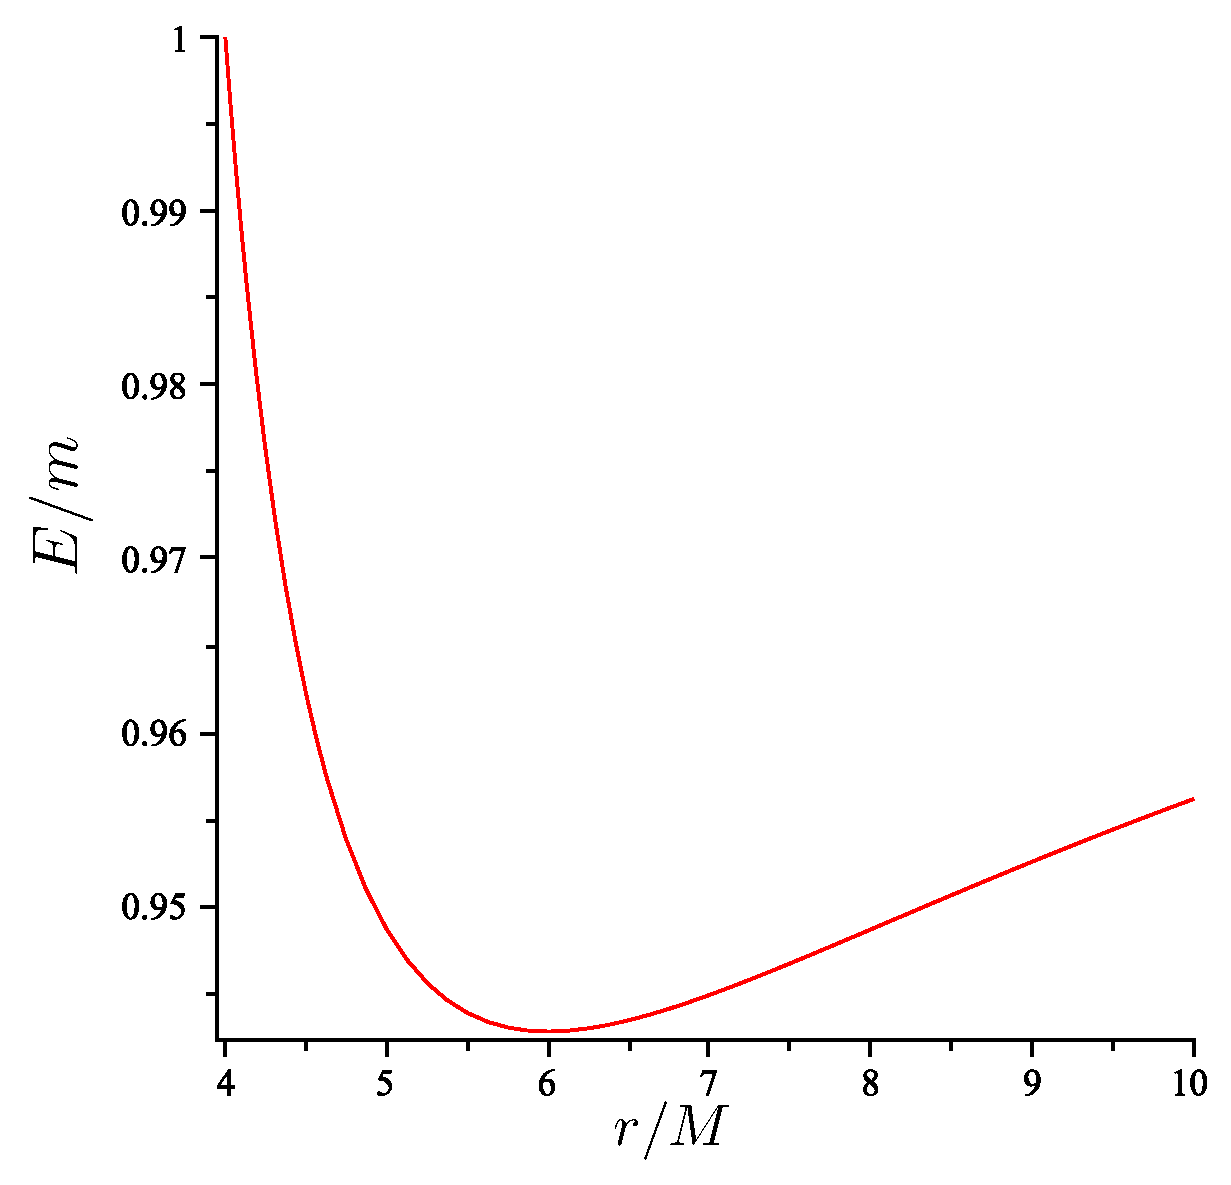
\includegraphics[width=4in]{figures/Eofrplot.pdf}
\caption{A plot of the energy-per-unit mass of a test particle orbiting a Schwarschild black hole as a function of its radial coordinate per the black hole's mass. The plot was created in Maple using equation \ref{eqn:Eschwarz}.}
\end{figure}

\subsection{The Post-Newtonian Expansion}




\Chapter{Introduction to LIGO}
\label{ch:ligo}
%%%% Introduction to LIGO

% The previous chapter elucidated how matter and momenta can affect the spacetime
% to curve around it, and how waves of this curvature propagate outwards from 
% the matter source itself. 
Several methods of detection of gravitational waves have been 
proposed~\cite{PhysRevLett.20.1307,PhysRevD.54.1264,1978SvA....22...36S,
1979ApJ...234.1100D}. Here, we will focus on the interferometric approach
used by the LIGO, Virgo, GEO and the proposed KAGRA
and LIGO-India detectors. We provide a brief description of the interferometric
detectors here, and refer the reader to the text by 
Saulson~\cite{Saulson:1995zi} for a comprehensive treatment.

\section{Design of LIGO}\label{sec:ligo_construction}
\begin{figure}
 \begin{center}
  \scalebox{1}{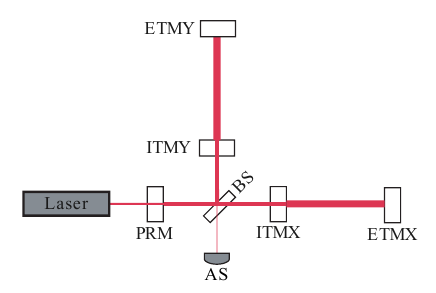
\includegraphics[width=0.6\columnwidth]{figures/ligo/ligo-schematic.png}} 
 \end{center}
\caption{\label{fig:ligo}Schematic of interferometric detectors, like LIGO.}
\end{figure}
%
Interferometric detectors like LIGO comprise of two laser cavities oriented 
orthogonal to each other. The mirrors at either end of each cavity are free to move 
in the horizontal direction, i.e. locally parallel to the surface of the Earth. 
In this restricted direction, for small fluctuations, these mirrors can be
considered as {\it freely-falling} to a good approximation.
The length of the arm cavities largely determines the amount of power stored
in the cavity. 
%
When plus (or cross) polarized gravitational waves pass through, they expand 
one cavity and contract the other, simultaneously, during half of their period,
and vice-versa during the other half. As a result, the difference of the cavities'
lengths (or the differential length) fluctuates, causing a differential fluctuation
in the laser power stored in each cavity. 
% 
Therefore, the effect of incoming gravitational radiation is converted to 
fluctuations of the laser power stored in two spatially orthogonal laser cavities.

Let us consider the schematic in Fig.~\ref{fig:ligo}. The laser source is 
depicted as a rectangle on the most left. The light from it travels through 
the {\it power recycling mirror} (PRM) and reaches the {\it beam 
splitter} (BS). The power recycling mirror reflects back the light 
that leaks out of the cavities in the arms, and in this sense {\it recycles}
the lost laser power. 
The beam splitter splits the main beam into two beams, one that travels along 
the $x$ arm and the other along the $y$ arm. Along the $x$ arm, the {\it end 
test-mass mirror} (ETM-X) and the {\it input test-mass mirror} (ITM-X) form a 
resonant {\it Fabry-Perot} cavity. Similarly for the $y$ arm.
The beams that finally come out of the the two cavities interfere at the beam
splitter and the interference pattern is recorded at the {\it dark port} (DP)
photodiode. This is called so because the two cavities are aligned in a way 
which ensures that the beam coming out of the $x$ arm interferes destructively
with that coming out of the $y$ arm, and hence in the absence of 
gravitational waves the port recording the interference pattern will be 
dark~\footnote{Initial LIGO was aligned at the dark fringe. However, in Advanced
LIGO a DC readout scheme will be used at the output port, 
in order to reduce the readout noise. 
This scheme is sensitive to the light power at the DP.
If the alignment was exactly on a dark fringe then any change in 
the arm lengths would only increase the light at the dark port, and we
would be unable to determine the direction in which the test-mass mirrors were
moving from DC readout. Therefore, the alignment in Advanced LIGO will be
slightly off the dark fringe}.
% 
Finally, a new addition to the Advanced LIGO optics topology is the {\it signal
recycling} (SR) mirror. It sends the signal coming out the dark port back into 
the arm cavities.
The optical system composed of the SR cavity and the arm
cavities forms a
composite resonant cavity, whose resonances and quality
factors can be controlled by the position and
reflectivity of the SR mirror. 
Near its resonances, the detector can gain sensitivity. 
% 
In what follows we discuss the effect of gravitational radiation on 
interferometric detectors, and some of the design choices involved.


Let us consider a $+$-polarized gravitational wave propagating in the 
$z-$direction, with the two arms of the detector along the $x$ and $y$ directions.
We can write down the spacetime metric in the TT gauge at the
location of the detector as
%
\begin{equation}
 \D s^2 = -\D t^2 + (1+h_+)\D x^2 + (1-h_+)\D y^2 + \D z^2.
\end{equation}
% 
% following the discussion in Sec.~\ref{sec:gravitational_radiation}. 
The LIGO 
cavity length is such that it ensures that the time taken by light to travel 
back and forth in it is much smaller comared to the time scale of variations in
$h_+$. Therefore, the time taken by light to make a round-trip between the end
test masses in the $x$ cavity 
% 
\begin{equation}
 t_x \simeq 2L_x (1 + \frac{1}{2}h_+),
\end{equation}
% 
where $L_x$ is the equilibrium length of the $x$ cavity in absence of 
gravitational waves. Here, we have expanded $\sqrt{1+h_+}$ as a Taylor series
and approximated it by keeping terms up to linear order. 
It follows that the light travel time for a round trip in 
the $y$ cavity is
% 
\begin{equation}
 t_y \simeq 2L_y (1 - \frac{1}{2}h_+).
\end{equation}
% 
As the two cavities share the laser source, the same light wavefront will 
return at the beam splitter at different delays in the $x$ than the $y$ cavity. 
Therefore, the change in the phase of the returning light would manifest as a 
phase difference $\delta\phi$ given by
% 
\begin{align}
 \delta\phi &= \Omega_L (t_x - t_y), \\ \nonumber
 &= 2 L\, \Omega_L\,\, h_+ = \dfrac{4\pi L}{\lambda_L}\,h_+,
\end{align}
where $\Omega_L$ ($\lambda_L$) is the frequency (wavelength) of the laser 
light, and we have assumed that $L_x = L_y$ and replaced them with $L$. 


The measurable change in phase $\delta\phi$ is directly 
proportional to the length of the cavities, or the {\it arms} of the detector.
As we aim to observe gravitational wave signals from 
astrophysical sources, which are far enough that the incident signal is
expected to be very weak, this motivates that the two arms be made as 
long as possible before practical considerations become prohibitive.
% 
% In each arm, the end and input test-mass mirrors, $ETM\{X,Y\}$ and 
% $ITM\{X,Y\}$, form a resonant {\it Fabry-Perot} cavity. The end mirrors are 
% highly polished and stabilized in order to maximize their reflectivity. 
% The laser light forms a standing wave in these cavities, and accumulates power.
In addition, the reflectivity of the end mirrors (in each arm) is carefully
controlled, so that each 
wavefront bounces back and forth several times before exiting the cavity and 
interfering at the beam splitter. The net benefit is similar to increasing the
effective length of each arm $L$ by a factor of $\sim 200$ (for LIGO). 
% 
In addition to the layout in Fig.~\ref{fig:ligo}, there are a number of
optical, electronic, mechanical, and electromagnetic sub-systems of LIGO 
detectors that are designed to maximize the sensitivity and efficiency of the detectors.
A treatment of their details is out of the scope of this dissertation, and we
refer the reader to~\cite{lrr-2011-5,Harry:2010zz} for a more technical overview.
% is an {\it output mode
% cleaner} in the path of the output beam between the BS and the DP. The cross 
% section of this beam can be decomposed as Hermite-Gaussian modes, and only the 
% lowest order mode contributes to the readout at the DP. All higher modes
% instead only add to the noise at the readout port, and the output mode 
% cleaner 



\section{Dominant Noise Sources}\label{sec:ligo_noise}

We define the strain signal, $s$, to be the relative change in the length 
of the two arms of the interferometer
% 
\begin{equation}
 s(t) = \dfrac{\Delta L_x - \Delta L_y}{L}.
\end{equation}
% 
The signal $s(t)$ can be written as the sum of two components, (i) the actual
differential arm length change induced by the incident gravitational wave 
$h(t)$ (if present), and (ii) the sum of various noises, $n(t)$, that affect 
the measurement of the difference in the arm lengths $\Delta L$. 
%
As the goal of LIGO is to measure remarkably small length changes, several
sources of noise that propagate to the measurement of $s(t)$ become 
consequential. A few intrinsic to the instrument include the brownian motion
noise in mechanical systems, lossy optics, cross-talk in electromagnetic
systems, noise in control electronics, etc. Additionally, there are noise 
sources in the environment of the detectors, such as wind and ground motion,
fluctuations in the Newtonian gravity due to changes in atmosphere or ground
density, electric coupling from nearby power lines etc. 
%
It is therefore a challenging task to categorize these sources and reduce the
noise to the best extent possible.


Gravitational wave searches in LIGO data are affected by the {\it power
spectral density} of all the noise sources combined. The fundamental noise 
sources that limit the sensitivity of the interferometer in different frequency
ranges are:
% 
\begin{enumerate}
 \item Seismic noise:
 The motion of the ground, whether it be due to earthquakes or due to human 
 activity, couples mechanically to suspended test-mass mirrors at both the ends
 of each arm. This coupling leads to fluctuation in their vertical and horizontal
 position, directly affective the measurement of differential arm length.
 The suspension of mirrors as pendula acts as a low pass filter for seismic
 motion. There are active systems in place as well that sense ground motion and 
 feed the information back to cancel its effect. Seismic noise affects the 
 sensitivity of the detectors at frequecies  $< 40$~Hz.
 \item (Suspension) thermal noise:
 Any physical degree of freedom has an expected energy that depends on the temperature,
 leading to thermal noise in the observations related to that degree of freedom.
 The leading source of thermal noise is the molecular Brownian motion in the
 mirror suspension wires, and in the surface of the mirror. Thermal noise is 
 a low frequency noise that falls off inversely with (the square of) frequency. 
 It dominates  the detector sensitivity in the range $\sim 40-150$~Hz.
 \item Photon shot noise:
 During operation, the interferometer is locked 
 with the optical fields from the two arms interfering destructively at the
 beam splitter, or in other words at a {\it dark fringe}. The number of photons
 that arrive at the readout will be directly proportional to any incident
 gravitational wave signal. The arrival times of the photons at the DP 
 follow Poissonian statistics. Therefore the counting of the number of
 photons that arrive in a given interval of time, $\mathcal{N}$, will have an 
 inherent uncertainty proportional to $\sqrt{\mathcal{N}}$. However, the {\it signal}
 contained in the laser light increases with $\mathcal{N}$, and therefore the 
 signal-to-noise ratio is $\propto \sqrt{\mathcal{N}}$.
 %
 In frequency domain, the shot noise has a flat (or {\it white}) spectrum. 
 However, the arms of the interferometer act as a filter and amplify the effect
 of the shot noise on our ability to measure the incident gravitational wave
 with increasing frequency. As a result, this noise source dominates over all
 others at $f\gtrsim 1$~kHz.
\end{enumerate}
% 
We refer the reader to~\cite{Saulson:1995zi} for a detailed treatment of these
noise sources, which is out of scope of this dissertation. 

Apart from these continuous noise sources, there is another class of noise 
that plagues our ability to systematically extract signals embedded in detector
data called {\it glitches}. Glitches are transient by definition, and have a 
variety of frequency spectrum and sources. More importantly, if not correctly 
identified with their cause, they could be unpredictable. For instance, the 
falling of a 
heavy object could shake optics and lead to a sharp rise in the noise level
in the differential arm length output. There are mechanisms being developed to 
identify and classify glitches in Advanced LIGO and Virgo, within the Detector
characterization group. There are also algorithms in place that allow search 
methods to differentiate between signals and glitches based on their frequency
spectrum and evolution.


% % This section is completely un-necessary
% \section{Calibration of LIGO}\label{sec:ligo_calibration}
% \begin{figure}
%  \begin{center}
%   \scalebox{1}{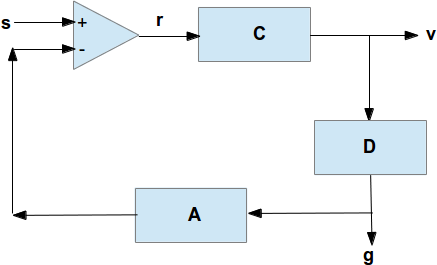
\includegraphics[width=0.6\columnwidth]{figures/ligo/ligo-control-loop.png}} 
%  \end{center}
% \caption{\label{fig:ligo_calibration}Model for the control loop of the LIGO
% length sensing and control system.}
% \end{figure}
% 
% The signal recorded at the output port $v(t)$ is proportional to the effect of 
% the differential motion of the mirrors in the two arms of the interferometer.
% This signal is itself used in a control loop to further stabilize the free-falling
% masses by actuating on them. Therefore the effect of the gravitational waves alone, 
% $s(t)$, has to be decoded from $v(t)$ by understanding this control loop.
% 
% Let us model this length sensing control loop as in
% Fig.~\ref{fig:ligo_calibration}. All the blocks symbolize the transfer function
% of a particular logical block, which is the ratio of its output to its input.
% All quantities hereafter will be in frequency domain, while the transfer 
% functions themselves could be slowly varying in time as well. 
% Block $C$ denotes the 
% length sensing function. It measures the response of the arm cavities to 
% gravitational waves. Block $D$ converts the output of block $C$, i.e. the 
% fluctuation in the differential arm length into a control signal that is sent
% to block $A$. Block $A$ is the {\it actuation} function that reacts to the 
% control signal and actuates upon the suspended masses in a way so as to 
% stabilize them. 
% 
% We calculate the transfer function $G$ between the readout and the actual 
% gravitational wave signal as
% %
% \begin{equation}
%  \begin{split}
%   v = C\, r ;\hspace{5mm} g &= D\, v = CD\, r ;\hspace{5mm} r = s - A\, g = s - CDA\, r, \\
%   &\Rightarrow G \defeq \dfrac{s}{v} = \dfrac{1 + CDA}{C}.
%  \end{split}
% \end{equation}
% % 
% The process of calibrating interferometer data therefore involves measuring 
% the aforementioned transfer functions to high accuracy and using them to obtain 
% the final data channel containing the possible gravitational wave signal.



\section{Detector response to Gravitational wave polarizations}\label{sec:ligo_response}
\begin{figure}
 \begin{center}
  \scalebox{1}{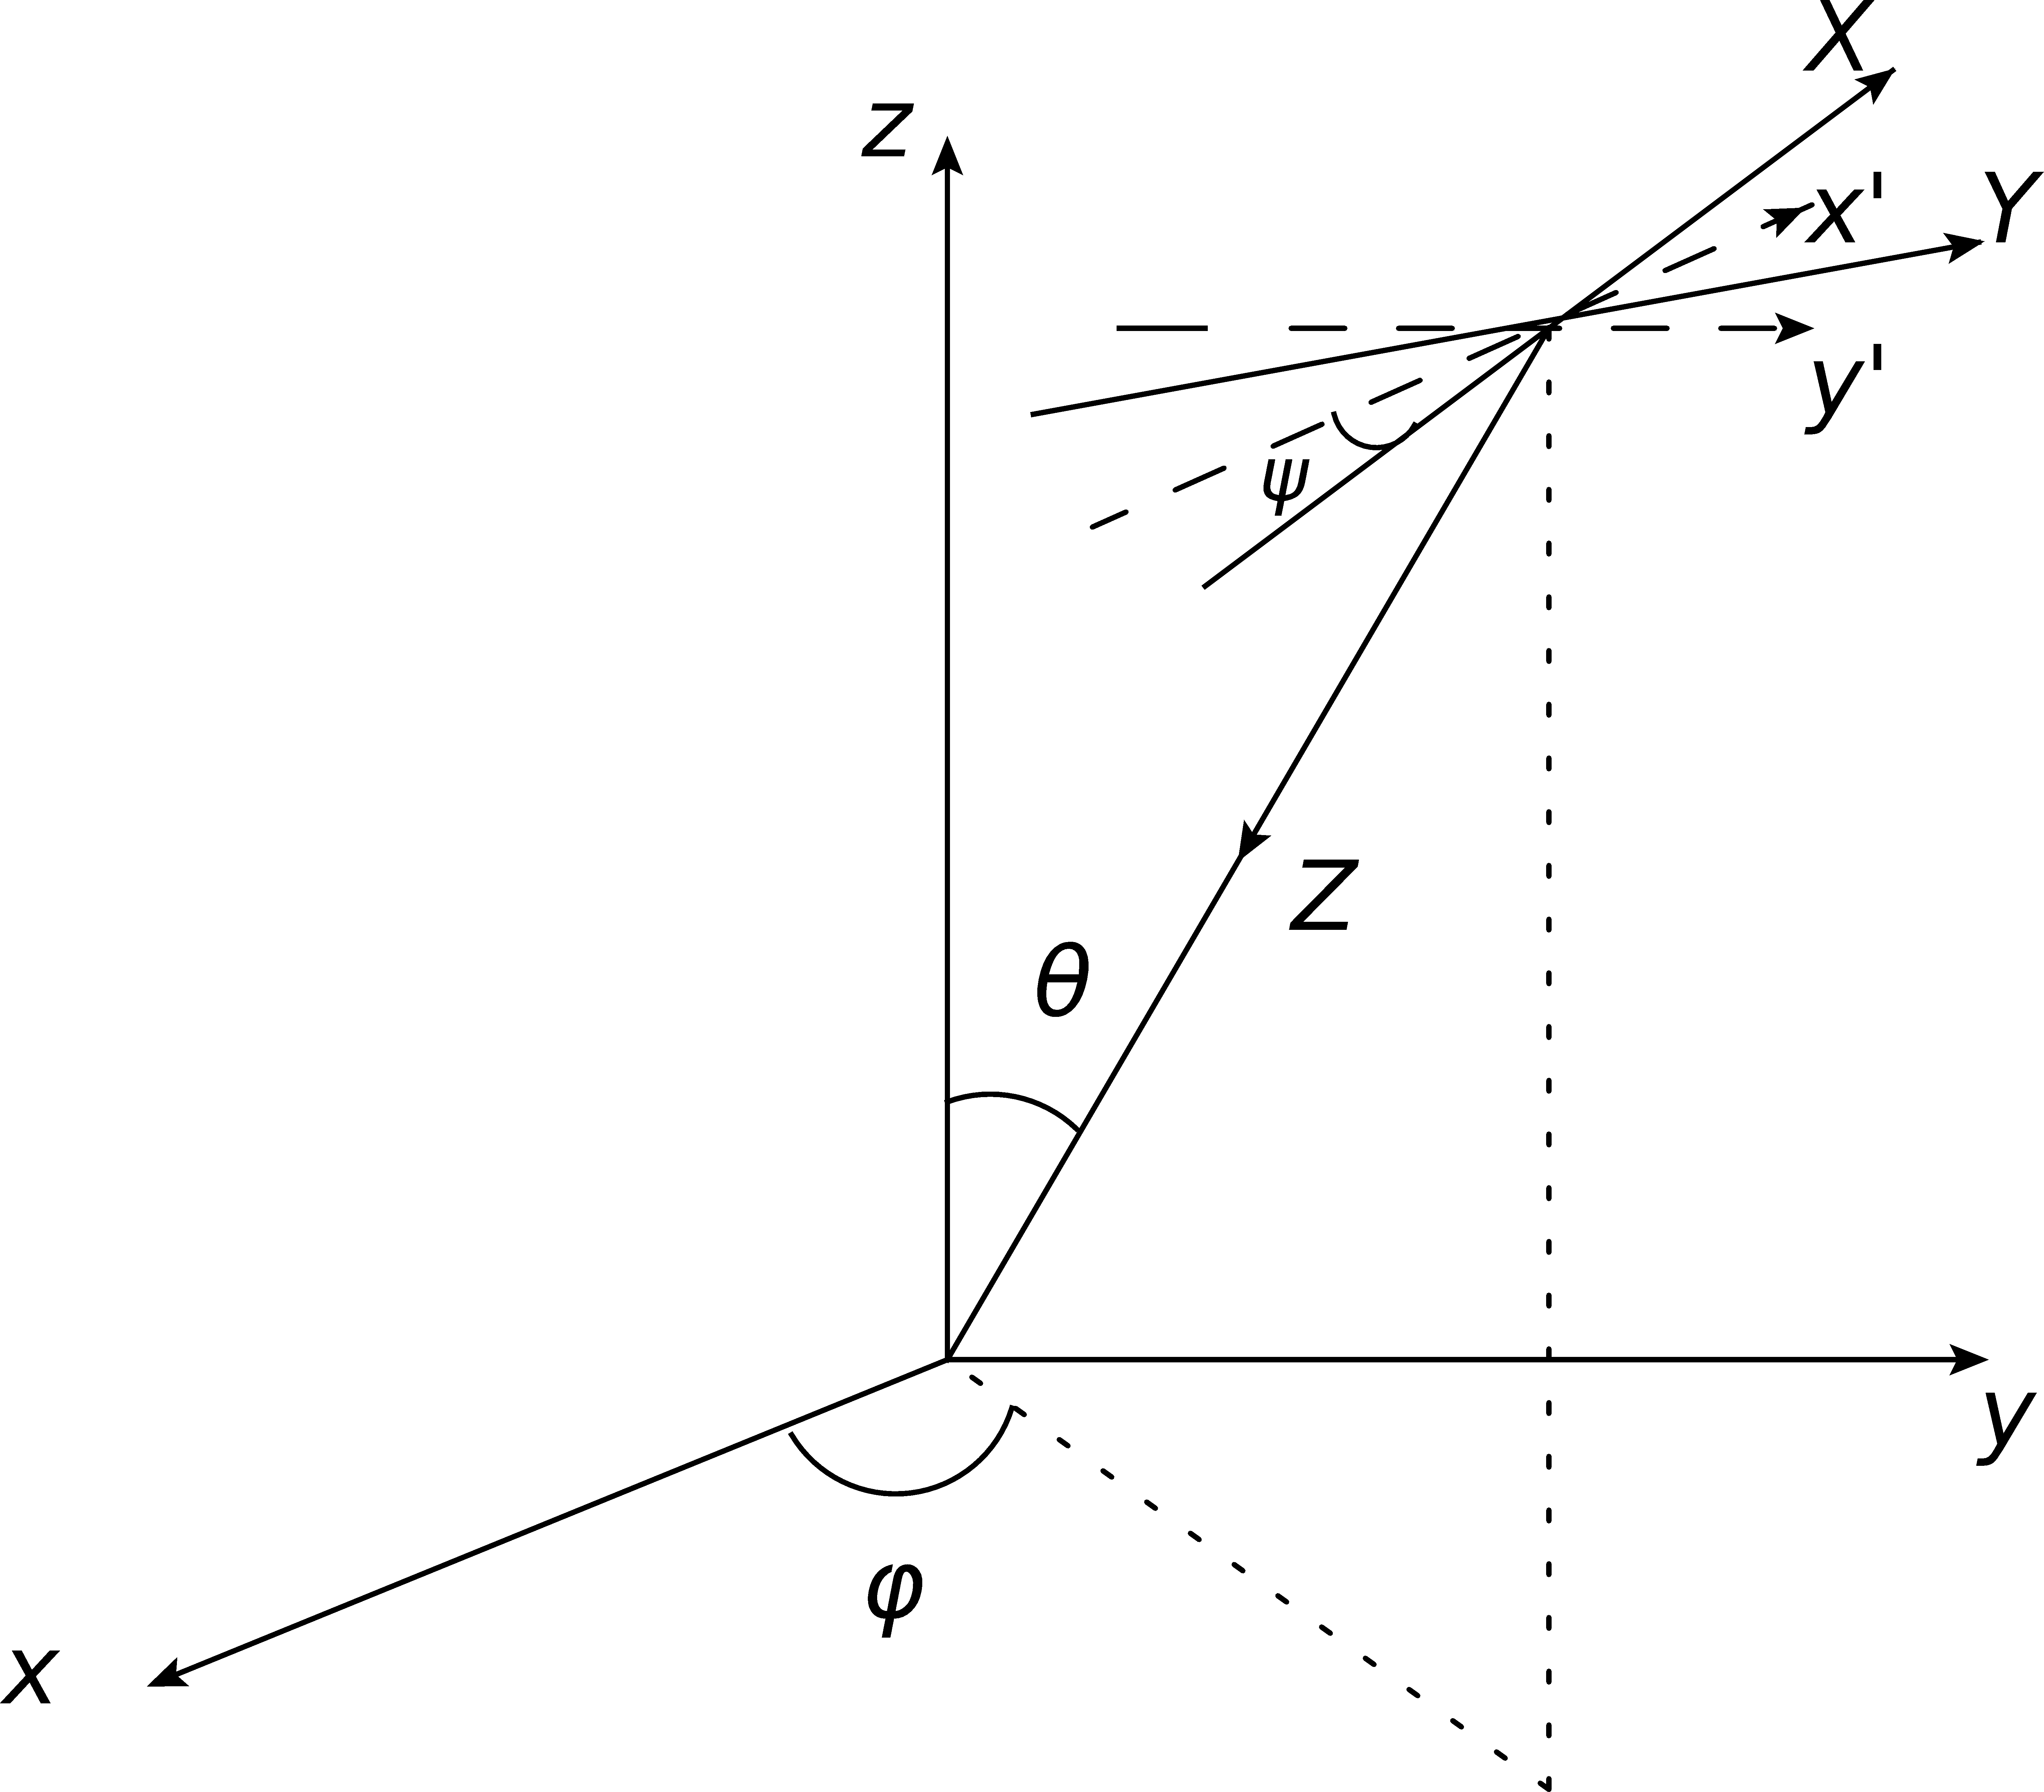
\includegraphics[width=0.6\columnwidth]{figures/ligo/radiation-detector-frame.png}} 
 \end{center}
\caption{\label{fig:radiation_detector_frames}
The angles $\{\theta,\phi\}$ show the relative orientation of the radiation 
$(X,Y,Z)$ and the detector $(x,y,z)$ frames. $x'$ and $y'$ axes are parallel 
to the $x$ and $y$ axes, respectively. $\psi$ is the angle by which the radiatoin
frame is rotated, around the line of sight.}
\end{figure}

We start with defining the radiation frame which has its $x-y$ plane in the 
plane of the sky if one is looking towards the source. The line connecting the 
source and the detector defines its $z-$axis. Therefore we can determine the 
polar angles $(\theta,\phi)$ that point along the $z-$axis of the 
radiation frame. Finally, $\psi$ is the angle between the $x-$axis of the 
radiation frame and the plane made by joining the $x-$arm of the detector and
the $z-$axis of the radiation frame. The detector frame is intuitively defined
by defining the $x$ and $y$ axes along the two arms with the $z-$axis coming
out of the plane of the detector on Earth.

It can be shown that the polarization amplitudes in the radiation frame depend 
on the {\it inclination} angle $\iota$ between the orbital (or total) angular 
momentum of the binary and the line of sight from the detector to the source
as~\cite{SathyaSchutzLRR}
% 
\begin{equation}\label{eq:h_inclination}
 h_+ = \frac{1}{2}(1 + \cos^2\iota)\,h_0\cos\Phi(t); \hspace{10mm} h_\times = \cos\iota\,h_0\sin\Phi(t).
\end{equation}
%
$h_0$ is an overall amplitude that varies slowly in time compared to the 
instantaneous gravitational wave phase $\Phi(t)$. 
In the radiation frame the tensorial metric perturbation can be written as 
(bold fonts indicate tensors or vectors with indices suppressed)
\begin{equation}
 {\bf h} = h_+{\bf e_+} + h_\times{\bf e_\times}
\end{equation}
% 
where the basis tensors are defined as
% 
\begin{equation}
 {\bf e_+}\defeq {\bf e^R_x}\otimes {\bf e^R_x} - {\bf e^R_y}\otimes {\bf e^R_y}; \hspace{10mm}
 {\bf e_\times}\defeq {\bf e^R_x}\otimes {\bf e^R_y} + {\bf e^R_y}\otimes {\bf e^R_x},
\end{equation}
% 
with ${\bf e^R_x}$ and ${\bf e^R_y}$ being unit vectors along the $x$ and $y$ 
axes of the radiation frame. Next we define the {\it detector tensor}, which 
can be thought of as the projection tensor for the detector, as
% 
\begin{equation}
 {\bf d} \defeq L({\bf e^D_x}\otimes {\bf e^D_x} - {\bf e^D_y}\otimes {\bf e^D_y}),
\end{equation}
% 
where ${\bf e^D_x}$ and ${\bf e^D_y}$ are unit vectors along the $x$ and $y$ 
axes of the detector frame, and they point along the direction of the arms from 
the central beam splitter. $L$ is the length of each arm of the interferometer. 
The change in length of the arms $\delta L(t)$ can therefore be obtained as the
scalar product between the ${\bf h}$ tensor and the detector tensor, i.e.
% 
\begin{equation}
 \delta L(t) = {\bf d}\cdot {\bf h} \defeq d_{ij}h^{ij}
\end{equation}
% 
This allows the strain produced in the arms to be written as
% 
\begin{equation}\label{eq:h_strain_antenna}
 h(t)\defeq\frac{\delta L}{L} = F_+(\theta, \phi, \psi) h_+ + F_\times(\theta, \phi, \psi) h_\times,
\end{equation}
where the functions $F_+$ and $F_\times$ can be found using the geometry in
Fig.~\ref{fig:radiation_detector_frames} as the scalar product of the basis tensors
${\bf e_+}$ and  ${\bf e_\times}$ with the detector tensor~\cite{SathyaSchutzLRR},
% 
\begin{equation}\label{eq:fpluscross}
 \begin{split}
  F_+ &= \frac{1}{2}(1 + \cos^2\theta)\cos(2\phi)\cos(2\psi) - \cos(\theta)\sin(2\phi)\sin(2\psi), \\
  F_\times &= \frac{1}{2}(1 + \cos^2(\theta))\cos(2\phi)\sin(2\psi) + \cos(\theta)\sin(2\phi)\cos(2\psi).
 \end{split}
\end{equation}
These two functions are called the {\it antenna patterns} of the detector, 
and they define the response of the detector to incoming gravitational 
radiation governed purely due to the relative geometry between the source and 
the detector itself. Finally, collecting Eq.~\eqref{eq:h_inclination} and
Eq.~\eqref{eq:h_strain_antenna} we can write the strain $h(t)$ seen by the 
detector as
% 
\begin{equation}
 h(t) = F_+ h_+ + F_\times h_\times = \mathcal{A} h_0 \cos(\Phi(t) - \Phi_0),
\end{equation}
% 
where $\Phi(t)$ has the same meaning as in Eq.~\eqref{eq:h_inclination}, and
% 
\begin{equation}
\begin{split}
 \mathcal{A} &\defeq \left(\left(\frac{1}{2}F_+(1+\cos^2\iota)\right)^2 + \left(F_\times\cos\iota\right)^2\right)^{1/2}, \\
 \Phi_0 &\defeq \tan^{-1}\left( \frac{2F_\times\cos\iota}{F_+(1+\cos^2\iota)}\right),
\end{split}
\end{equation}
% 
are combinations of the antenna patterns and the inclination angle folded 
into a constant amplitude and phase change. 



\Chapter{Search template banks for low-mass binary black holes in the 
Advanced gravitational-wave detector era}
\label{ch:EOBF2_Effectualness}
%%%%%%%%%%%%%%%%%%%%%%%%%%%%%%%%%%%%%%%%%%%%%%%%%%%%%%%%%%%%%%%%%%%%%%%%%%%%%%%
%%% Study of the effectualness of 2PN non-spinning metric with PN/EOB templates
%%%%%%%%%%%%%%%%%%%%%%%%%%%%%%%%%%%%%%%%%%%%%%%%%%%%%%%%%%%%%%%%%%%%%%%%%%%%%%%

\section{Introduction}
Over the last decade, there has been tremendous progress towards the
first direct detection of gravitational waves. Construction of the Advanced
Laser Interferometer Gravitational-Wave Observatory (aLIGO) is underway, with
completion scheduled for 2014~\cite{Harry:2010zz}. Similar upgrades to
the French-Italian Virgo detector~\cite{aVIRGO} have commenced and construction
of the Japanese KAGRA detector has begun~\cite{Somiya:2011np}.  When these
second-generation gravitational-wave detectors reach design sensitivity, they
will increase the observable volume of the universe by a thousandfold or
more~\cite{aLIGOsensitivity}, compared to the first-generation detectors.

The inspiral and merger of binary black holes (BBHs) are expected to be an important source for detection by
aLIGO~\cite{300yrsofGravitation}.  The rate of BBH coalescences that will be
observed by aLIGO at design sensitivity is estimated to be between
$0.2\,\mathrm{yr}^{-1}$ and $1000\,\mathrm{yr}^{-1}$~\cite{LSCCBCRates2010}.
Accurate knowledge of the gravitational-wave signals generated by BBHs is
crucial for detecting and extracting information about these sources.  
To provide such waveforms, the effective one body (EOB)
model~\cite{EOBOriginalBuonannoDamour} has been calibrated to numerical
simulations of black hole
mergers~\cite{EOBNR01,EOBNRdevel01,EOBNRdevel02,EOBNRdevel03,EOBNRdevel04,EOBdevel01,EOBdevel02,BuonannoEOBv2Main}.
A new EOB waveform family (called EOBNRv2) has been recently proposed that
incorporates information from several non-spinning BBH simulations, with black
hole ring-down quasi-normal modes~\cite{BHRDQNMs,BHPTMinoSasaki} attached to
provide a complete BBH waveform~\cite{BuonannoEOBv2Main}.  The EOBNRv2
waveform is believed to be sufficiently accurate to search for non-spinning
BBH signals in the aLIGO sensitive band (10-1000 Hz). 

Past searches for
BBHs~\cite{Colaboration:2011nz,Abadie:2010yb,Abbott:2009qj,Abbott:2009tt,Messaritaki:2005wv}
used matched-filtering~\cite{Wainstein:1962,Allen:2005fk} to search for
coalescing compact binaries. These searches divided the BBH mass space into a
\emph{low-mass} region with $M = m_1 + m_2 \lesssim 25\, M_\odot$ and a
\emph{high-mass} region with $M \gtrsim 25 \, M_\odot$. In this chapter, we
focus attention on BBH systems with component masses between $3 \, M_{\odot}
\lesssim m_1, m_2 \lesssim 25 M_{\odot}$, which encompasses mass distribution
of black hole candidates observed in low-mass X-ray
binaries~\cite{Ozel:2010su}. aLIGO will be able to detect coalescing BBH
systems with component masses $m_1 = m_2 = 25 \, M_{\odot}$ to a maximum
distance of up to $\sim 3.6$~Gpc.  Since we do not know \emph{a priori} the
masses of BBHs that gravitational-wave detectors will observe, searches use a
\textit{bank} of template waveforms which covers the range of BBH component
masses of interest~\cite{Sathyaprakash:1991mt,Balasubramanian:1995bm}.  This
technique is sensitive to the accuracy of the waveform templates that are used
as filters and the algorithm used to place the template
waveforms~\cite{FittingFactorApostolatos}. An accurate template bank is
required as input for matched filter
searches in the Fouier domain~\cite{Allen:2005fk}, as well as newer search algorithms such as the
singular value
decomposition~\cite{Cannon:2010qh}. 

In this chapter, we investigate three items of importance to advanced-detector
BBH searches: First, we study the accuracy of template placement algorithms
for BBH searches using EOBNRv2 waveforms. Optimal template placement requires
a metric for creating a grid of waveforms in the desired region of parameter
space~\cite{OwenTemplateSpacing}, however no analytic metric exists for the
EOBNRv2 waveform. In the absence of such a metric, we construct a template
bank using the second-order post-Newtonian hexagonal placement
algorithm~\cite{SathyaBankPlacementTauN,BabaketalBankPlacement,SathyaMetric2PN,Cokelaer:2007kx}.
This metric is used to place template grid points for the aLIGO zero-detuning
high power sensitivity curve~\cite{aLIGONoiseCurve} and we use EOBNRv2
waveforms at these points as search templates.  We find that the existing
algorithm works well for BBHs with component masses in the range $3 M_\odot
\le m_1, m_2 \le 25\, M_\odot$.  For a template bank constructed with a
minimal match of $97\%$ less than $1.5\%$ of non-spinning BBH signals have a
mismatch greater than $3\%$. We therefore conclude that the existing bank
placement algorithm is sufficiently accurate for non-spinning BBH searches in
this mass region.  Second, we investigate the mass range in which the
(computationally less expensive) third-and-a-half-order TaylorF2
post-Newtonian
waveforms~\cite{Sathyaprakash:1991mt,Cutler:1994ys,Droz:1999qx,PNFluxEnergy3PN01,PNFluxEnergy3PN02,Jaranowski:1999qd,Jaranowski:1999ye,Damour:2001bu,KidderPN,Blanchet3PN}
can be used without significant loss in event rate, and where full
inspiral-merger-ringdown EOBNRv2 waveforms are required. We construct a
TaylorF2 template bank designed to lose no more than $3\%$ of the matched
filter signal-to-noise ratio and use the EOBNRv2 model as signal waveforms.
We find that for non-spinning BBHs with $M \lesssim 11.4\,M_{\odot}$, the
TaylorF2 search performs as expected, with a loss of no more than $10\%$ in
the event rate. For higher masses larger event rate losses are observed. A
similar study was performed in Ref.~\cite{CompTemplates2009} using an older
version of the EOB model and our results are quantitatively similar. We
therefore recommend that this limit is used as the boundary between TaylorF2
and EOBNRv2 waveforms in Advanced LIGO searches.  Finally, we investigate the
effect of modes other than the dominant $l = m = 2$ mode on BBH searches in
aLIGO.  The horizion distance of aLIGO (and hence the event rate) is computed
considering only the dominant mode of the emitted gravitational waves, since
current searches only filter for this mode~\cite{LSCCBCRates2010}. However,
the inclusion of sub-dominant modes in gravitational-wave template could
increase the reach of aLIGO~\cite{McKechan:2011ps,Pekowsky:2012sr}. If we
assume that BBH signals are accurately modeled by the EOBNRv2 waveform
including the five leading modes, we find that for systems with $(m_1/m_2)\leq
1.68$ or inclination angle: $\iota \geq 2.68$ or $\iota \leq 0.31$ radians, 
there is no significant loss in the total possible signal-to-noise ratio
due to neglecting modes other than $l = m = 2$ in the template waveforms,
if one uses a $97\%$ minimal-match bank placed using the hexagonal bank placement
algorithm ~\cite{SathyaBankPlacementTauN,BabaketalBankPlacement,SathyaMetric2PN,Cokelaer:2007kx}.
However, for systems with mass-ratio ($q$) $\geq 4$ and $1.08\leq\iota\leq 2.02$, including higher order modes could increase
the signal-to-noise ratio by as much as $8\%$ in aLIGO. This increase in
amplitude may be offset by the increase in false alarm rate from implementing
searches which also include sub-dominant waveform modes in templates, so we encourage the 
investigation of such algorithms in real detector data.

The remainder of this chapter is organized as follows: In Sec.~\ref{s:waveforms}
we review the gravitational waveform models used in this study. In
Sec.~\ref{s:results} we present the results of large-scale Monte Carlo signal
injections to test the effectualness of the template banks under
investigation. Finally in Sec.~\ref{s:conclusions} we review our findings and
reccomendations for future work.

\section{Waveforms and Template Bank Placement}
\label{s:waveforms}
\subsection{Waveform Approximants}
The dynamics of a BBH system can be broadly divided into three regimes: (i) The 
early inspiral, when the separation between the black holes is large and their
velocity is small, can be modeled
using results from post-Newtonian (PN)
theory~\cite{PNtheoryLivingReviewBlanchet}. The gravitational-wave phasing of
non-spinning binaries is available up to 3.5PN
order~\cite{PNFluxEnergy3PN01,PNFluxEnergy3PN02,Jaranowski:1999qd,Jaranowski:1999ye,Damour:2001bu,KidderPN,Blanchet3PN}.
(ii) Accurately modeling the late-inspiral and merger requires the numerical
solution of the Einstein
equations~\cite{Pretorius2005,Pretorius2006,BBHNRScheel,BBHNRGonzalezq10,BBHNRPollney,BBHNRLoustoq10,Buchman:2012dw}.
(iii) The final ring-down phase can be modeled using a super-position of
quasi-normal modes (QNMs) which describe the oscillations of the perturbed Kerr
black-hole that is formed from the
coalescence~\cite{BHRDQNMs,BHPTMinoSasaki}. 

Numerical simulation of BBH systems are computationally expensive, and results
are only available for a relatively small number of binary systems (see
e.g.~\cite{Ajith:2012tt}).  The EOB model~\cite{EOBOriginalBuonannoDamour}
provides a framework for computing the gravitational waveforms emitted during
the inspiral and merger of BBH systems.  By attaching a QNM waveform and
calibrating the model to numerical relativity (NR) simulations, the EOB
framework provides for accurate modeling of complete BBH waveforms (EOBNR). The
EOBNR waveforms can be computed at relatively low cost for arbitrary points in the
waveform parameter
space~\cite{EOBNR01,EOBNRdevel01,EOBNRdevel02,EOBNRdevel03,EOBNRdevel04,EOBdevel01,EOBdevel02,BuonannoEOBv2Main}.
In particular the EOB model has recently been tuned against high-accuracy
numerical relativity simulations of non-spinning BBHs of mass-ratios
$q=\{1,2,3,4,6\}$, where $q\,\equiv \, m_1/m_2$~\cite{BuonannoEOBv2Main}; we
refer to this as the EOBNRv2 model, which we review the major features of
below. Throughout, we set $G=c=1$.

The EOB approach maps the fully general-relativistic dynamics of the two-body
system to that of an \textit{effective} mass moving in a deformed
Schwarzschild spacetime~\cite{EOBOriginalBuonannoDamour}. The physical
dynamics is contained in the deformed-spacetime's metric coefficients, the EOB
Hamiltonian~\cite{EOBOriginalBuonannoDamour}, and the radiation-reaction
force. In polar coordinates $(r,\Phi)$, the EOB metric is written as
\begin{equation}\label{eq:dsEOB}
\D s_{\eff}^2 = -A(r)\D t^2 + \dfrac{A(r)}{D(r)}\D r^2 + r^2\left(\D\Theta^2 + \sin^2\Theta \D\Phi^2\right).
\end{equation}
The geodesic dynamics of the \textit{effective} mass $\mu\,=\,m_1 m_2 /
M$ in the background of Eq.~\eqref{eq:dsEOB} is described by an effective
Hamiltonian $H^{\eff}$~\cite{EOBOriginalBuonannoDamour,PadeAD}.
The EOBNRv2 model uses Pade-resummations of the third-order post-Newtonian
Taylor expansions of the metric coefficients $A(r)$ and $D(r)$, with
additional 4PN and 5PN coefficients that are
calibrated~\cite{EOBNRdevel01,EOBNRdevel02,EOBNRdevel03,EOBNRdevel04,BuonannoEOBv2Main} 
to ensure that the dynamics agrees closely with NR simulations of comparable
mass binaries.

Gravitational waves carry energy and angular momentum away from the binary,
and the resulting radiation-reaction force $\hat{F}_{\Phi}$ causes the orbits
to shrink. This is related to the energy flux as 
\begin{equation}
\hat{F}_{\Phi} = -\dfrac{1}{\eta \hat{\Omega}} \dfrac{\D E}{\D t} = -\dfrac{1}{\eta v^3} \dfrac{\D E}{\D t},
\end{equation}
where, $v=(\hat{\Omega})^{1/3}=(\pi Mf)^{1/3}$ and $f$ is the instantaneous
gravitational-wave frequency. The energy flux $\D E/\D t$ is obtained by
summing over the contribution from each term in the multipole expansion of the
waveform, i.e. 
\begin{equation}
\frac{\D E}{\D t} = \frac{\hat{\Omega}^2}{8\pi} \Sum_{l}\Sum_{m} \left|\frac{\mathcal{R}}{M} h_{lm}\right|^2.
\end{equation}
$\mathcal{R}$ is the physical distance to the binary, and $h_{lm}$ are
the multipoles of the waveform when it is decomposed in spin weighted
spherical harmonic basis as
\begin{equation}
h_+ - \ii h_{\times} = \dfrac{M}{\mathcal{R}} \Sum^{\infty}_{l=2} \Sum^{m=l}_{m = -l} Y^{lm}_{-2}\, h_{lm},
\end{equation}
where $Y^{lm}_{-2}$ are the spin weighted spherical harmonics, and $h_+$ and
$h_{\times}$ are the two orthogonal gravitational wave polarizations. These
waveform multipoles depend on the coordinates and their conjugate momenta, and
their Taylor expansions were re-summed as products of individually re-summed
factors~\cite{DamourFluxhlm01}, 
\begin{subequations}\label{eq:hlmdef}
\begin{align}
h_{lm} &= h^F_{lm} N_{lm}\label{eq:hNQC},\\
h^F_{lm} &= h^{(N,\epsilon)}_{lm} \hat{S}_{\eff}^{(\epsilon)} T_{lm} e^{\ii\delta_{lm}} (\rho_{lm})^l\label{eq:hNoNQC};
\end{align}
\end{subequations}
where $\epsilon$ is $0$ if $\left( l+m\right)$ is even, and is $1$ otherwise. This
factorized-re-summation of the waveform multipoles ensures agreement with NR
waveform multipoles~\cite{EOBNRdevel01,EOBNRdevel02,EOBNR01}.  The first
factor $h^{(N,\epsilon)}_{lm}$ is the re-summation of the Newtonian order
contribution and the second factor  $\hat{S}_{\eff}^{(\epsilon)}$ is the
source term, given by the mass or the current moments of the binary in the EOB
formalism~\cite{DamourFluxhlm01,BuonannoEOBTerms}. The tail term $T_{lm}$ is
the re-summation of the leading order logarithmic terms that enter into the
transfer function of the near-zone multipolar waves to the
far-zone~\cite{BuonannoEOBTerms}. The last term $N_{lm}$ attempts to capture
the non-circularity of the quasi-circular orbits.  While calculating the
energy flux in this study we follow exactly the prescription of
Ref.~\cite{BuonannoEOBv2Main}, which calibrates the coefficients of the flux
so that resulting EOB waveform multipoles reproduce their NR counterparts with
high accuracy.

We use the EOBNRv2 Hamiltonian and flux in the equations of motion for the
binary, given by
\begin{subequations}\label{eq:EOBHamiltonianEqs}	
 \begin{align}
\dfrac{\D r}{\D\hat{t}} &\equiv \dfrac{\partial \hat{H}^{\real}}{\partial p_r} = \dfrac{A(r)}{\sqrt{D(r)}}\dfrac{\partial \hat{H}^{\real}}{\partial p_{r*}} (r, p_{r*}, p_{\Phi}) ,\\
\dfrac{\D\Phi}{\D\hat{t}} &\equiv \hat{\Omega} = \dfrac{\partial \hat{H}^{\real}}{\partial p_{\Phi}} (r, p_{r*}, p_{\Phi}) , \\ 
\dfrac{\D p_{r_*}}{\D\hat{t}} &= -\dfrac{A(r)}{\sqrt{D(r)}} \dfrac{\partial \hat{H}^{\real}}{\partial r} (r, p_{r*}, p_{\Phi}) ,\\
\dfrac{\D p_{\Phi}}{\D\hat{t}} &= \hat{F}_{\Phi}(r, p_{r*}, p_{\Phi}) ;
  \end{align}
\end{subequations}
where, $\hat{t}\,(\equiv t/M)$ is time in dimensionless units. 

To obtain the initial values of the coordinates $(r,\Phi,p_{r_*},p_{\Phi})$ that the
system starts out in, we use the conditions for motion on spherical orbits derived in
Ref.\cite{Buonanno:2005xu}, where they treat the case of a generic precessing binary.
We take their non-spinning limit to define the initial configuration of the binary, requiring
\begin{subequations}
\begin{align}\label{eq:IniHr}
\dfrac{\partial\hat{H}^{\real}}{\partial r} &= 0,\\ \label{eq:IniHpr}
\dfrac{\partial\hat{H}^{\real}}{\partial p_{r_*}} &= \dfrac{1}{\eta}\dfrac{\D E}{\D t}\dfrac{(\partial^2\hat{H}^{\real}/\partial r\partial p_{\Phi} )}{(\partial\hat{H}^{\real}/\partial p_{\Phi})(\partial^2\hat{H}^{\real}/\partial r^2)}, \\\label{eq:IniHpphi}
\dfrac{\partial\hat{H}^{\real}}{\partial p_{\Phi}} &= \hat{\Omega}_0,
\end{align}
\end{subequations}
where $\hat{\Omega}_0 = \pi Mf_0$, with $f_0$ being the starting gravitational wave frequency. Simplifying Eq.\eqref{eq:IniHr}, and ignoring the terms involving $p_{r_*}$, as $p_{r_*}\ll p_{\Phi}/r$ in the early inspiral, we get a relation between $p_{\Phi}$ and $r$:
\begin{equation}
p_{\Phi}^2 = \dfrac{r^3A'(r)}{2A(r) - rA'(r)} \\ \label{eq:Inipphi},
\end{equation}
where the prime($'$) denotes $\partial/\partial r$. Substituting this in Eq.\eqref{eq:IniHpphi}, we get the relation:
\begin{equation}
\dfrac{A'(r)}{2r\left(1 + 2\eta\left(\dfrac{A(r)}{\sqrt{A(r)-\frac{1}{2}r\,A'(r)}} - 1\right)\right)} = \hat{\Omega}_0^2.\\ \label{eq:Inir}
\end{equation} 
Thus, between Eq.\eqref{eq:Inir} and Eq.\eqref{eq:Inipphi}, we get the initial values 
of $(r, p_{\Phi})$, corresponding to the initial gravitational wave frequency $f_0$,
and by substituting these into Eq.~\ref{eq:IniHpr}, we obtain the initial value 
of $p_{r_*}$.
With these values, we integrate the equations of motion to obtain the evolution 
of the coordinates and momenta $(r(t),\Phi(t),p_r(t),p_{\Phi}(t))$ over the 
course of inspiral, until the light-ring is reached. In the EOB model, the 
light-ring is defined as the local maximum of the orbital frequency 
$\hat{\Omega}$. From the coordinate evolution, we also calculate $h^F_{lm}(t)$,
which is the analytic expression
for the waveform multipole without the non-quasi-circular correction factor
(defined in Eq.~\eqref{eq:hNoNQC}). While generating $h^F_{lm}(t)$ from the
dynamics, the values for the free parameters in the expressions for
$\delta_{lm}$ and $\rho_{lm}$, are taken from Eqn.[38a-39b] of
Ref.~\cite{BuonannoEOBv2Main}, where they optimize these parameters to
minimize the phase and amplitude discrepancy between the respective EOB
waveform multipoles and those extracted from NR simulations.

The EOB ringdown waveform is modeled as a sum of $N$ quasi-normal-modes
(QNMs)~\cite{EOBNRdevel01,EOBNRdevel02,EOBNRdevel04,BHRDQNMs}
\begin{equation}
h_{lm}^{\RD}(t) = \Sum^{N-1}_{n=0}A_{lmn}e^{-\ii\sigma_{lmn}(t-t_{lm}^{\mathrm{match}})},
\end{equation}
where $N=8$ for the model we consider. The matching time
$t_{lm}^{\mathrm{match}}$ is the time at which the inspiral-plunge and the
ringdown waveforms are attached and is chosen to be the time at which the
amplitude of the inspiral-plunge part of $h_{lm}(t)$ peaks $\left(\mathrm{i.e.}\,
t^{lm}_{\peak}\right)$~\cite{EOBNRdevel01,BuonannoEOBv2Main}. The complex
frequencies of the modes  $\sigma_{lmn}$  depend on the mass $M_f$ and spin
$a_f$ of the BH that is formed from the coalescence of the binary.
We use the relations of Ref.~\cite{BuonannoEOBv2Main}, given by 
\begin{subequations}
\begin{align}
\dfrac{M_f}{M} &= 1 + \left(\sqrt{\frac{8}{9}}-1\right)\eta - 0.4333\eta^2 - 0.4392\eta^3,\\
\dfrac{a_f}{M} &= \sqrt{12}\eta - 3.871\eta^2 + 4.028\eta^3.
\end{align}
\end{subequations}
Using the mass and spin of the final BH, the complex frequencies of the QNMs
can be obtained from Ref.~\cite{BHRDQNMs}, where these were calculated using
perturbation theory. The complex amplitudes $A_{lmn}$ are determined by a
hybrid-comb numerical matching procedure described in detail in Sec.II C of
Ref.~\cite{BuonannoEOBv2Main}.

Finally, we combine the inspiral waveform multipole $h_{lm}(t)$ and the
ringdown waveform $h^{\RD}(t)$ to obtain the complete inspiral-merger-ringdown
EOB waveform $h^{\textrm{IMR}}(t)$, 
\begin{equation}
h^{\textrm{IMR}}_{lm}(t) = h_{lm}(t)\Theta(t^{\mathrm{match}}_{lm}-t) + h^{\RD}(t)\Theta(t-t^{\mathrm{match}}_{lm}),
\end{equation}
where $\Theta(x)=1$ for $x\geq 0$, and 0 otherwise. These multipoles are
combined to give the two orthogonal polarizations of the gravitational
waveform, $h_+$ and $h_{\times}$, 
\begin{equation}\label{eq:hpcfromhlm}
h_+ - \ii h_{\times} = \dfrac{M}{\mathcal{R}} \Sum_{l} \Sum_{m} Y^{lm}_{-2}(\iota,\theta_c) h^{\mathrm{IMR}}_{lm},
\end{equation}
where $\iota$ is
the inclination angle that the binary's angular momentum makes with the line
of sight, and $\theta_c$ is a fiduciary phase angle. To ensure the correctness
of our results, we wrote independent code  to implement the EOBNRv2 waveform
based solely on the content of Ref.~\cite{BuonannoEOBv2Main}. We then
validated our code against the EOBNRv2 waveform algorithm in the LSC Algorithm
Library (LAL)~\cite{lal}.  
We find agreement
between these two implementations, giving us confidence in both our results and the
correctness of the LAL EOBNRv2 code.

Previous searches for stellar-mass BBHs  with total mass $M \lesssim 25
M_\odot$ in LIGO and Virgo used the restricted TaylorF2 PN
waveforms~\cite{Sathyaprakash:1991mt,Cutler:1994ys,Droz:1999qx}. Since this
waveform is analytically generated in the frequency domain, it has two
computational advantages over the EOBNRv2 model: First, the TaylorF2 model does not require
either the numerical solution of coupled ODEs or a Fourier transform to
generate the frequency domain signal requred by a matched filter. 
We compared the speed of generating and Fourier
transforming EOBNRv2 waveforms, to the speed of generating Taylor F2
waveforms in the frequency domain, and found that the former can be
$\mathcal{O}(10^2)$ times slower than the latter. Second, the TaylorF2 model can be implmented trivially as a
kernel on Graphics Processing Units, allowing search pipelines to leverage
significant speed increases due to the fast floating-point performance of
GPU hardware. We found the generation of TaylorF2 waveforms using GPUs to be
$\mathcal{O}(10^4)$ times faster than generating and Fourier
transforming EOBNRv2 waveforms on CPUs. However, use of the TaylorF2 waveform 
may result in a loss in search efficiency due to inaccuracies of the PN 
approximation for BBHs. To investigate the loss in search efficiency versus 
computational efficiency, we use the restricted TaylorF2 waveform described below.

The Fourier transform of a gravitational waveform $h(t)$
is defined by
\begin{equation}
\tilde{h}(f) = \int^{\infty}_{-\infty}e^{-2\pi \ii ft}h(t)\D t.
\end{equation}
Using the stationary phase approximation~\cite{MatthewsWalker}, the Taylor F2
waveform $\tilde{h}(f)$ can be written  directly in the frequency domain as
\begin{equation}\label{eq:hfSPA}
\tilde{h}(f) = Af^{-7/6}e^{ \ii \Psi(f)},
\end{equation}
where we have kept only the leading-order amplitude terms; this is known as
the restricted PN waveform. The amplitude $A\propto \mathcal{M}_c^{5/6}/\mathcal{R}$, 
where $\mathcal{M}_c$ is the \textit{chirp-mass} of the binary, 
$\mathcal{M}_c = (m_1+m_2)\,\eta^{3/5}$, $\eta=m_1m_2/(m_1+m_2)^2$ is the symmetric mass ratio, and $\mathcal{R}$ is the distance to
the binary. The Fourier phase of the waveform at 3.5PN order is given by~\cite{Sathyaprakash:1991mt,Cutler:1994ys,GW2PN,Blanchet:2001ax,Blanchet:2004ek,Poisson:1995ef,Allen:2005fk}
\begin{equation}
\begin{split}\label{eq:PsiSPA}
\Psi(f)=&2\pi ft_c-\phi_c-\dfrac{\pi}{4} + \dfrac{3}{128}\dfrac{1}{\eta}v^{-5}\left[1 + \left(\dfrac{3715}{756} +\dfrac{55}{9}\eta\right)v^2\right.\\
-&\left. 16\pi v^3+\left(\dfrac{15293365}{508032}+\dfrac{27145}{504}\eta +\dfrac{3085}{72}\eta^2 \right)v^4\right.\\
+&\left.\left(\dfrac{38645}{756}-\dfrac{65}{9}\eta\right)\left(1+3\textrm{log}\left(\dfrac{v}{v_{\textrm{lso}}}\right)\right)\pi v^5\right.\\
+&\left.\left[\dfrac{11583231236531}{4694215680}-\dfrac{640}{3}\pi^2 -\dfrac{6848}{21}\gamma_E\right.\right.\\
-&\left.\left. \dfrac{6828}{21}\textrm{log}(4v)+\left(-\dfrac{15737765635}{3048192}+\dfrac{2255}{12}\pi^2 \right)\eta\right.\right.\\
+&\left.\left.\dfrac{76055}{1728}\eta^2 -\dfrac{127825}{1296}\eta^3\right] v^6\right.\\
+&\left.\left(\dfrac{77096675}{254016}+\dfrac{378515}{1512}\eta -\dfrac{74045}{756}\eta^2 \right)\pi v^7\right],
\end{split}
\end{equation}
where  $v=(\pi
Mf)^{1/3}$ is the characteristic velocity of the binary, and $\gamma$ is
Euler's constant.  The initial conditions are set by starting the waveform
from a given gravitational-wave frequency $f=f_{\mathrm{low}}$ and the
waveform is terminated at the frequency of a test particle at the innermost
stable circular orbit (ISCO) of a Schwarzschild black hole $(r = 6M)$.

\subsection{Bank Placement metric}
The frequency weighted overlap between two waveforms $h_1$ and $h_2$, can be
written as
\begin{equation}\label{eq:overlap}
(h_1|h_2) \equiv 2\int^{f_\mathrm{max}}_{f_\mathrm{min}}\dfrac{\tilde{h}_1^*(f)\tilde{h}_2(f) + \tilde{h}_1(f)\tilde{h}_2^*(f)}{S_n(f)}\D f,
\end{equation}
where $S_n(f)$ is the one-sided power spectral density (PSD) of the detector
noise. 
The normalized overlap between the two waveforms is given by
\begin{equation}
(\hat{h}_1|\hat{h}_2) = \dfrac{(h_1|h_2)}{\sqrt{(h_1|h_1)(h_2|h_2)}}.
\end{equation}
In addition to the two mass-parameters of the binary, this normalized overlap
is also sensitive to the relative phase of coalescence $\phi_c$ and to the
difference in the time of coalescence between the two waveforms $h_1$
and $h_2$, $t_c$. These two parameters ($\phi_c$, $t_c$) can be analytically
maximized over to get the maximized overlap $\Olap$
\begin{equation}\label{eq:maxnormolap}
\Olap(h_1,h_2) = \underset{\phi_c,t_c}{\mathrm{max}}\,\left(\hat{h}_1|\hat{h}_2 e^{\ii(2\pi f t_c - \phi_c)}\right),
\end{equation}
which gives a measure of how ``close'' the two waveforms are in the waveform
manifold. The mismatch $M$ between the same two waveforms is written
as, 
\begin{equation}\label{eq:mismatch}
M(h_1,h_2) = 1 - \Olap(h_1,h_2).
\end{equation}
The match (Eq.~\ref{eq:maxnormolap}) can be regarded as an inner-product on
the space of intrinsic template parameters, and thus one can define a 
\textit{metric} on this space \cite{SathyaMetric2PN,OwenTemplateSpacing} (at the point $\theta_1$) as
\begin{equation}\label{eq:metricdef}
 g_{ij}(\theta_1) = -\frac{1}{2}\left.\frac{\partial ^2\Olap\left(h\left(\theta _1\right),h\left(\theta _2\right)\right)}{\partial \theta _1{}^i\partial \theta _2{}^j}\right\vert_{\theta_1^k=\theta^k_2},
\end{equation}
where $\theta_1$ is the set of intrinsic parameters (i.e. $m_1,m_2$ or
some combination) of the binary. Thus the mismatch between waveforms produced by systems with nearly equal mass parameters can be given by
\begin{equation}
 M(h(\theta),h(\theta + \Delta\theta)) \simeq g_{ij}(\theta)\Delta\theta^i\Delta\theta^j.
\end{equation}
For the TaylorF2 approximant, $h(\theta)$ is given by Eq.~(\ref{eq:hfSPA},
~\ref{eq:PsiSPA}), and hence using Eq.~(\ref{eq:overlap},~\ref{eq:maxnormolap}) we 
can get $\Olap(h(\theta_1),h(\theta_2))$ as an analytic function of $\theta_1$ 
and $\theta_2$ (albeit involving an integral over frequency).
This gives a measure of mismatches between neighbouring points in the manifold 
of the mass-parameters, and hence a hexagonal 2D lattice placement can be used 
in the manifold of the mass parameters \cite{SathyaMetric2PN} (and references therein), 
to construct a geometric lattice based template bank~\cite{SathyaBankPlacementTauN,OwenTemplateSpacing,SathyaMetric2PN}. 
 
On the other hand, for the EOBNRv2 approximant, $h(\theta)$ is obtained through 
numerical solutions of the Hamiltonian equations, Eq.(\ref{eq:EOBHamiltonianEqs}). 
In this case, the calculation of the metric would involve derivatives of coordinate
evolution obtained from numerically integrated equations of motion, 
which could introduce numerical instabilities in the metric. So the concept of 
a metric, as in Eq.~(\ref{eq:metricdef})`, cannot be used in a convenient (semi-) 
analytic form for the construction of a bank with the EOBNRv2 approximant.

\section{Results}
\label{s:results}

To assess the effectualness of the template banks constructed here, we compute
the fitting factors~\cite{FittingFactorApostolatos} of the template bank,
defined as follows. If $h^e_a$ is the waveform emitted by a BBH system then the \textit{Fitting
Factor} of a bank of template waveforms (modeled using approximant $\X$) for
this waveform, is defined as the maximum value of maximized normalized
overlaps between $h^e_a$ and all members $h^{\X}_b$ of the bank of template
waveforms \cite{FittingFactorApostolatos}; i.e.
\begin{equation}\label{eq:defFF}
\mathcal{FF}(a,\X) = \underset{b\, \in\, \mathrm{bank}}{\textrm{max}}\,\Olap(h^e_a,h^{\X}_b).
\end{equation}
This quantity simultaneously quantifies the loss in recovered signal-to-noise
ratio (SNR) due to the discreteness of the bank, and the inaccuracy of the
template model. The similarly defined quantity $\MM$ (minimal match)
quantifies the loss in SNR due to only the discreteness of the bank as both
the \textit{exact} and the template waveform is modeled with the same waveform
model, i.e.
\begin{equation}
\MM = \underset{a}{\textrm{min}}\,\underset{b\, \in\, \mathrm{bank}}{\textrm{max}}\,\Olap(h^{\X}_a,h^{\X}_b),
\end{equation}
where $a$ is any point in the space covered by the bank, and $\X$ is the
waveform approximant. For a detection search that aims at less than $10\%\,
(15\%)$ loss in event detection rate due to the discreteness of the bank and
the inaccuracy of the waveform model, we require a bank of template waveforms
that has $\mathcal{FF}$ above $0.965\,
(0.947)$~\cite{WaveformAccuracy2008,WaveformAccuracy2010,CompTemplates2009}.
Throughout, we use the aLIGO zero-detuning high power noise curve as the
PSD for bank placement and overlap calculations, and set $f_\mathrm{min} =
15$~Hz. The waveforms are generated at a sample rate of $8192$~Hz, and we set 
$f_\mathrm{max} = 4096$~Hz, i.e. the Nyquist frequency.
%%EFfective Volume Description

The expectation value of the SNR for a signal, $\rho$, from a source located at
a distance $\mathrm{D}$ 
is proportional to $1/\mathrm{D}$, which comes from the dependence of the 
amplitude on the distance. In other words, the range to which a
souce can be seen by the detector
\begin{equation}
 D_{\mathrm{obs}} = \dfrac{(g,g)}{\rho^*},
\end{equation}
where $g$ is the GW strain produced by the same source at the detector, when 
located at a unit distance from the detector, and $\rho^*$ is the threshold on 
SNR required for
detection (typically taken as $\rho^* = 8$). For non-precessing binaries, for 
which the sky-location ($\theta,\phi$) and polarization angles ($\psi$) do not change over the course of
inspiral, the effective volume in which the same source can be detected is $\propto\,D_{\mathrm{obs}}^3$ \cite{Finn:1992xs}, i.e.
\begin{equation}
 \mathrm{V}_{\mathrm{obs}} = k\,D_{\mathrm{obs}}^3,
\end{equation}
where the proportionalality constant $k$ comes from averaging over various 
possible sky positions of the
binary. The use of discrete template banks, and lack of knowledge of the 
\textit{true} GW signal model, leads to the observed SNR $\rho'$ being lower 
than the optimal SNR $\rho = (h,h)$, i.e.
\begin{equation}
 \rho' = \FF \, \rho,
\end{equation}
where $\FF$ is the fitting-factor of the template bank employed in the search
for the particular system. The observable volume hence goes down as
\begin{equation}
 \mathrm{V}^{\mathrm{eff}}_{\mathrm{obs}} = k\, (\FF\times D_{\mathrm{obs}})^3.
\end{equation}
If we assume that the source population is distributed uniformly in spacial 
volume in the universe, then the ratio
$\mathrm{V}^{\mathrm{eff}}_{\mathrm{obs}}/\mathrm{V}_{\mathrm{obs}}$ also gives
the fraction of systems within the detector's reach that will be seen by the 
matched-filtering search. For a system with given mass-parameters $\theta_1$, the ratio of
the total $\mathrm{V}^{\mathrm{eff}}_{\mathrm{obs}}$ available to it
for different inclinations and sky-locations, to the total
$\mathrm{V}_{\mathrm{obs}}$ available to it for the same samples of angles, 
will give an estimate of the fraction of systems with those masses (marginalized over other
parameters - they being uniformly distributed) that will be seen by the matched-filter
search. This quantity,
\begin{eqnarray}\label{eq:epsilondef}
 \epsilon_{\mathrm{V}} (\theta_1)&=& \dfrac{\Sum_{\mathrm{\theta_2}}\mathrm{V}^{\mathrm{eff}}_{\mathrm{obs}}(\theta_1,\theta_2)}{\Sum_{\mathrm{\theta_2}}\mathrm{V}_{\mathrm{obs}}(\theta_1,\theta_2)},\nonumber \\ 
 &=& \dfrac{\Sum_{\mathrm{\theta_2}}\FF^3(\theta_1,\theta_2)\mathrm{V}_{\mathrm{obs}}(\theta_1,\theta_2)}{\Sum_{\mathrm{\theta_2}}\mathrm{V}_{\mathrm{obs}}(\theta_1,\theta_2)}, 
\end{eqnarray}
where $\theta_2 = \{\iota,\theta,\phi,\psi\}$ are the parameters being
averaged over,
we will refer to as the \textit{volume-weighted fitting-factor}. It
essentially measures the average of the fractional observable volume
loss, weighted by the actual available observable volume, and so simultaneously 
downweights the loss in the observable volume for binary configurations
to which the detector is relativey less sensitive to begin with.
We can give the parameter sets $\theta_1$ and $\theta_2$ different elements than the ones shown here, i.e. $\theta_1 \neq \{m_1,m_2\}, \theta_2 \neq \{\iota,\theta,\phi,\psi\}, \theta_1 \cup \theta_2 = \{m_1,m_2,\iota,\theta,\phi,\psi\}$, in order to obtain more information about another set of parameters $\theta_1'$.

\subsection{EOBNRv2 templates placed using TaylorF2 metric}
\begin{figure}
	\begin{center}
		\scalebox{1}{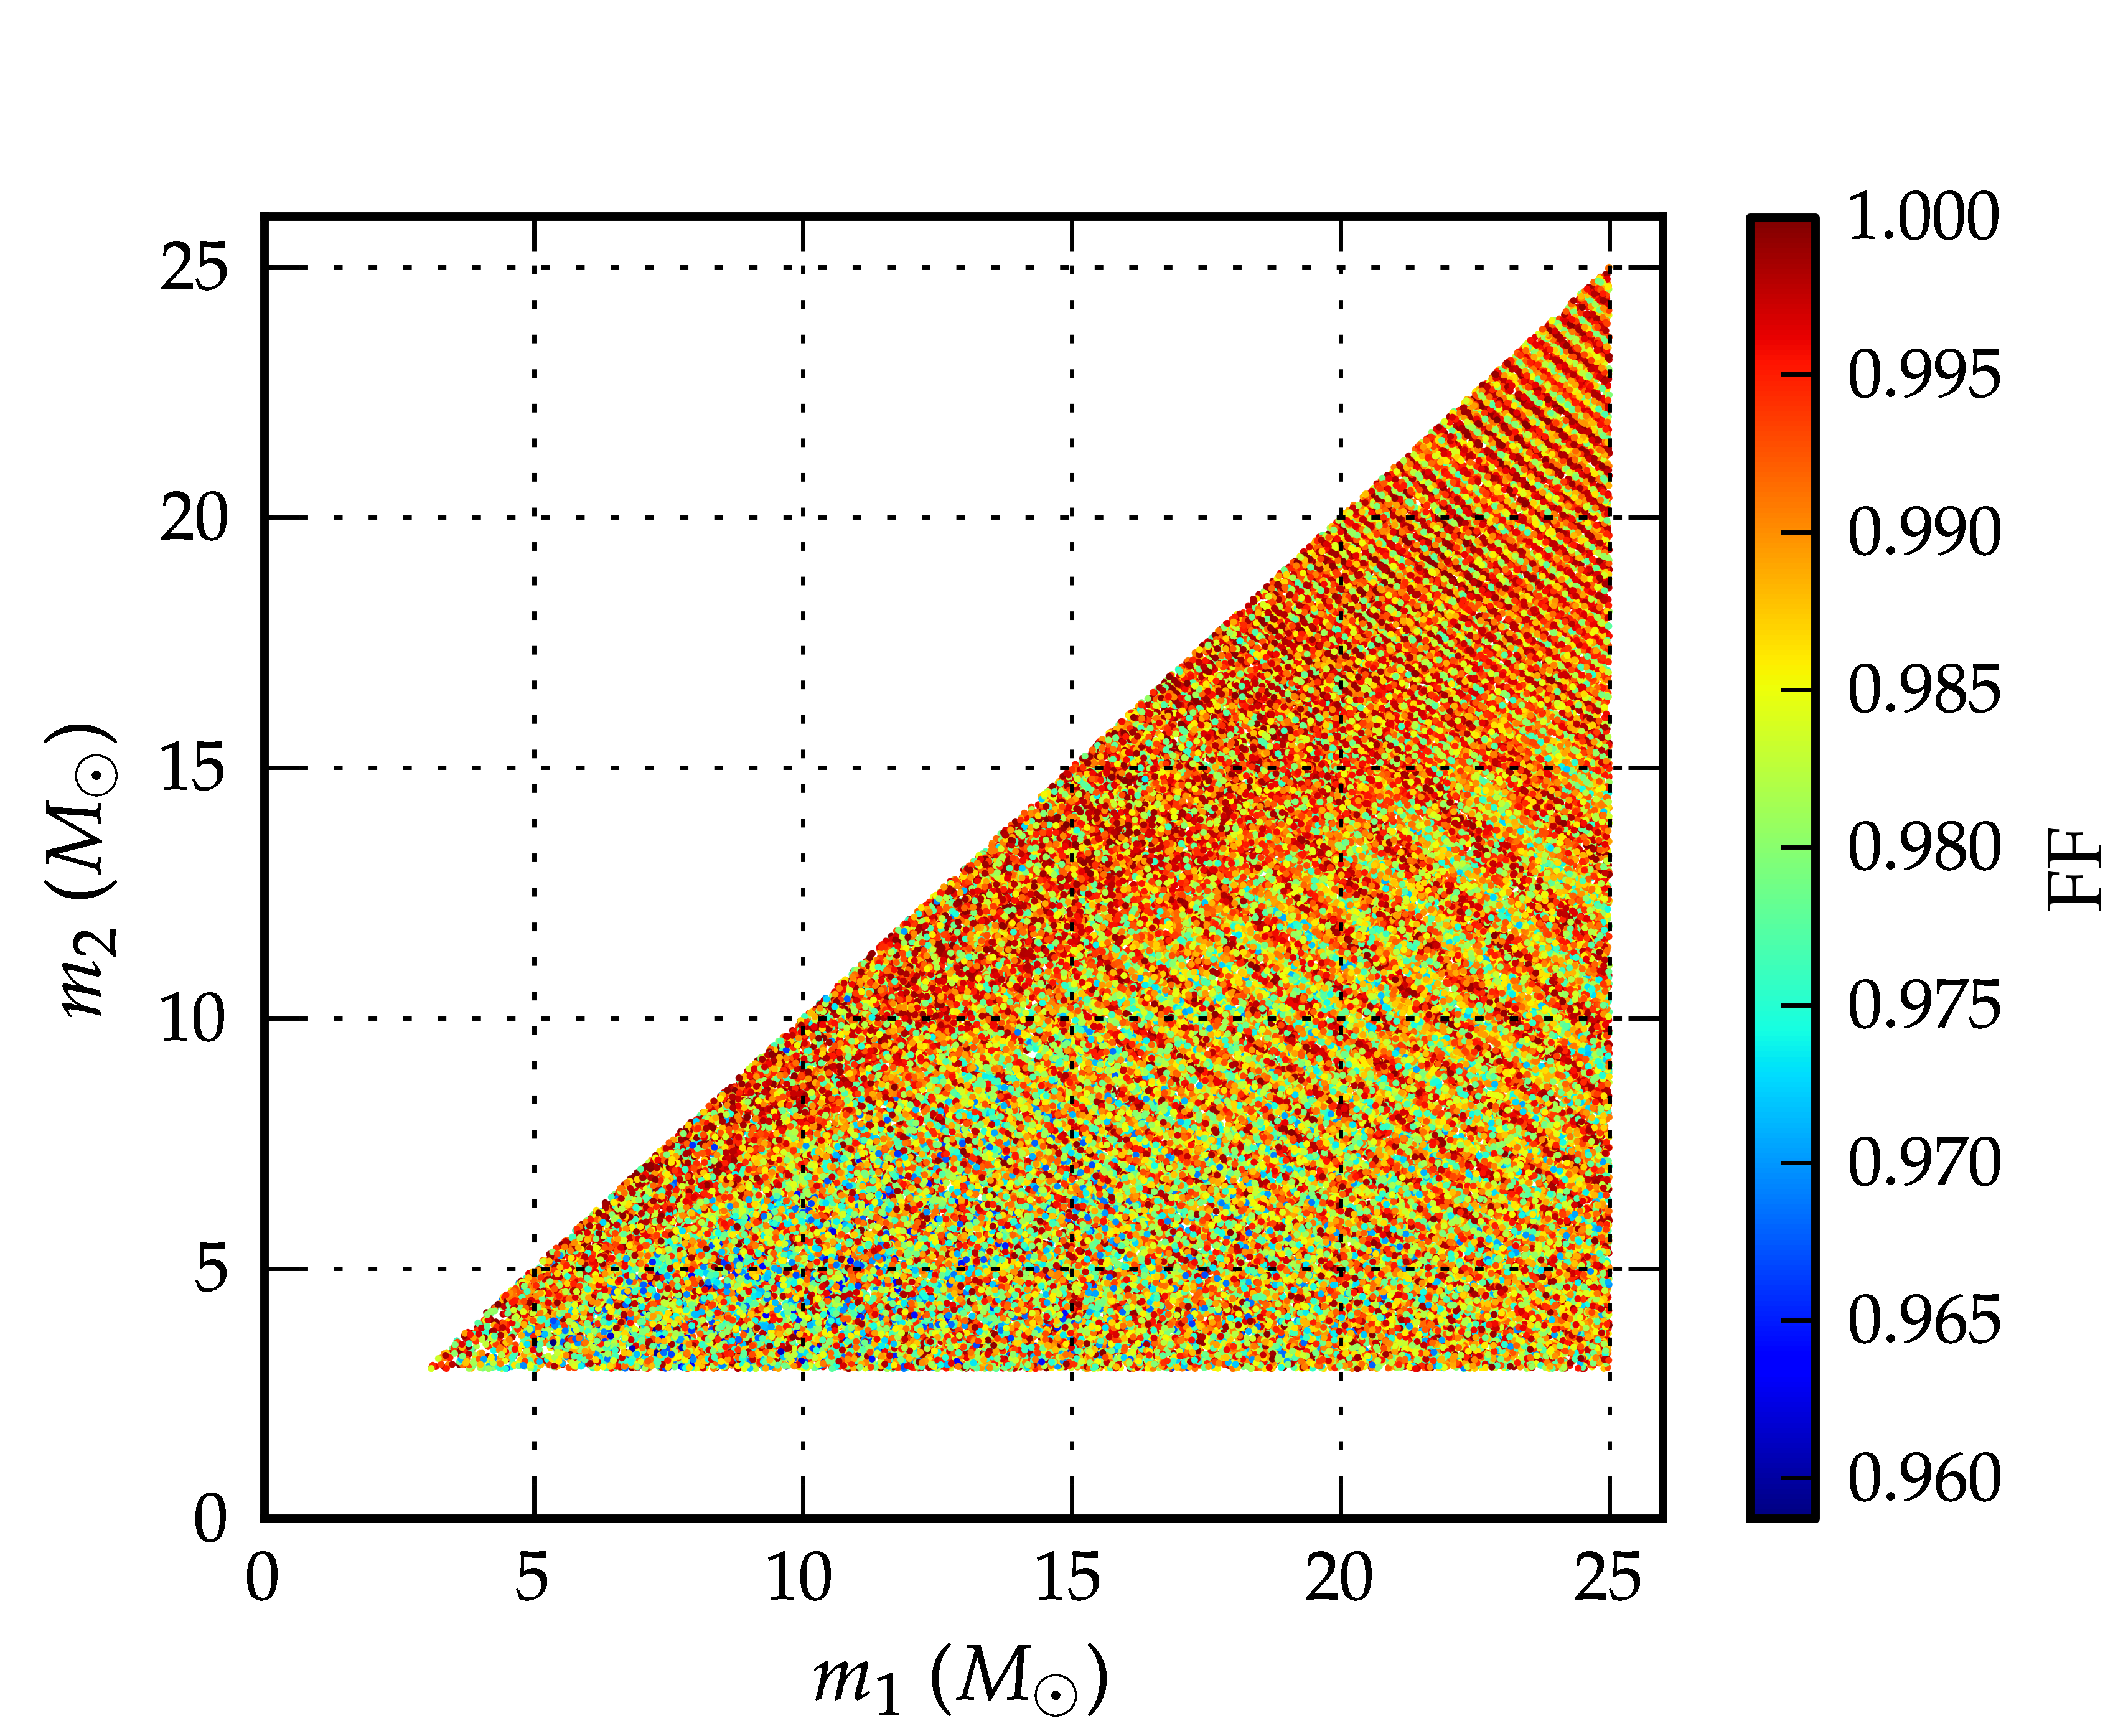
\includegraphics[width=\columnwidth]{figures/eobpnmetric/EOB22vsEOB22FULL.png}} % XXX large figure
	\end{center}
\caption{This figure shows the effectualness of a bank of EOBNRv2 templates,
placed using the 2PN accurate hexagonal template placement of
Ref.~\cite{BabaketalBankPlacement}, to search for a population of BBH signals
simulated with EOBNRv2 waveforms. The masses of the BBH population are chosen
from a uniform distribution of component masses between $3$ and $25\,
M_{\odot}$. For each injection, we plot the component masses of the injection,
and the fitting factor $\left(\FF\right)$.} \label{fig:match_eobeob_all}
\end{figure}

\begin{figure}
	\begin{center}
		\scalebox{1}{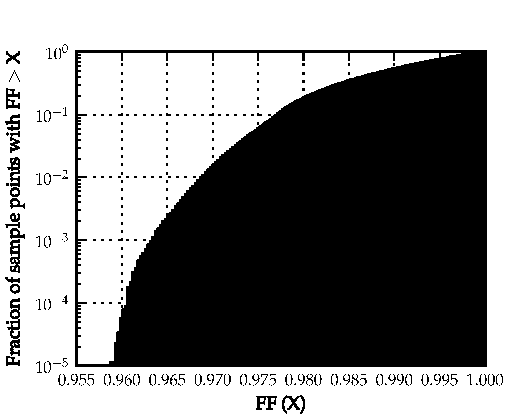
\includegraphics[clip=false, width=\columnwidth]{figures/eobpnmetric/EOB22vsEOB22FULLcumhist.pdf}}
	\end{center}
\caption{This figure shows a cumulative histogram of the fraction of the BBH
signal space (on the y-axis), where the bank of EOBNRv2 waveforms has
$\mathcal{FF}$ less than the respective values on the x-axis.  The EOBNRv2
bank has a fitting factor $\mathcal{FF}$ below the $0.97$ for less than $\sim
1.5\%$ of all simulated signals with component-masses $m_1, m_2$ between
$3\, M_\odot$ and $25\,M_{\odot}$.} \label{fig:cumhist_eobeob_all}
\end{figure} 

In this section we measure the effectualness of the second-order
post-Newtonian hexagonal template bank placement metric described in
Ref.~\cite{BabaketalBankPlacement} when used to place EOBNRv2 waveform
templates for aLIGO.  The same template placement algorithm was used to place
a grid of third-and-a-half order post-Newtonian order TaylorF2 waveforms for
low-mass BBH detection searches for initial LIGO and Virgo
observations~\cite{Colaboration:2011nz,Abadie:2010yb,Abbott:2009qj,Abbott:2009tt,Messaritaki:2005wv}.
We construct a template bank which
has a desired minimal match of $0.97$ for waveforms with component masses
between $3 M_\odot \le m_1, m_2 \le 25 M_\odot$. This template
bank contains $10,753$ template grid points in $(m_1,m_2)$ space for the aLIGO noise curve, 
compared to $373$ grid points for the initial LIGO design noise
curve. For the template waveforms at each grid point, we use the EOBNRv2
waveforms, rather than TaylorF2 waveforms.  Since the metric itself was
derived using second-order TaylorF2 waveforms, we do not, \textit{a priori}
know if this metric is a good measure to use to place template banks for
EOBNRv2 waveforms. 

To test the effectualness of this template bank, we perform a Monte-Carlo
simulation over the $3 M_\odot \le m_1, m_2 \le 25 M_\odot$ BBH mass space to
find regions where the bank placement algorithm leads to under-coverage.  We
sample 90,000 points uniformly distributed in individual component masses. For
each of these points, we generate an EOBNRv2 waveform for the system with
component masses given by the coordinates of the point.  We record the $\mathcal{FF}$ of the template
bank for each of the randomly generated BBH waveforms in the Monte-Carlo
simulation.  Since we use EOBNRv2 waveforms both to model the true BBH signals and
as matched-filter templates, any departure in fitting factor from unity is
due to the placement of the template bank grid. 

For a bank of template waveforms constructed with a $\MM$ of $0.97$,
Fig.~\ref{fig:match_eobeob_all} and Fig.~\ref{fig:cumhist_eobeob_all} show
that the $\mathcal{FF}$ of the bank remains above $0.97$ for $\sim 98.5\%$ of
all simulated BBH signals. Less than $\sim 1.5\%$ of signals have a minimal
match of less than 0.97, with the smallest value over the 90,000 sampled
points being $\sim 0.96$.  The diagonal features observed in
Fig.~\ref{fig:match_eobeob_all} are due to the hexagonal bank placement
algorithm and are related to the ellipses of constant chirp mass in Fig.~4  of
Ref.~\cite{BabaketalBankPlacement}.  From these results, we conclude that the
existing template bank placement metric adequately covers the BBH mass space
with EOBNRv2 waveform templates; it is not necessary to construct a metric
specific to the EOBNRv2 model. aLIGO detection searches can employ the
second-order post-Newtonian bank placement metric with the hexagonal placement 
algorithms~\cite{SathyaMetric2PN,SathyaBankPlacementTauN,BabaketalBankPlacement,OwenTemplateSpacing,Cokelaer:2007kx}
to place template banks for EOBNRv2
waveforms without a significant drop in the recovered signal-to-noise ratio.

\subsection{Effectualness of TaylorF2 templates}\label{s2:eob22f2}
\begin{figure}
  \begin{center}
   \scalebox{1}{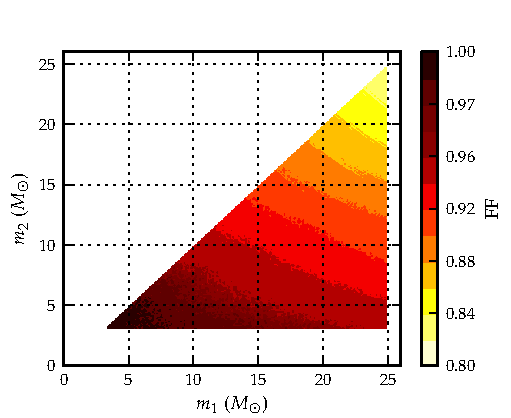
\includegraphics[width=\columnwidth]{figures/eobpnmetric/EOB22vsF2FULLNolinesContours-PRD.pdf}} 
  \end{center}
\caption{\label{fig:match_f2eob_f2eob22_all}The fitting factor $\mathcal{FF}$
of a bank of TaylorF2 waveforms, constructed with $\MM = 0.97$, 
for a population of BBH systems which are modeled using EOBNRv2 signals.} 
\end{figure}

\begin{figure}
\centering
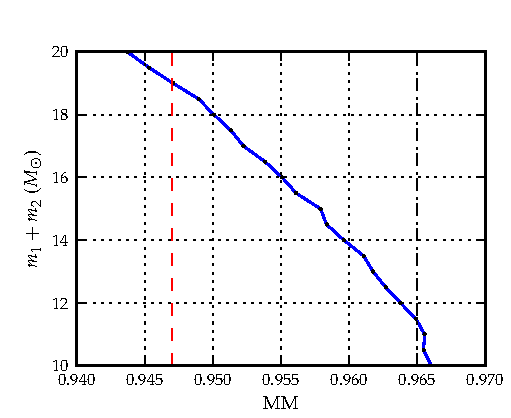
\includegraphics[scale=0.04, clip=false, keepaspectratio=true, width=\columnwidth]{figures/eobpnmetric/EOB22vsF2totalMassvsMMs-PRD.pdf} % XXX large figure

% 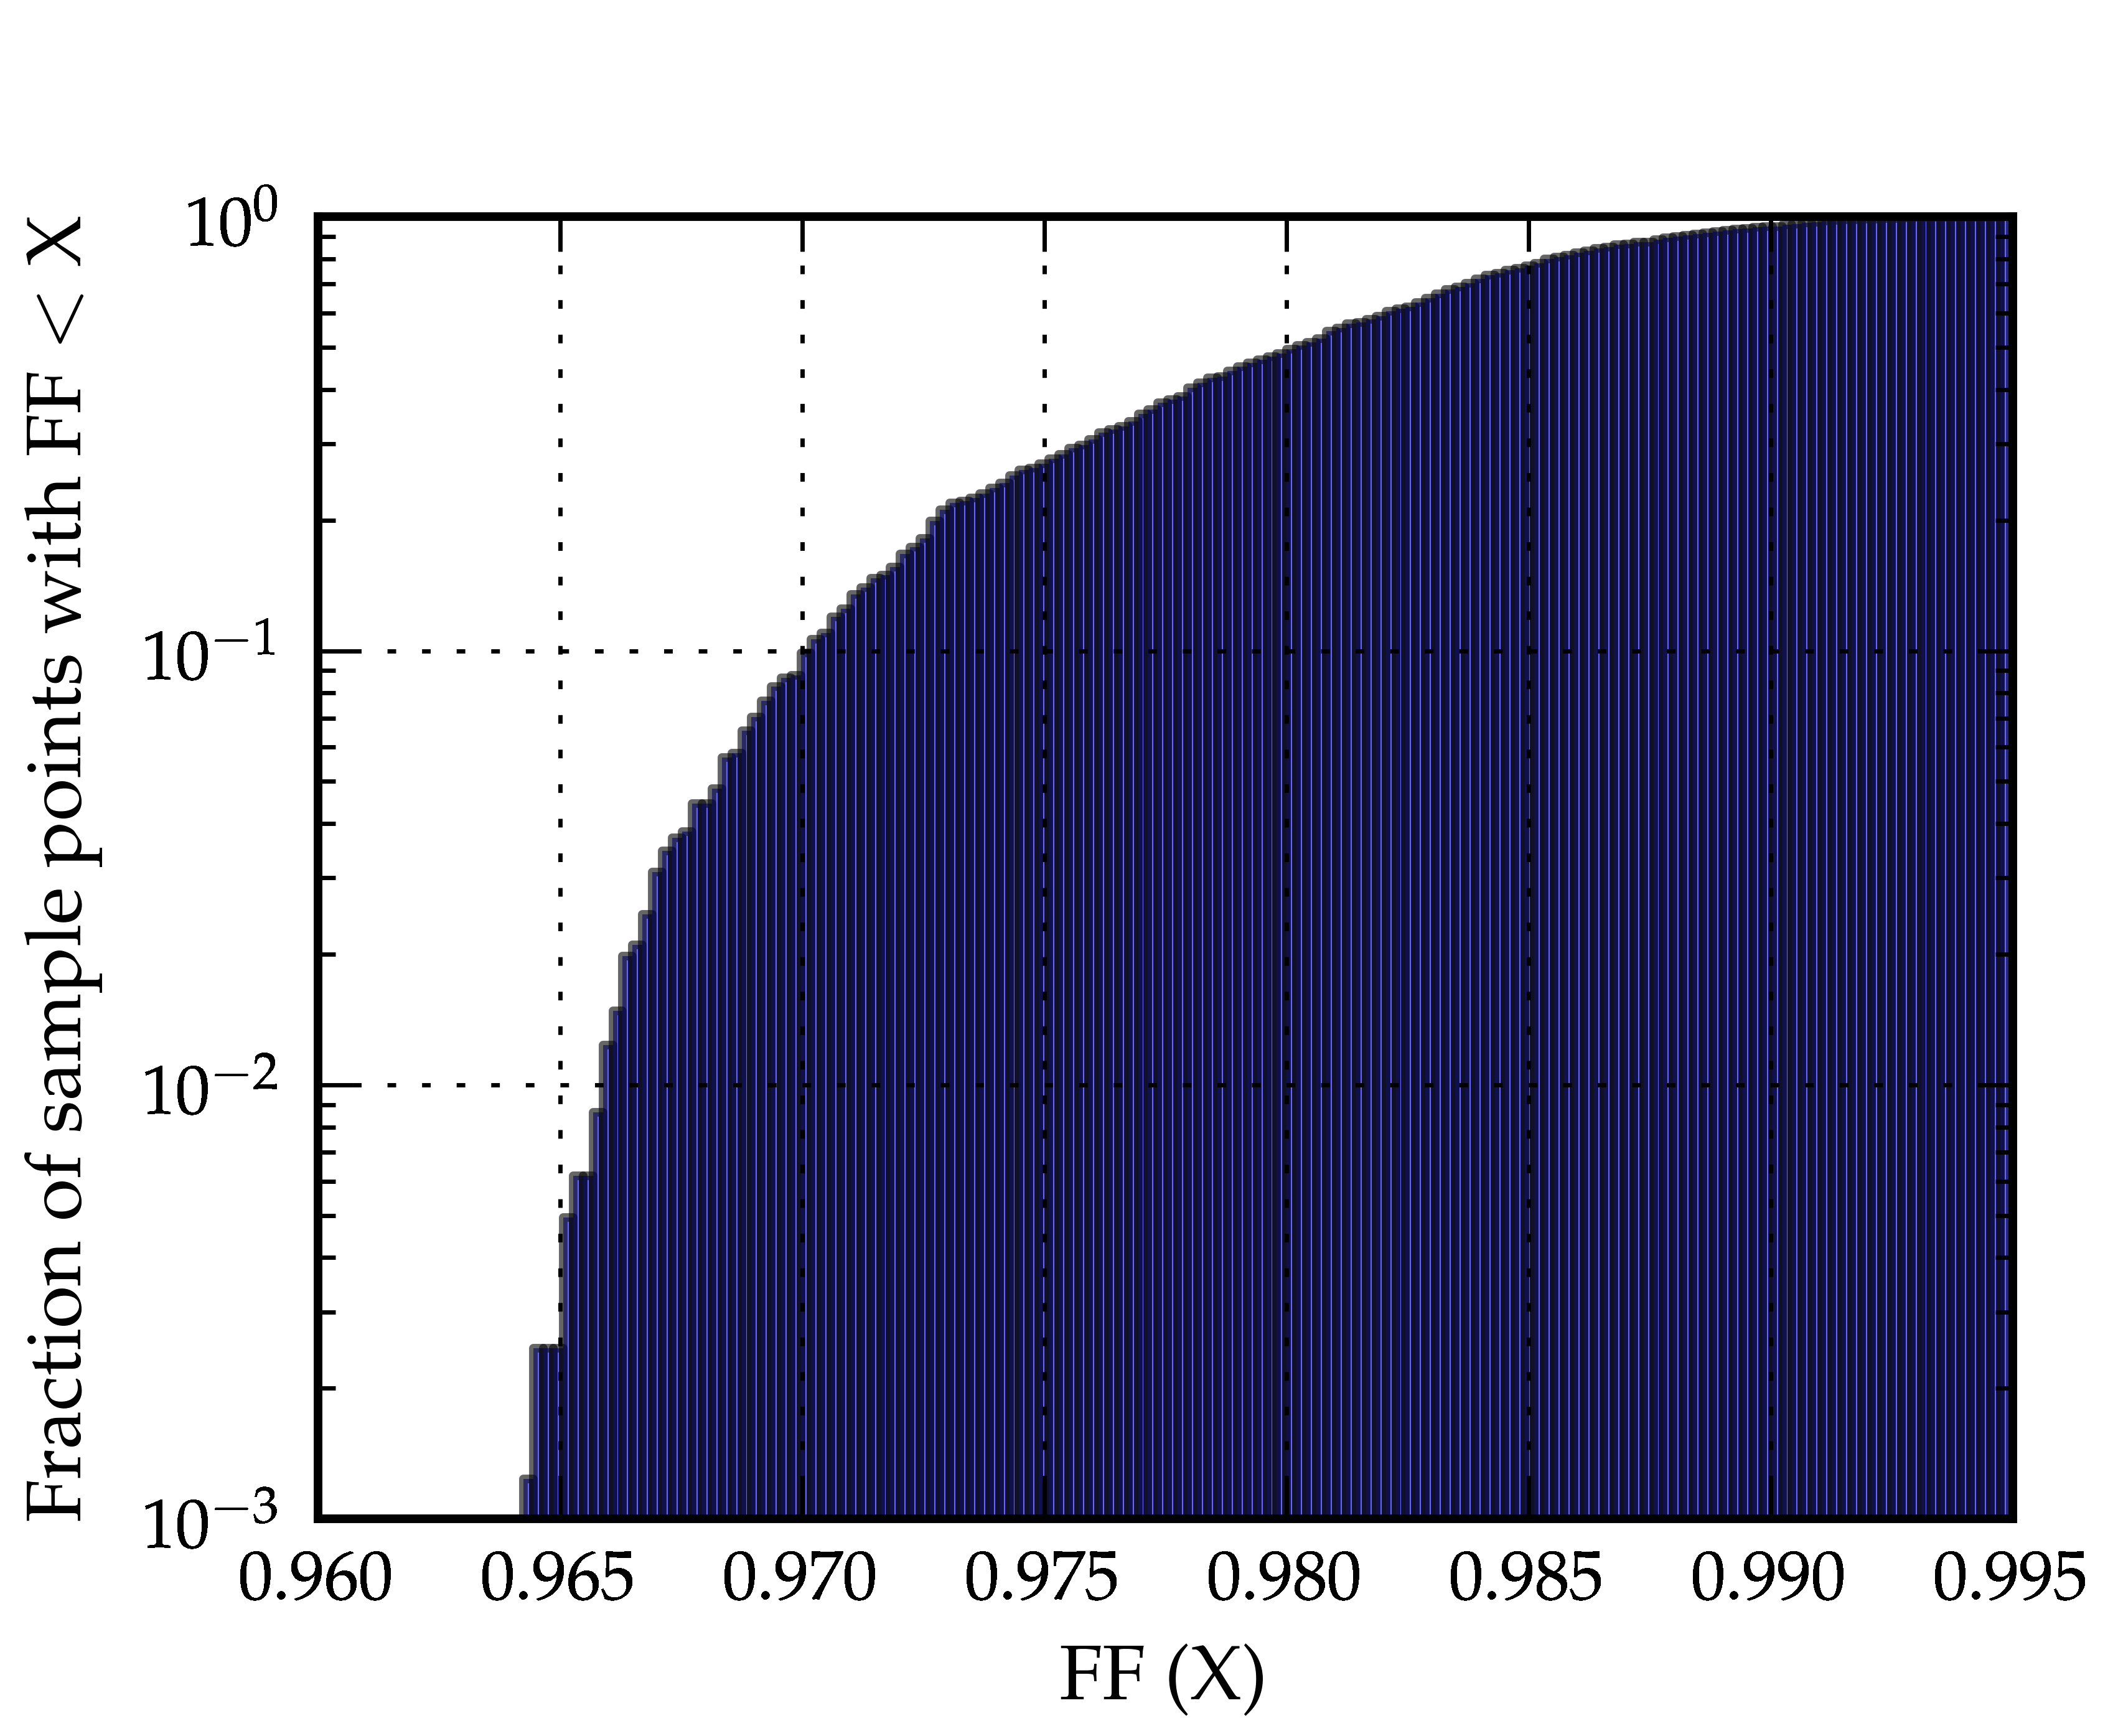
\includegraphics[scale=0.04, clip=false, totalheight=0.3\textheight, width=\columnwidth]{EOB22vsF2cutcumhist12.png}
\caption{\label{fig:mmvsM_f2eob22}The (blue) curve shows the upper-bound 
on total-mass for the sub-region over which the TaylorF2 bank has a 
minimal-fitting-factor as given on the x-axis. We observe that the TaylorF2 
bank has a minimal-fitting-factor of $0.965\,(0.947)$ for the region with total
masses below $\sim 11.4 M_{\odot}\,(19 M_{\odot})$. The minimal-fitting-factor
is the fitting-factor value which is less than the fitting-factors of the 
TaylorF2 bank for $\geq 99.75\%$ of the points sampled in the sub-region.}
\end{figure}

We next explore the efficiency of using the computationally cheaper TaylorF2
waveforms to search for a population of BBH signals with
component masses between $(3$--$25) M_\odot$. The signals from this population
are modeled 
with the full EOBNRv2 waveforms. We use the same template bank placement as above,
however now we use the third-and-a-half PN order TaylorF2 model as the
template waveforms. This model does not capture the merger and ringdown of BBH
signals, as it is terminated at the Schwarzchild test-particle ISCO.
Furthermore, it diverges from the true BBH signal in the late inspiral.
It is important to determine when these effects become important.

We sample the $(3$--$25) M_\odot$ BBH component mass space at 100,000 points by
generating an EOBNRv2 waveform to generate the ``true'' signal waveform.  We
generate a bank of TaylorF2 template waveforms over the same region, and
calculate its $\FF$ for each of the sample points, against the corresponding
EOBNRv2 waveform. Fig.~\ref{fig:match_f2eob_f2eob22_all}  shows the
distribution of the $\FF$ obtained for the TaylorF2 bank. Clearly the TaylorF2
bank is not effectual for the enture BBH region considered, with mismatches of
up to $18\%$ observed. We divide the sampled component mass space into
sub-regions which consist of systems with total masses below different thresholds,
and compute the minimal-fitting-factor of the bank over those. In Fig.~\ref{fig:mmvsM_f2eob22}, 
the blue (solid) curve shows the upper-limit on 
total mass for different sub-regions against the minimal-fitting-factor of the 
TaylorF2 bank over those. The minimal-fitting-factor over a sub-region is 
taken to be the fitting-factor value which is less than the fitting-factors
for $\geq 99.75\%$ of the points sampled in the sub-region. We find that the 
TaylorF2 template bank has $\FF$ above $0.965$ ($0.947$) for the region 
with total masses below $11.4M_{\odot}$ ($19M_{\odot}$). We conclude 
that the TaylorF2 bank is effectual for BBH signals below $\sim 11.4M_{\odot}$. 

The value of our limit on total-mass is in agreement with the previous study in
Ref.~\cite{CompTemplates2009}, however this analysis used the EOBNRv1
model~\cite{Buonanno:2007pf} and an older version of the Advanced LIGO noise
curve \cite{CompTemplates2009}. This agreement provides
confidence that this limit will be robust in aLIGO searches and we propose
this limit as the upper cutoff for the computationally cheaper TaylorF2
search. To investigate the loss in the $\FF$ due to the mismatch in the
template and signal waveform models, we also performed a Monte-Carlo
simulation using a denser TaylorF2 bank with $\MM\,=\,0.99$. We found that
using this dense bank of third-and-a-half order TaylorF2 waveforms, we can
relax the limit on the upper mass to $\sim 16.3M_{\odot}$ ($21.8M_{\odot}$) and
still achieve a  $\FF$ above $0.965$ ($0.947$), for over $99.75\%$ of the signals
sampled in the region.  However, 
increasing the minimal match increases the size of the template bank from 
$10,753$ to $29,588$ templates. This is a significant increase, compared to 
the cost of filtering with EOBNRv2 templates.

\subsection{Effect of sub-dominant modes}
\begin{figure*}
\centering
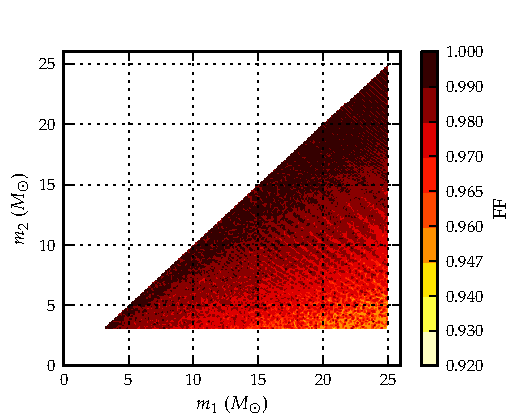
\includegraphics[scale=0.04, clip=false, totalheight=0.3\textheight, width=\columnwidth]{figures/eobpnmetric/EOBHMvsEOB22FULLNolinesContours-PRD.pdf} % XXX large figure
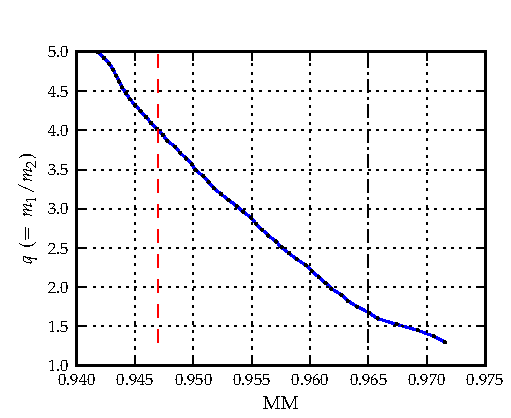
\includegraphics[scale=0.04, clip=false, totalheight=0.3\textheight, width=\columnwidth]{figures/eobpnmetric/EOBHMvsEOB22qvsMMs-PRD.pdf} % XXX large figure
% \includegraphics[scale=0.04, clip=false, totalheight=0.3\textheight, width=\columnwidth]{EOBHMvsEOB22McEtaNolines-PRD.pdf} % XXX large figure
\caption{\label{fig:match_eob22eobhm_m1m2} (left) The $\FF$ of a
bank of EOBNRv2 waveforms, constructed with a minimal match of 0.97 at each
point in the stellar-mass BBH component-mass region. While the templates are
modeled as the dominant-mode $l=m=2$ EOBNRv2 waveforms, the signals are modeled 
including the sub-dominant waveform modes as well (EOBNRv2HM). (right) This figure shows the 
upper-bound on mass-ratio ($q$) for the region where a bank of EOBNRv2
templates has a minimal-fitting-factor as given on the x-axis. We observe that for
the region with $q \leq 1.68\,(4)$, the minimum-match of the bank is below $0.965\,(0.947)$. 
From both the figures, we notice a systematic fall in the coverage of the EOBNRv2 
template bank with increasing mass-ratio.} 
\end{figure*}
\begin{figure*}
\centering
% 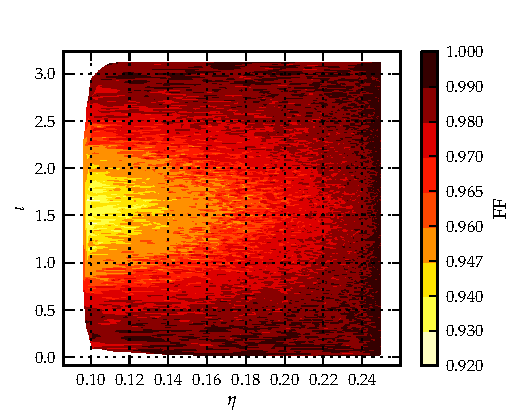
\includegraphics[scale=0.04, clip=false, width=0.67\columnwidth]{EOBHMvsEOB22incvseta-PRD.pdf} % XXX large figure
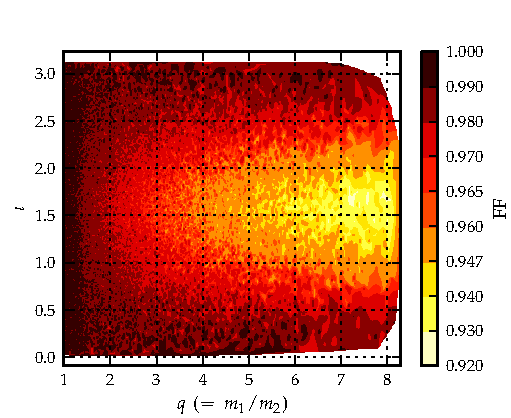
\includegraphics[scale=0.04, clip=false, totalheight=0.3\textheight, width=\columnwidth]{figures/eobpnmetric/EOBHMvsEOB22incvsq-PRD.pdf} % XXX large figure
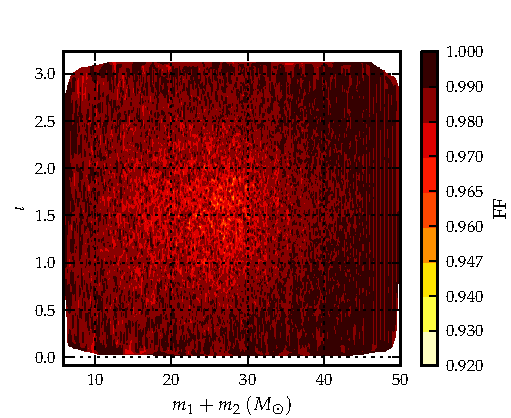
\includegraphics[scale=0.04, clip=false, totalheight=0.3\textheight, width=\columnwidth]{figures/eobpnmetric/EOBHMvsEOB22incvsM-PRD.pdf} % XXX large figure
\caption{\label{fig:incvsM_eob22eobhm} (left) The $\FF$ of a
bank of EOBNRv2 waveforms, constructed with a minimal match of 0.97 at each
point in the stellar-mass BBH $q-\iota$ space. While the templates are
modeled as the dominant-mode $l=m=2$ EOBNRv2 waveforms, the signals are modeled 
including the sub-dominant waveform modes as well (EOBNRv2HM). We observe a loss in fitting-factors, upto $\sim 8\%$, for 
systems with high mass-ratios ($q$) \textit{and} inclination angle ($\iota$) close to $\pi/2$.
(right) The $\FF$ for the same population of signals, now shown on the $M-\iota$ plane. We observe the loss in fitting factors to be relatively lesser
for more massive binaries.}
\end{figure*}
\begin{figure*}
\centering
% 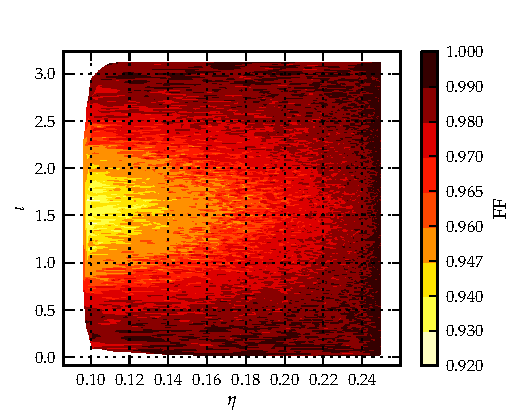
\includegraphics[scale=0.04, clip=false, width=0.67\columnwidth]{EOBHMvsEOB22incvseta-PRD.pdf} % XXX large figure
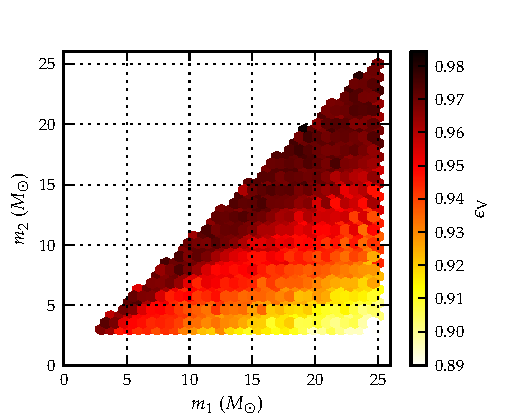
\includegraphics[scale=0.04, clip=false, totalheight=0.3\textheight, width=\columnwidth]{figures/eobpnmetric/EOBHMvsEOB22VeffLossm1m2-PRD.pdf} % XXX large figure
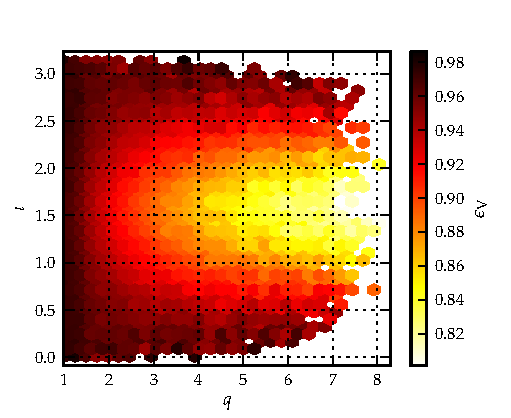
\includegraphics[scale=0.04, clip=false, totalheight=0.3\textheight, width=\columnwidth]{figures/eobpnmetric/EOBHMvsEOB22VeffLossqinc-PRD.pdf} % XXX large figure
\caption{\label{fig:VeffLoss_eob22eobhm} (left) This figure shows $\epsilon_{\mathrm{V}}\left(\theta_1=\{m_1,m_2\}\right)$ in the component-mass
space (see Eq.~\ref{eq:epsilondef}). 
This gives the 
fraction of total observable volume that is visible to a search which uses the
leading order $l=m=2$ EOBNRv2 waveform template bank, placed with the 2PN 
accurate TaylorF2 bank placement metric. For a population of signals, that is distributed uniformly in spacial volume,
this is equivalent to the fraction of the maximum possible event observation rate that we get with the use of a discrete bank of matched-filters. We observe that the loss in event observation rate,
averaged over all parameters (uniformly distributed) but $\theta_1=\{m_1,m_2\}$,
does not exceed $\sim 11\%$ for any region of the component-mass space.
(right) This figure shows $\epsilon_{\mathrm{V}}\left(\theta_1=\{q,\iota\}\right)$ over the $q-\iota$ plane. We note that the 
maximum averaged loss in the detection rate is for systems
with high mass ratios \textit{and} $\iota\in[1.08,2.02]$, and 
can go as high as $\sim 20\%$ for such systems.
} 
\end{figure*}

Having established that the second-order post-Newtonian hexagonal template
bank is effectual for placing a bank of EOBNRv2 templates, we now investigate
the effect of neglecting sub-dominant modes in BBH searches. The sensitivity
reach of the aLIGO detectors is normally computed assuming that the search is
only sensitive to the dominant $l=m=2$ mode of the gravitational waveform. For
binary black hole signals, sub-dominant modes may contain significant
power~\cite{Pekowsky:2012sr}. A search that includes these modes could, in
principle, have an increased reach (and hence event rate) compared to a search
that only uses the dominant mode. The EOBNRv2 model of
Ref.~\cite{BuonannoEOBv2Main} has been calibrated against higher order modes
from numerical relativity simulations. We investigate the effect of ignoring
these modes in a search by modeling the BBH signal as an EOBNRv2 signal
containing the dominant and sub-dominant multipoles: $h_{lm} =
h_{22},h_{21},h_{33},h_{44}, h_{55}$ (which we call EOBNRv2HM) and computing
the fitting factor of leading-order EOBNRv2 templates placed using the
TaylorF2 metric.

We simulate a population of BBH signals by sampling $100,000$ systems
uniformly in the $m_1,m_2 \in [3,25] \, M_\odot$ component-mass space. These
EOBNRv2HM signals are uniformly distributed in sky-location angles and
inclination and polarization angles, which appear in the detector's response
function to the gravitational-wave signal~\cite{Sathyaprakash:2009xs}. The 
template bank
is again placed with a desired minimal match of $0.97$ and for each of signal
waveforms, we calculate the $\FF$ against the entire bank of EOBNRv2 waveform
templates.  Fig.~\ref{fig:match_eob22eobhm_m1m2} (left panel) shows the value 
of the $\FF$
of the bank of EOBNRv2 waveform templates over the sampled component-mass 
space. As expected, the higest fitting factors are observed close to the equal mass
line, since when the mass ratio is close to unity, the amplitude of the
sub-leading waveform modes is several orders of magnitude smaller than the
amplitude of the dominant mode. As the mass ratio increases, the relative
amplitude of the sub-leading multipoles increases, as illustrated by Fig.~1 of
Ref.~\cite{BuonannoEOBv2Main} and the fitting factor decreases. This pattern
is brought out further in Fig.~\ref{fig:incvsM_eob22eobhm} (left panel),
where we show the $\FF$ values in the mass ratio - inclination angle 
($q-\iota$) plane. We
observe that when the orbital angular momentum is either parallel or anti-parallel
to the line of sight from the detector, the sub-leading multipoles do not 
contribute significantly to the signal. This is what we would expect from
Eq.~\ref{eq:hpcfromhlm}, as the spin-weighted harmonics are proportional to
$\mathrm{sin}(\dfrac{\iota}{2})\mathrm{cos}(\dfrac{\iota}{2})$, except when
$l=m=2$. Similar to Sec.~\ref{s2:eob22f2}, we divide the sampled component-mass
space into sub-regions bounded by $1\leq q \leq\,q_{\mathrm{threshold}}$, and compute
the minimal-fitting-factor of the EOBNRv2 template bank over those. In
Fig.~\ref{fig:match_eob22eobhm_m1m2} (right panel), the blue (solid) curve shows the 
value of $q_{\mathrm{threshold}}$ for each restricted sub-region against the 
minimal-fitting-factor of the bank over the same. For systems
with mass-ratio $q$ below $1.68\, (4)$, we find that the $\FF$ of the
EOBNRv2 waveform bank is above $0.965\, (0.947)$ over $99.75\%$ of this
restricted region.  These results demonstrate that
the effect of ignoring sub-dominant modes does not cause a significant loss in
the total possible signal-to-noise if the mass ratio is less than $1.68$. 
% To assess similar regions along the $\iota$-axis, We divide the sampled component-mass space 
% into sub-regions bounded by $0\leq \iota \leq \iota_{\mathrm{upper-threhold}}$ and
% $\iota_{\mathrm{lower-threhold}} \leq \iota \leq \pi$, and compute the 
% minimal-fitting-factor of the EOBNRv2 bank over those. We expect the bank to be
% effectual for systems with $\iota$ close to $0$ and $\pi$, as suggested by 
% Fig.~\ref{fig:match_eob22eobhm_m1m2} (right panel). In Fig.~\ref{fig:mmvsM_eob22eobhm}
% (right panel), the green (solid) curve shows the value of 
% $\iota_{\mathrm{lower-threhold}}$ against the minimal-fitting-factor of the bank
% over the sub-region bounded by it. 
Similar analysis over the range of possible inclination angles shows that the EOBNRv2 
waveform bank has fitting factors above $0.965\, (0.947)$ for systems with
$2.68\,(2.02)\leq \iota \leq \pi$, and $0\leq \iota \leq 0.31\,(1.08)$ (see 
Fig.~\ref{fig:incvsM_eob22eobhm}, left panel). 


Fitting factors as low as $0.92$ are observed for systems with high mass-ratios 
\textit{and} inclination angle close to $\pi/2$. As these are also binary 
configurations to which the detector is relatively less sensitive to \cite{Pekowsky:2012sr}, 
fitting-factors alone do not answer the question of where in the parameter 
space do we lose the most, in terms of detection rate. To address
this question, we compute the volume-weighted fitting-factors $\epsilon_{\mathrm{V}}$
of the EOBNRv2
template bank, over the sampled BBH parameter space. This gives us an estimate of
the expected loss in detection rate, if the source population is distributed 
uniformly in spacial volume and uniformly in intrinsic and extrinsic source parameters. 
Fig.~\ref{fig:VeffLoss_eob22eobhm} (left panel) shows $\epsilon_{\mathrm{V}}$ 
calculated in bins over the
component-mass space. In this figure, the color of each bin in the component-mass 
plane corresponds to, for a population which has all other parameters i.e. the
inclination angle and sky/polarization angles uniformly distributed over their 
possible ranges, the averaged loss in the detection rate incurred due to the use 
of a bank of leading-order $l=m=2$ EOBNRv2 templates, placed using the 2PN bank 
placement metric. We observe that
the maximum loss incurred goes up to only $\sim 10\% - 11\%$, which is within our
acceptable threshold. Looking at Fig.~\ref{fig:incvsM_eob22eobhm} (left panel), 
the maximum loss in fitting factor occurs for systems with inclination angles 
close to $\pi/2$, but (for the same mass-ratio) these
gets averaged out with systems with inclinations close to $0$ or $\pi$, which
leads to the low averaged detection-rate losses we observe in 
Fig.~\ref{fig:VeffLoss_eob22eobhm} (left panel). The right panel of 
Fig.~\ref{fig:VeffLoss_eob22eobhm} shows the same quantity, $\epsilon_{\mathrm{V}}$,
calculated over bins in the mass-ratio - inclination angle plane. As expected, 
we observe that, letting all other parameters be distributed uniformly over their
possible ranges, systems with high mass-ratios \textit{and} inclination angles 
close to $\pi/2$ will incur (averaged) losses in observation volume of 
up to $\sim 20\%$.

These results suggest that a search that includes higher order modes
could achieve a non-trivial increase in sensitivity over leading-order mode
templates, only in detecting systems with high $q$ \textit{and} $1.08\leq\iota\leq 2.02$.  
However, an algorithm that includes sub-dominant modes could have an 
increased false-alarm rate (background) over a search that includes 
only the leading-order mode, and hence the overall gain in search efficiency
might not be significant. 

\section{Conclusions}
\label{s:conclusions}

We used the TaylorF2 second-order post-Newtonian hexagonal placement algorithm
of Refs.~\cite{SathyaMetric2PN,BabaketalBankPlacement,Cokelaer:2007kx} to construct a
template bank of EOBNRv2 waveforms with $\MM$ of $0.97$. We calculated the
fitting factor ($\FF$) of this bank against $\sim 90,000$ simulated EOBNRv2
signals with component masses uniformly distributed between $3 M_{\odot} \le
m_1,m_2 \le 25 M_{\odot}$. We find that the $\FF$ of the template bank is
greater than $0.97$ for $98.5\%$ of the simulated EOBNRv2 signals, assuming
the zero-detuning high power noise spectrum for aLIGO sensitivity
\cite{aLIGONoiseCurve}. We conclude that the existing placement algorithm is
effectual for use in aLIGO BBH searches, assuming that EOBNRv2 is an accurate
model of BBH signals in this mass region.  We then demonstrated that use of the
computationally cheaper third-and-a-half order TaylorF2 waveform results in a
loss in search efficiency due to inaccuracies of the post-Newtonian
approximation, and neglect of merger-ringdown for BBHs with a total mass $M >
11.4\,M_{\odot}$. However, below this limit the TaylorF2 model is an acceptable
signal for BBH searches. This was done using a bank with a $\MM$ of 0.97. By 
increasing the density of the bank to $0.99\MM$, the limit on total-mass can be 
relaxed to $16.3\,M_{\odot}$, with an increase in computational cost due to the 
number of templates increasing by a factor of $\sim 2.7$. Finally, we investigated 
the loss in the SNR incurred by the using template banks constructed using 
only the leading order mode of EOBNRv2 waveforms.  We found that a leading-order 
$l=m=2$ EOBNRv2 template bank constructed with a $\MM$ of $0.97$ is effectual 
to search for BBHs for which $1\leq \left(m_1/m_2\right)\leq 1.68$ or $\iota \geq 2.68$ 
or $\iota\leq 0.31$ radians, and there is no significant loss in
potential signal-to-noise ratio for systems with $q$ as high as $4$ or
$2.02\leq\iota\leq 2.68$ or $0.31\leq\iota\leq 1.08$. We also observed that the
maximum loss in detection-rate, for a binary with given mass parameters, averaging
over other parameters - which are taken to be uniformly distributed over their 
possible ranges, goes only to a maximum of $\sim 10\% - 11\%$. For any given pair of 
binary masses, the loss is highest when the binary is inclined at $\simeq \pi/2$, 
and can go up to $\sim 20\%$, and is lower when its angular momentum is close to 
being parallel or anti-parallel to the line of sight from the detector. These effects 
average out, and hence for a population which is expected to have a uniform 
distribution of inclination angles (and uniform distribution in spacial volume), 
the average loss in detection rate was estimated to be not higher than $\sim 11\%$.
Thus, using EOBNRv2HM templates is unlikely to give a significant increase
in the range to which such a population of sources can be detected. For BBHs 
with $\left(m_1/m_2\right)\geq 4$ \textit{and} $1.08\leq\iota\leq 2.02$, detection searches 
could possibly gain sensitivity by the use of EOBNRv2HM waveforms, if they can be implemented 
without increasing the false alarm rate. 

Our results suggest that a significant portion of the non-spinning
stellar-mass BBH parameter space can be searched for using LIGO's existing
search algorithms. For systems with total mass below $\sim 11.4M_{\odot}$ template
banks of TaylorF2 can be used without significant loss in event rate. For
higher mass systems, neglecting high-order modes in an EOBNRv2 search does not
cause a substantial reduction in the maximum possible reach of BBH searches.
Finally, we note that our study does not consider BBH systems with BH
masses higher than $M = 25\,M_\odot$, or the effect of black hole component
spins. Future work will extend this study for systems with spinning and/or
precessing black holes and consider the effect of non-Gaussian transients in
real detector noise.



\Chapter{Binary black hole search template banks with Numerical 
Relativity waveforms}
\label{ch:NRHyb_bank}
%%%%%%%%%%%%%%%%%%%%%%%%%%%%%%%%%%%%%%%%%%%%%%%%%%%%%%%%%%%%%%%%%%%%%%%%%%%%%%%
%%% Constructing template banks with non-spinning SpEC simulations
%%%%%%%%%%%%%%%%%%%%%%%%%%%%%%%%%%%%%%%%%%%%%%%%%%%%%%%%%%%%%%%%%%%%%%%%%%%%%%%

% \section{Introduction}


% Upgrades to the LIGO and Virgo observatories are
% underway~\cite{Harry:2010zz,aVIRGO}, with first observation runs planned for
% $2015$~\cite{Aasi:2013wya}. The construction of the Japanese detector KAGRA 
% has also begun~\cite{Somiya:2011np}. The advanced detectors will be
% sensitive to gravitational waves at frequencies down to 
% $\sim 10$Hz, with an order of magnitude increase in sensitivity across the
% band. This is a significant improvement over the lower cutoff of $40$Hz
% for initial LIGO. Estimates for the expected rate of detection have
% been placed between $0.4 - 1000$ stellar-mass binary black hole (BBH)
% mergers a year~\cite{LSCCBCRates2010}. 
% The uncertainty in these estimates comes from the uncertainties in the various
% factors that govern the physical processes in the BBH formation 
% channels~\cite{1973NInfo..27...86T,1973NInfo..27...70T}. 
% In sub-solar metallicity environments, stars (in binaries) are expected to 
% lose relatively less mass to stellar winds and form more massive remnants 
% \cite{Webbink:1984ti,Kowalska:2012bb,Fryer:2011cx}. 
% Population synthesis studies estimate that sub-solar metallicity environments
% within the horizon of advanced detectors could increase the detection rates 
% to be as high
% as a few thousand per year~\cite{Dominik:2012kk,Belczynski:2012cx}. 
% On the other hand, high recoil momenta during core-collapse and 
% merger during the common-envelope phase of the binary star evolution
% could also decrease the detection 
% rates drastically~\cite{Fryer:2011cx,Dominik:2012kk}. 

% The coalescence of a BBH can be divided into three phases, (i) the 
% early-inspiral, where the component objects' motion is only mildly relativistic;
% (ii) late-inspiral and merger, where the separation between the objects becomes 
% of the order of the inner-most stable circular orbits of the component 
% black-holes and their motion becomes highly relativistic; and (iii) ringdown, 
% which involves the quasi-normal ringing of the black-hole formed from the 
% merger of the binary. The slow-motion weak-field post-Newtonian (PN) 
% approximation scheme to Einstein's field 
% equations~\cite{1938AnMat..39...65E,Einstein:1940mt,einstein1949motion}  
% accurately describes the early inspiral. In PN theory, the binary
% orbital energy and energy flux are derived as Taylor expansions in the 
% characteristic velocity of the binary $v$~\cite{Cutler:1994ys,Blanchet:2004ek,
% Blanchet:2004bb,Jaranowski:1999qd, Jaranowski:1999ye, Damour:2001bu,Droz:1999qx,
% Kidder:2007rt, Blanchet3PN}. 
% As the motion of the objects becomes more relativistic, the PN equations 
% become increasingly inaccurate, especially during the late-inspiral and 
% merger phases~\cite{CompTemplates2001,CompTemplates2009}.

GW searches so far have focused on GW bursts~\cite{Abadie:2010mt,
Abadie:2010wx,Abadie:2012rq}; coalescing compact
binaries~\cite{Colaboration:2011nz,Abadie:2010yb,Abbott:2009qj,
Abbott:2009tt,Messaritaki:2005wv,Abadie:2011kd,Aasi:2012rja},
and ringdowns of perturbed black holes~\cite{Abbott:2009km}, amongst
others~\cite{Abbott:2003yq,Abbott:2005pu,Sintes:2005fp,Abadie:2011md,
Palomba:2012wn}. For coalescing BBHs, detection searches involve 
matched-filtering~\cite{Wainstein:1962,Allen:2005fk} of the instrument
data using large banks of theoretically modeled waveform templates
as filters~\cite{Sathyaprakash:1991mt,SathyaMetric2PN,OwenTemplateSpacing,
BabaketalBankPlacement,SathyaBankPlacementTauN,Cokelaer:2007kx}.
The matched-filter is the optimal linear filter to maximize the
signal-to-noise ratio (SNR), in the presence of stochastic 
noise~\cite{1057571}. It requires an accurate modeling of the gravitational 
waveform emitted by the source binary. Early LIGO-Virgo searches 
employed template banks of Post-Newtonian (PN) inspiral 
waveforms~\cite{Colaboration:2011nz,Abadie:2010yb,Abbott:2009qj,
Abbott:2009tt,Messaritaki:2005wv}, while more recent
searches targeting high mass BBHs used complete inspiral-merger-ringdown
(IMR) waveform templates~\cite{Abadie:2011kd,Aasi:2012rja}. 

%In early LIGO-Virgo searches,
%and more recent ones targeted at low mass BBHs, the waveforms used as filters 
%were modeled within the Post-Newtonian theory~\cite{Colaboration:2011nz,
%Abadie:2010yb,Abbott:2009qj,Abbott:2009tt,Messaritaki:2005wv}. 
%For more massive binaries that merge at frequencies that LIGO was
%most sensitive to, complete inspiral-merger-ringdown (IMR) waveforms
%were used, during the LIGO-Virgo observation period
%from 2005-07 and 2009-10~\cite{Abadie:2011kd,Aasi:2012rja}. 

Recent developments in Numerical Relativity (NR) have provided complete 
simulations of BBH dynamics in the strong-field regime, i.e. during the
late-inspiral and merger phases~\cite{Pretorius2005,Baker:2005vv,Campanelli:2005dd,
Pretorius2006,Lindblom:2005qh}. These simulations have contributed 
unprecedented physical insights to the understanding of BBH mergers
%, like black hole recoil due to 
%asymmetric emission of gravitational radiation~\cite{Herrmann:2006ks,
%Baker:2006vn,Herrmann:2007ac,Koppitz:2007ev,Campanelli:2007ew,Gonzalez:2007hi,
%Campanelli:2007cga,Baker:2007gi,Herrmann:2007ex,Brugmann:2007zj,
%Schnittman:2007ij,Pollney:2007ss,Healy:2008js,Gonzalez:2008bi},
%and prediction of the physical parameters of the Kerr black hole 
%remnant~\cite{Campanelli:2006fg,Campanelli:2006fy,Rezzolla:2007xa,
%Boyle:2007sz,Rezzolla:2007rd,Marronetti:2007wz,Rezzolla:2008sd,Lousto:2009mf,
%Hemberger:2013hsa}.
(see, e.g., ~\cite{Pretorius:2007nq,Hannam:2009rd,Hinder:2010vn,Pfeiffer:2012pc} 
for recent overviews of the field).
Due to their high computational cost, fully numerical simulations currently 
span a few tens of inspiral orbits before merger. For mass-ratios
$q=m_{1}/m_{2}=1,2,3,4,6,8$, the multi-domain Spectral Einstein code 
(SpEC)~\cite{spec} has been used to simulate 15--33 inspiral merger 
orbits~\cite{Buchman:2012dw,Mroue:2012kv,Mroue:2013xna}.
These simulations have been used to calibrate waveform models, for example,
within the effective-one-body (EOB) formalism~\cite{EOBOriginalBuonannoDamour,
EOBNRdevel01,BuonannoEOBv2Main,Taracchini:2012ig}. 
Alternately, inspiral waveforms from PN theory can be
joined to numerical BBH inspiral and merger waveforms, to construct longer 
\textit{hybrid} waveforms~\cite{Boyle:2011dy,MacDonald:2011ne,MacDonald:2012mp,
Ohme:2011zm,Hannam:2010ky}. NR-PN hybrids have been used to calibrate 
phenomenological waveform models~\cite{Ajith:2007qp,Santamaria:2010yb},
%,Huerta:2012zy
and within the NINJA project~\cite{Aylott:2009tn,Ajith:2012tt}
to study the efficacy of various GW search algorithms towards realistic (NR)
signals~\cite{Santamaria:2009tm,Aylott:2009ya}.

Constructing template banks for gravitational wave searches has
been a long sought goal for NR. Traditionally, intermediary waveform
models are calibrated against numerical simulations and then
used in template banks for LIGO searches~\cite{Abadie:2011kd,
Aasi:2012rja}. In this chapter we explore an alternative to this
traditional approach, proposing the use of NR waveforms themselves
and hybrids constructed out of them as search templates.
For a proof of principle, we focus on the non-spinning BBH space, 
with the aim of extending to spinning binaries in future work. We
investigate exactly where in the mass space can the existing NR 
waveforms/hybrids be used as templates, finding that only six 
simulations are sufficient to cover binaries with 
$m_{1,2}\gtrsim 12M_\odot$ upto mass-ratio $10$. This method can
also be used as a guide for the placement of parameters for future
NR simulations. Recent work has shown that existing PN waveforms 
are sufficient for aLIGO searches for 
$M=m_1+m_2\lesssim 12M_\odot$~\cite{CompTemplates2009,Brown:2012nn}.
To extend the NR/hybrid bank coverage down to 
$M\simeq 12M_\odot$, we demonstrate that a total of $26$ 
simulations would be sufficient. The template banks are 
constructed with the requirement that the net SNR recovered for 
any BBH signal should remain above $96.5\%$ of its optimal value.
Enforcing this tells us that these $26$ simulations would be 
required to be $\sim 50$ orbits long. This goal is achievable,
given the recent progress in simulation 
technology~\cite{MacDonald:2012mp,Mroue:2013xna,BelaLongSimulation}. 
Our template banks are viable for GW searches with aLIGO, and the 
framework for using hybrids within the LIGO-Virgo software 
framework has been demonstrated in the NINJA-2
collaboration~\cite{NINJA2:2013inPrep}. In this chapter, we also 
derive waveform modeling error bounds which are independent of
analytical models. These can be extended straightforwardly to 
assess the accuracy of such models.

% This work can also be extended to quantify the errors of analytic
% and phenomenological waveform models. 

% IMR waveform models, such as the EOB and phenomenological models, 
% build on resummed or phenomenological extensions of results from PN 
% theory. The free parameters in the models are fitted to extend them
% to arbitrary values of physical paraemters. This is done by requiring
% agreement with a sample of NR waveforms that cover a few tens
% of inspiral cycles before merger. Their intrinsic modeling errors
% for the late-inspiral phase, however, are difficult to quantify 
% precisely, especially for mass (and spin) values to which the models 
% are interpolated or extrapolated to. On the other hand, we have 
% hybrid waveforms that are available for a restricted set of 
% binary masses and spins. Their intrinsic errors arise out of the
% yet-unknown higher order PN terms, which become significant as the 
% characteristic velocity increases. We can put a (conservative) 
% quantitative bound on these~\cite{MacDonald:2011ne,MacDonald:2012mp}.
% This allows us to consider the effect of template modeling errors
% on the SNR recovery of matched-filtering searches, which could be
% significant for stellar mass BBHs.
% 
% Therefore we propose the use of purely-NR and NR-PN hybrid waveforms
% as templates in GW searches with aLIGO. In this chapter, we demonstrate
% the feasibility of doing so for non-spinning BBHs, with the aim of 
% extending the method to spinning binaries in future work. We find 
% that the currently available hybrids are sufficient to cover a 
% significant portion of the binary masses, including BBHs with 
% component masses above $12M_\odot$. 
% It has been a long standing aim of Numerical Relativity to provide
% simulations that can be directly applied to GW searches. We show that
% aiming at a complete hybrid template bank is useful in choosing the
% physical parameters for future NR simulations. Towards this aim, we 
% give the set of mass-ratios for which NR simulations would be required,
% and sufficient, for complete non-spinning hybrid banks for aLIGO.
% The detectory sensitivity is modeled using the final design zero-detuning
% high-power noise curve~\cite{aLIGONoiseCurve,aLIGOsensitivity}, with
% filtering starting at $15$~Hz.


First, we construct a bank for purely-NR templates, restricting to
currently available simulations~\cite{MacDonald:2012mp,Mroue:2012kv,
Buchman:2012dw,Mroue:2013xna,Mroue:2012kv}. We use a stochastic algorithm 
similar to Ref.~\cite{Harry:2009ea,Ajith:2012mn,Manca:2009xw}, 
and place a template bank grid
constrained to $q=m_1/m_2=\{1,2,3,4,6,8\}$. The bank placement 
algorithm uses the EOB model from Ref.~\cite{BuonannoEOBv2Main} (EOBNRv2).
As this model was calibrated against NR for most of these mass-ratios, 
we expect the manifold of EOBNRv2 to be a reasonable approximation 
for the NR manifold. In Sec.~\ref{s1:NRpNhybridbank}, we demonstrate that
this approximation holds well for NR-PN hybrids as well.
To demonstrate the efficacy of the 
bank, we measure its fitting-factors (FFs)~\cite{FittingFactorApostolatos} over
the BBH mass space. We simulate a population of $100,000$ BBH waveforms with
masses sampled uniformly over 
$3M_\odot\leq m_{1,2}\leq 200M_\odot$ and $M=m_1+m_2\leq 200M_\odot$, and filter
them through the template bank to characterize its SNR recovery. For a
bank of NR templates, any SNR loss accrued will be due to the coarseness
of the bank grid. We measure this requiring both signals and templates
to be in the same manifold, using the EOBNRv2 model for both. We find 
that for systems with chirp mass 
$\mathcal{M}_c \equiv (m_1 + m_2)^{-1/5} (m_1 m_2)^{3/5}$ above 
$\sim 27M_{\odot}$ and $1\leq q\leq 10$, this bank has FFs $\geq 97\%$ and
is sufficiently accurate to be used in GW searches.
We also show that the coverage of the purely-NR bank can be extended to
include $10\leq q\leq 11$, if we instead constrain it to templates with
mass-ratios $q=\{1,2,3,4,6,9.2\}$.

Second, we demonstrate that currently available PN-NR hybrid waveforms can be 
used as templates to search for BBHs with much lower masses. The hybrids
used correspond to mass-ratios $q=\{1,2,3,4,6,8\}$. We use two distinct methods
of bank placement to construct a bank with these mass-ratios, and compare the
two. The first method is the stochastic algorithm we use for purely-NR 
templates. The second is a deterministic algorithm, that constructs the 
two-dimensional bank (in $M$ and $q$) through a union of six one-dimensional
banks, placed separately for each allowed value of mass-ratio. Templates are
placed over the total mass dimension by requiring that all pairs of neighboring
templates have the same noise weighted overlap. As before, we measure the SNR 
loss from both banks, due to the discrete placement of the templates, by 
simulating a population of $100,000$ BBH signals, to find the SNR recovered.
We measure the intrinsic hybrid errors using the method of
Ref.~\cite{MacDonald:2011ne,MacDonald:2012mp}, and subsequently account for 
them in the SNR recovery fraction. We find that the NR-PN
hybrid bank is effectual for detecting BBHs with $m_{1,2}\geq 12M_{\odot}$, 
with FFs $\geq 96.5\%$. The number of templates required was found
to be close to that of a bank constructed using the second-order TaylorF2
hexagonal bank placement algorithm~\cite{Sathyaprakash:1991mt,SathyaMetric2PN,
OwenTemplateSpacing,BabaketalBankPlacement,
SathyaBankPlacementTauN,Cokelaer:2007kx}. We note that by pre-generating the
template for the least massive binary for each of the mass-ratios that 
contribute to the bank, we can re-scale it on-the-fly to different total 
masses in the frequency domain~\cite{Sathyaprakash:2000qx}. 
Used in detection searches, such a bank would be computationally inexpensive 
to generate relative to a bank of time-domain modeled waveforms.

Finally, we determine the minimal set of NR simulations that we would need to 
extend the bank down to $M\simeq 12M_\odot$. We find that a bank that
samples from the set of $26$ mass-ratios listed in Table~\ref{table:fullqlist}
would be sufficiently dense, even at the lowest masses, for binaries with 
mass-ratios $1\leq q\leq 10$. We show that this bank recovers more than
$98\%$ of the optimal SNR, not accounting for hybrid errors. 
To restrict the loss in event detection 
rate below $10\%$, we restrict the total SNR loss below $3.5\%$. 
This implies the hybrid error mismatches stay below $1.5\%$, which 
constrains the length of the NR part for each hybrid.
We find that NR simulations spanning about $50$ orbits of late-inspiral, merger
and ringdown would suffice to reduce the PN truncation error to the desired 
level. With such a bank of NR-PN hybrids and purely-PN templates for lower
masses, we can construct GW searches for stellar-mass BBHs with mass-ratios 
$q\leq 10$.

The chapter is organized as follows, in Sec.~\ref{s2:NRwaveforms}, we discuss
the NR waveforms used in this study, in Sec.~\ref{s2:PNwaveforms} we
describe the PN models used to construct the NR-PN hybrids,  and in Sec.~\ref{s2:NRpNhybridwaveforms} we describe the
construction of hybrid waveforms. In Sec.~\ref{s2:EOBwaveforms} we 
describe the EOB model that we use to place and test the template
banks. In Sec.~\ref{s1:quantifyingerrors} we describe the accuracy
measures used in quantifying the loss in signal-to-noise ratio in a
matched-filtering search when using a discrete bank of templates and
in the construction of hybrid waveforms. In Sec.~\ref{s1:NRonlybank}
we describe the construction and efficacy of the NR-only banks, while in
Sec.~\ref{s1:NRpNhybridbank} we discuss the same for the NR-PN hybrid 
template banks constructed with currently available NR waveforms. In
Sec.~\ref{s1:futureNRpNhybridbank}, we investigate the parameter and length
requirements for future NR simulations in order to cover the entire 
non-spinning parameter space with $12 M_\odot\leq M\leq 200M_\odot$, 
$m_{1,2} \geq 3M_\odot$, and $1 \leq q \leq 10$. Finally, in 
Sec.~\ref{s1:conclusions} we summarize the results. 

\section{Waveforms}\label{s1:waveforms}

In the sections that follow, we will describe the construction of template 
banks for NR or NR-PN hybrid waveform templates. The NR waveforms that we
use correspond to mass ratios $q=\{1,2,3,4,6,8\}$, and were simulated using
the SpEC code~\cite{spec}. The construction of hybrid
waveforms involves joining a long inspiral portion, modeled using PN theory,
to the merger-ringdown waveform from NR. In this section we describe both, the 
NR waveforms and the PN models used in our study. Measuring the effectualness
of these banks involves simulating a population of BBH signals. We use the 
recently published EOBNRv2 model~\cite{BuonannoEOBv2Main} to obtain waveforms
for BBHs with arbitrary masses. This model was calibrated against five out of 
the six NR simulations we use to construct our banks, and is expected to be 
faithful at comparable mass ratios~\cite{BuonannoEOBv2Main}. In this section, 
we briefly summarize the construction of EOBNRv2 waveforms as well.

%%%%%%%%%%%%%%%%%%%%%%%%%%%%%%%%%%%%%%%%%%%%%%%%%%%%%%%%%%%%%%%%
\subsection{Numerical Relativity simulations}\label{s2:NRwaveforms}

The numerical relativity waveforms used in this chapter were produced
with the SpEC code~\cite{spec}, a multi-domain pseudospectral code to solve
Einstein's equations. SpEC uses Generalized Harmonic coordinates,
spectral methods, and a flexible domain decomposition, all of which
contribute to it being one of the most accurate and efficient codes
for computing the gravitational waves from binary black hole
systems. High accuracy numerical simulations of the late-inspiral,
merger and ringdown  of coalescing binary black-holes have been
recently performed for mass-ratios $q\equiv m_1/m_2\in\{1,2,3,4,6,8\}$
~\cite{Buchman:2012dw,Scheel:2008rj,NRPNComparisonBoyleetal,Mroue:2012kv}.

The equal-mass,
non-spinning waveform covers 33 inspiral orbits and was first discussed
in~\cite{MacDonald:2012mp,Mroue:2012kv}. 
This waveform was obtained with numerical techniques similar to those 
of~\cite{Buchman:2012dw}. The unequal-mass waveforms of mass ratios 
$2, 3, 4,$ and $6$ were presented in detail in Ref.~\cite{Buchman:2012dw}.
The simulation with mass ratio $6$ covers about 20 orbits and the
simulations with mass ratios 2, 3, and 4 are somewhat shorter and
cover about 15 orbits. The unequal mass waveform with mass ratio 8 was
presented as part of the large waveform catalog
in~\cite{Mroue:2013xna,Mroue:2012kv}. It is approximately 25 orbits in
length. 
% As it becomes possible to simulate BBH evolution for longer times, in our 
% template bank construction we assume that simulations that span $\gtrsim 20$
% orbits, including the inspiral, merger and ringdown cycles, are (will be) 
% available by the time Advanced LIGO begins observation runs. 
We summarize the NR simulations used in this study in 
Table~\ref{table:etalist4}. In the table, we also give the  
lowest total masses for which the NR waveforms span the aLIGO 
band, starting at $15$~Hz.

\begin{table}
\begin{tabular}{| c | c | c | c |}
\hline
$\hspace{10pt}\eta\hspace{10pt}$ & \hspace{15pt} q\hspace{15pt} & Length (in orbits) & Minimum total mass ($M_\odot$)\\ \hline
0.25 & 1 & 33 & 49 \\
0.2222 & 2 & 15 & 76 \\
0.1875 & 3 & 18 & 82 \\
0.1600 & 4 & 15 & 87 \\
0.1224 & 6 & 20 & 83 \\
0.0988 & 8 & 25 & 83 \\
%0.0884 & 9.2 & ?? \\
\hline
\end{tabular}
\caption{SpEC BBH simulations used in this study.  Given are symmetric mass-ratio $\eta$, mass-ratio $q=m_1/m_2$, and the length in orbits of the simulation. 
The last column gives the lowest total masses for which the NR simulations 
cover the entire coalescence process within the sensitive band of aLIGO,
starting at $15$~Hz.}
\label{table:etalist4}
\end{table}

\subsection{Post-Newtonian waveforms}\label{s2:PNwaveforms}

We make use of the Taylor\{T1,T2,T3,T4\} flavors of the post-Newtonian 
approximant family to construct hybrid waveforms. 
The construction of these models is described in 
Sec.~\ref{sec:PNWaveforms} and explicit expressions for the phasing and 
amplitudes are detailed in Appendix~\ref{sec:PNAppendix}. 
Construction of hybrid waveforms is described in the following section.

% Post-Newtonian (PN) theory is a perturbative approach to describing the
% motion of a compact object binary, during the slow-motion and weak-field 
% regime, i.e. the inspiral phase. The conserved energy of a binary in orbit,
% $E$, has been calculated to 3PN order in literature~\cite{Jaranowski:1997ky,
% Jaranowski:1999ye,Jaranowski:1999qd,Damour:2001bu,Blanchet:2003gy,
% Damour:2000ni,Blanchet:2002mb}.
% Using the adiabatic approximation, we treat the course of inspiral as a series
% of radially shrinking circular orbits. This is valid during the inspiral when
% the angular velocity of the binary evolves more slowly than the orbital 
% time-scale. The radial separation shrinks as the binary loses energy to 
% gravitational radiation that propagates outwards from the system. 
% % For a binary with individual component masses $m_1$ and $m_2$ and total mass
% %$M=m_1+m_2$, the conserved energy accurate to 3PN
% % can be written as \cite{Jaranowski:1997ky,Jaranowski:1999ye,Jaranowski:1999qd,Damour:2001bu,Blanchet:2003gy,Damour:2000ni,Blanchet:2002mb}
% % \begin{equation}
% % \begin{split}\label{eq:E3PN}
% % E_3(v)=&-\dfrac{1}{2}\eta v^2 \left[1- \l(\dfrac{3}{4}+\dfrac{1}{12}\eta\r)v^2 - \l(\dfrac{27}{8}-\dfrac{19}{8}\eta\right.\right.\\
% % +&\left.\left.\dfrac{1}{24}\eta^2 \r)v^4 - \l(\dfrac{675}{64}-\l(\dfrac{34445}{576}-\dfrac{205}{96}\pi^2\r)\eta\right.\right.\\
% % +&\left.\left.\dfrac{155}{96}\eta^2 +\dfrac{35}{5184}\eta^3\r) v^6\right],
% % \end{split}
% % \end{equation}
% % where $\eta=m_1m_2/(m_1+m_2)^2$, $v=(\pi Mf)^{1/3}$ is the characteristic velocity of the binary, and $f$ denotes the frequency of the emitted gravitational wave throughout.
% The energy flux from a binary $F$ is known in PN theory to 3.5PN 
% order~\cite{FluxandE3-5PN,Blanchet:2004ek,Blanchet:2005tk,Blanchet:2004bb}.
% % \begin{equation}
% % \begin{split}\label{eq:Ft3.5PN}
% % F_{3.5}(v)=&\dfrac{32}{5}\eta^2 v^{10}\left[1 - \l(\dfrac{1247}{336}+\dfrac{35}{12}\eta\r)v^2+4\pi v^3\right.\\
% % -&\left.\l(\dfrac{44711}{9072}-\dfrac{9271}{504}\eta -\dfrac{65}{18}\eta^2 \r)v^4\right.\\
% % -&\left.\l(\dfrac{8191}{672}+\dfrac{583}{24}\eta\r)\pi v^5+ \l(\dfrac{6643739519}{69854400}\right.\right.\\
% % +&\left.\left.\dfrac{16}{3}\pi^2 -\dfrac{1712}{105}\gamma +\l(\dfrac{41}{48}\pi^2 -\dfrac{134543}{7776}\r)\eta \right.\right.\\
% % -&\left.\left.\dfrac{94403}{3024}\eta^2 -\dfrac{775}{324}\eta^3 -\dfrac{856}{105}\textrm{log}(16v^2)\r)v^6\right.\\ 
% % -&\left.\l(\dfrac{16285}{504}-\dfrac{214745}{1728}\eta -\dfrac{193385}{3024}\eta^2 \r)\pi v^7\right],
% % \end{split}
% % \end{equation}
% % where $\gamma$ is Euler's constant. In the limit $\dot{\omega}/\omega \ll 1$, 
% % we can approximate the energy of the system to be the energy averaged over a 
% % period. 
% Combining the energy balance equation, $\D E/\D t = -F$, with Kepler's law 
% gives a description of the radial and orbital phase evolution of the binary. 
% We start the waveform where the GW frequency enters the sensitive frequency 
% band of advanced LIGO, i.e. at $15$Hz. 
% % \begin{subequations}\label{eq:PNOrbitalEvolution01}
% % \begin{align}
% % \dfrac{\D\phi}{\D t} - \dfrac{v^3}{M} &= 0,\label{eq:PNOrbitalEvolution01_01}\\
% % \dfrac{\D v}{\D t} + \dfrac{F(v)}{M\l(\D E/\D v\r)} &= 0.\label{eq:PNOrbitalEvolution01_02}
% % \end{align}
% % \end{subequations}
% Depending on the way the expressions for orbital energy and flux
% %in Eq.~\ref{eq:E3PN} \& \ref{eq:Ft3.5PN} 
% are combined to obtain the coordinate evolution for the binary,
% %to solve Eq.~\ref{eq:PNOrbitalEvolution01}, 
% we get different Taylor\{T1,T2,T3,T4\} time-domain approximants. Using the 
% stationary phase approximation~\cite{MatthewsWalker}, frequency-domain 
% equivalents of these approximants, i.e. TaylorF$n$, can be constructed. 
% Past GW searches have extensively used the TaylorF2 approximant, as it has a
% closed form and mitigates the computational cost of generating and numerically
% fourier-transforming time-domain template~\cite{Colaboration:2011nz,Abadie:2010yb,
% Abbott:2009qj,Abbott:2009tt,Messaritaki:2005wv}.
% We refer the reader to Ref.~\cite{PNtheoryLivingReviewBlanchet,JolienGWPhysAst}
% for an overview.
% From the coordinate evolution, we obtain the emitted gravitational waveform;
% approximating it by the quadrupolar multipole $h_{2,\pm 2}$ which is the 
% dominant mode of the waveform.
% % in previous waveform-related studies~\cite{CompTemplates2001,CompTemplates2009,
% % Miller:2005qu,NRPNComparisonBoyleetal,NRPNComparisonBaker2007,Boyle:2011dy,
% % MacDonald:2011ne,Brown:2012nn}.

 
%%%%%%%%%%%%%%%%%%%%%%%%%%%%%%%%%%%%%%%%%%%%%%%%%%%%%%%%%%%%%%%%
\subsection{PN-NR hybrid waveforms}\label{s2:NRpNhybridwaveforms}
The hybridization procedure used for this investigation is described in Sec.~3.3 of Ref.~\cite{MacDonald:2011ne}: The PN waveform, $h_\text{PN}(t)$, is time and phase shifted to match the NR waveform, $h_\text{NR}(t)$, and they are smoothly joined together in a GW frequency interval centered at $\omega_m$ with width $\delta\omega$: 
\begin{equation}\label{eq:omega_match}
\omega_m-\frac{\delta\omega}{2} \le \omega \le \omega_m+\frac{\delta\omega}{2}.
\end{equation}
This translates into a matching interval $t_{\rm min}<t<t_{\rm max}$ because the GW frequency continuously increases during the inspiral of the binary. As argued in Ref.~\cite{MacDonald:2011ne}, we
choose $\delta\omega = 0.1\omega_m$ because it offers a good compromise of suppressing residual oscillations in the matching time, while still allowing $h_\text{PN}(t)$ to be matched as closely as possible to the beginning of $h_\text{NR}(t)$.

The PN waveform depends on a (formal) coalescence time, $t_c$, and phase, $\Phi_c$. These two parameters are determined by minimizing the GW phase difference in the matching interval $[t_\text{min}, t_\text{max}]$ as follows:
\begin{equation}\label{eq:tcphic_bymin}
t_c', \Phi_c' = \mathrm{ \mathop{arg min}_{t_c, \Phi_c}}\int^{t_{\rm max}}_{t_{\rm min}} \big(
  \phi_{\rm PN}(t;t_c,\Phi_c) - \phi_{\rm NR} (t) \big)^2 \rm{d}t,
\end{equation}
where $t_c'$ and $\Phi_c'$ are the time and phase parameters for the best matching between $h_\text{PN}(t)$ and $h_\text{NR}(t)$, and $\phi(t)$ is the phase of the (2,2) mode of the gravitational
radiation. Since we consider only the (2,2) mode, this procedure is identical to time and phase shifting the PN waveform until it has best agreement with NR as measured by the integral in Eq.~(\ref{eq:tcphic_bymin}). The hybrid waveform is then constructed in the form
\begin{equation}
h_\text{H}(t) \equiv \mathcal{F}(t) h_\text{PN}(t;t'_c,\Phi'_c) + \big[1- \mathcal{F}(t)\big]  h_\text{NR} (t), 
\end{equation}
where $\mathcal{F}(t)$ is a blending function defined as
\begin{eqnarray}
\mathcal{F}(t) \equiv 
\left\{
\begin{array}{ll}
  1, &  t < t_{\rm min} \\ 
 \cos^2\frac{\pi(t - t_{\rm min})}{2(t_{\rm max} - t_{\rm min})},\quad\quad &  t_{\rm min}
  \leq t < t_{\rm max} \\ 
  0. & t\geq t_{\rm max}  .
\end{array}
\right.\label{eq:BlendingFunction}
\end{eqnarray}
In this work, we construct all hybrids using the same procedure, Eqs.~(\ref{eq:omega_match})--(\ref{eq:BlendingFunction}), and vary only the PN approximant and the matching frequency $\omega_m$.

\subsection{Effective-One-Body model}\label{s2:EOBwaveforms}

We use the recently published Effective-One-Body model~\cite{BuonannoEOBv2Main}
to study the robustness of our template banks. The construction of the model 
is described in detail in Sec.~\ref{ssec:EOB}.
% Full numerical simulations are available for a limited number of binary 
% mass combinations. We use a recently proposed EOB 
% model~\cite{BuonannoEOBv2Main}, which we refer to as EOBNRv2, as a substitute
% to model the signal from binaries with arbitrary component masses
% in this chapter. This model was calibrated to most of the numerical simulations
% that we use to construct templates banks, which span the range of masses 
% we consider here well. So we expect this approximation to hold. We describe the
% model briefly here.
% 
% The EOB formalism maps the dynamics of a two-body system onto an effective-mass
% moving in a deformed Schwarzschild-like background~\cite{EOBOriginalBuonannoDamour}.
% The formalism has evolved to use Pad\'{e}-resummations of perturbative 
% expansions calculated from PN theory, and allows for the introduction of higher
% (unknown) order PN terms that are subsequently calibrated against NR 
% simulations of BBHs 
% \cite{EOBdevel01,EOBdevel02,EOBNRdevel03,DamourFluxhlm01,EOBNRdevel01}. The EOB 
% model proposed recently in Ref.~\cite{BuonannoEOBv2Main} has been calibrated 
% to SpEC NR waveforms for binaries of mass-ratios $q=\{1,2,3,4,6\}$, where 
% $q\,\equiv \, m_1/m_2$, and is the one that we use in this chapter (we will refer
% to this model as EOBNRv2).
% 
% The dynamics of the binary enters in the metric coefficient of the deformed
% Schwarzschild-like background, the EOB Hamiltonian \cite{EOBOriginalBuonannoDamour}, 
% and the radiation-reaction force. 
% % In polar coordinates $(r,\Phi)$, the EOB 
% % metric is written as
% % \begin{equation}\label{eq:dsEOB}
% % \D s_{\eff}^2 = -A(r)\D t^2 + \dfrac{A(r)}{D(r)}\D r^2 + r^2\left(\D\Theta^2 + \sin^2\Theta \D\Phi^2\right).
% % \end{equation}
% These
% %metric coefficients $A(r)$ and $D(r)$ 
% are known to 3PN order \cite{EOBOriginalBuonannoDamour,PadeAD} from PN theory.
% The 4PN \& 5PN terms were introduced in the potential $A(r)$, which was 
% Pad\'{e} resummed and calibrated to NR simulations
% \cite{EOBNRdevel01,EOBNRdevel02,EOBNRdevel03,EOBNRdevel04,BuonannoEOBv2Main}.
% We use the resummed potential calibrated in Ref.~\cite{BuonannoEOBv2Main} 
% (see Eq.~(5-9)). The geodesic dynamics of the reduced mass 
% $\mu\,=\,m_1 m_2 / M$ in the deformed background 
% %of Eq.~\eqref{eq:dsEOB} 
% is described by
% the Hamiltonian $H^{\eff}$ given by Eq.~(3) in \cite{BuonannoEOBv2Main}.
% % , which can be written as \cite{EOBOriginalBuonannoDamour,PadeAD}
% % \begin{equation}
% % \begin{split}
% % H^{\eff} =\, & \mu\hat{H}^{\eff} \\
% %          =\, & \mu\sqrt{A(r) \left( 1 +  \dfrac{A(r)}{D(r)}p_r^2 + 2(4 - 3\eta)\eta \dfrac{p_r^4}{r^2} + \dfrac{p^2_{\Phi}}{r^2} \right)},
% % \end{split}
% % \end{equation}
% % where $(p_r,p_{\Phi})$ are momenta conjugate to the $(r,\Phi)$ coordinates. 
% The Hamiltonian describing the conservative dynamics of the binary
% (labeled the \textit{real} Hamiltonian $H^{\real}$) is related to 
% $\hat{H}^{\eff}$ as in Eq.~(4) of \cite{BuonannoEOBv2Main}.
% % \begin{equation}
% % H^{\real} = \mu\hat{H}^{\real} = M \sqrt{1 + 2\eta (\hat{H}^{\eff} - 1)}.
% % \end{equation}
% The inspiral-merger dynamics can be obtained by numerically solving the 
% Hamiltonian equations of motion for $H^{\real}$, see e.g. Eq.(10)
% of~\cite{BuonannoEOBv2Main}. 
% 
% The angular momentum carried away from the binary
% by the outwards propagating GWs results in a radiation-reaction force
% %$\hat{F}_{\Phi}$ 
% that causes the orbits to shrink.
% % ,
% % \begin{eqnarray}
% %\dfrac{\D r}{\D\hat{t}} &\equiv & \dfrac{\partial \hat{H}^{\real}}{\partial p_r} = \dfrac{A(r)}{\sqrt{D(r)}}\dfrac{\partial \hat{H}^{\real}}{\partial p_{r*}} (r, p_{r*}, p_{\Phi}) ,\\
% %\dfrac{\D\Phi}{\D\hat{t}} &\equiv & \hat{\Omega} = \dfrac{\partial \hat{H}^{\real}}{\partial p_{\Phi}} (r, p_{r*}, p_{\Phi}) , \\ 
% %\dfrac{\D p_{r_*}}{\D\hat{t}} &=& -\dfrac{A(r)}{\sqrt{D(r)}} \dfrac{\partial \hat{H}^{\real}}{\partial r} (r, p_{r*}, p_{\Phi}) ,\\
% % \dfrac{\D p_{\Phi}}{\D\hat{t}} &=& \hat{F}_{\Phi},%(r, p_{r*}, p_{\Phi}) ;
% % \end{eqnarray}
% % where, $\hat{t}\equiv t/M$ is time in dimensionless units; and
% % \begin{equation}
% %\hat{F}_{\Phi} = -\dfrac{1}{\eta \hat{\Omega}} \dfrac{\D E}{\D t} = -\dfrac{1}{\eta v^3} \dfrac{\D E}{\D t},
% % \hat{F}_{\Phi} = -\dfrac{1}{\eta v^3} \dfrac{\D E}{\D t},
% % \end{equation}
% % where, $v=\hat{\Omega}^{1/3}=(\pi Mf)^{1/3}$ as before, and $f$ is the 
% % instantaneous frequency of the emitted GWs. 
% This is due to the flux of energy from the binary, which
% %flux $\D E/\D t$ 
% is obtained by summing over the contribution from each term in the multipolar
% decomposition of the inspiral-merger EOB waveform.
% % , i.e.
% % \begin{equation}\label{eq:definedEdt}
% % \frac{\D E}{\D t} = \frac{\hat{\Omega}^2}{8\pi} \Sum_{l}\Sum_{m} \left|\frac{\mathcal{R}}{M} h_{lm}\right|^2,
% % \end{equation}
% % where $\mathcal{R}$ is the physical distance to the binary, and 
% %$h_{lm}$, which are 
% % the EOB waveform multipoles, 
% %defined implicitly as
% %  \begin{equation}\label{eq:hlmdef}
% %  h_+ - \ii h_{\times} = \dfrac{M}{\mathcal{R}} \Sum^{\infty}_{l=2} \Sum^{m=l}_{m = -l} Y^{lm}_{-2}\, h_{lm},
% %  \end{equation}
% %  where $Y^{lm}_{-2}$ are spin $-2$ weighted spherical harmonics, 
% %  and $h_{+,\times}$ are the two orthogonal polarizations of the incoming GW. 
% % These multipoles 
% % %$h_{lm}$ 
% % are functions of the orbital phase of the binary $\propto e^{-\ii m\Phi}$.
% Complete resummed expressions for these multipoles~\cite{DamourFluxhlm01} can be 
% read off from Eq.(13)-(20) of Ref.~\cite{BuonannoEOBv2Main}. In this chapter, 
% as for PN waveforms, we model the inspiral-merger part 
% %$l=2\ldots 8$ to compute the energy flux, and approximate the 
% %summation in Eq.~\ref{eq:hlmdef} 
% by summing over the dominant $h_{2,\pm 2}$ multipoles.
% 
% The EOB merger-ringdown part is modeled as a sum of $N$ quasi-normal-modes 
% (QNMs),
% % \begin{equation}
% % h_{lm}^{\RD}(t) = \Sum^{N-1}_{n=0}A_{lmn}e^{-\ii\sigma_{lmn}(t-t_{lm}^{\mathrm{match}})},
% % \end{equation}
% where $N=8$ for EOBNRv2~\cite{EOBNRdevel01,EOBNRdevel02,EOBNRdevel04,BHRDQNMs}.
% The ringdown frequencies depend on the mass and spin of the BH that is formed 
% from the coalescence of the binary. The inspiral-merger and ringdown parts are
% attached by matching them at the time at which the amplitude of the 
% inspiral-merger waveform peaks.
% %, i.e. at $t_{lm}^{\mathrm{match}}=t^{lm}_{\peak}$
% ~\cite{EOBNRdevel01,BuonannoEOBv2Main}. The matching procedure followed
% % involves equating the complex amplitude and
% % phase (and its derivative) of $h_{lm}(t)$ and $h_{lm}^{\RD}(t)$ over a small 
% % interval of time ending at $t_{lm}^{\mathrm{match}}$, from which we obtain the
% % complex amplitudes $A_{lmn}$. 
% is explained in detail Sec.~II~C of Ref.~\cite{BuonannoEOBv2Main}.
% %gives further details of this procedure. 
% By combining them, we obtain the complete waveform for a BBH system.
% % We combine the inspiral-merger waveform $h_{lm}(t)$ and the ringdown 
% % waveform $h^{\RD}(t)$ to obtain the complete inspiral-merger-ringdown EOB 
% % waveform $h^{\textrm{IMR}}(t)$, i.e.
% % \begin{equation}
% % h^{\textrm{IMR}}_{lm}(t) = h_{lm}(t)\Theta(t^{\mathrm{match}}_{lm}-t) + h^{\RD}(t)\Theta(t-t^{\mathrm{match}}_{lm}),
% % \end{equation}
% % where $\Theta(x)=1$ for $x\geq 0$, and 0 otherwise. These multipoles are then
% % combined to give the two orthogonal polarizations of the gravitational 
% % waveform, $h_+$ and $h_{\times}$, as in Eq.~\ref{eq:hlmdef}.

\section{Quantifying waveform accuracy \& bank effectualness}\label{s1:quantifyingerrors}
%%%%%%%%%%%%%%%%%%%%%%%%%%%%%%%%%%%%%%%%%%%%%%%%%%%%%%%%%%%%%%%%%%%%%%%%%%%%%%%

To assess the recovery of SNR from template banks with NR waveforms or NR-PN 
hybrids as templates, we use the measures proposed in
Ref.~\cite{FittingFactorApostolatos,Sathyaprakash:1991mt,Balasubramanian:1995bm}. 
The gravitational waveform emitted during and driving a BBH coalescence is
denoted as $h(t)$, or simply $h$. The inner product between two 
waveforms $h_1$ and $h_2$ is defined in Eq.~\ref{eq:overlap}.
% \begin{equation}\label{eq:overlap}
% (h_1|h_2) \equiv 
% 4\int^{f_\mathrm{Ny}}_{f_\mathrm{min}}\dfrac{\tilde{h}_1(f)\tilde{h}_2^*(f)}{S_n(f)}\D f,
% \end{equation}
% where $S_n(f)$ is the one-sided power spectral density (PSD) of the detector
% noise, which is assumed to be stationary and Gaussian with zero mean; 
% $f_\mathrm{min}$ is the lower frequency cutoff for filtering; $f_\mathrm{Ny}$
% is the Nyqyuist frequency corresponding to the waveform sampling rate; and 
% $\tilde{h}(f)$ denotes the Fourier transform of $h(t)$.
% The noise PSD $S_n(f)$ is defined by
% \begin{equation}
%  \langle\tilde{n}(f)\tilde{n}^*(f')\rangle = \dfrac{1}{2}S_n(f)\delta(f-f'),
% \end{equation}
% where $\tilde{n}(f)$ is the Fourier transform of the detector noise $n(t)$, and
% $\langle\dots \rangle$ denotes an average over an ensemble of noise 
% realizations. 
In this chapter, we take $S_n(f)$ in Eq.~\ref{eq:overlap}
to be the \textit{zero-detuning high power} 
noise curve for aLIGO, for both bank placement and overlap
calculations~\cite{aLIGONoiseCurve}; and set the lower frequency cutoff 
$f_\mathrm{min} =15$~Hz. The peak GW frequency for the lowest binary masses
that we consider, i.e. for $m_1+m_2\simeq 12M_\odot$, is $\sim 2.1$~kHz during
the ringdown phase. We sample the waveforms at $8192$~Hz, preserving the 
information content up to the Nyquist frequency $f_\mathrm{Ny}=4096$~Hz.
% The normalized overlap between the two waveforms,
% \begin{equation}
% (\hat{h}_1|\hat{h}_2) = \dfrac{(h_1|h_2)}{\sqrt{(h_1|h_1)(h_2|h_2)}},
% \end{equation}
% is also sensitive to a relative constant phase and time offset between $h_1$ 
% and $h_2$, $\phi_c$ and $t_c$, apart from the intrinsic mass parameters. These
A waveform, h, is normalized (made to be a unit vector) by 
$\hat{h} = h/\sqrt{h | h}$. In addition to being senstive to their 
intrinsic mass parameters, the inner product of two normalized waveforms is 
sensitive to phase and time shift differences between the two, $\phi_{c}$ and
$t_{c}$.  These two parameters ($\phi_c$ and $t_c$) can be analytically
maximized over to obtain the maximized overlap $\Olap$,
\begin{equation}\label{eq:maxnormolap}
\Olap(h_1,h_2) = 
\underset{\phi_c,t_c}{\mathrm{max}}\, \left(\hat{h}_1|\hat{h}_2(\phi_c,t_c)\right) ,
\end{equation}
which gives a measure of how ``close'' the two waveforms are in the waveform
manifold, disregarding differences in overall amplitude. The \textit{mismatch}
$\mathcal{M}$ between the two waveforms is then
\begin{equation}\label{eq:mismatch}
\mathcal{M}(h_1,h_2) = 1 - \Olap(h_1,h_2).
\end{equation}

Matched-filtering detection searches employ a discrete bank of modeled
waveforms as filters. The optimal signal-to-noise ratio (SNR) is obtained when
the detector strain $s(t)\equiv h^{\tr}(t) + n(t)$ is filtered with the 
\textit{true} waveform $h^{\tr}$ itself, i.e.
\begin{equation}
 \rho_{\mathrm{opt}} = \underset{\phi_c,t_c}{\mathrm{max}}\, \left(h^{\tr}|\hat{h}^{\tr}(\phi_c,t_c)\right) = \leftn h^{\tr}\rightn,
\end{equation}
where $\leftn h^{\tr}\rightn\equiv\sqrt{\left(h^{\tr},h^{\tr}\right)}$ is the
noise weighted norm of the waveform. With a discrete bank of filter templates, 
the SNR we recover
\begin{equation}\label{eq:realoptimalSNR}
 \rho\simeq \Olap(h^{\tr},h_b)\leftn h^{\tr}\rightn = \Olap(h^{\tr},h_b)\,\rho_{\mathrm{opt}},
\end{equation}
where $h_b$ is the filter template in the $b$ank (subscript $b$) that has the
highest overlap with the signal $h^{\tr}$.
The furthest distance to which GW signals can be detected is proportional to 
the matched-filter SNR that the search algorithm finds the signal with. 
Note that $0\leq\Olap(h^{\tr},h_b)\leq 1$, so the recovered SNR
$\rho\leq \rho_{\mathrm{opt}}$ (c.f. Eq.~(\ref{eq:realoptimalSNR})). 
For a BBH population uniformly distributed in spacial volume, the 
detection rate would decrease as $\Olap(h^{\tr},h_b)^3$. Searches that aim at
restricting the loss in the detection rate strictly below 
$10\%\,(\mathrm{or}\, 15\%)$, would require a bank of template waveforms that
have $\Olap$ above $0.965\,(\mathrm{or}\, 0.947)$ with \textit{any} incoming
signal~\cite{WaveformAccuracy2008,WaveformAccuracy2010}.


Any template bank has two sources for loss in SNR: 
(i) the discreteness of the bank grid in the physical parameter space of the 
BBHs, and, (ii) the disagreement between the actual GW signal $h^{\tr}$ and the 
modeled template waveforms used as filters. We de-coupled these to estimate
the SNR loss. Signal waveforms are denoted as $h^\tr_x$ in what follows, 
where the superscript $\tr$ indicates a $tr$ue signal, and the subscript
$x$ indicates the mass parameters of the corresponding binary. Template
waveforms are denoted as $h^\M_b$, where $\M$ denotes the waveform $m$odel, and
$b$ indicates that it is a member of the discrete \textit{b}ank.
% To put a bound on the 
% loss in SNR due to the first, we compute the \textit{minimal match} $\MM$ of 
% the bank,
% \begin{equation}
% \MM_{\mathcal{B}} = \underset{a}{\textrm{min}}\,\underset{g\, \in\, 
% \mathrm{bank}}{\textrm{max}}\,\Olap(h^{\M}_a,h^{\M}_g),
% \end{equation}
% \red{[Harald:  Define ``a'' in this equation and for use below]}
% which gives the highest fractional loss in SNR over the entire region of 
% physical parameters $\mathcal{B}$ that the bank covers. As both the signal 
% and the template 
% are modeled with the same approximant, $\MM$ measures the loss due to the 
% discreteness of the bank grid alone. The combined fractional SNR loss at any
% point $a$ in the parameter space can be measured by computing the 
% \textit{fitting factor} $\FF$ of the bank~\cite{FittingFactorApostolatos},
% \begin{equation}\label{eq:defFF}
% \FF_{\M}(a) = \underset{g\, \in\, 
% \mathrm{bank}}{\textrm{max}}\,\Olap(h^{\tr}_a,h^{\M}_g).
% \end{equation}
% which measures the same in a small neighborhood of $a$. A detection
% search that aims at strictly less than $10\%\,(15\%)$ loss in the observable  volume of the universe (module the effect of the cosmological redshift),
% requires a bank of template waveforms that has $\FF$ above $0.965\,
% (0.947)$~\cite{WaveformAccuracy2008,WaveformAccuracy2010,CompTemplates2009}
% over the entire parameter space.
\begin{figure}
 \centering
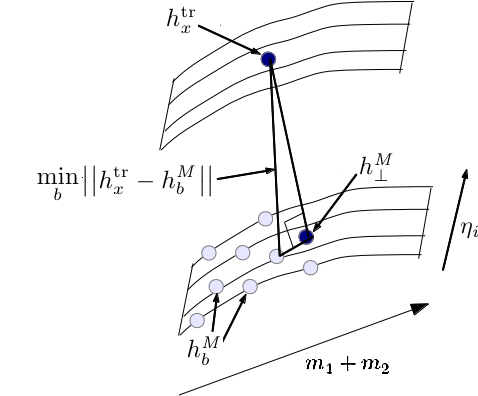
\includegraphics[width=\columnwidth]{figures/nrhybbank/Eff1v2.png}%\quad
\caption{We show the \textit{true} (upper) and the \textit{hybrid} (lower) 
waveform manifolds here, with the signal residing in the former, and a discrete
bank of templates placed along lines of constant mass-ratio in the latter. 
Both manifolds are embedded in the same space of all possible waveforms.
The true signal waveform is denoted as $h^{\tr}_x$, while the templates in the
bank are labelled $h^{\M}_b$. The hybrid waveform that matches the signal $H^{\tr}_x$
best is shown as $h^{\M}_\perp$. Also shown is the ``distance'' between
the signal and the hybrid template that has the highest overlap with it.
This figure is qualitatively similar to Fig.~3 of
Ref.~\cite{WaveformAccuracy2008}.}
\label{fig:EFFdiag1}
\end{figure}
% \begin{figure}
%  \centering
% 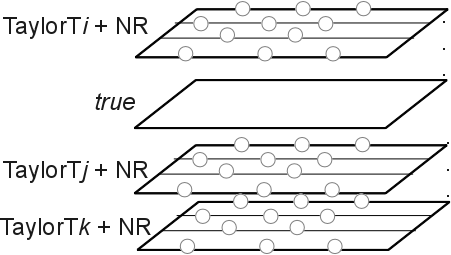
\includegraphics[width=0.8\columnwidth]{Eff2.png}%\quad
% \caption{We show the \textit{true} and the \textit{hybrid} waveform manifolds 
% relative to it. We assume that the hybrid waveform manifolds envelope 
% \textit{true} one, and so the shortest distance between a point on the true 
% manifold and any hybrid manifold would be lesser than the same between the two 
% mutually farthest hybrid manifolds; as for Eq.~(\ref{eq:hybridMMTn}).}
% \label{fig:EFFdiag2}
% \end{figure}
Fig.~\ref{fig:EFFdiag1} shows the signal $h^\tr_x$ in its manifold, and the
bank of templates $h^\M_b$ residing in the model waveform manifold, both being
embedded in the same space of all possible waveforms. The 
point $h^\M_\perp$ is the waveform which has the smallest mismatch
in the entire (continuous) model manifold with $h^\tr_x$, i.e.
$h^\M_\perp :\mathcal{M}(h^\tr_x,h^\M_\perp) = \underset{y}{\mn}\,\,\mathcal{M}(h^\tr_x,h^\M_y)$.
The fraction of the optimal SNR recovered at different points $x$ in the
binary mass space can be quantified by measuring the fitting factor $\FF$ of
the bank~\cite{FittingFactorApostolatos},
\begin{equation}\label{eq:ffmismatch}
 \FF(x) = 1 - \underset{b}{\mn}\,\,\mathcal{M}(h^\tr_x, h^\M_b).
\end{equation}
For two waveforms $h_1$ and $h_2$ close to each other in the
waveform manifold: $\leftn h_1\rightn \simeq\leftn h_2\rightn$, and mutually
aligned in phase and time such that the overlap between them is maximized, 
\begin{equation}
%  \begin{align}
  \leftn h_1 - h_2\rightn^2 \simeq 2\left( h_1 |h_1\right)\left(1 - \dfrac{\left( h_1 |h_2\right)}{\sqrt{\left( h_1 |h_1\right)}\sqrt{\left( h_1 |h_1\right)}}\right).
%  &= 2\leftn h_1\rightn^2 \Mis\left(h_1,h_2\right)
% \end{align}
\end{equation}
The mismatch can, hence, be written as 
(c.f. Eq.~(\ref{eq:mismatch}))
\begin{equation}
 \Mis\left(h_1,h_2\right) = \dfrac{1}{2\leftn h_1\rightn^2}\leftn h_1 - 
h_2\rightn^2.
\end{equation}
We note that this equation is an upper bound for Eq.~(25) of
Ref.~\cite{Cannon:2012gq}. 
From this relation, and treating the space embedding the true and model 
waveform manifolds as Euclidean at the scale of template separation, we
can separate out the effects of bank coarseness and template inaccuracies as
\begin{subequations}
\begin{align}
 \FF(x) &= 1 - \underset{b}{\mn}\dfrac{1}{2\leftn h^\tr_x\rightn^2}\leftn h^\tr_x - h^\M_b\rightn^2 ,\\
 &= 1 - \Gamma_\Hyb(x) - \Gamma_\bnk(x)\label{eq:FFGammas};
 %&= 1 - \underset{b}{\mn}\dfrac{1}{2\leftn h^\tr_x\rightn^2}\leftn h^\tr_x - h^\M_\perp\rightn^2 - \underset{b}{\mn}\dfrac{1}{2\leftn h^\tr_x\rightn^2}\leftn h^\M_\perp - h^\M_b\rightn^2
 \end{align}
\end{subequations}
where 
\begin{equation}
\Gamma_\Hyb(x) \equiv \dfrac{1}{2\leftn h^\tr_x\rightn^2}\leftn h^\tr_x - h^\M_\perp\rightn^2 = \mathcal{M}(h^\tr_x,h^\M_\perp) 
\end{equation}
is the SNR loss from model waveform errors out of the manifold of true signals;
and 
\begin{equation}\label{eq:GammaBank}
\Gamma_\bnk(x) \equiv \underset{b}{\mn}\dfrac{1}{2\leftn h^\tr_x\rightn^2}\leftn h^\M_\perp - h^\M_b\rightn^2 = \underset{b}{\mn}\,\,\mathcal{M}(h^\M_\perp,h^\M_b) 
\end{equation}
is the loss in SNR from the distant spacing of templates in the bank.
The decomposition in Eq.~(\ref{eq:FFGammas}) allows for the measurement of the 
two effects separately. 
% When we use the NR simulations as templates, $\Gamma_\Hyb \simeq 0$, but 
% hybridizing them with PN inspirals will introduce waveform errors. 
NR-PN hybrids have the inspiral portion of the waveform, from PN theory, 
joined to the available late-inspiral and merger portion from NR (as described
in Sec.~\ref{s2:NRpNhybridwaveforms}). Towards the late inspiral, the PN
waveforms accumulate phase errors, contaminating the
hybrids~\cite{MacDonald:2011ne,MacDonald:2012mp}. For each hybrid, we constrain
this effect using mismatches between hybrids constructed from the same NR 
simulation and different PN models, i.e.
\begin{equation}
 \Gamma_\Hyb(x) \leq \mathcal{M}(h^\tr_x,h^\Hyb_x) \lesssim \underset{(i,j)}{\mx}\,\,\mathcal{M}(h^{\M_i}_x,h^{\M_j}_x),
\end{equation}
where  $\M_i = $ TaylorT[1,2,3,4]+NR.
However, this is only possible for a few values of mass-ratio for which NR
simulations are available. We assume $\Gamma_\Hyb$ to be a slowly and smoothly 
varying quantity over the component-mass space at the scale of template grid
separation. At any arbitrary point $x$ in the mass space we approximate 
$\Gamma_\Hyb$ with its value for the ``closest'' template, i.e.
\begin{equation}\label{eq:GammaHybfinal}
 \Gamma_\Hyb(x) \leq \underset{(i,j)}{\mx}\,\,\mathcal{M}(h^{\M_i}_x,h^{\M_j}_x) \simeq \underset{(i,j)}{\mx}\,\,\mathcal{M}(h^{\M_i}_b,h^{\M_j}_b),
\end{equation}
where $h^\M_b$ is the hybrid template in the bank with the highest overlap with 
the signal at $x$. 
% Since NR waveforms have a limited number of 
% orbits, to obtain $\Gamma_\Hyb$ for hybrids with lower matching frequencies, 
% their NR portion is replaced with EOBNRv2 waveforms. As only the PN
% portion is changing in these comparisons, and the EOBNRv2 model was calibrated 
% against most of the NR simulations that we use here~\cite{BuonannoEOBv2Main}, 
% using EOBNRv2-PN hybrids gives the same measurements as using NR-PN hybrids for
% hybrid mismatches.

The other contribution to SNR loss comes from the discrete placement of 
templates in the mass space. In Fig.~\ref{fig:EFFdiag1}, this is shown in the
manifold of the template model. As NR waveforms (or hybrids) are available
for a few values of mass-ratio, we measure this in the manifold of EOBNRv2
waveforms. The EOBNRv2 model reproduces most of the NR simulations that
were consider here well~\cite{BuonannoEOBv2Main}, allowing for this 
approximation to hold. For the same reason, we expect $h^\EOB_x$ to be close to 
$h^\EOB_\perp$, with an injective mapping between the two. This allows us to 
approximate (c.f. Eq.~(\ref{eq:GammaBank}))
\begin{eqnarray}\label{eq:GammaBankEOB}
\label{eq:Gammabnkfinal}
 \Gamma_\bnk(x) &\simeq & \underset{b}{\mn}\,\,\mathcal{M}(h^\EOB_x,h^\EOB_b).
\end{eqnarray}

In Sec.~\ref{s1:NRonlybank}, we construct template banks that use purely-NR
templates, which have negligible waveform errors. The SNR recovery from such 
banks is characterized with
\begin{equation}\label{eq:NRFFGammas}
 \FF(x) = 1 - \Gamma_\bnk(x),
\end{equation}
where the SNR loss from bank coarseness is obtained using 
Eq.~(\ref{eq:Gammabnkfinal}). In 
Sec.~\ref{s1:NRpNhybridbank},~\ref{s1:futureNRpNhybridbank}, we construct 
template banks aimed at using NR-PN hybrid templates. Their SNR recovery is
characterized using Eq.~(\ref{eq:FFGammas}), where the additional contribution
from the hybrid waveform errors are obtained using Eq.~(\ref{eq:GammaHybfinal}).


% For the NR-PN hybrid template bank, as we do not know the \textit{true} 
% waveforms at arbitrary points in the signal parameter space (the component
% masses of the binary), we estimate the $\FF$ as follows. Let us
% parametrize the mass parameter space by $\eta$ and $M$, noting the bijective
% mapping
% $\eta =q/(1+q)^2$. 
% For any point in the mass space $(\eta,M)$, we re-write the $\FF$ as
% \begin{subequations}
% \begin{align}
%  \FF(\eta,M) &\equiv 1 - 
% \underset{\eta',M'}{\mn}\Mis\left(h^{\tr}(\eta,M),h^{\M}_g(\eta',M')\right) \\
%  %
%  \simeq & 1 - \dfrac{1}{2\leftn h\rightn^2}\,\, \underset{\eta',M'}{\mn} \leftn 
% h^{\tr}(\eta,M)-h^{\M}_g(\eta',M')\rightn^2 \label{eq:FFasnormsq} \\
%  \equiv & 1 - \dfrac{1}{2\leftn h\rightn^2}\,\E(\eta,M)
% \end{align}
% \end{subequations}
% where $\leftn h\rightn\equiv \leftn h^{\tr}(\eta,M)\rightn \simeq \leftn 
% h^{\M}_g(\eta',M')\rightn$, and $\E(\eta,M)\equiv \underset{\eta',M'}{\mn} \leftn 
% h^{\tr}(\eta,M)-h^{\M}_g(\eta',M')\rightn^2$. 
% %What we want to constrain, at each point $(\eta ,M)$ in the region of 
% %component mass space that our NR-PN-hybrid bank aims to cover is
% % \begin{multline}
% %  \underset{\eta_i,M_A}{\mn} \leftn h^{\tr}(\eta,M) - 
% % h^{\M}_g(\eta_i,M_A)\rightn^2 \notag\\
% %  = 2\rho\,(1-\FF_{\Hyb}(\eta,M)) \equiv \E(\eta,M),
% % \end{multline}
% %where $\rho$ in the expected matched-filter signal-to-noise-ratio (SNR) for the 
% %signal with source parameters $(\eta, M)$.
% As in Ref.~\cite{WaveformAccuracy2008,WaveformAccuracy2010}, we visualize the
% waveforms in their manifold in Fig.~\ref{fig:EFFdiag1}, where the top manifold
% is that of the \textit{true} waveforms, and the bottom is the model waveform 
% manifold; while the parallel lines are contours of constant mass-ratio with 
% total mass $M$ increasing from left to right (clockwise). The NR and the NR-PN
% hybrid bank grids are restricted to occupy these contours as NR simulations are 
% only available for a discrete set of mass-ratios, but can be rescaled to 
% different values of total mass. The quantity $\E$ is depicted in the figure as
% the ``distance'' between the \textit{true} signal and the \textit{closest}
% template in the bank of hybrid waveforms (squared). We drop a \red{[Word missing here?]} perpendicular 
% from the signal at $(\eta, M)$ in the \textit{true} manifold to the hybrid 
% waveform manifold at $(\eta_{\perp}'', M_{\perp}'')$, i.e.
% \begin{multline}
% (\eta_{\perp}'', M_{\perp}''):\,\leftn h^{\tr}(\eta,M) - h^{\M}(\eta_{\perp}'', M_{\perp}'')\rightn \notag\\
%  = \underset{\eta'',M''}{\mn} \leftn h^{\tr}(\eta,M) - h^{\M}(\eta'', 
% M'')\rightn.
% \end{multline}
% As waveforms are smooth functions of the masses, their manifolds are
% expected to be smooth and the mapping $T:(\eta,M)\rightarrow (\eta_{\perp}'', 
% M_{\perp}'')$ to be unique. Assuming both true and approximant waveform 
% manifolds are in a locally Euclidean space (over ``distances''
% at the scale of template separation) we can write $\E(\eta,M)$ as
% \begin{subequations}
% \begin{align}
%  \E(\eta,M) &= \underset{\eta'',M''}{\mn} \leftn h^{\tr}(\eta,M) - h^{\M}(\eta'', M'')\rightn^2 \notag\\
%  & + \underset{\eta',M'}{\mn} \leftn h^{\M}(\eta_{\perp}'', M_{\perp}'') - 
% h^{\M}_g(\eta', M')\rightn^2 \label{eq:MMaddQuad1}\\
%  &\equiv \Delta_1 + \Delta_2(\eta_{\perp}'', M_{\perp}''),
% \end{align}
% \end{subequations}
% where $\Delta_1 =\Delta_1(\eta,M) =\Delta_1\left(T^{-1}(\eta_{\perp}'', M_{\perp}'')\right)$ 
% and $\Delta_2(\eta_{\perp}'', M_{\perp}'')$ are 
% abbreviations for the first and second terms in Eq.~\ref{eq:MMaddQuad1}, 
% respectively. 
% 
% \red{[Harald:  The description here seems overly complicated.  Please reconsider whether all symbols introduced are really needed.  Also reconsider ordering to make the flow of ideas as smooth and uninterrupted as possible.  Specifically: (i) Is a symbol needed for the mapping $T$, or is it sufficient to define $\eta_\perp$ and $M_\perp$?  (ii) Do the symbols $\Delta_1$ and $\Delta_2$ need to have parameters attached to it inside parentheses?  If so, they are defined as functions, so define what the functions are.  I see $\Delta_1(...)$ used below {\em once} with different arguments.  If this is the only use, then it's easier to just spell out that one use, rather than to define a function (iii) if $\Delta_1$ needs to remain a function, be consistent with how you write it.  Either always with arguments or never.]}
% 
% The first of these
% \begin{equation}
%   \Delta_1(\eta,M)\leq \underset{M''}{\mn} \leftn h^{\tr}(\eta,M) - h^{\M}(\eta, M'')\rightn^2,
% \end{equation}
% where the RHS of this inequality is the quantity that we put a bound on to
% estimate the waveform errors for the NR-PN hybrids~\cite{MacDonald:2012mp}. 
% The hybridization of NR 
% simulations with different PN waveforms gives us different hybrids, all of which 
% reside in their own manifolds, as shown in Fig.~\ref{fig:EFFdiag2}. If we assume 
% that the \textit{true} manifold is enveloped between the different hybrid 
% manifolds, we can conservatively estimate
% \begin{equation}\label{eq:hybridMMTn}
%  \begin{split}
%   \Delta_1 & \leq \underset{M''}{\mn} \leftn h^{\tr}(\eta,M) - h^{\M}(\eta, M'')\rightn^2 \\
%   &\lesssim \underset{(i,j)}{\max}\, \underset{M''}{\mn} \leftn h^{\M_i}(\eta,M) - h^{\M_j}(\eta, M'')\rightn^2,
%  \end{split}
% \end{equation}
% \red{[Harald:  I don't think we ever did the minimization over $M''$ when computing PN-hybrid errors.]}
% \red{[Harald: The text presently discusses twice how PN-hybrid errors are determined, here and in Sec IIF.  It would be good to incorporate IIF into IIE.  However, spend an entire paragraph on how they are determined, they are too complicated to do in passing in a sentence or two.]}
% 
% 
% where $(\M_i,\M_j)$ are pairs of the same NR waveform hybridized with 
% different PN approximants. As we have NR simulations for restricted values of
% mass-ratio, estimation of $\Delta_1$ at arbitrary points in the component-mass
% space is difficult. Assuming $\Delta_1$ to be a slowly varying quantity over the 
% component-mass space at the scale of template grid separation, we approximate 
% $\Delta_1 (\eta_{\perp}'', M_{\perp}'')\simeq\Delta_1(\eta_{g_c},M_{g_c})$,
% where $(\eta_{g_c},M_{g_c})$ is the closest template grid point to 
% $(\eta_{\perp}'', M_{\perp}'')$, obtained by maximizing
% $\Olap(h^{\M}(\eta_{\perp}'', M_{\perp}''),h^{\M}(\eta_{g_c},M_{g_c}))$.
% Then, the fitting factor at a point $(\eta,M)$ in the true manifold, and at
% $(\eta_{\perp}'', M_{\perp}'')$ in the model waveform manifold becomes
% %\begin{equation}
% \begin{subequations}\label{eq:FFConstraint}
%  \begin{align}
% \FF(\eta,M) &\lesssim 1 - \underset{(i,j)}{\mx}\,\underset{M''}{\mn}\,\,  \mathcal{M}\left(h^{\M_i}(\eta_{g_c},M_{g_c}), h^{\M_j}(\eta_{g_c}, M'')\right) \label{eq:effdef1}\notag\\
%  &\,\, - \underset{\eta_i,M_A}{\mn}\mathcal{M}\left(h^{\M}(\eta_{\perp}'', M_{\perp}''),h^{\M}_g(\eta_i, M_A)\right)  \\
%  &\equiv 1 - \Gamma_{\Hyb}(\eta_{\perp}'', M_{\perp}'') - \Gamma_{\bnk}(\eta_{\perp}'', M_{\perp}'') \\
%  &= 1 - \Gamma_{\Hyb}\left(T(\eta, M)\right) - \Gamma_{\bnk}\left(T(\eta, M)\right) ,
%  \end{align}
% \end{subequations}
% %\end{equation}
% where $\Gamma_{\Hyb}$ and $\Gamma_{\bnk}$ are just the last two terms on the 
% RHS of Eq.~\ref{eq:effdef1}. To construct an effectual bank, therefore, we
% restrict $\Gamma_{\Hyb} + \Gamma_{\bnk}$ below $0.035\,(0.053)$ over the region
% the NR-only or the NR-PN hybrid bank is to cover, as discussed above.
% 
% 
% \red{[Harald: I didn't manage to follow the calculation in Sec IIE
%   within the time I spent on it.  Perhaps it would be clearer to
%   reorganize the argument to arrive quickly at
% \begin{equation}
% FF(\eta, M) \lesssim 1- \Gamma_{\rm Hyb} - \Gamma_{\rm bank},
% \end{equation}
% as a sum of terms orthogonal to the model manifold, and tangential to
% the model manifold.  After this equation has been obtained, consider
% each of the $\Gamma_{\rm bank/Hyb}$ separately with its own sequence
% of inequalities.]}
% 
% 
% 
% 
% % From Eq.~\ref{eq:FFasnormsq}
% % \begin{equation}
% %  \FF(\eta,M) = 1 - \dfrac{1}{2\leftn h\rightn^2}\,\, \underset{\eta',M'}{\mn}
% %\leftn h^{\tr}(\eta,M)-h^{\M}_g(\eta',M')\rightn^2,
% % \end{equation}
% % we need to find an upper bound on
% % $\leftn h^{\tr}(\eta,M)-h^{\M}_g(\eta',M')\rightn^2$, which we can constrain
% % over the component-mass region. Let 
% % \begin{equation}
% %  \epsilon_{\Hyb}(\eta,M) \equiv \leftn h^{\tr}(\eta,M)-h^{M}(\eta,M)\rightn^2,
% % \end{equation}
% % be the error norm for the Hybrid waveform ($\M = \Hyb$ here), and
% % \begin{equation}
% %  \epsilon_{\Hyb,\eta,\M}(\eta,M) \equiv \underset{\eta'',M''}{\mn}\leftn 
% % h^{\tr}(\eta,M)-h^{M}(\eta'',M'')\rightn^2
% % % \end{equation}
% % % is the waveform error norm margenalized over the subscripted mass parameters. 
% % % Also define $(\eta'_m,M'_m)$ as the parameter values on the model manifold
% % % \begin{multline}
% % %  (\eta'_m,M'_m): \leftn h^{\tr}(\eta,M) - h^{\M}(\eta'_m,M'_m)\rightn^2 = \\
% % %  \underset{\eta'',M''}{\mn}\leftn h^{\tr}(\eta,M) - 
% % h^{\M}(\eta'',M'')\rightn^2,
% % % \end{multline}
% % % at which the line drawn from the manifold of true waveforms starting at 
% % ($\eta,M$)
% % % is orthogonal to the $\M$ manifold (which is the manifold of Hybrid waveforms 
% % in
% % % our case). We can then write
% % % \begin{subequations}
% % %  \begin{align}
% % %   &\underset{\eta',M'}{\mn}\leftn h^{\tr}(\eta,M)-h^{\M}_g(\eta',M')\rightn^2 
% % \simeq \notag\\
% % %   &\quad\quad \leftn h^{\tr}(\eta,M) - h^{\M}(\eta'_m,M'_m)\rightn^2 +\notag\\
% % %   &\quad\quad\quad\quad\underset{\eta',M'}{\mn} \leftn h^{\M}(\eta'_m,M'_m) - 
% % h^{\M}_g(\eta',M')\rightn^2 \\
% % %   %
% % %   &= \epsilon_{\Hyb,\eta,\M}(\eta,M) + \epsilon_{\mm}(\eta'_m,M'_m) \\
% % %   %
% % %   &\leq \epsilon_{\Hyb,\M}(\eta,M) + 
% % \epsilon_{\mm}(\eta'_m,M'_m)\label{eq:mmtogridmm}
% % %  \end{align}
% % % \end{subequations}
% % % where $\epsilon_{\Hyb,\M}(\eta,M)$ is the hybrid waveform error minimized 
% % over 
% % only the total mass at the point ($\eta,M$) and $\epsilon_{\mm}(\eta'_m,M'_m)$ 
% % is the loss due to 
% % % discretization of the bank grid at the point ($\eta'_m,M'_m$). Now, if we 
% % term 
% % the
% % % maximum loss due to a discrete grid $\epsilon_g$ (and call it \textit{grid} 
% % maximal
% % % mismatch), i.e.
% % % \begin{align}
% % %  \epsilon_g &\equiv 
% % \underset{\eta'_m,M'_m}{\mx}\epsilon_{\mm}(\eta'_m,M'_m)\notag\\
% % %  &\equiv \underset{\eta'_m,M'_m}{\mx}\underset{\eta',M'}{\mn} \leftn 
% % h^{\M}(\eta'_m,M'_m) - h^{\M}_g(\eta',M')\rightn^2,
% % % \end{align}
% % % we have, from Eq.~\ref{eq:mmtogridmm},
% % % \begin{equation}
% % %  \underset{\eta',M'}{\mn}\leftn h^{\tr}(\eta,M)-h^{\M}_g(\eta',M')\rightn^2 
% % \leq  \epsilon_{\Hyb,\M}(\eta,M) + \epsilon_g.
% % % \end{equation}
% % % \textit{If we assume that $\epsilon_{\Hyb,\M}(\eta,M)$ is a slowly varying 
% % function of the 
% % % mass-parameters compared to the grid density}, 
% % % i.e. $\epsilon_{\Hyb,\M}(\eta,M)\simeq \epsilon_{\Hyb,\M}(\eta',M')$,
% % % where $(\eta',M')$ are the parameters values of the closest point on the grid 
% % to
% % % ($\eta,M$), we get
% % % \begin{subequations}
% % % \begin{align}\label{eq:Finmms}
% % %  \underset{\eta',M'}{\mn}\leftn h^{\tr}(\eta,M)-h^{\M}_g(\eta',M')\rightn^2 
% % \leq  \epsilon_{\Hyb,\M}(\eta',M') + \epsilon_g \\ \label{eq:FinFFs}
% % %  \Rightarrow \FF(\eta,M) \geq 1 - \dfrac{1}{2\leftn 
% % h\rightn^2}\,\,\left(\epsilon_{\Hyb,\M}(\eta',M') + \epsilon_g\right)
% % % \end{align}
% % % \end{subequations}
% % % If we construct a bank, with 
% % % \begin{equation}
% % % \boxed{ \dfrac{1}{2\leftn h\rightn^2}\,\,\left(\epsilon_{\Hyb,\M}(\eta',M') + 
% % \epsilon_g\right) \leq 0.035;\,\,\forall\,(\eta',M')\in\mathrm{bank}},
% % % \end{equation}
% % % it should restrict the detection rate loss to below $\sim 10\%$. In other 
% % words,
% % % the tolerances we have to construct the NR-PN hybrid bank is
% % % \begin{equation}
% % %  \boxed{\MM_{\Hyb,\M} + \MM_g \leq 0.035}
% % % \end{equation}
% % % where $\MM_{\Hyb,\M}\equiv \underset{\eta',M'}{\mx}\left(\dfrac{1}{2\leftn 
% % h\rightn^2}\epsilon_{\Hyb,\M}(\eta',M')\right)$ is the hybrid waveform 
% % mismatch, 
% % % minimized over total-mass for each point in the bank, and subsequently 
% % maximized
% % % over the entire bank; and $\MM_g\equiv\dfrac{1}{2\leftn 
% % h\rightn^2}\,\epsilon_g$
% % % is the discretization mismatch measured using the same model as signal and 
% % template.
% 
% %\red{\em Describe how we derive an error-bound on a PN-NR hybrid waveform.}
% 
% The largest source of error in hybrid gravitational waveforms is
% caused by the higher-order unknown terms in the PN component. These
% cause different PN approximants to diverge as the binary black holes approach
% merger. In order to ascertain what this error is, we compare many
% types of PN waveforms and find the maximum mismatch between hybrids
% which use different PN approximants, in this case, Taylor T1, T2, T3,
% and T4. We assume this to be close to the actual PN error, as discussed in 
% Sec.~\ref{s2:quantifyingerrors}.
% 
% More specifically, we take four hybrid waveforms $h_\text{Tn}$, where $n = [1,2,3,4]$, and find their mismatches as defined in Eq.~\ref{eq:mismatch}:
% \begin{equation}
% \mathcal{M}_\text{max}(\eta,M) = \underset{(i,j)}{\mx}\,\underset{M''}{\mn}\,\,  \mathcal{M}\left(h^{\mathrm{T}i}(\eta,M), h^{\mathrm{T}j}(\eta,M'')\right) 
% \end{equation}
% $\mathcal{M}_\text{max}$ is what we call the hybridization error.
% 
% Because NR waveforms have a limited number of orbits, to obtain results for hybrids with lower matching frequencies, we replace the NR part of the hybrids with EOBNRv2 waveforms as described in Sec.~\ref{s2:EOBwaveforms}. Since only the PN waveforms are changing in these hybrid comparisons, using EOB hybrids gives the same results as using NR hybrids.

%\subsection{post-Newtonian uncertainties in hybrid waveforms}\label{s2:pNuncertainties}
%
%\red{\em Describe how we derive an error-bound on a PN-NR hybrid waveform.}

The largest source of error in hybrid gravitational waveforms is
caused by the higher-order unknown terms in the PN component. These
cause different PN approximants to diverge as the binary black holes approach
merger. In order to ascertain what this error is, we compare many
types of PN waveforms and find the maximum mismatch between hybrids
which use different PN approximants, in this case, Taylor T1, T2, T3,
and T4. We assume this to be close to the actual PN error, as discussed in 
Sec.~\ref{s2:quantifyingerrors}.

More specifically, we take four hybrid waveforms $h_\text{Tn}$, where $n = [1,2,3,4]$, and find their mismatches as defined in Eq.~\ref{eq:mismatch}:
\begin{equation}
\mathcal{M}_\text{max}(\eta,M) = \underset{(i,j)}{\mx}\,\underset{M''}{\mn}\,\,  \mathcal{M}\left(h^{\mathrm{T}i}(\eta,M), h^{\mathrm{T}j}(\eta,M'')\right) 
\end{equation}
$\mathcal{M}_\text{max}$ is what we call the hybridization error.

Because NR waveforms have a limited number of orbits, to obtain results for hybrids with lower matching frequencies, we replace the NR part of the hybrids with EOBNRv2 waveforms as described in Sec.~\ref{s2:EOBwaveforms}. Since only the PN waveforms are changing in these hybrid comparisons, using EOB hybrids gives the same results as using NR hybrids.


%%%%%%%%%%%%%%%%%%%%%%%%%%%%%%%%%%%%%%%%%%%%%%%%%%%%%%%%%%%%%%%%

%\section{Results}\label{s1:results}

\section{Constructing a template bank for NR waveforms}\label{s1:NRonlybank}

\begin{figure}
\centering
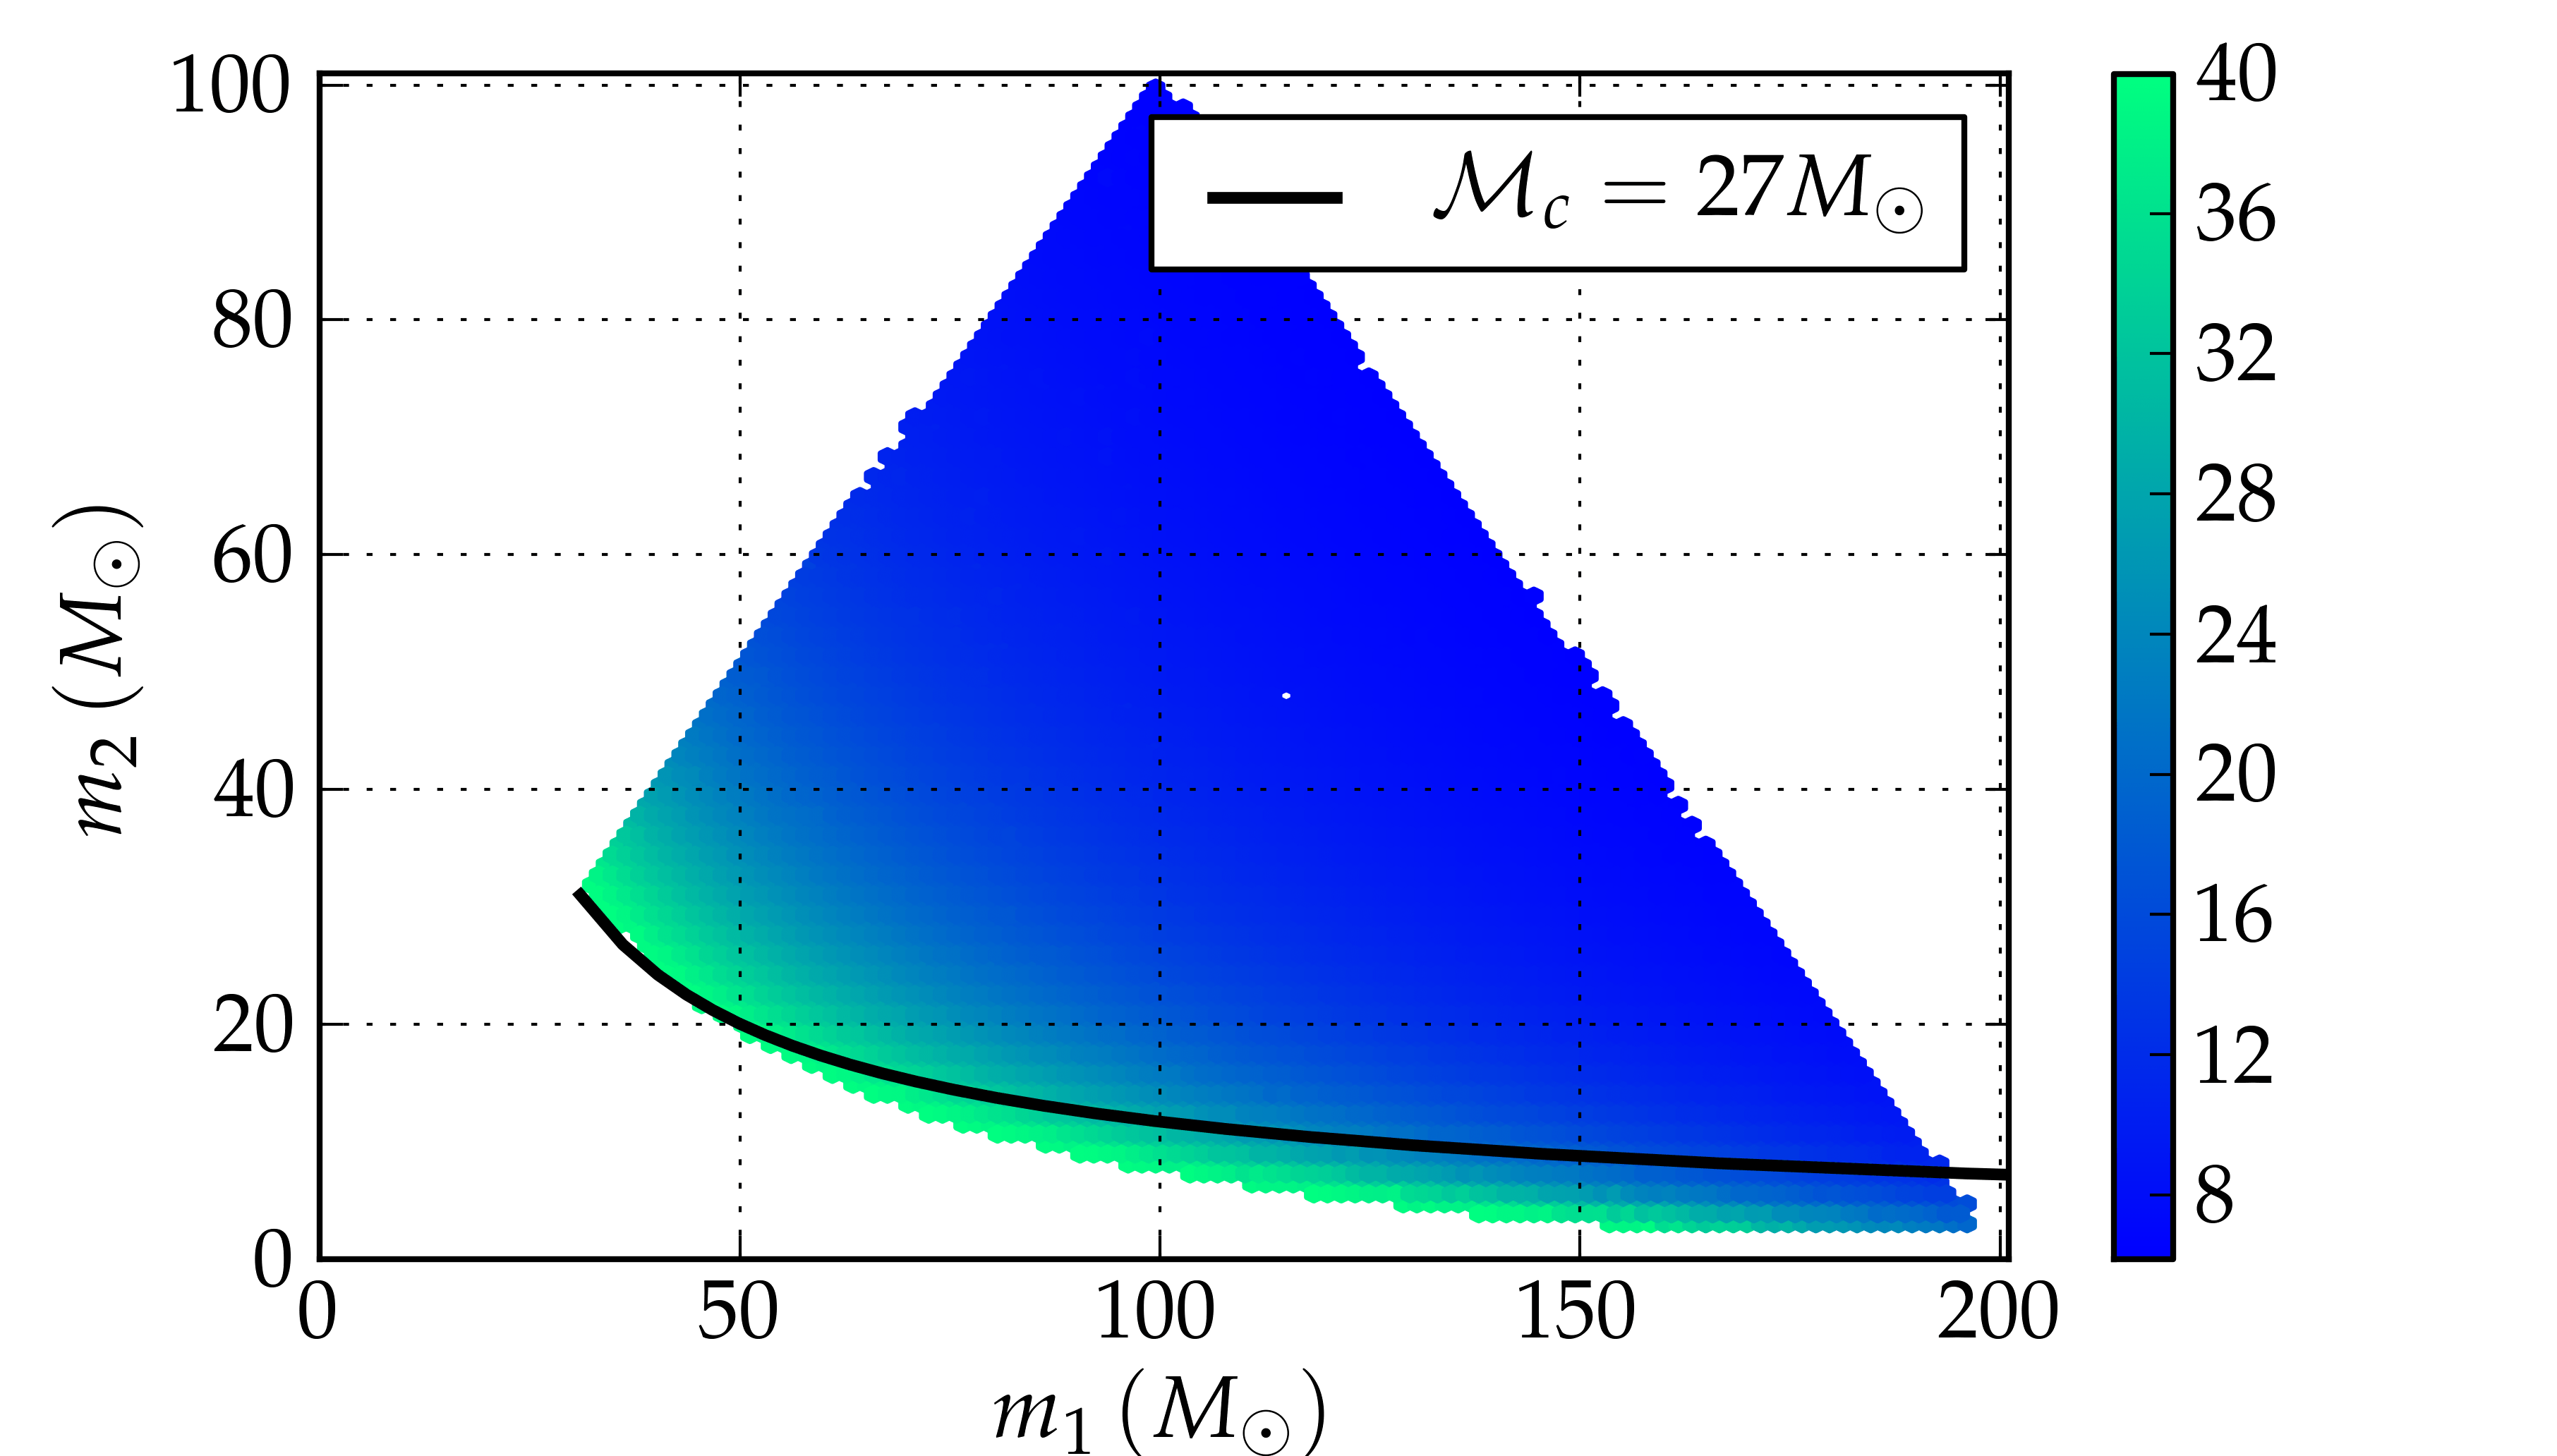
\includegraphics[width=1.1\columnwidth]{figures/nrhybbank/BBHm1m2_tlen_Ncyc40_0-99_Mchirp27_cropped-tiny.png}%\quad
%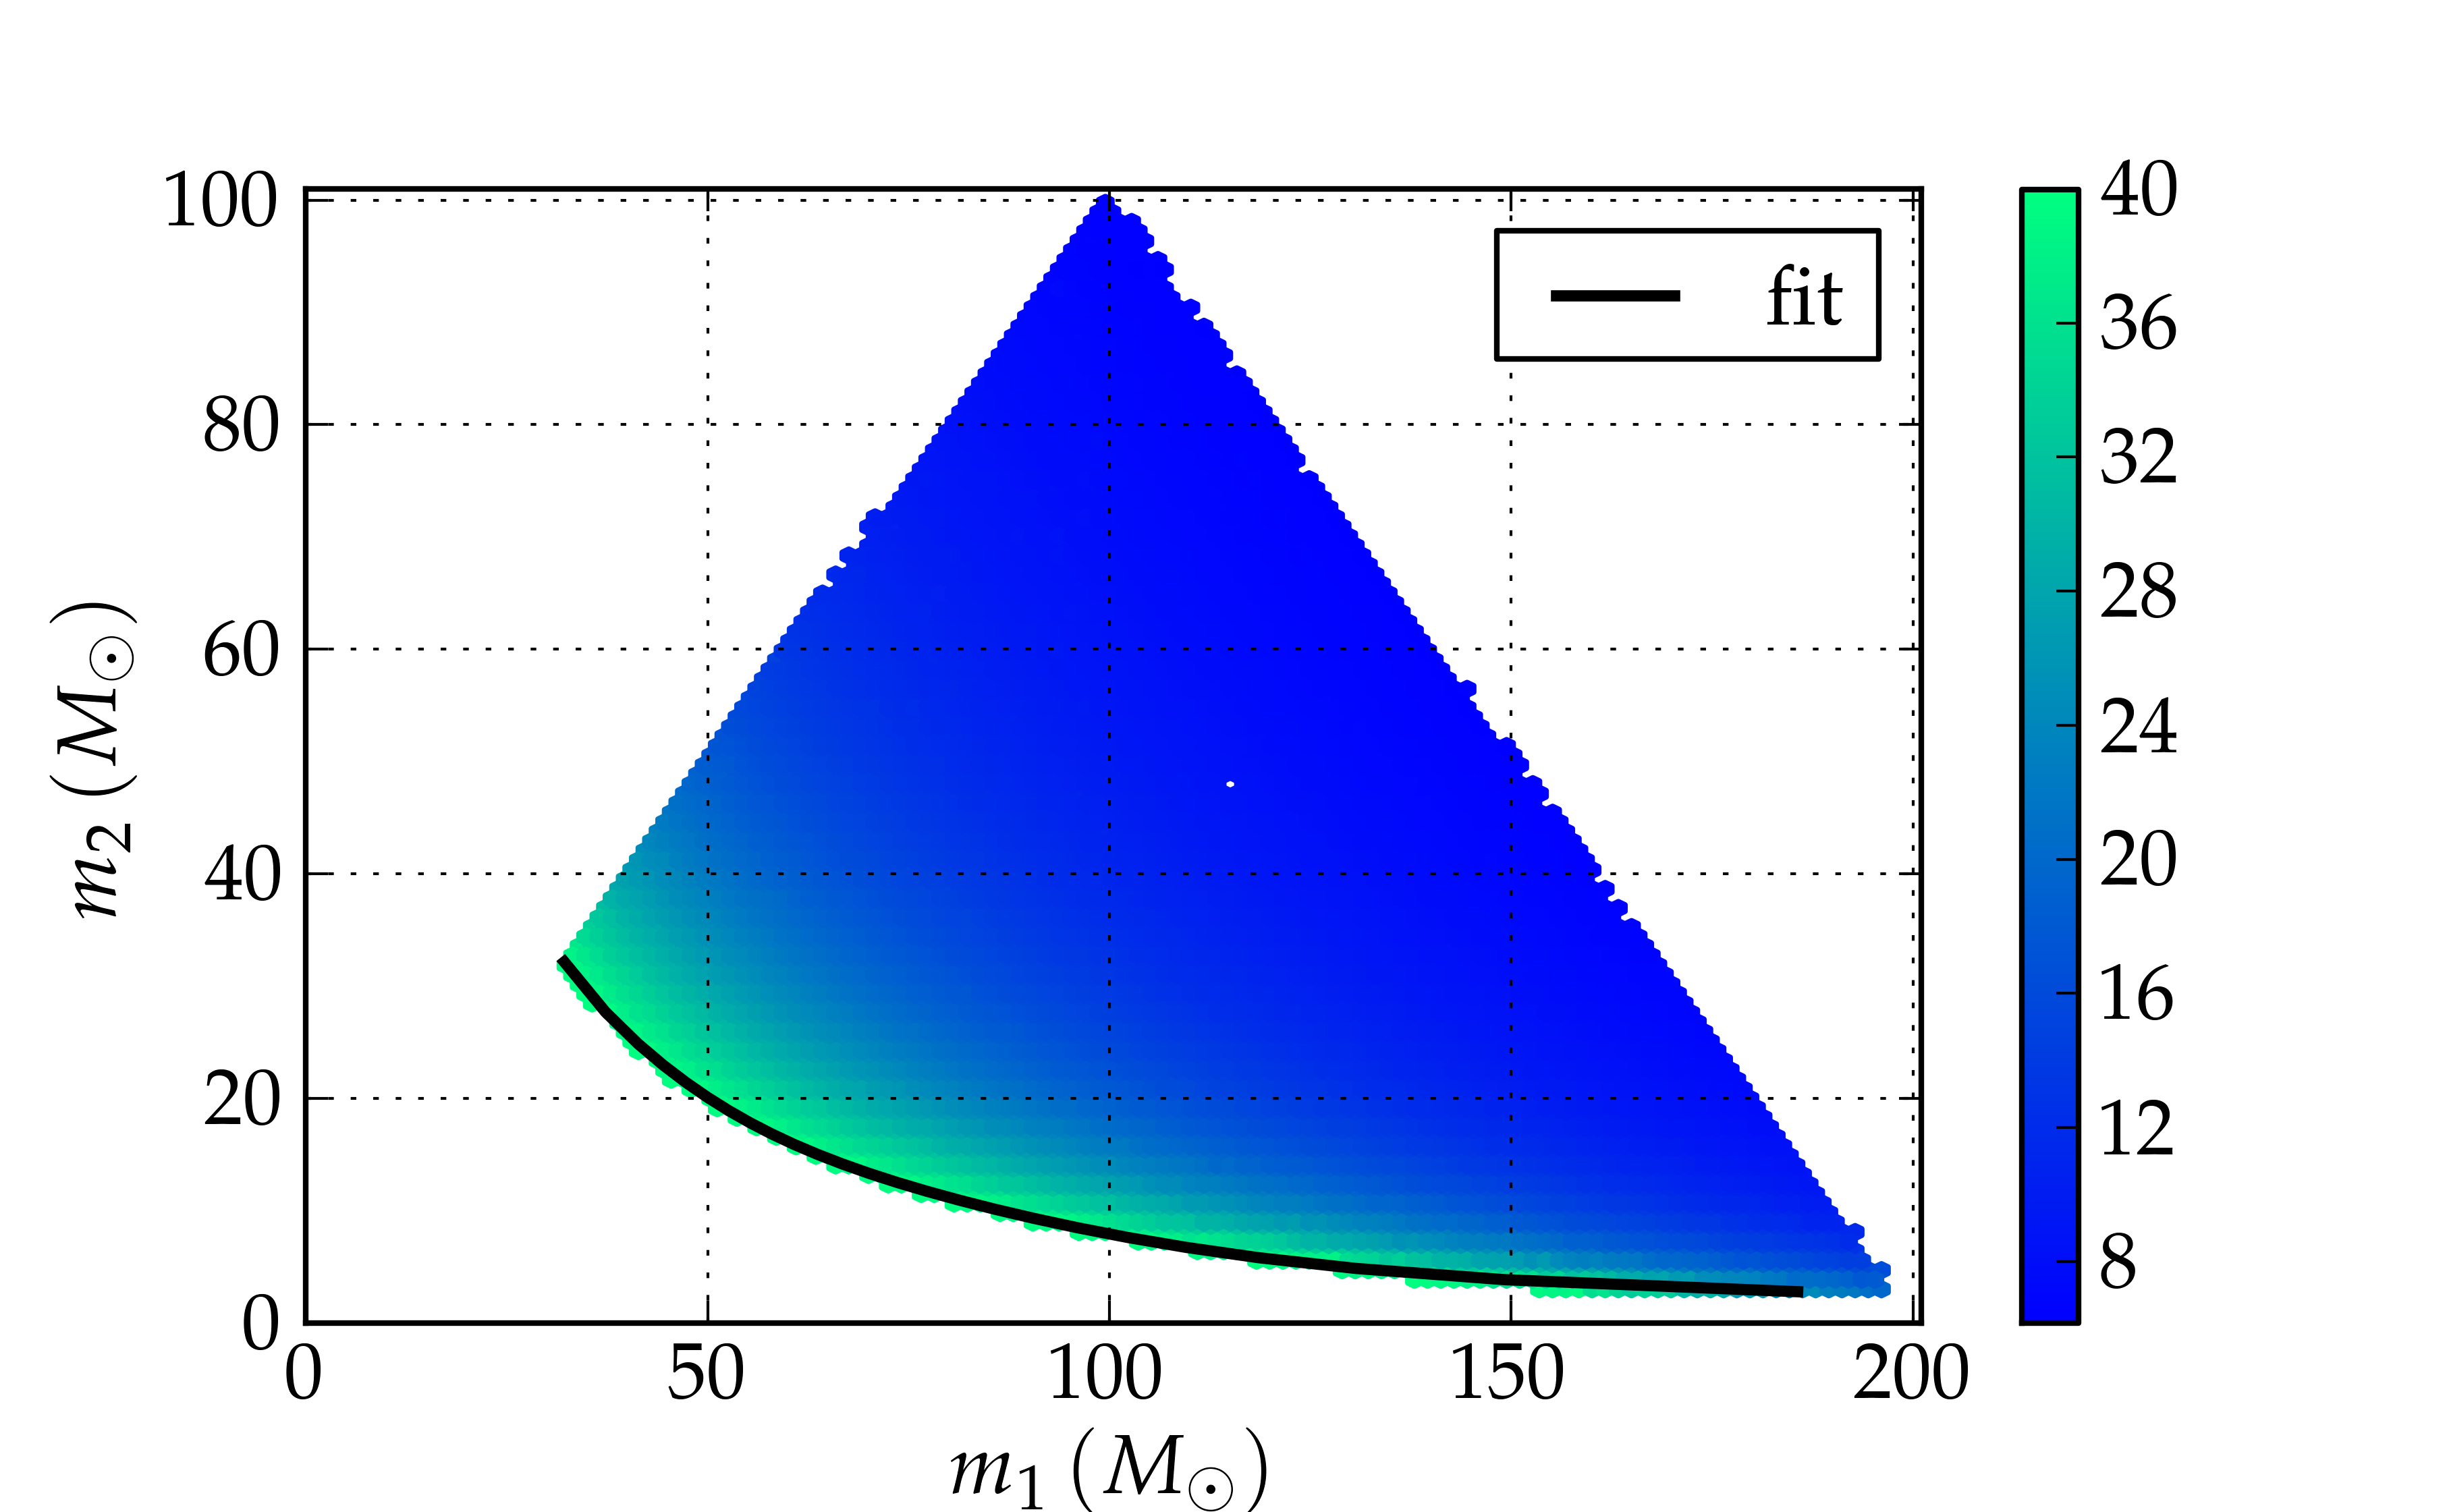
\includegraphics[width=\columnwidth]{BBHm1m2_0-99power_Ncyc40.png}
\caption{The color at each point gives the number 
of waveform cycles $\N_{\cyc}$, for that particular binary, which contain 
$99\%$ of the signal power in the aLIGO sensitivity band. The figure is 
trucated to exclude the region where $\N_{\cyc}>40$. The solid curve shows
the lower bounding edge of the region with $\mathcal{M}_c = 27M_\odot$.}
\label{fig:BBHregion}
\end{figure}

In this section we demonstrate the effectualness of a template bank viable
for using NR waveforms as templates. The gravitational-wave phase of the dominant 
waveform multipole 
extracted from runs at different resolutions was found to converge within 
$\sim 0.3\,\mathrm{rad}$ for $q=3,4,6$, and within $\sim 0.06\,\mathrm{rad}$
for $q=1,2$ at merger (see Fig.~(6) of Ref.~\cite{Buchman:2012dw}, and 
Fig.~(6,7) of Ref.~\cite{BuonannoEOBv2Main} for a compilation). Most of this 
phase disagreement accumulates over a relatively short duration of 
$\sim 50M  - 100M$ before merger, and is significantly lower over the preceding
inspiral and plunge. As the matched-filter SNR accumulates secularly over the
entire waveform, 
these numerical phase errors are negligible in terms of mismatches. We set
$\Gamma_\Hyb = 0$ while computing the fitting factors, so one is left with
considering $\Gamma_\bnk$ to determine the fidelity of the bank (c.f.
Eq.~(\ref{eq:FFGammas})).
% \red{[Harald: These figures compare EOB with NR.  
% How does this imply a statement about the accuracy of the NR waveforms?]}.
% \textcolor{blue}{This was left out at this place by error. The original
% context was the justification of using EOBNRv2 waveforms as
% proxies for NR simulations. I have removed it here.}

With NR simulations as templates, the region that the bank can cover is 
restricted to binaries that have approximately the same number of waveform 
cycles within the sensitive frequency band of the detectors as the simulations
themselves. We take their fiducial length to be $\sim 40$ GW
cycles~\cite{40GWcycles}. For BBHs with 
$3M_{\odot}\leq m_1,m_2\leq 200M_{\odot}$ and $m_1+m_2\leq 200M_{\odot}$ 
we map out the region with $99\%$ of the signal power within $40$ cycles as the
target region of the purely-NR bank. For samples taken over the mass space, we
determine the frequency interval $[f_1,f_2]$ for which
\begin{equation}\label{eq:99percentpower}
 \int_{f_1}^{f_2}\D f \dfrac{|\tilde{h}(f)|^2}{S_n(|f|)} = 
0.99\times\int_{f_\mathrm{min}}^{f_\mathrm{Ny}}\D f \dfrac{|\tilde{h}(f)|^2}{S_n(|f|)}.
\end{equation}
This is done by finding the peak of the integrand in 
Eq.~(\ref{eq:99percentpower}) and integrating symmetrically outwards from 
there, in time, till the interval $[f_1,f_2]$ is found. The number 
of waveform cycles in this interval is
\begin{equation}
 \N_{\cyc} = \dfrac{\Phi( t(f_2) ) - \Phi( t(f_1) )}{2\pi},
\end{equation}
where $\Phi(t)$ is the instantaneous phase of the waveform, 
${h_+(t)\,-\,\ii h_{\times}(t)\,=\,A(t)\,e^{-\ii \Phi(t)}}$, un-wrapped to be a
monotonic function of time. 
We find that for a significant portion of the mass-region, the signal power 
is contained within $40$ waveform cycles. This is shown in 
Fig.~\ref{fig:BBHregion}, where the color at each point gives $\N_{\cyc}$ for
that system, and the region with $\N_{\cyc}> 40$ is excluded. Conservatively, 
this region is bounded by $\mathcal{M}_c = 27M_\odot$, as shown by the solid 
curve in the figure.
% A fit for the total mass $M$ at the lower boundary of this region is given by
% \begin{equation}\label{eq:MtotalFit40Cycles}
% \begin{split}
%  M = \eta^{-3/5}&(12.02 + 217.76\eta - 1469.6\eta^2 + 5169.4\eta^3\\  
%  &-7011.5\eta^4),
%  \end{split}
% \end{equation}
% where $\eta = m_1m_2/M^2 = q/(1+q)^2$ is the symmetric mass-ratio.
% \red{[Harald: Eq (37) is very complicated.  It would be good to
%   give a simpler ``rule-of-thumb''.  By playing around, I found that
%   for the mass-ratios we are interested in, ${\cal M}_c=\mbox{const}$
%   works reasonably well.  I suggest to find the constant, point out that ${\cal M}_c\gtrsim XX$ is an approximation for $q<YY$, and also plot it in Fig. 3.]}


We place a bank over this region, using a stochastic method similar 
to Ref.~\cite{Harry:2009ea,Ajith:2012mn,Manca:2009xw}. 
The algorithm begins by taking an empty bank,
corresponding to step $0$. At step $i$, a proposal point $(q,M)$ is picked
by first choosing a value for $q$ from the restricted set
$\mathcal{S}_q=\{1,2,3,4,6,8\}$. The total mass $M$ is subsequently sampled
from the restricted interval corresponding to the pre-drawn $q$. The proposal 
is accepted if the waveform at this point has overlaps $\mathcal{O}< 0.97$ 
with all the templates in the bank from step $i-1$. This gives 
the bank at step $i$. The process is repeated till the fraction of 
proposals being accepted falls below $\sim 10^{-4}$, and $\gtrsim 99\%$
of the parameter space is covered effectually.
% \red{[Harald: I would have expected that by the time such a small acceptance fraction is reached, the bank is complete.  Is there a simple explanation why not?]}
% \textcolor{blue}{The acceptance rate decreases extremely rapidly as the bank
% converges to $> 99\%$ coverage fraction. This was shown in
% http://arxiv.org/abs/0908.2090 (Table II and Fig. 9). Table II
% shows that an acceptance ratio of $1$ in $10^4$ is achieved close to a 
% coverage fraction of $99.9\%$, while sampling in $\tau_0 - \tau_3$ coordinates.
% We can expect it to be lower for us as we sampled in $\mathcal{M}_c - \eta$ 
% coordinates.}
To complete the coverage, $100,000$ points are sampled over the region of mass
space depicted in Fig.~\ref{fig:BBHregion}, and $\FF$ of the bank
is computed at each point. With the islands of undercoverage isolated, the
points sampled in these regions are added to the bank, pushing their 
mass-ratios to the two neighboring mass-ratios in $\mathcal{S}_q$ 
along lines of constant chirp mass. 
This helps accelerate the convergence of the bank, albeit at the cost of 
over-populating it, as the algorithm for computing the $\FF$ for the 
sampled points is parallelizable.
\begin{figure}
\centering
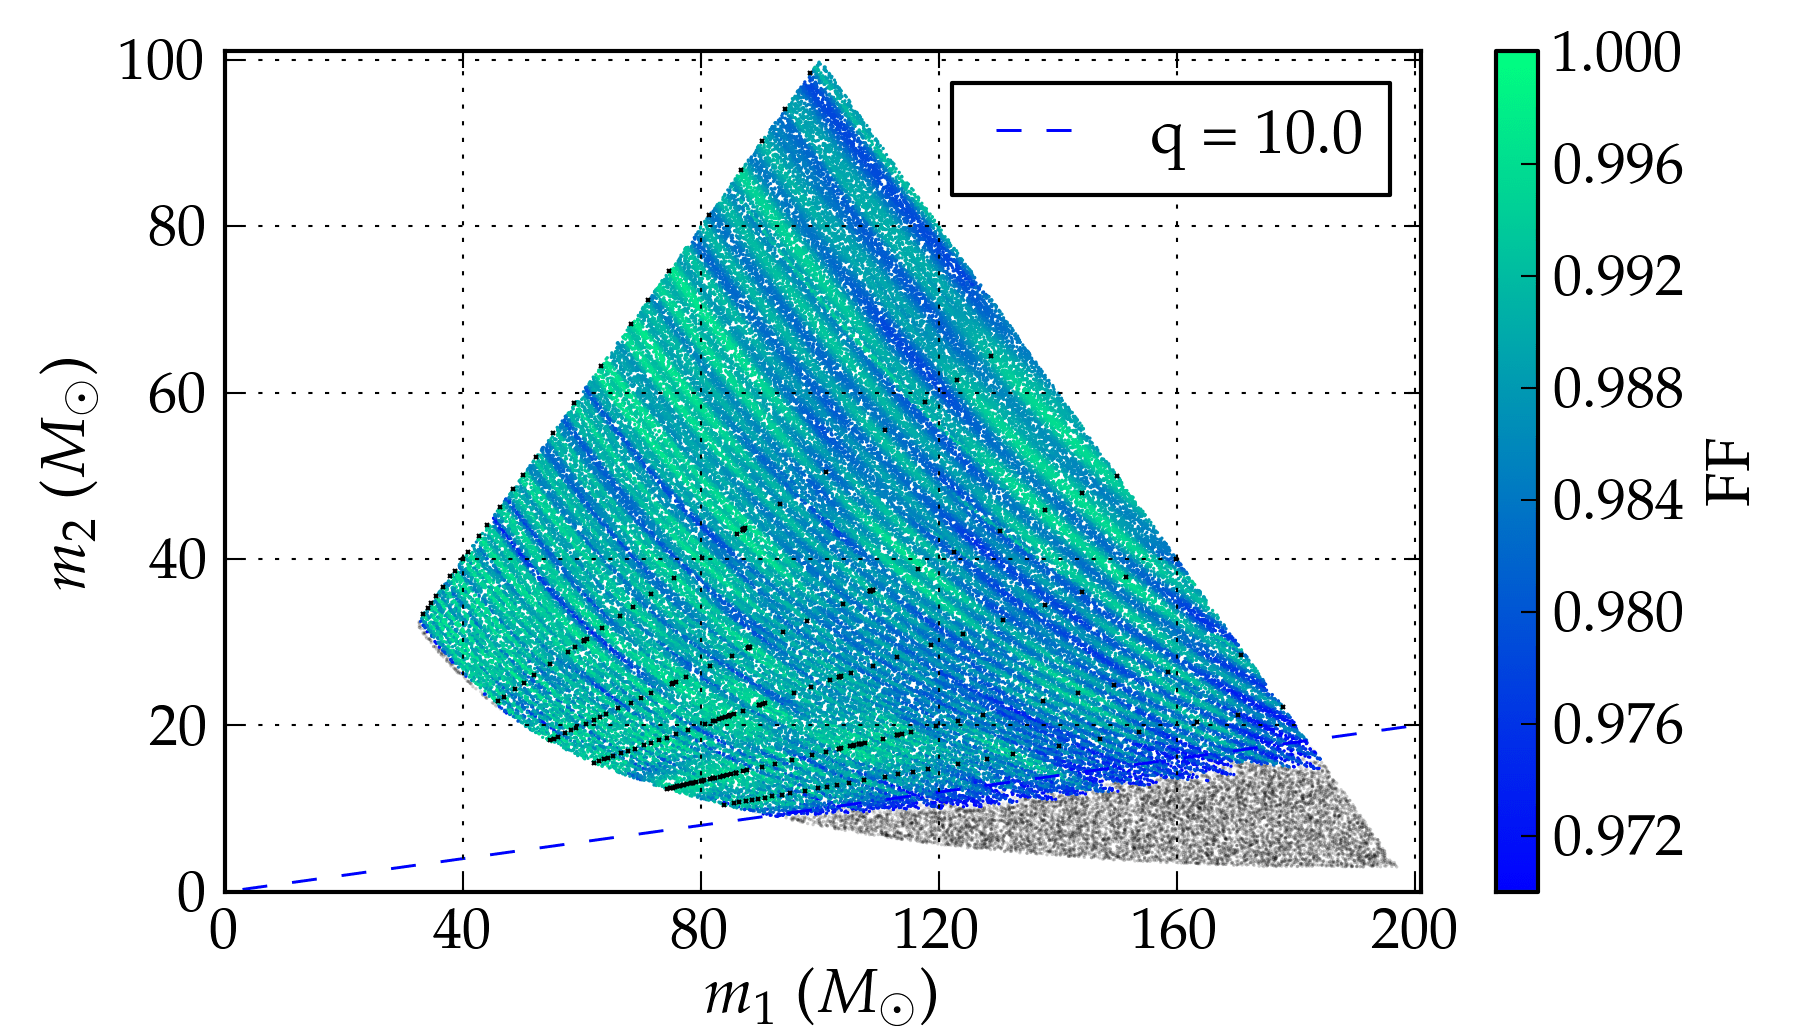
\includegraphics[width=\columnwidth]{figures/nrhybbank/bank002_01_01_mtot200_match_cropped-tiny.png}
%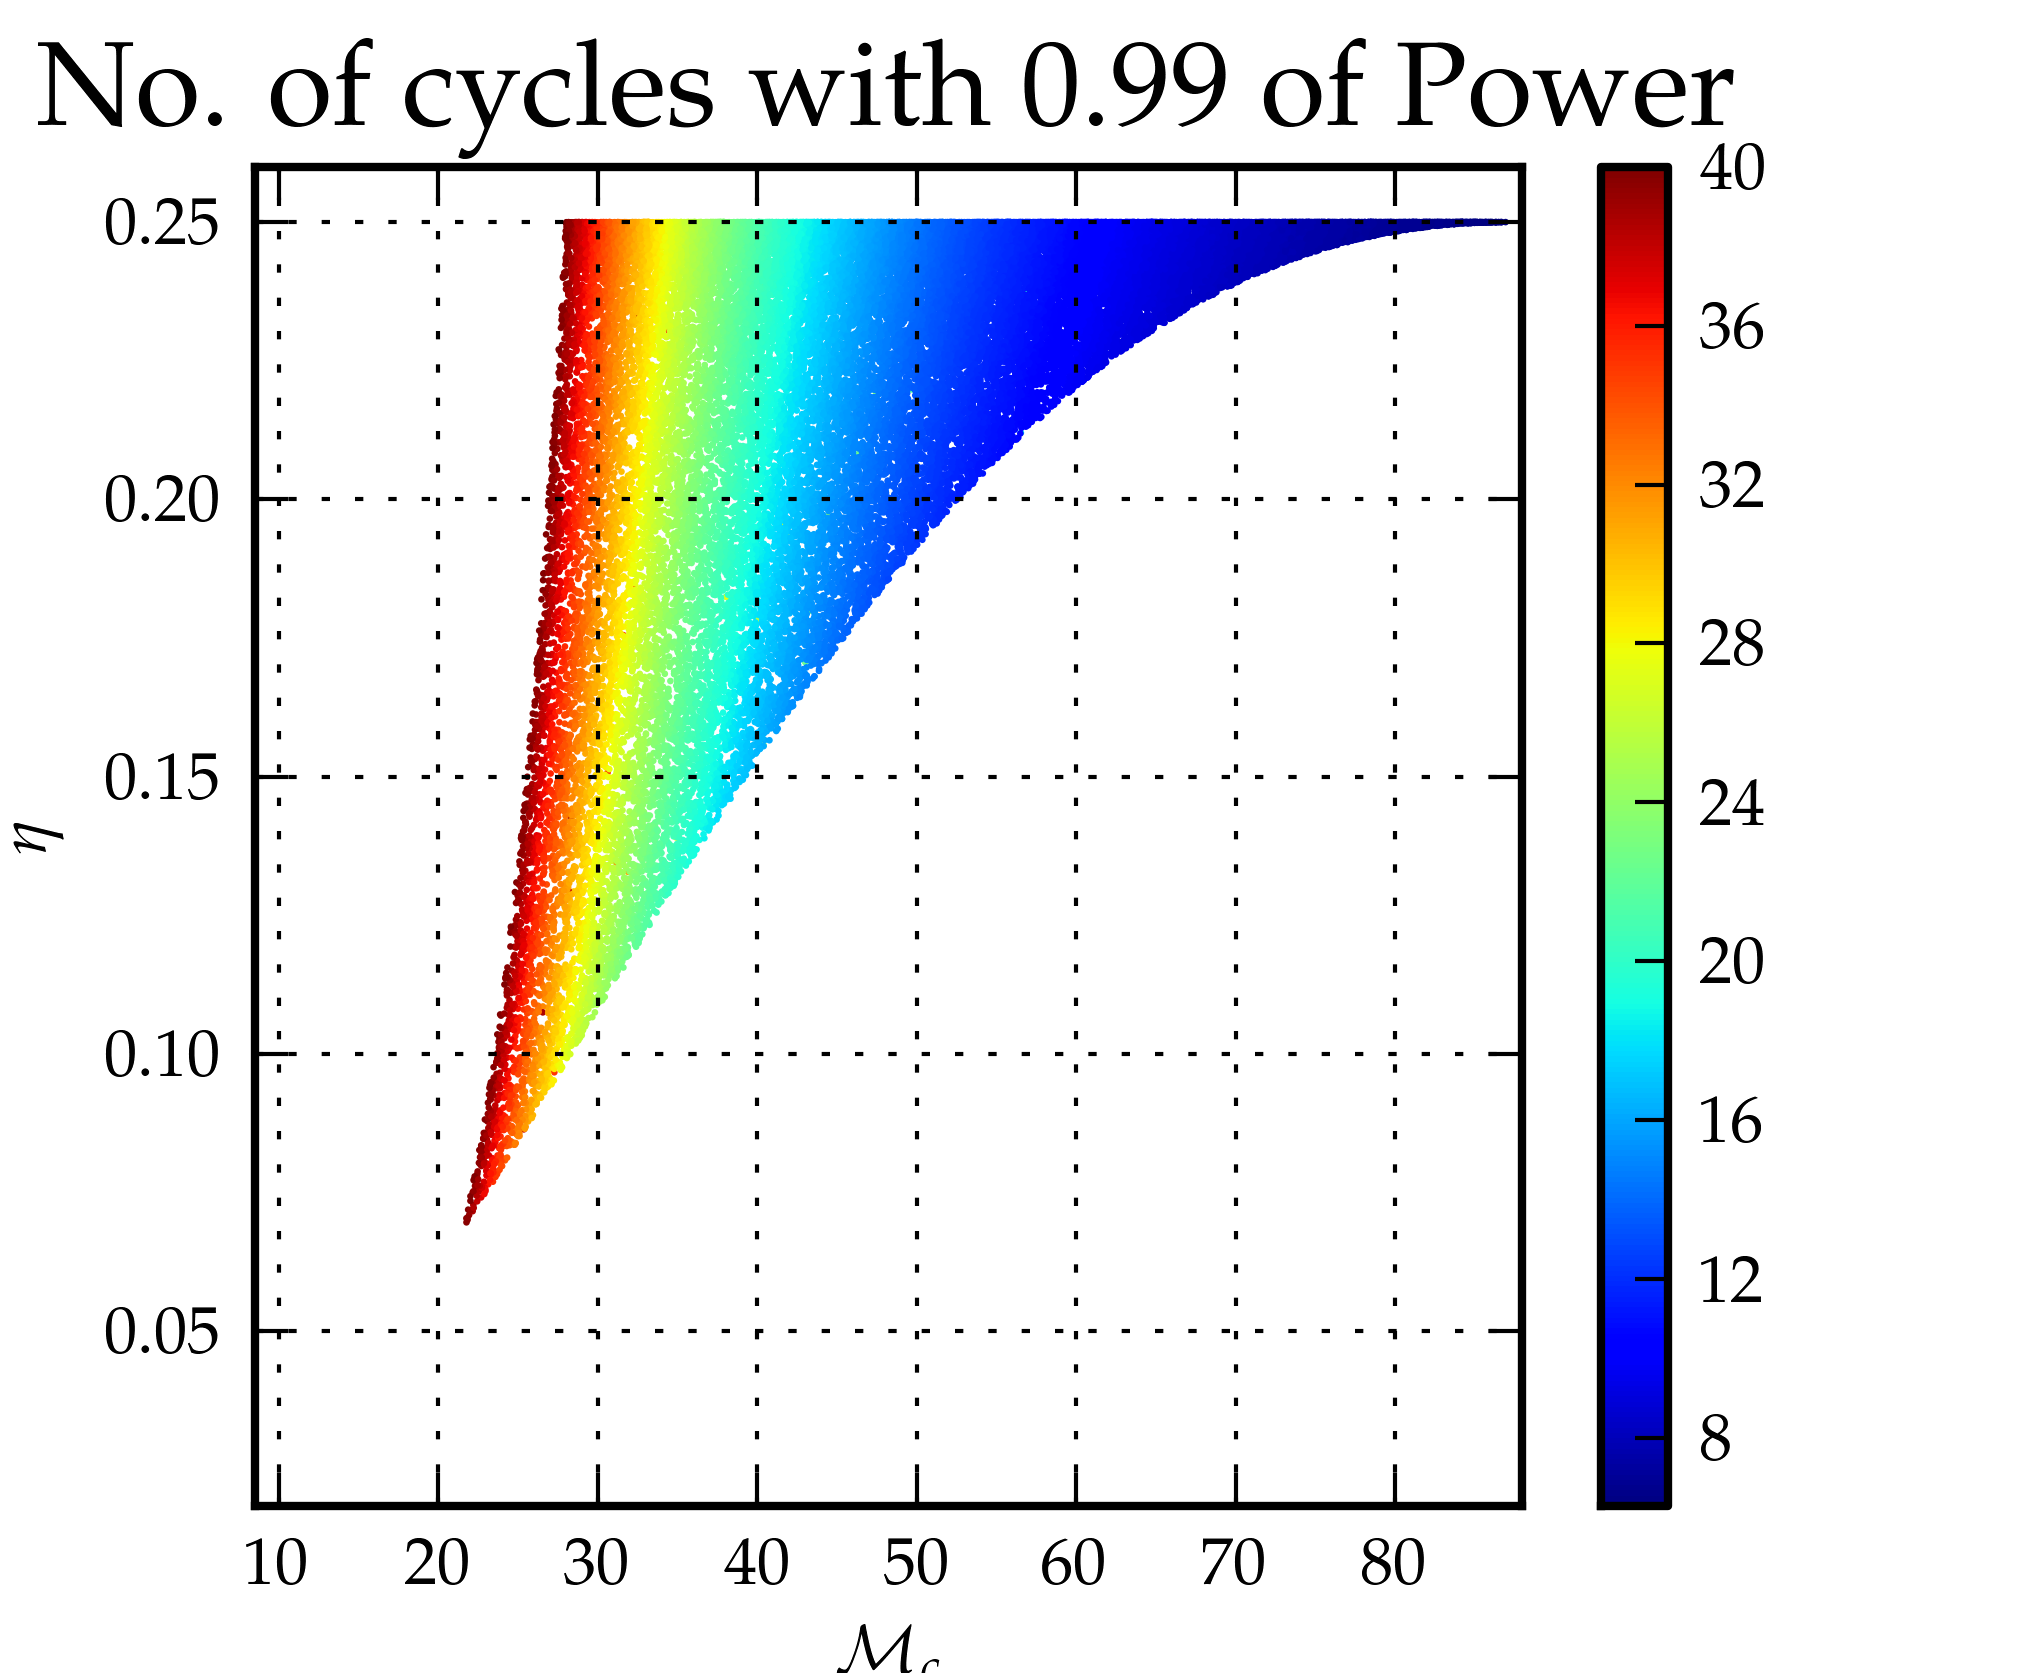
\includegraphics[width=\columnwidth]{BBHmcet_0-99power_Ncyc40.png}
\caption{The color at each point in the figure gives the
value of $\FF\simeq 1-\Gamma_{\bnk}$ of the bank for that binary, for
the NR bank restricted to $\mathcal{S}_q=\{1,2,3,4,6,8\}$. This is the
same as the fraction of the optimal SNR, for the binary, that the
template bank recovers. The black dots show
the location of the templates in the bank. We note that they all lie
along straight lines of constant $q$ passing through the origin. The region 
shaded light-grey (towards the bottom of the figure) is where the $\FF$ 
drops sharply below $97\%$.}
\label{fig:bank001_01_match}
\end{figure}
\begin{figure}
\centering
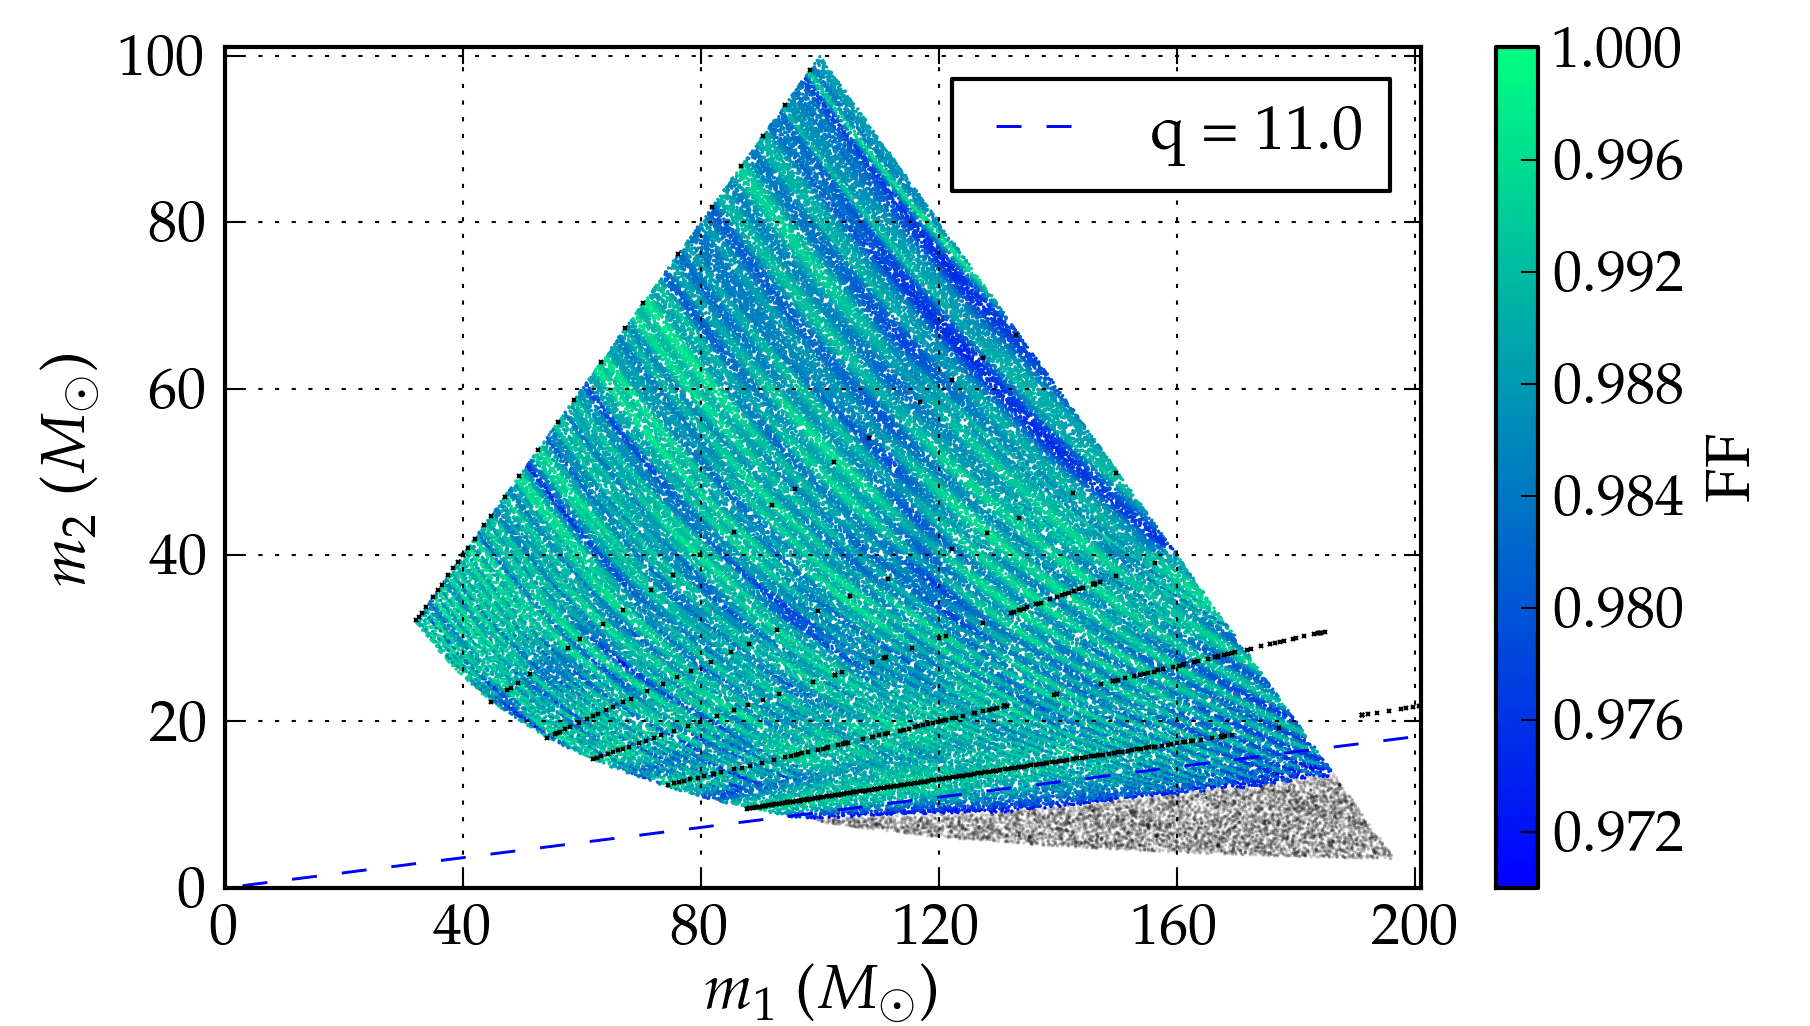
\includegraphics[width=\columnwidth]{figures/nrhybbank/bank006_01_mtot200_match_cropped-tiny.png}
%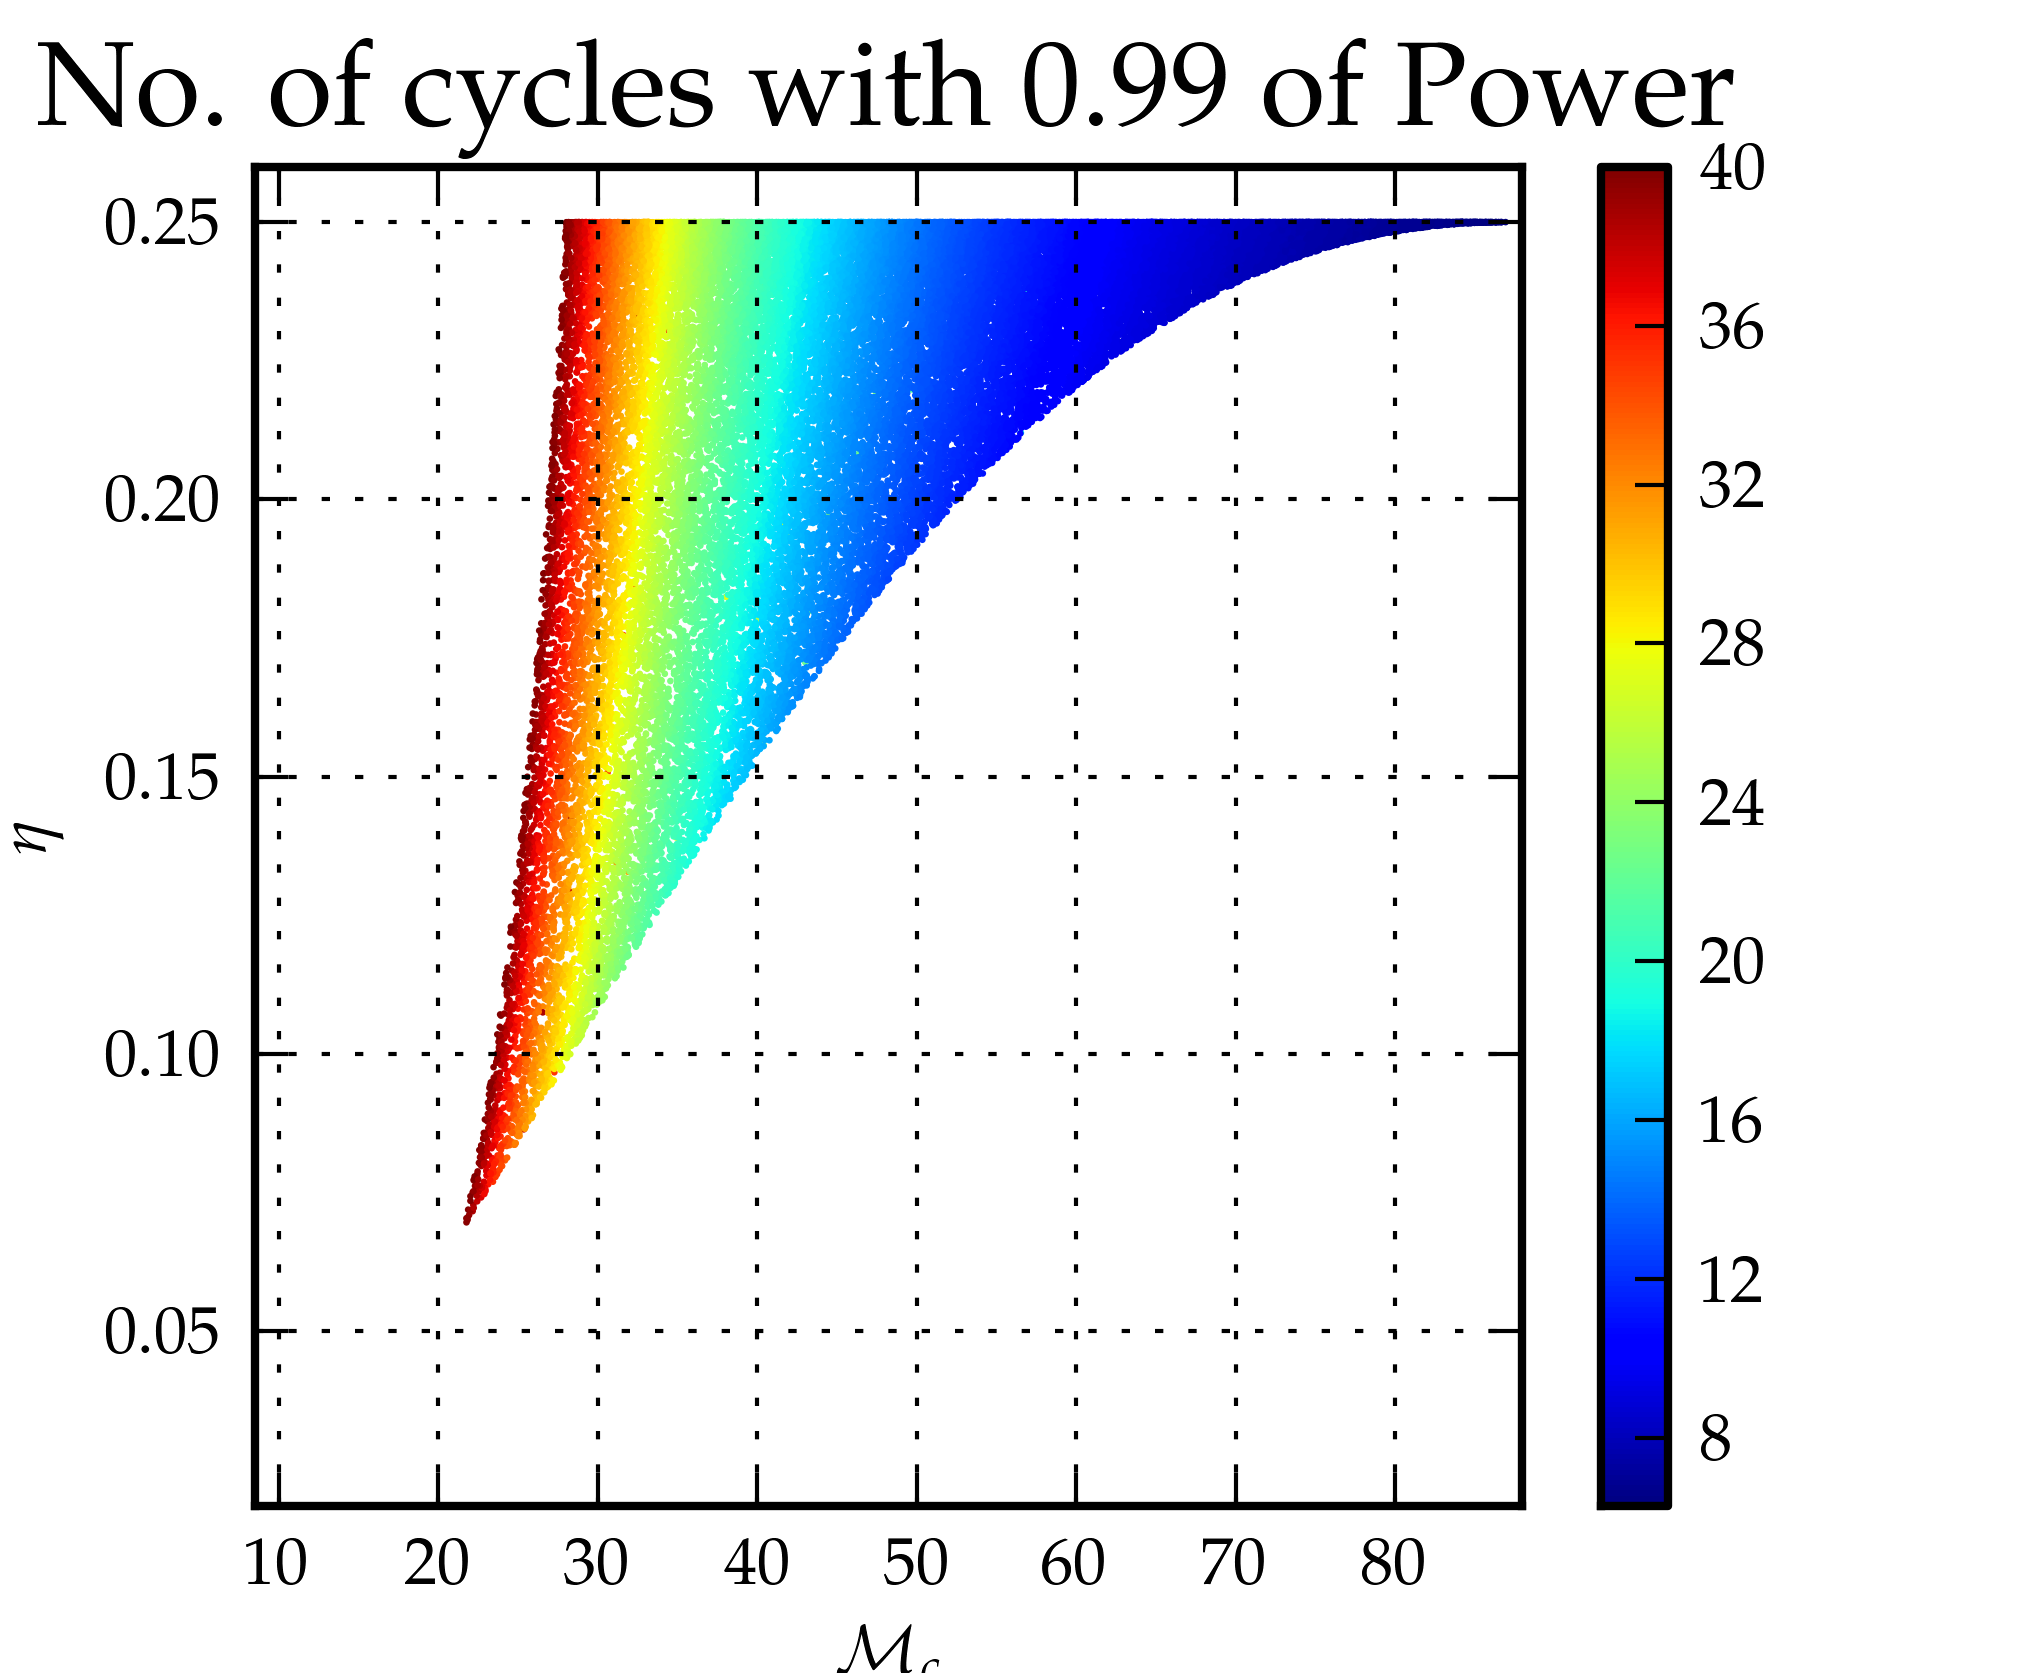
\includegraphics[width=\columnwidth]{BBHmcet_0-99power_Ncyc40.png}
\caption{This figure is similar to Fig.~\ref{fig:bank001_01_match}.
The color at each point gives the value of 
$\FF\simeq 1-\Gamma_{\bnk}$ of the bank for that binary, for
the NR bank restricted to $\mathcal{S}_q=\{1,2,3,4,6,9.2\}$.
The black dots show the location of the templates in the bank. 
The region shaded light-grey (towards the bottom of the figure) is 
where the $\FF$ drops below $97\%$. We note that with an additional
NR waveform for mass ratio $q=9.2$, the coverage of the bank is 
extended to include binaries with $10\leq q\leq 11$.}
\label{fig:bank006_01_match}
\end{figure}
% We test the bank so constructed by measuring the loss in the SNR that the 
% bank incurs for arbitrary incoming GW signals. As the waveform 
% mismatches due to the numerical errors are negligibly small, the primary cause
% for the loss in SNR would be the discreteness of the template bank grid. This
% effect can be measured by simulating BBH waveforms for various systems sampled
% over the region of the mass-parameter space that the bank intends to cover, and
% computing the fraction of optimal SNR that is recovered when these signals are
% filtered with our bank. 
% We need the signals and templates to be in the same
% manifold, to measure the effect of the discreteness of the bank alone.
% The recently proposed EOBNRv2 approximant~\cite{BuonannoEOBv2Main} was 
% calibrated to the numerical simulations for $q=\{1,2,3,4,6\}$, and thus 
% provides an excellent ground for that, i.e. superscript M~=~EOBNRv2 in
% $\Gamma_{\bnk}$ (Eq.~\ref{eq:FFConstraint}).

We asses the effectualness of the bank, as discussed in 
Sec.~\ref{s1:quantifyingerrors}, using Eq.~(\ref{eq:NRFFGammas}).
We draw a population of $100,000$ BBH signals, uniformly from the binary 
mass space, and filter them through the bank. Fig.~\ref{fig:bank001_01_match}
shows the $\FF$, or the fraction of the optimal SNR recovered by the bank. 
The region shown is restricted to binaries with $N_{\cyc}\leq 40$.
The black dots in the figure show the position of templates in the bank. 
The bank recovers $\geq 97\%$ of the optimal SNR over the entire region 
of interest for $q\leq 10$. We 
propose an additional simulation for $q=9.2$, to increase the coverage to
higher mass-ratios. Substituting this for $q=8$ in the set of allowed 
mass-ratios $\mathcal{S}_q$, we place another bank as before, with
$\mathcal{S}_q=\{1,2,3,4,6,9.2\}$. The SNR loss from this bank is shown in
Fig.~\ref{fig:bank006_01_match}. This bank recovers $\geq 97\%$ of the SNR for
systems with $q\leq 11$ and $\N_{\cyc}\leq 40$. The choice of the additional
simulation at $q=9.2$ was made by choosing a value \textit{close-to} the 
highest possible value of $q$ that does not lead to under-coverage in the 
region between $q=6$ and that value. The \textit{exact} highest allowed 
value was not chosen to reduce the sensitivity of the coverage of the bank
to fluctuations in detector sensitivity.

We conclude that with only six NR waveforms for non-spinning BBHs, that are
$\sim 20$ orbits (or $40$ GW cycles) in length, a template bank can be
constructed that is effectual for detecting binaries with chirp mass above
$27M_\odot$ and $1\leq q\leq 10$. With an additional 
simulation for $q=9.2$, this bank can 
be extended to higher mass-ratios, i.e. to $1\leq q\leq 11$.


\section{Constructing a template bank for NR-PN hybrids}\label{s1:NRpNhybridbank}

%\textcolor{red}{Why do we need a bank of hybrids?}\newline
The template bank contructed in Sec.~\ref{s1:NRonlybank} is effectual for 
GW detection searches focussed at relatively massive binaries with 
$\mathcal{M}_c \gtrsim 27M_\odot$. As the NR waveforms are restricted to a
small number of orbits, it is useful to consider NR-PN hybrids to bring the
lower mass limit down on the template bank. PN waveforms can be generated
for an arbitrarily large number of inspiral orbits, reasonably accurately and
relatively cheaply. Thus, a hybrid waveform comprised of a long PN early-inspiral 
and an NR late-inspiral, merger, and ringdown could also be arbitrarily long. 
There are, however, uncertainties in the PN waveforms, due to
the unknown higher-order terms. During the late-inspiral and merger phase,
these terms become more important and the PN description becomes
less accurate. In addition, when more of the late-inspiral is
in the detector's sensitivity frequency range, hybrid waveform mismatches 
due to the PN errors become increasingly large, and reduce the
recovered SNR. Thus, when
hybridizing PN and NR waveforms, there must be enough NR orbits that the PN
error is sufficiently low for the considered detector noise-curve. In 
this section, we construct an NR + PN hybrid template bank, for currently
available NR waveforms, and determine the lowest value of binary masses to 
which it covers.


%\subsubsection{Including hybrid PN error}\label{s2:HybridPNerror}
\begin{figure}
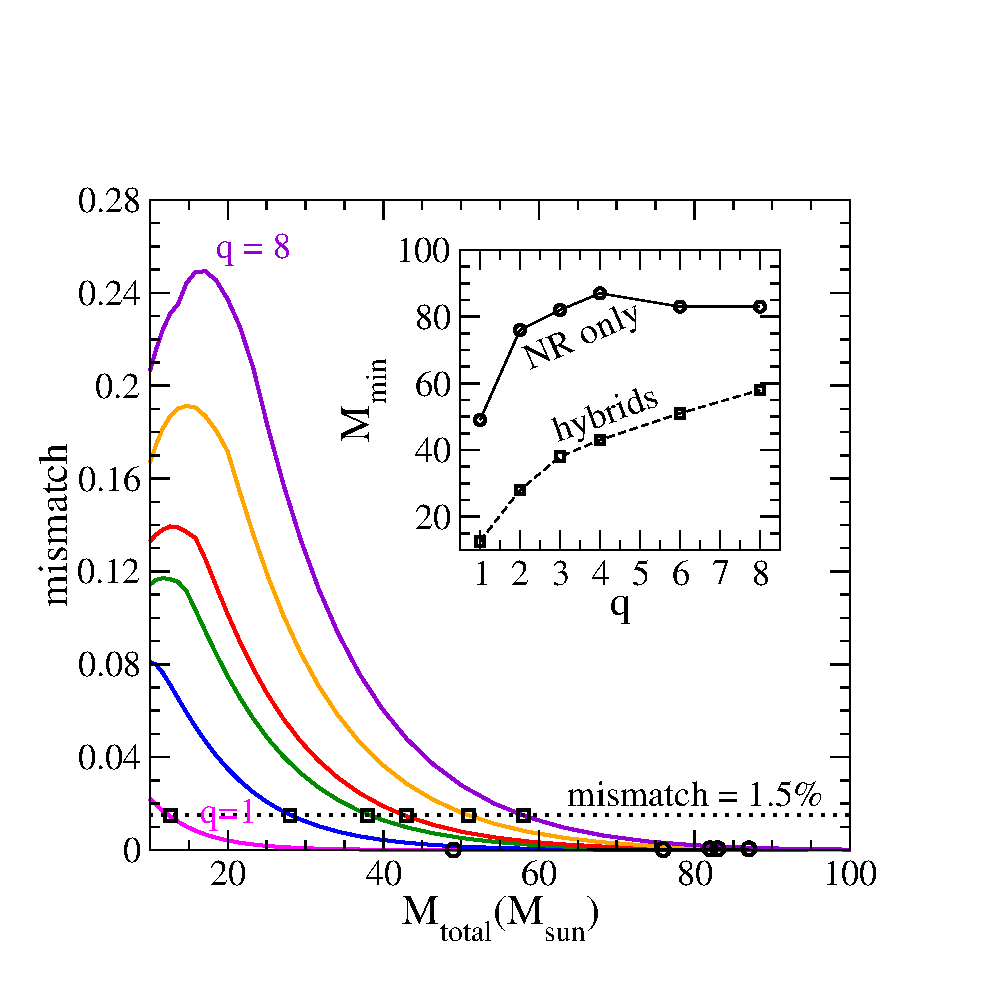
\includegraphics[width=0.9\columnwidth, trim=20 17 75 75]{figures/nrhybbank/maxmismatchVSmass_allq.pdf}
\caption{\label{fig:Current-NR-PN-Errors}Bounds on mismatches of PN-NR
  hybrid waveforms, for the currently existing NR simulations. The PN
  error is for hybrids matched at $M\omega_m=0.025$ for $q=1$,
  $M\omega_m=0.038$ for $q=2$, and $M\omega_m=0.042$ for
  $q=3,4,6,8$. The black circles indicate the lower bound of the
  template bank in Table~\ref{table:etalist4}. The black square show the
  lower bound with a hybrid error of 1.5\%. The inset shows these
  lower bounds as a function of mass ratio.} 
\end{figure}

%\textcolor{red}{Details of hybrids and how we estimate their errors?}\newline
The hybrids we use are constructed by joining the PN and NR portions, as 
described in Sec.~\ref{s2:NRpNhybridwaveforms}. The number of orbits before 
merger at which they are joined depends on the length of the available NR 
waveforms. We estimate the PN waveform errors using hybridization
mismatches $\Gamma_\Hyb$, as discussed in Sec.~\ref{s1:quantifyingerrors}. 
Fig.~\ref{fig:Current-NR-PN-Errors} shows the same for all the hybrids, as a 
function of total mass. In terms of orbital frequency, these are
matched at $M\omega_m=0.025$ for $q=1$, $M\omega_m=0.038$ for $q=2$,
and $M\omega_m=0.042$ for $q=3,4,6,8$. In terms of number of orbits
before merger, this is 26.9 orbits for $q=1$, 13.6 orbits for $q=2$,
12.6 orbits for $q=3$, 14.3 orbits for $q=4$, 17.8 orbits for $q=6$,
and 21.4 orbits for $q=8$. The dotted line indicates a mismatch of
$1.5\%$, a comparatively tight bound that leaves flexibility to accommodate
errors due to template bank discreteness. The black circles show the hybrid
mismatches at the lower mass bound of the NR-only template bank in
Table~\ref{table:etalist4}, which are negligible. The inset shows this minimum 
mass as a function of mass ratio, as well as the minimum attainable mass if we
accept a hybrid error of $1.5\%$. At lower masses, the mismatches increase
sharply with more of the PN part moving into the Advanced LIGO sensitivity band.
This is due to the nature of the frequency dependence of the detector 
sensitivity. The detectors will be most sensitive in a comparatively
narrow frequency band. As the hybridization frequency sweeps through this band, 
the hybrid errors rise sharply. They fall again at the lowest masses, for which
mostly the PN portion stays within the sensitive band.


\begin{figure*}
\begin{center}
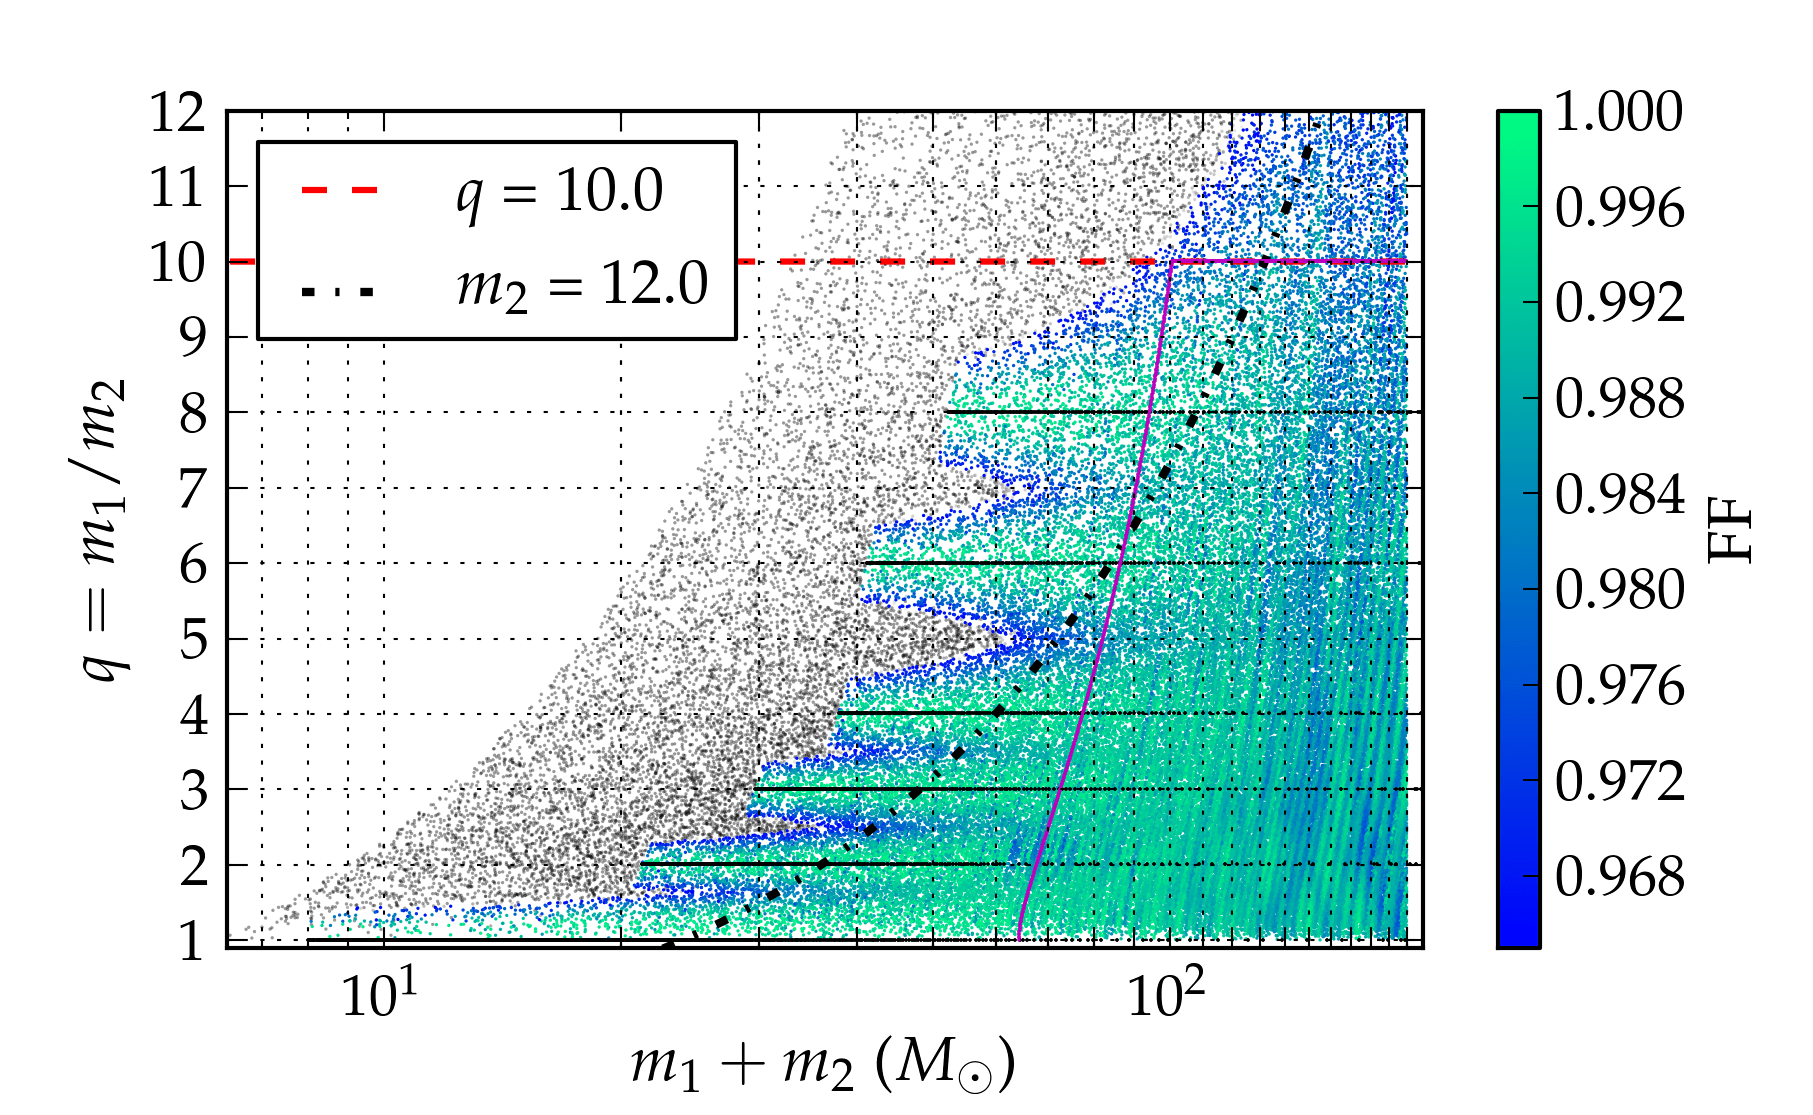
\includegraphics[width=0.8\columnwidth]{figures/nrhybbank/bank001_lowM_01_stochastic_mtot200_logMq_NOhybMM-tiny.png}
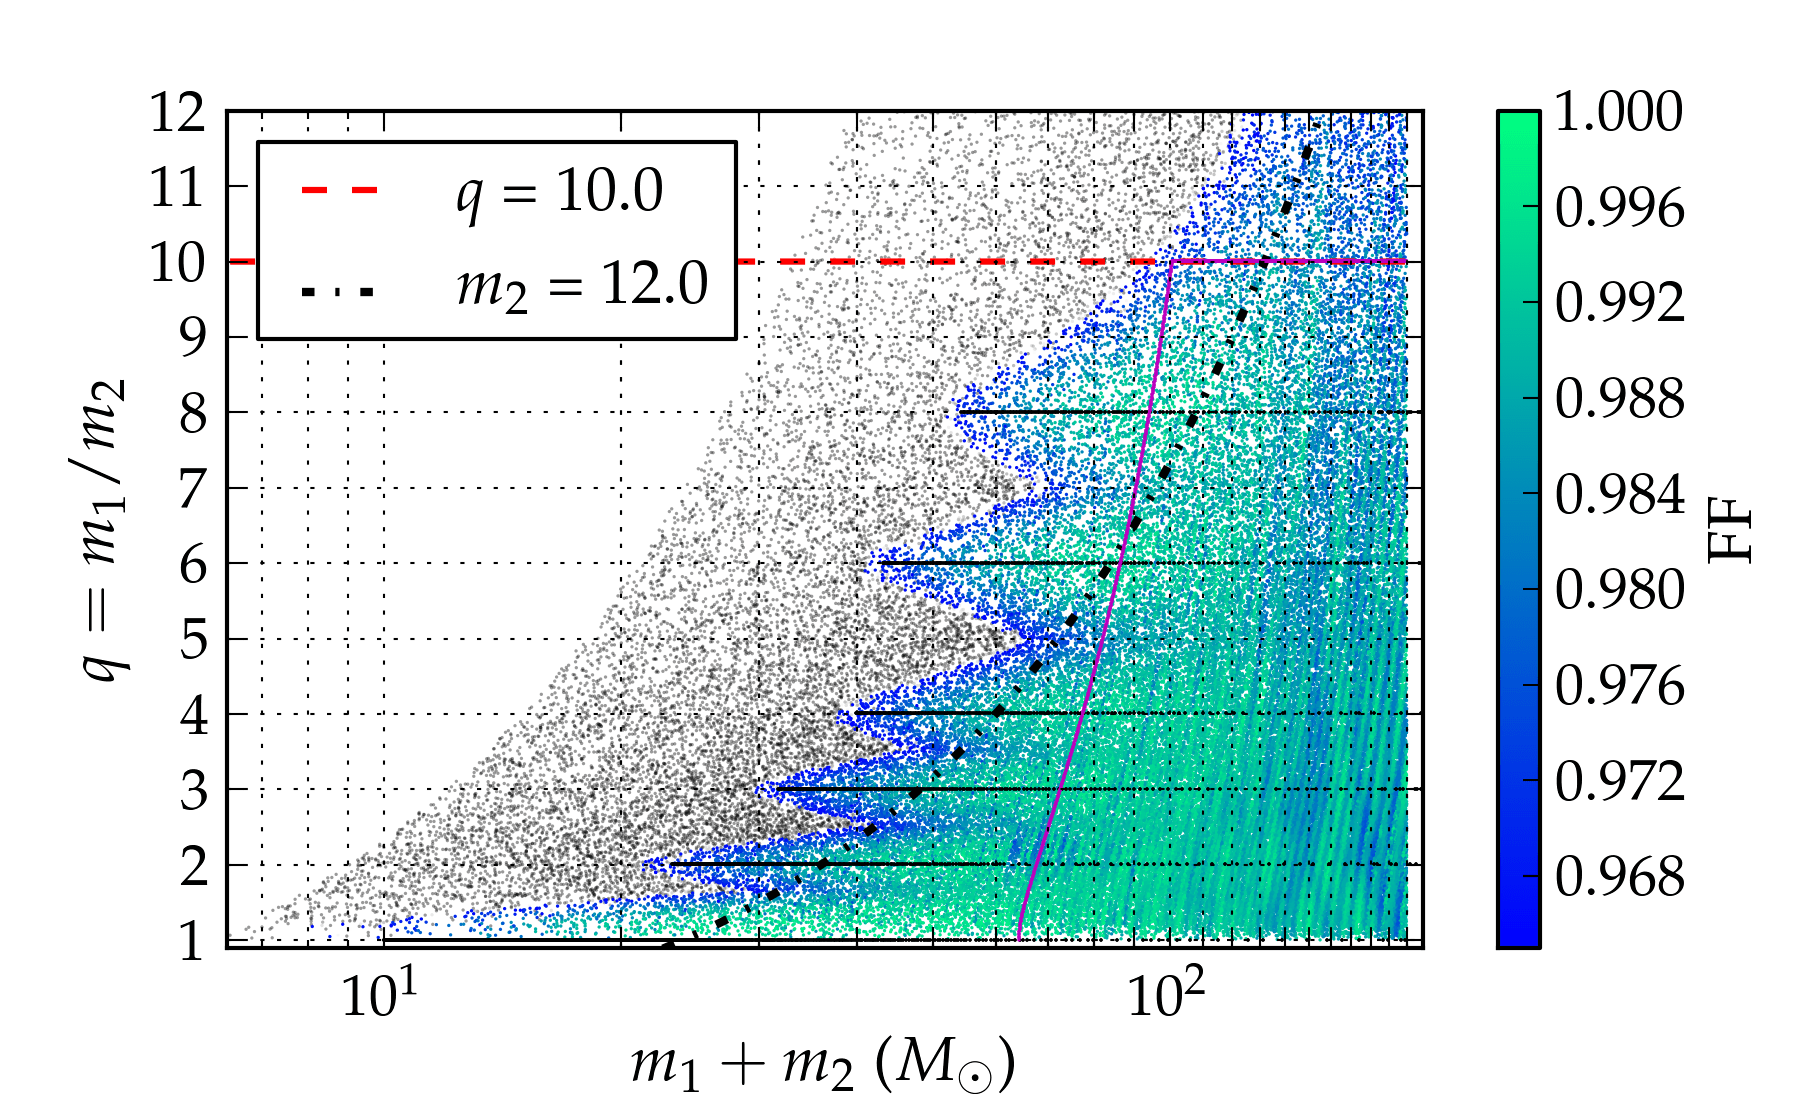
\includegraphics[width=0.8\columnwidth]{figures/nrhybbank/bank001_lowM_01_stochastic_mtot200_logMq_hybMM-tiny.png}
\caption{\label{fig:Current-hybrids-stochastic-FF}These figures show fitting
  factors $\FF$ obtained when using a discrete mass-ratio template bank for
  $q=1,2,3,4,6,8$. For each mass-ratio, the templates are extended down 
  to a total mass where the NR-PN hybridization mismatch becomes
  $3\%$. The bank is placed using the stochastic algorithm, similar to 
  Ref.~\cite{Harry:2009ea,Ajith:2012mn,Manca:2009xw}. 
  The black dots show the location
  of the templates. The fitting factor on the top plot does 
  {\em not} take into account the hybridization error, and therefore shows the
  effect of the sparse placement of the templates alone. 
  The bottom plot accounts for the hybridization error
  and gives the actual fraction of the optimal SNR that would be recovered
  with this bank of NR-PN hybrid templates. The region bounded by the magenta 
  (solid) line in both plots indicates the lower end of the coverage of the 
  bank of un-hybridized NR waveforms. Lastly, the shaded grey dots show the 
  points where the fitting factor was below $96.5\%$.}
\end{center}
\end{figure*}
\begin{figure*}
\begin{center}
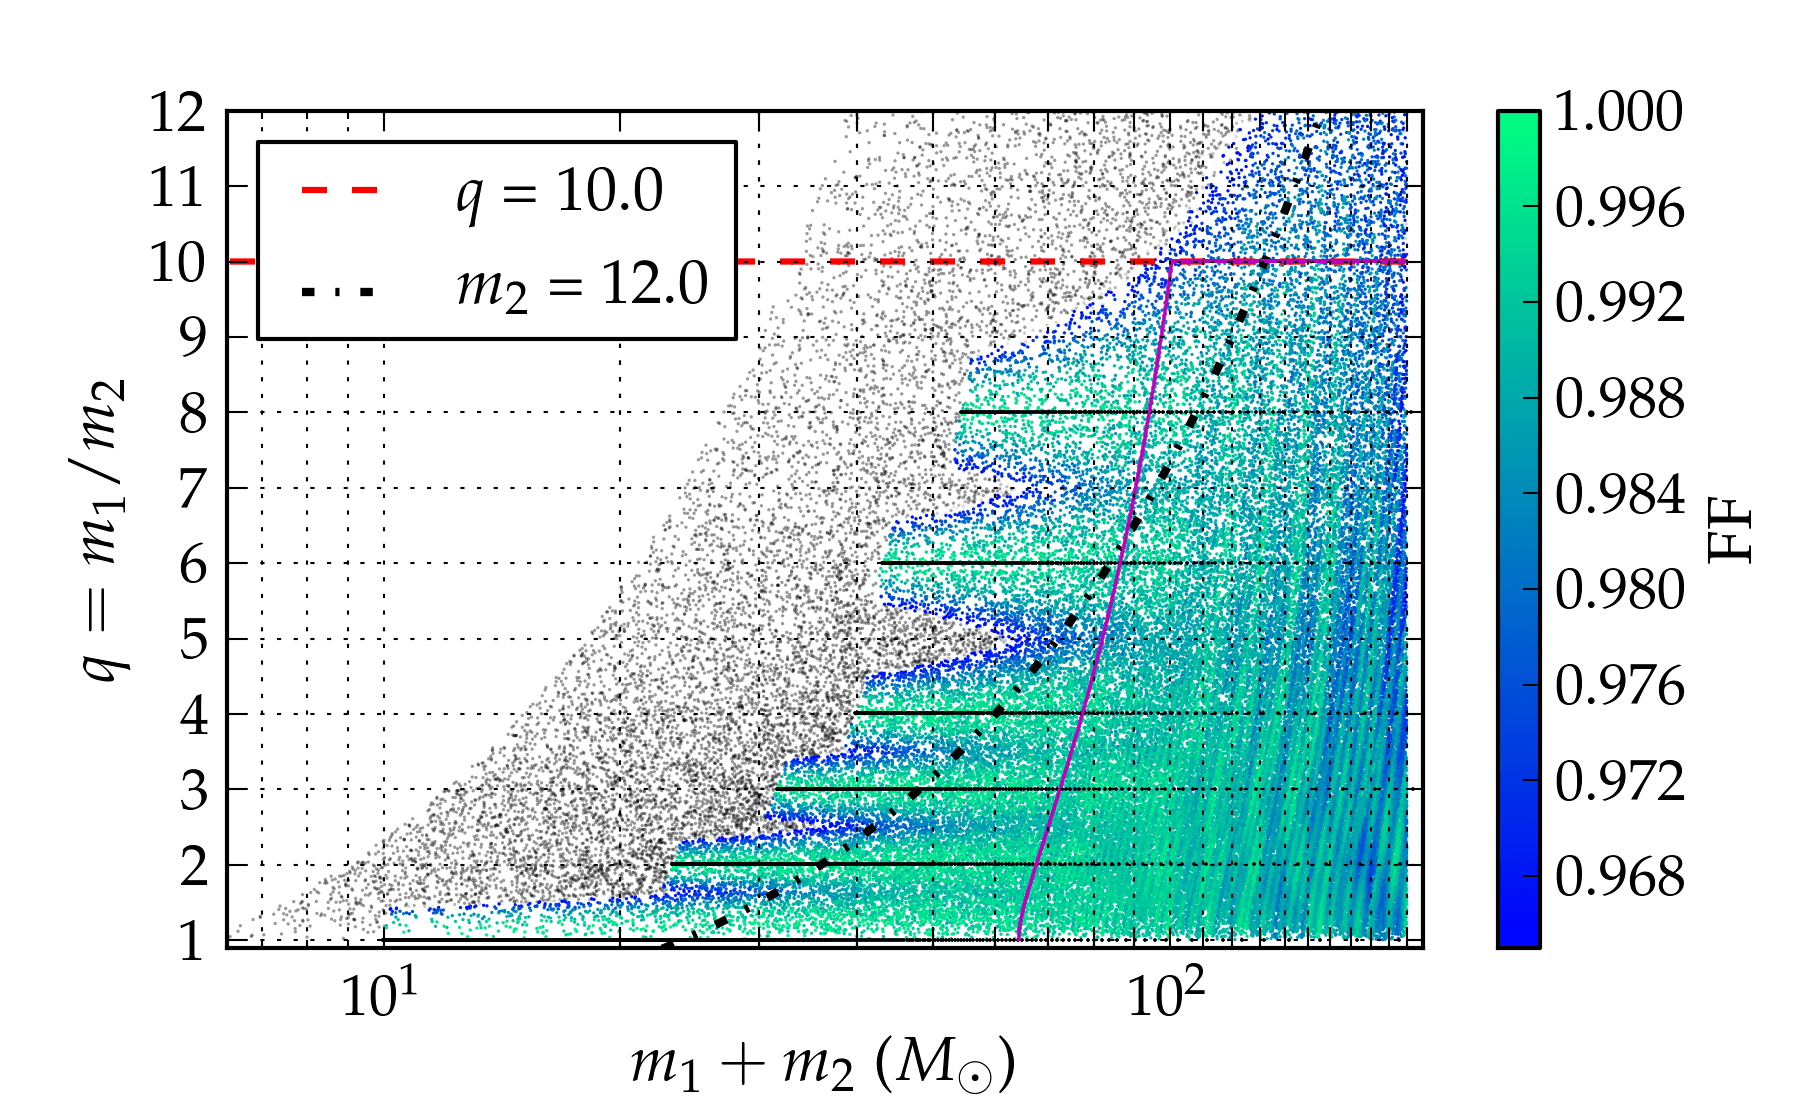
\includegraphics[width=0.8\columnwidth]{figures/nrhybbank/bank_26022013_02_mtot200_logMq_NOhybMM-tiny.png}
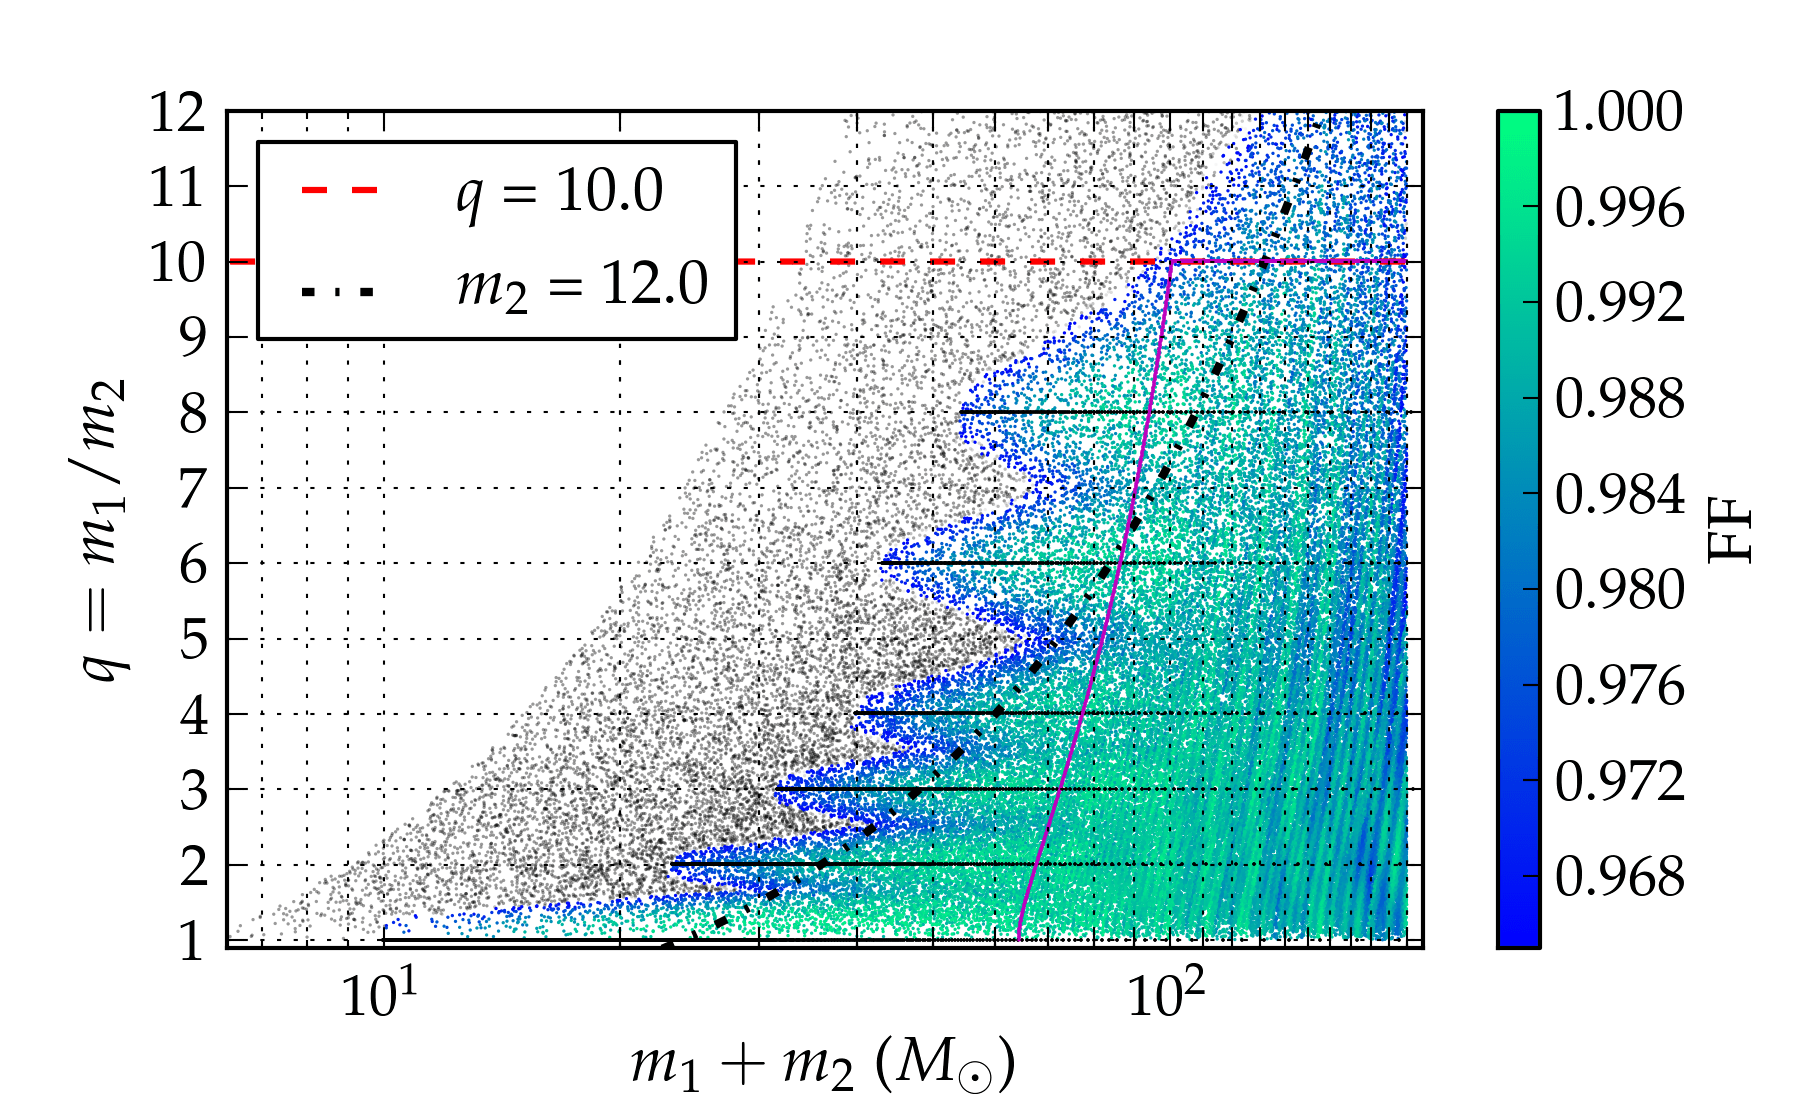
\includegraphics[width=0.8\columnwidth]{figures/nrhybbank/bank_26022013_02_mtot200_logMq_hybMM-tiny.png}
\caption{\label{fig:Current-hybrids-FF}These figures are similar to 
  Fig.~\ref{fig:Current-hybrids-stochastic-FF}. The figures show fitting
  factors $\FF$ obtained when using a discrete mass-ratio template bank for
  $q=1,2,3,4,6,8$. For each mass-ratio, the templates are extended down 
  to a total mass where the NR-PN hybridization mismatch becomes
  $3\%$. Templates are placed independently for each mass-ratio, and span the 
  full range of total masses. For each mass-ratio, neighboring templates are 
  required to have an overlap of $97\%$. The union of the six single-$q$ 
  one-dimensional banks is taken as the final bank. The black dots show the 
  location of the templates. The fitting factor on the top plot does 
  {\em not} take into account the hybridization error, and therefore shows the
  effect of the sparse placement of the templates alone. The bottom plot accounts
  for the hybridization error
  and gives the actual fraction of the optimal SNR that would be recovered
  with this bank of NR-PN hybrid templates. The region bounded by the magenta 
  (solid) line in both plots indicates the lower end of the coverage of the 
  bank of un-hybridized NR waveforms. Lastly, the shaded grey dots show the 
  points where the fitting factor was below $96.5\%$.}
\end{center}
\end{figure*}

\begin{figure*}
\begin{center}
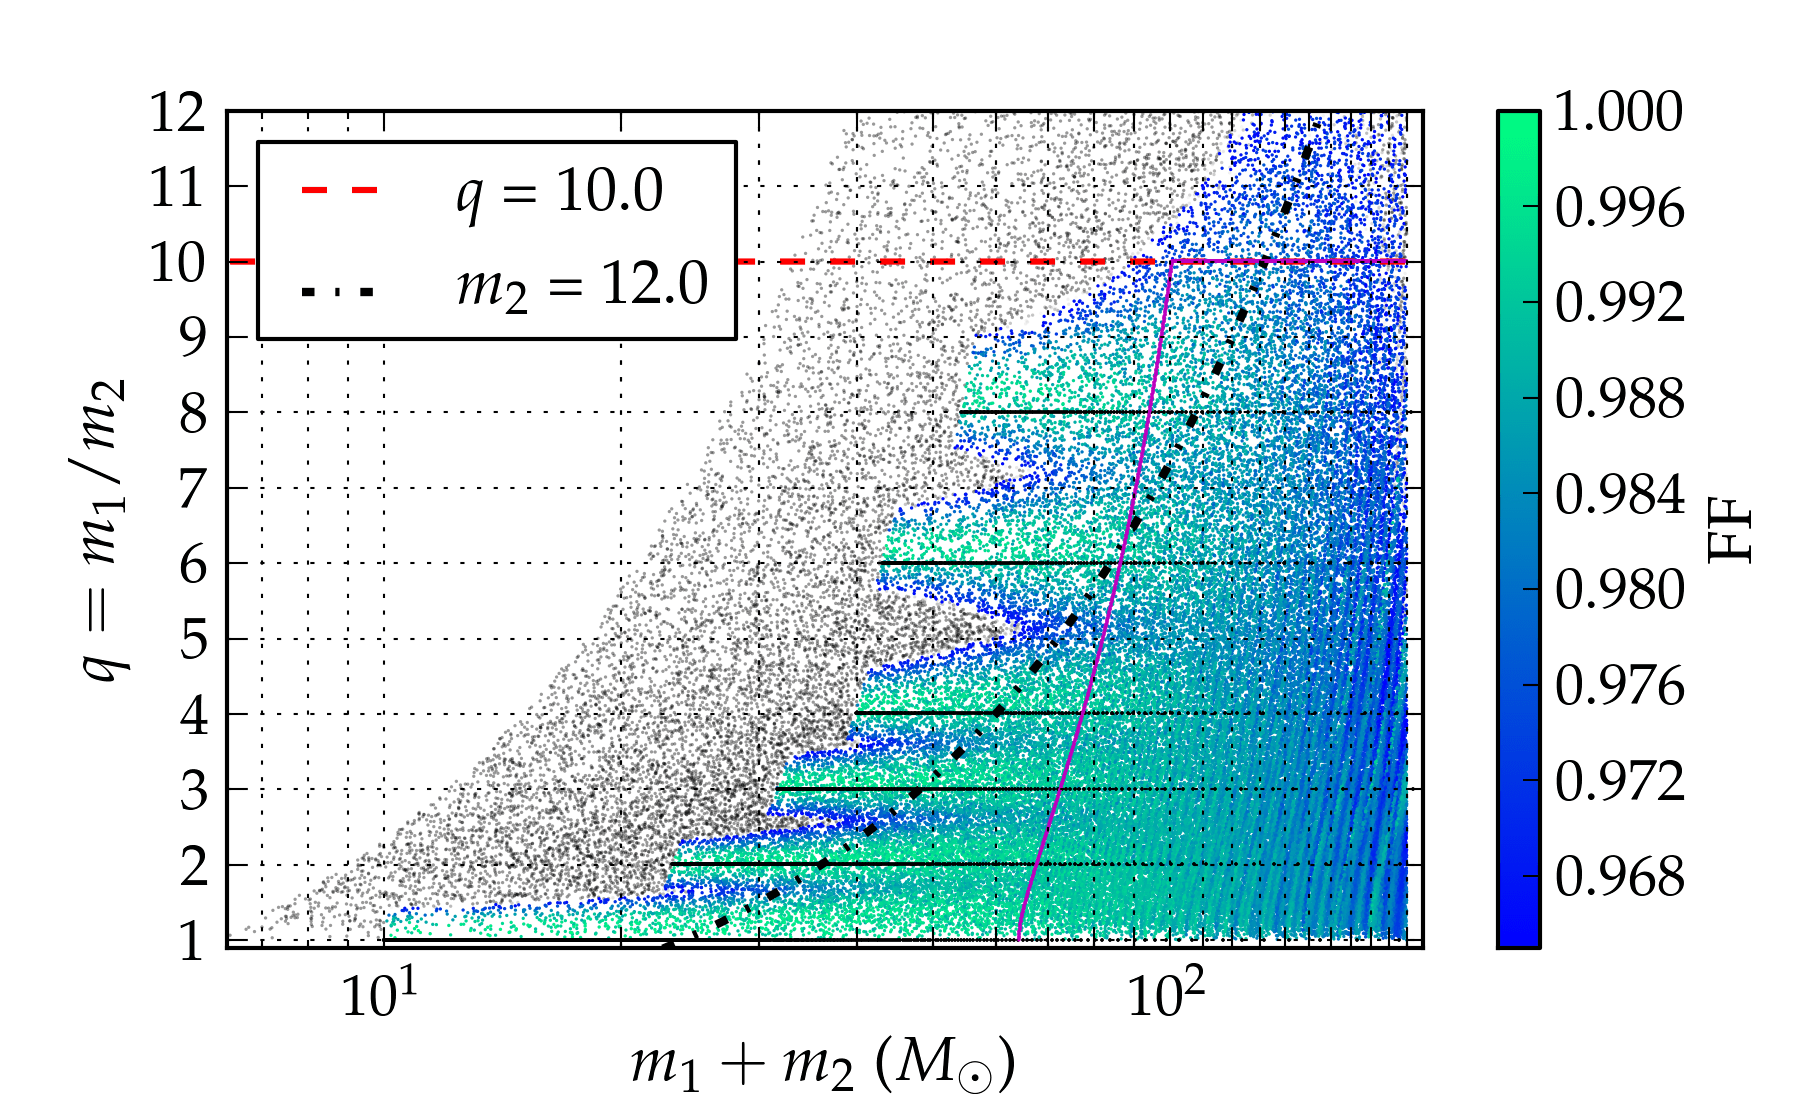
\includegraphics[width=0.8\columnwidth]{figures/nrhybbank/bank_26022013_02_hybrids_mtot200_logMq_NOhybMM-tiny.png}
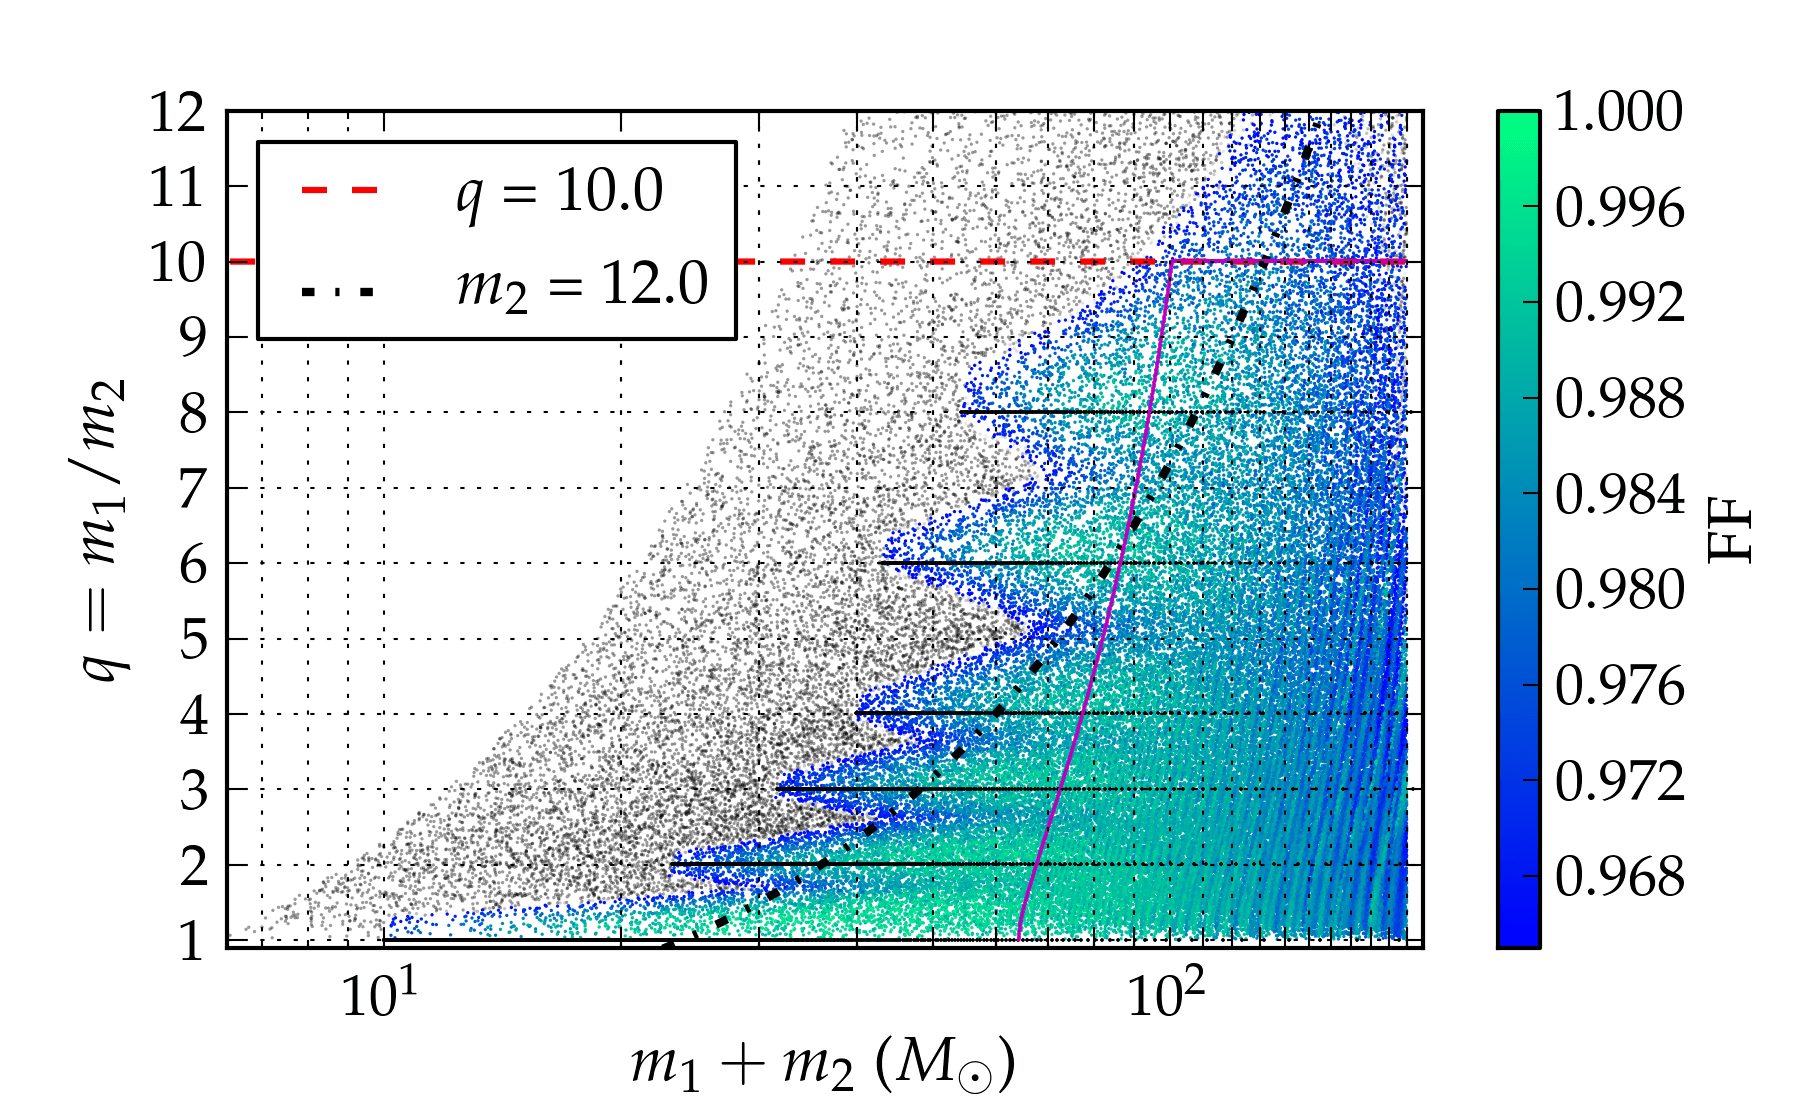
\includegraphics[width=0.8\columnwidth]{figures/nrhybbank/bank_26022013_02_hybrids_mtot200_logMq_hybMM-tiny.png}
\caption{\label{fig:Current-real-hybrids-FF}This figure is similar to 
  Fig.~\ref{fig:Current-hybrids-FF}. The figures show fitting
  factors $\FF$ obtained when using a discrete mass-ratio template bank for
  $q=1,2,3,4,6,8$. Templates are placed independently for each mass-ratio, and 
  span the range of total masses, down to the region where the hybrid errors
  become $3\%$. For each mass-ratio, neighboring templates are 
  required to have an overlap of $97\%$. The union of the six single-$q$ 
  one-dimensional banks is taken as the final bank. The black dots show the 
  location of the templates. The GW signals are modeled using the EOBNRv2
  approximant~\cite{BuonannoEOBv2Main}, while TaylorT4+NR hybrids are used as
  templates. The fitting factor on the left plot shows the combined effect of 
  the sparse placement of the templates, and the (relatively small) 
  disagreement between the hybrid and EOBNRv2 waveforms. The right plot
  explicitly accounts for the hybridization error and gives the (conservative)
  actual fraction of the optimal SNR that would be recovered
  with this bank of NR-PN hybrid templates. The region bounded by the magenta 
  (solid) line in both plots indicates the lower end of the coverage of the 
  bank of un-hybridized NR waveforms. Lastly, the shaded grey dots show the 
  points where the fitting factor was below $96.5\%$.  }
\end{center}
\end{figure*}

%\textcolor{red}{How do we construct the stochastic bank, and how well does it perform?}\newline
We now consider template banks viable for hybrids constructed from currently 
available NR waveforms at mass ratios $q=1,2,3,4,6,8$. The lower mass limit,
in this case, is extended down to masses where the hybridization error 
exceeds $3\%$. We demonstrate two independent methods of laying
down the bank grid. First, we use the stochastic placement method that proceeds
as described in Sec.~\ref{s1:NRonlybank}. The templates are sampled over the
total mass - mass-rato $(M,q)$ coordinates, sampling $q$ from the restricted
set. The total mass $M$ is sampled from the continuous interval between the 
lower mass limit, which is different for each $q$, and the upper limit of
$200M_\odot$. To assess the SNR loss from the sparse placement
of the templates, we simulate a population of $100,000$ BBH signal waveforms,
with masses sampled with $3M_\odot\leq m_{1,2}\leq 200M_\odot$ and 
$M\leq 200M_\odot$, and filter them through the bank. This portion of the SNR
loss needs to be measured with both signals and templates in the same waveform
manifold. We use the EOBNRv2 approximant~\cite{BuonannoEOBv2Main} to model both, 
as it has been calibrated to most of the NR waveforms we consider here, and it
allows us to model waveforms for arbitrary systems. The left panel of
Fig.~\ref{fig:Current-hybrids-stochastic-FF} shows the
fraction of the optimal SNR that the bank recovers, accounting for its 
discreteness alone. We observe that, with just six mass-ratios, the bank 
can be extended to much lower masses before it is limited by the restricted
sampling of mass-ratios for the templates. For binaries with both black-holes 
more massive than $\sim 12M_\odot$, the spacing between mass-ratios was found 
to be sufficiently dense. The total SNR loss, after subtracting out 
the hybrid mismatches from Fig.~\ref{fig:Current-NR-PN-Errors}, are shown in 
the right panel of Fig.~\ref{fig:Current-hybrids-stochastic-FF}. 
At the lowest masses, the coverage shrinks between the lines of constant $q$ 
over which the templates are placed, due to the hybrid errors increasing 
sharply. We conclude that this bank is viable for hybrid templates for GW 
searches for BBHs with $m_{1,2}\geq 12M_\odot$, $1\leq q\leq 10$, and 
$M\leq 200M_\odot$. Over this region the bank will recover more than $96.5\%$
of the optimal SNR. This is a significant increase over the coverage allowed 
for with the purely-NR bank, the region of coverage of which is shown in the 
right panel of Fig.~\ref{fig:Current-hybrids-FF}, bounded at lowest masses by 
the magenta (solid) curve.


%\textcolor{red}{What is the second method, why do we use it, and how well does it compare?}\newline
Second, we demonstrate a non-stochastic algorithm of bank placement, with 
comparable results. We first construct six independent bank grids, each
restricted to one of the mass-ratios $q=1,2,3,4,6,8$, and spanning the full 
range of total masses. The template with the lowest total mass is chosen 
by requiring the hybrid mismatch to be $3\%$ at that point.
The spacing between neighboring templates is
given by requiring that the overlap between them be $97\%$. 
We take the union of these banks as the final 
two-dimensional bank. As before, we measure the SNR loss due to discreteness of
the bank and the waveform errors in the templates separately. To estimate the
former, we simulate a population of $100,000$ BBH systems, and filter
them through the bank. The signals and the templates are both modeled
with the EOBNRv2 model. The left panel of Fig.~\ref{fig:Current-hybrids-FF}
reveals the fraction of SNR recovered over the mass space, accounting for the 
sparsity of the bank alone, i.e. $1-\Gamma_\mathrm{bank}$. At lower masses, 
we again start to see gaps between the lines of constant mass ratio which
become significant at $m_{1,2} \leq 12M_\odot$. 
The right panel of Fig.~\ref{fig:Current-hybrids-FF} shows the final fraction 
of the optimal SNR recovered, i.e. the $\FF$ as defined in Eq.~(\ref{eq:FFGammas}). 
As before, these are computed by subtracting out the hybrid mismatches 
$\Gamma_\Hyb$ in addition to the discrete mismatches, as described in
Sec.~\ref{s1:quantifyingerrors}. 

The efficacy of both methods of template bank construction
can be compared from Fig.~\ref{fig:Current-hybrids-stochastic-FF} and 
Fig.~\ref{fig:Current-hybrids-FF}. We observe that the final banks from either
of the algorithms have very similar SNR recovery, and are both effectual over
the range of masses we consider here. Both were also found to give a very 
similar number of templates. The uniform-in-overlap method yields a grid 
with $2,325$ templates. The stochastic bank, on the other hand, was placed with a
requirement of $98\%$ minimal mismatch, and had $2,457$ templates. 
This however includes templates with $m_{1,2} < 12M_\odot$. Restricted
to provide coverage over the region with $m_{1,2}\geq 12M_\odot$, $1\leq q\leq 10$,
and $M\leq 200M_\odot$, the two methods yield banks with $627$ and $667$
templates respectively. The size of these banks is comparable to one 
constructed using the second-order post-Newtonian TaylorF2 hexagonal 
template placement method~\cite{SathyaBankPlacementTauN,BabaketalBankPlacement,
SathyaMetric2PN,Cokelaer:2007kx}, 
which yields a grid of $522$ and $736$ templates, for a minimal
match of $97\%$ and $98\%$, respectively.

%\textcolor{red}{How do we show the robustness of the banks using NR hybrids?}\newline
Finally, we test the robustness of these results using TaylorT4+NR hybrids 
as templates. As before, we simulate a population of $100,000$ BBH signal 
waveforms. As we do not have hybrids for arbitary binary
masses, we model the signals as EOBNRv2 waveforms. This population is filtered
against a bank of hybrid templates. The SNR recovered is shown in the left 
panel of Fig.~\ref{fig:Current-real-hybrids-FF}. Comparing with the left panels 
of Fig.~\ref{fig:Current-hybrids-stochastic-FF},~\ref{fig:Current-hybrids-FF}, 
we find that the EOBNRv2 manifold is a reasonable approximation for the hybrid 
manifold; and that, at lower masses, there is a small systematic bias in the 
hybrids towards EOBNRv2 signals with slightly higher mass-ratios.
The right panel of Fig.~\ref{fig:Current-real-hybrids-FF} 
shows the fraction of optimal SNR recovered after subtracting out the hybrid
mismatches from the left panel. The similarity of the $\FF$ distribution between 
the right panels of Fig.~\ref{fig:Current-real-hybrids-FF} and 
Fig.~\ref{fig:Current-hybrids-stochastic-FF},~\ref{fig:Current-hybrids-FF}
is remarkable. This gives us confidence that the EOBNRv2 model is a good 
approximation for testing NR/hybrid template banks, as we do in this chapter; 
and that a template bank of NR+PN hybrids is indeed effectual for binaries 
with $m_{1,2}\geq 12M_\odot$, $M\leq 200M_\odot$ and $q\leq 10$.



\section{Complete NR-PN hybrid bank for non-spinning BBH}\label{s1:futureNRpNhybridbank}

\begin{figure*}
\begin{center}
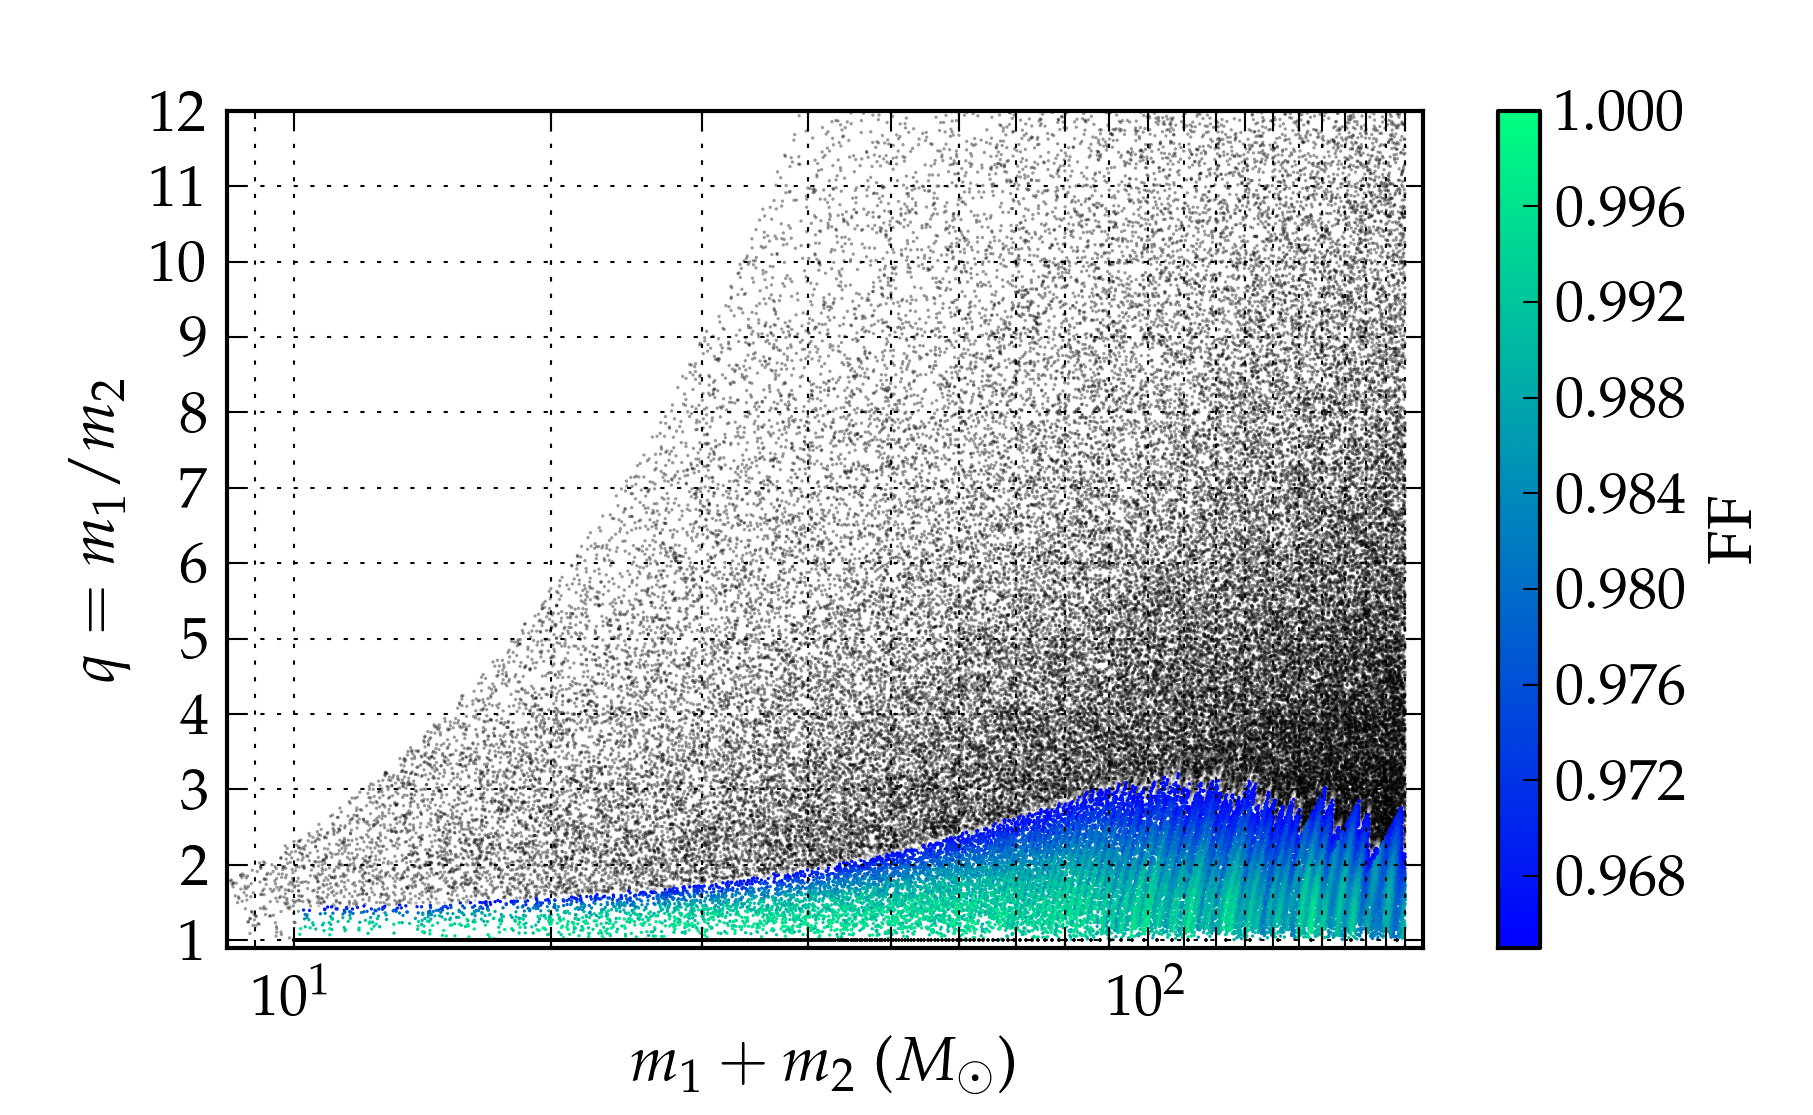
\includegraphics[width=0.7\columnwidth]{figures/nrhybbank/bank_separate_q1_mtot200_match-tiny.png}
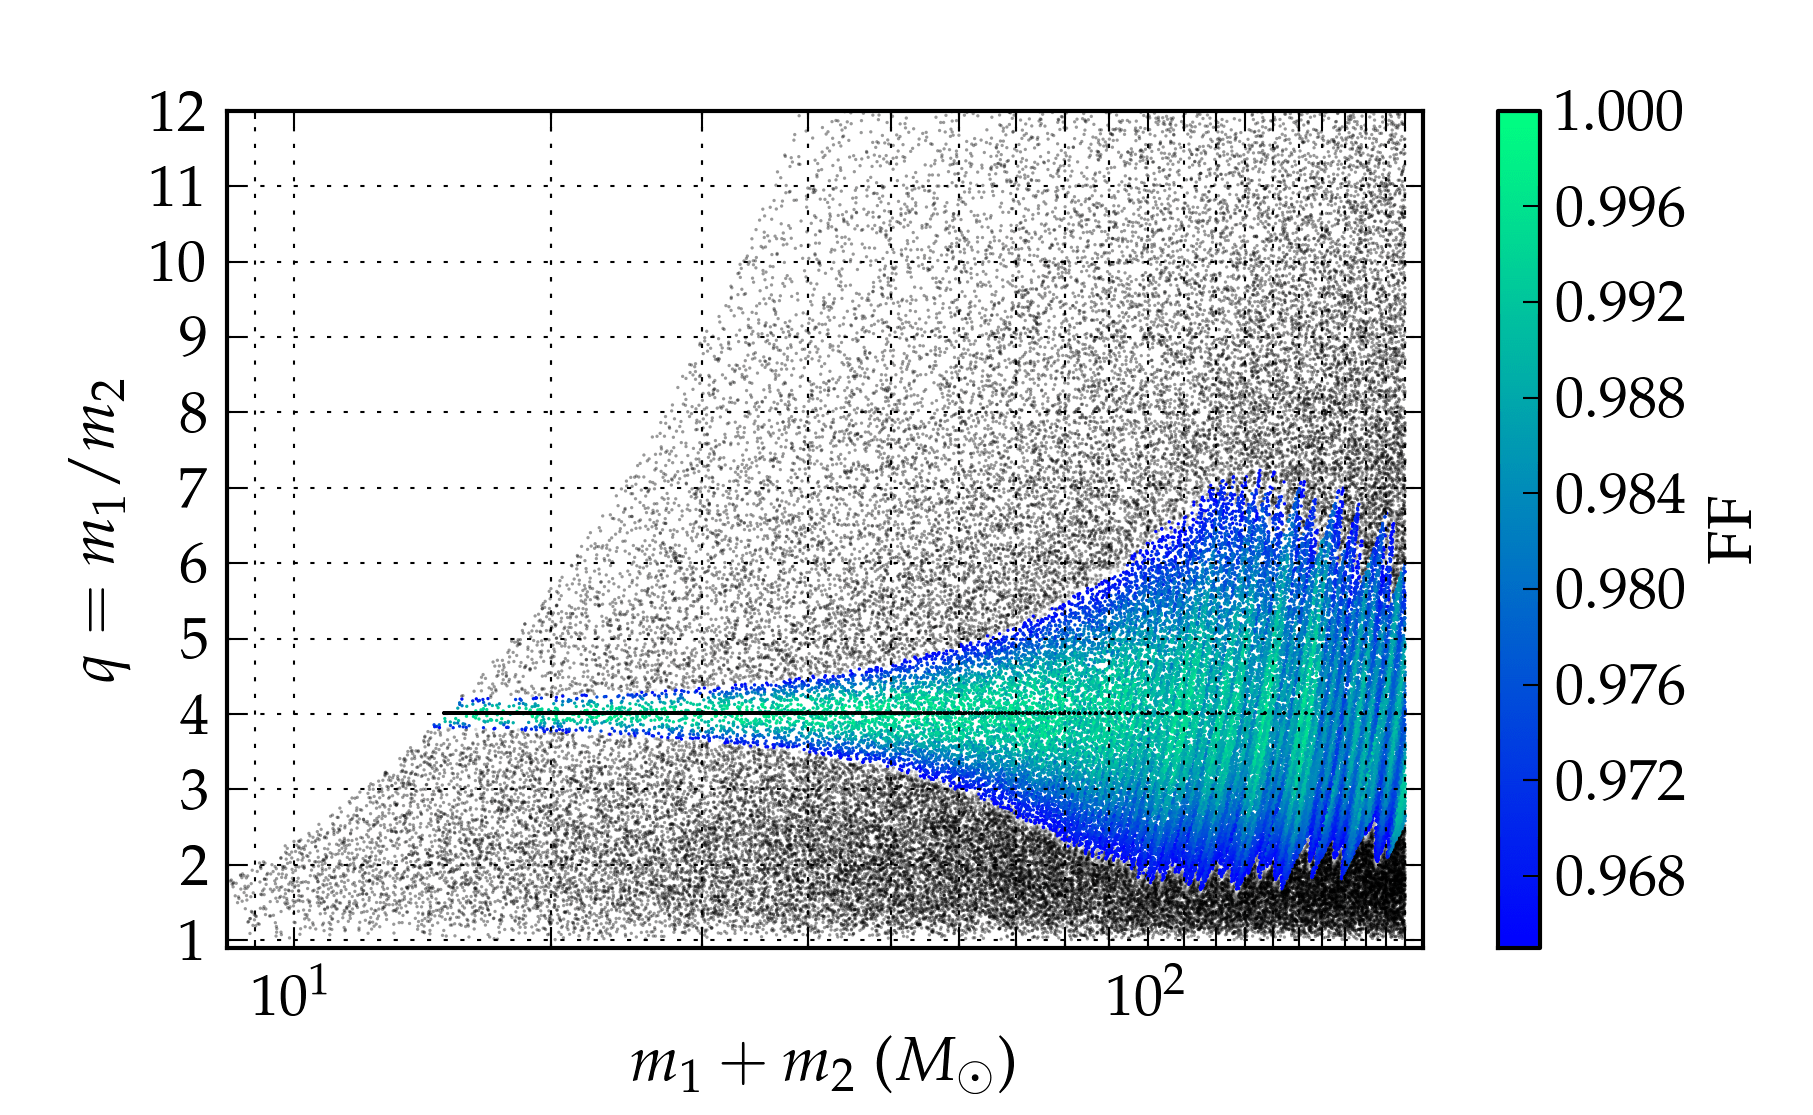
\includegraphics[width=0.7\columnwidth]{figures/nrhybbank/bank_separate_q4_mtot200_match-tiny.png}
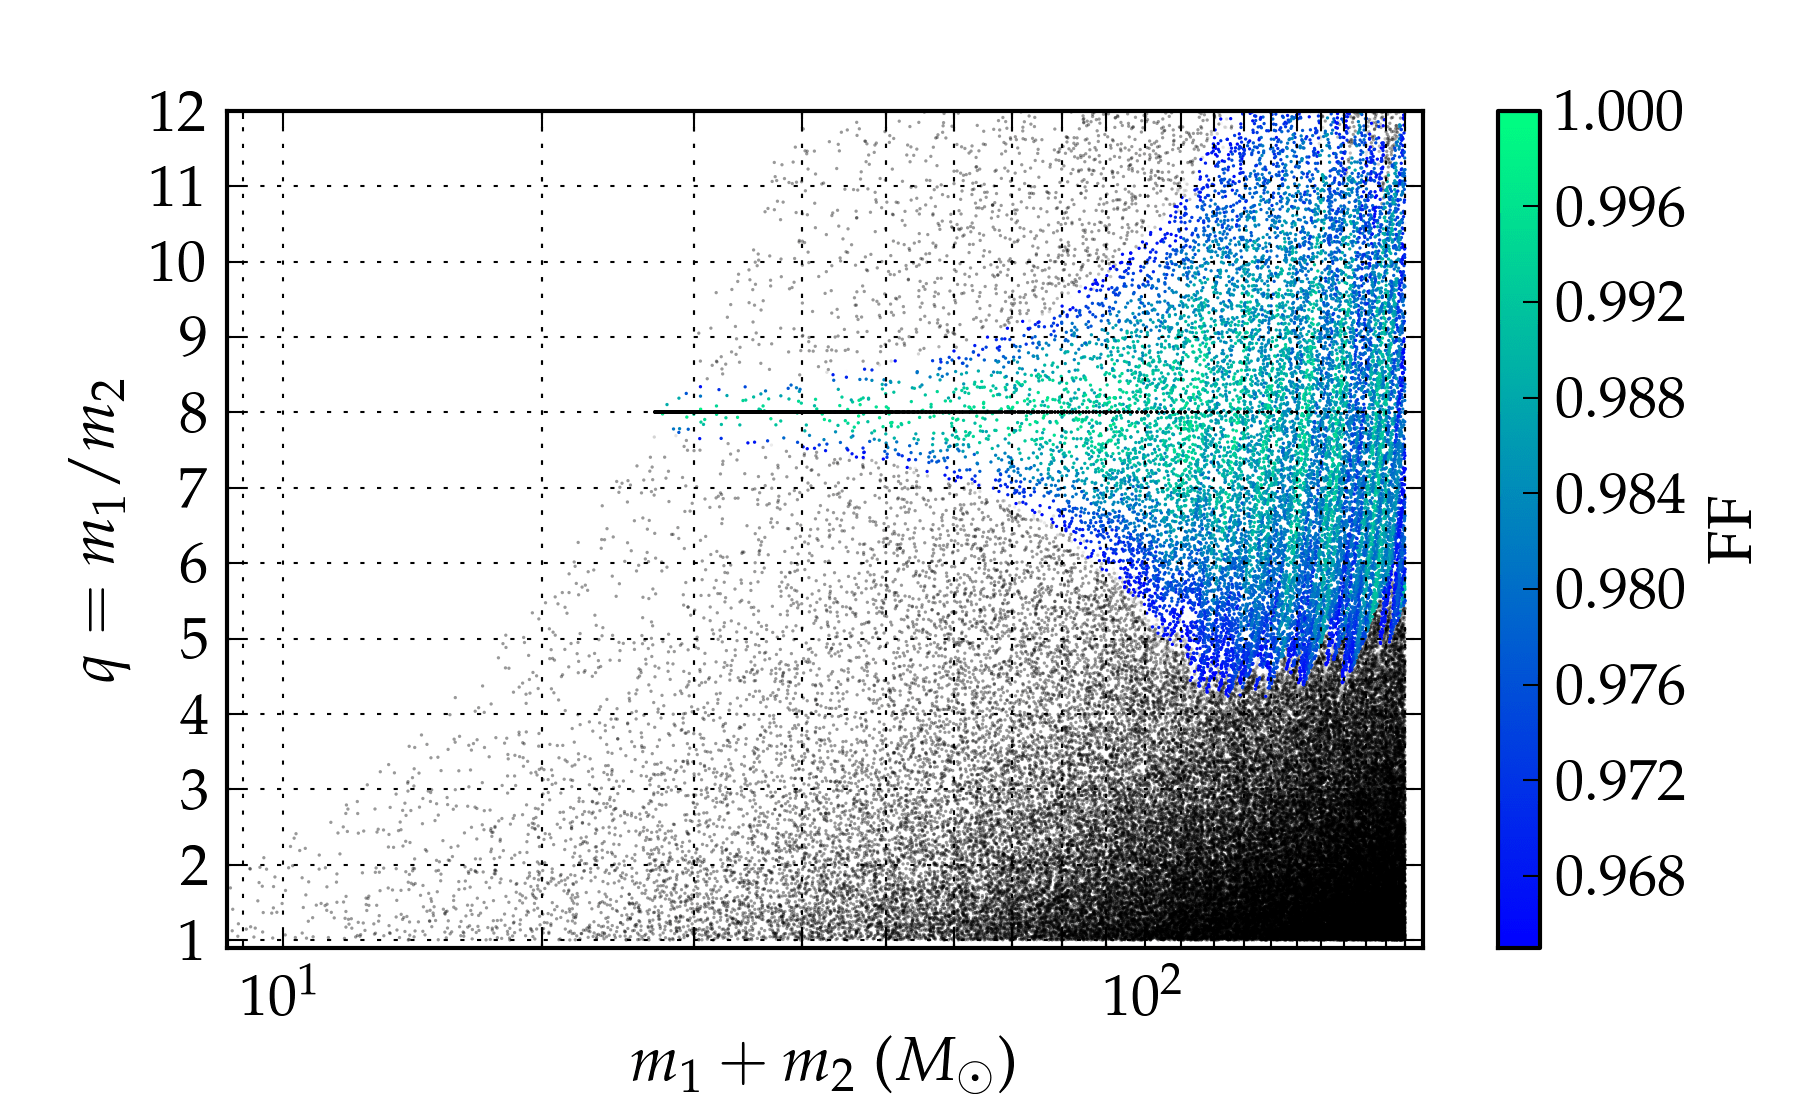
\includegraphics[width=0.7\columnwidth]{figures/nrhybbank/bank_separate_q8_mtot200_match-tiny.png}
\caption{\label{fig:separate_q148} These figures show the coverage of template
  banks restricted to single mass-ratios, i.e. (from top to bottom) 
  $q = 1, 4, 8$. We note that at 
  higher total masses, the templates are correlated to simulated signals for
  considerably different mass-ratios, than at lower total masses. This agrees
  with what we expect as with decreasing total mass, the number of cycles in
  the sensitive frequency band of Advanced LIGO increases.} 
\end{center}
\end{figure*}

%\textcolor{red}{Why do we need to extend the bank and where?}\newline
The last sections outlined properties of template banks of NR
waveforms (and their hybrids) which are available today. 
We also investigate the parameter and length requirements for future NR 
simulations, that would let us contruct detection template banks all the
way to $M=m_1+m_2=12M_\odot$. This lower limit was chosen following 
Ref.~\cite{Brown:2012nn,CompTemplates2009} which showed that the region with
$M\lesssim 12M_\odot$ can be covered with banks of post-Newtonian inspiral-only
waveforms.

%\textcolor{red}{Outline how we constructing the future-bank.}\newline
Constructing such a bank is a two-step process.  First, we pick mass-ratios 
that allow construction of such a bank given long enough waveforms for these
mass-ratios. Second, one needs to determine the necessary length of the NR 
portion of the waveforms, such that the PN-hybridization error is sufficiently
low for all masses of interest.

To motivate the first step, Fig.~\ref{fig:separate_q148} shows the coverage of
banks that sample from a {\em single} mass-ratio each (from left to right: $q=1,4,8$). We see that the resolution
in $q$ required at lower values of $M$ increases sharply below 
$M\sim 60M_\odot$. This follows from the increase in the number of waveform
cycles in aLIGO frequency band as the total mass decreases, which, in turn,
increases the discriminatory resolution of the matched-filter along the $q$ axis.
\begin{figure*}
\begin{center}
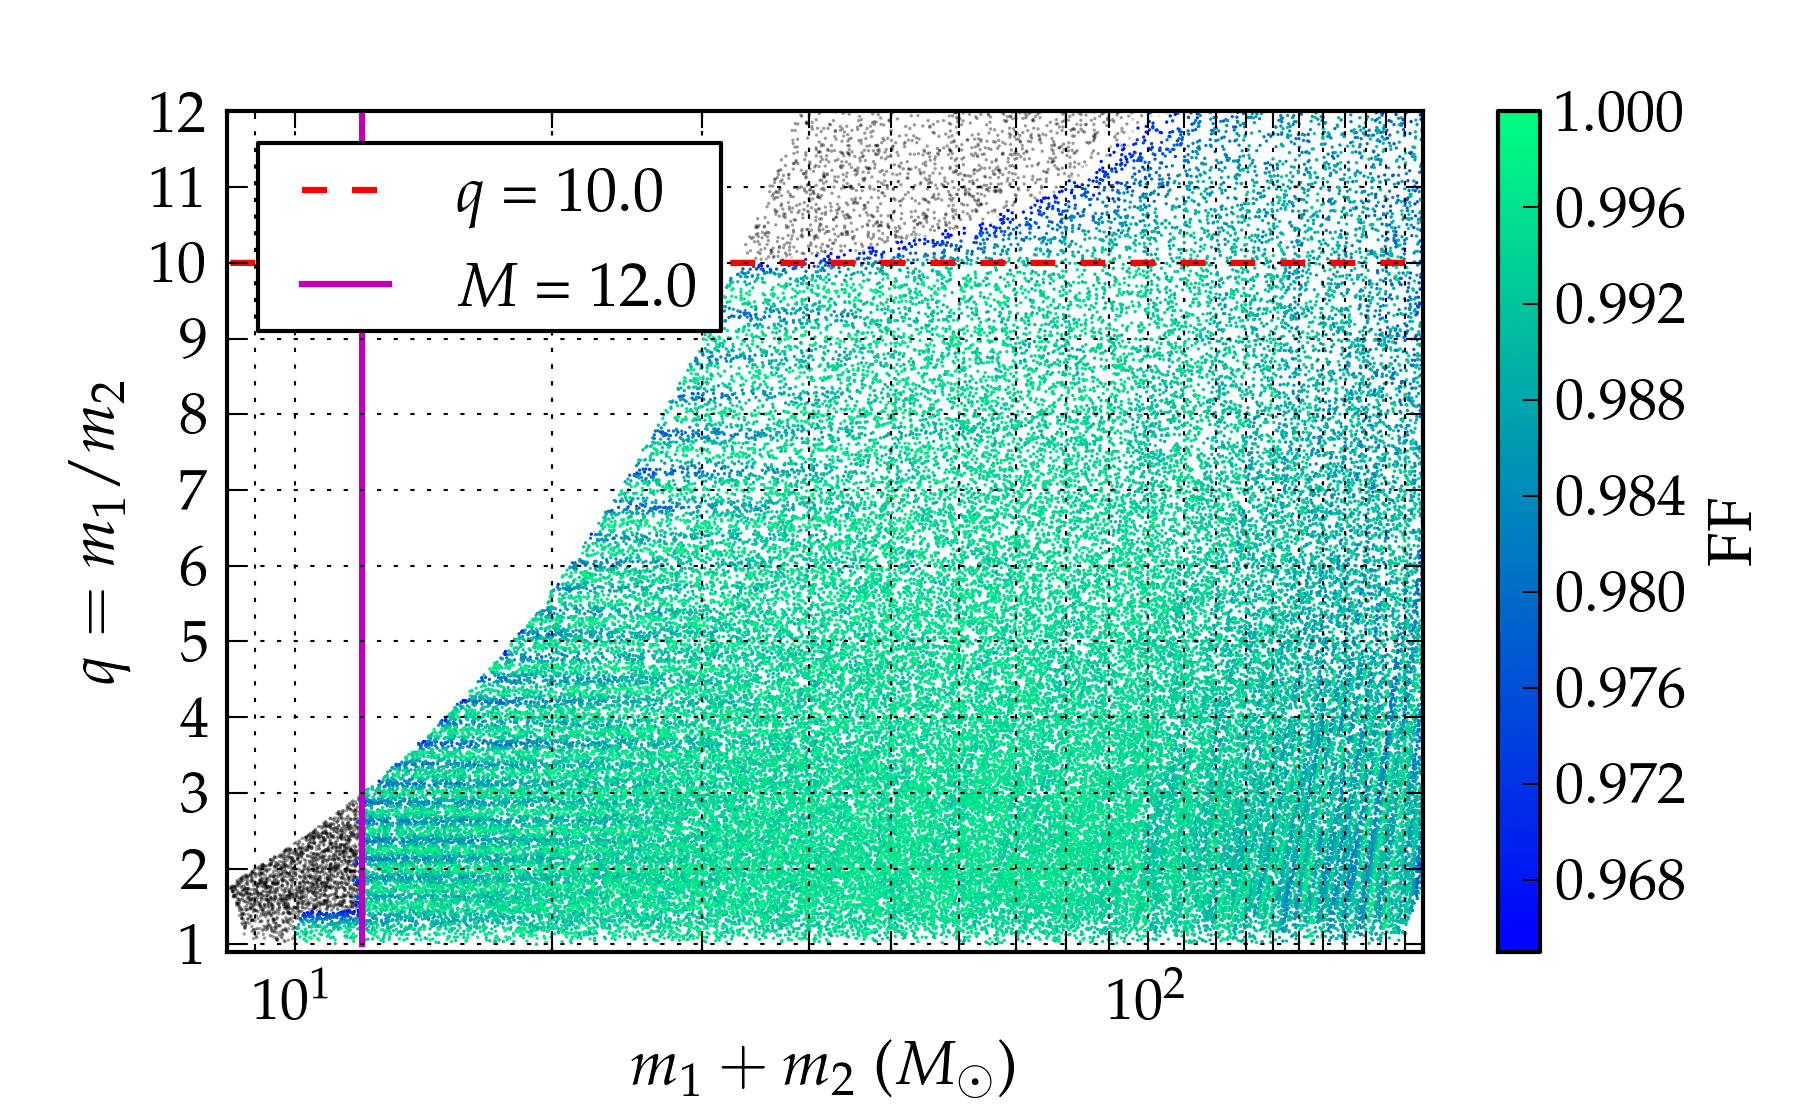
\includegraphics[width=0.8\columnwidth]{figures/nrhybbank/bank_seperate_q1-4-35-4-65-9-6_01_mtot200_match-tiny.png}
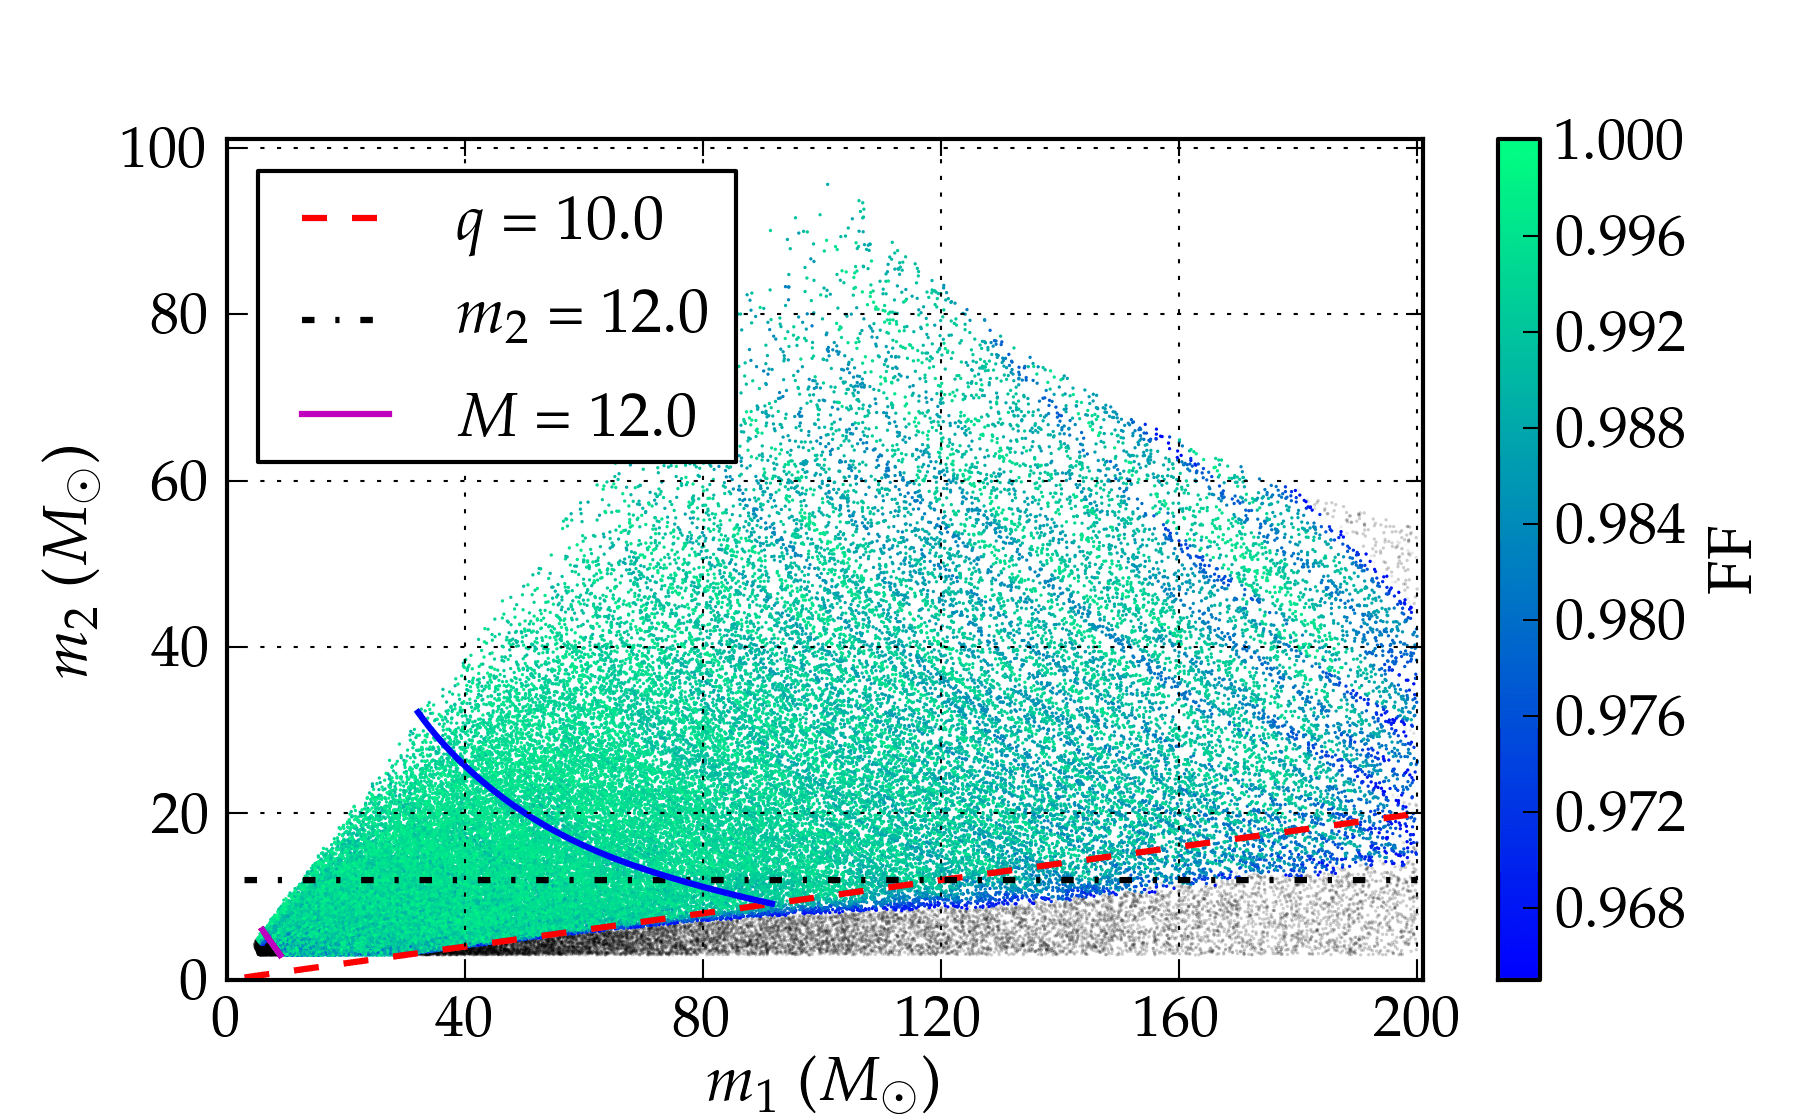
\includegraphics[width=0.8\columnwidth]{figures/nrhybbank/bank_seperate_q1-4-35-4-65-9-6_01_m1m2200_match-tiny.png}
\caption{\label{fig:templatebank_halfMassRatios}This figure shows
  fitting factors for a hybrid template bank which samples from the 26 mass
  ratios $q=1,1.5,1.75,2,..,9.6$, and allows coverage to masses down to 
  $m_1 + m_2 = 12M_{\odot}$ and $1\leq q\leq 10$, with a minimal-match of $98\%$
  at the lowest masses. 
  The left and right panel show the same on $M-q$ and $m_1-m_2$ axes, 
  respectively. The magenta lines, in both panels, shows the upper bound 
  in total mass, below which frequency-domain PN waveforms can be used to construct template banks for aLIGO
  searches~\cite{CompTemplates2009,Brown:2012nn}. The dash-dotted line
  in the right panel shows the lower mass limit on the smaller component object,
  to which a bank of currently available NR-PN hybrids can cover, i.e.
  $\mn(m_1,m_2)=12M_\odot$ (see Sec.~\ref{s1:NRpNhybridbank}). The blue (solid)
  curve in  the right panel gives the lower mass limit to which a bank of
  currently available NR waveforms can cover (see Sec.~\ref{s1:NRonlybank}).
  Thus, between the simulations listed in Table~\ref{table:fullqlist}, 
  and frequency domain PN waveforms, we can search for the entire range of 
  BBH masses.}
\end{center}
\end{figure*}
\begin{table}
\begin{center}
\begin{tabular}{| c |}
\hline
$q\,(\equiv m_1/m_2)$ \\ \hline
1, 1.5, 1.75, \\
2, 2.25, 2.5, 2.75, \\
3, 3.25, 3.5, 3.8, \\
4.05, 4.35, 4.65, 4.95, \\
5.25, 5.55, 5.85, \\
6.2, 6.55, \\
7, 7.5, \\
8, 8.5, \\
9, 9.6 \\
%0.0884 & 9.2 & ?? \\
\hline
\end{tabular}
\caption{List of mass-ratios, a template bank restricted to which will be effectual
over the region of the non-spinning BBH mass space where $m_1+m_2\gtrsim 12M_\odot$
and $1\leq q\leq 10$. The fraction of optimal SNR recovered by such a bank,
accounting for discreteness losses, remains above $98\%$. This is shown in
Fig.~\ref{fig:templatebank_halfMassRatios}.}
\label{table:fullqlist}
\end{center}
\end{table}
To determine the least set of mass-ratios which would sample the $q$ axis 
sufficiently densely at lower masses, we iteratively add mass-ratios to the 
allowed set and test banks restricted to sample from it. We find that, 
constrained to the set $\mathcal{S}_q$ given in Table~\ref{table:fullqlist},
%$=\{1, 1.5, 1.75, 2, 2.25, 2.5, 2.75, 3, 3.25, 3.5, 3.8, 4.05, 4.35,\\
%4.65, 4.95, 5.25, 5.55, 5.85, 6.2, 6.55, 7, 7.5, 8, 8.5, 9, 9.6\}$,
a template bank can be constructed that has a minimal match of $98\%$
at the lowest masses. The left panel of Fig.~\ref{fig:templatebank_halfMassRatios}
shows the loss in SNR due to bank grid coarseness, i.e. $1-\Gamma_\mathrm{bank}$. 
This loss remains below $2\%$ for mass-ratios $1\leq q\leq 10$, even at 
$M=12M_\odot$. This 
leaves a margin of $1.5\%$ for the hybrid mismatches that would incur due to 
the hybridization of the NR merger waveforms with long PN inspirals. The right 
panel of Fig.~\ref{fig:templatebank_halfMassRatios} shows the same data in the 
$m_1$-$m_2$ plane. In this figure, 
the region covered by the NR-only bank is above the blue (solid) curve, while 
that covered by a bank of the currently available NR-PN hybrids is above the
line of $m_2 = 12M_\odot$ (with $m_2\leq m_1$). The region from 
Ref.~\cite{Brown:2012nn,CompTemplates2009} that can be covered by PN templates 
is in the bottom
left corner, bounded by the magenta (solid) line. Our bank restricted to the
set of $26$ mass-ratios, as above, provides additional coverage for binaries
with $M\geq 12M_\odot$, $m_2\leq 12M_\odot$ and $1\leq q\leq 10$.
Thus between purely-PN and NR/NR-PN hybrid templates, we can construct 
effectual searches for non-spinning BBHs with $q\leq 10$.

\begin{figure*}
% \begin{center}
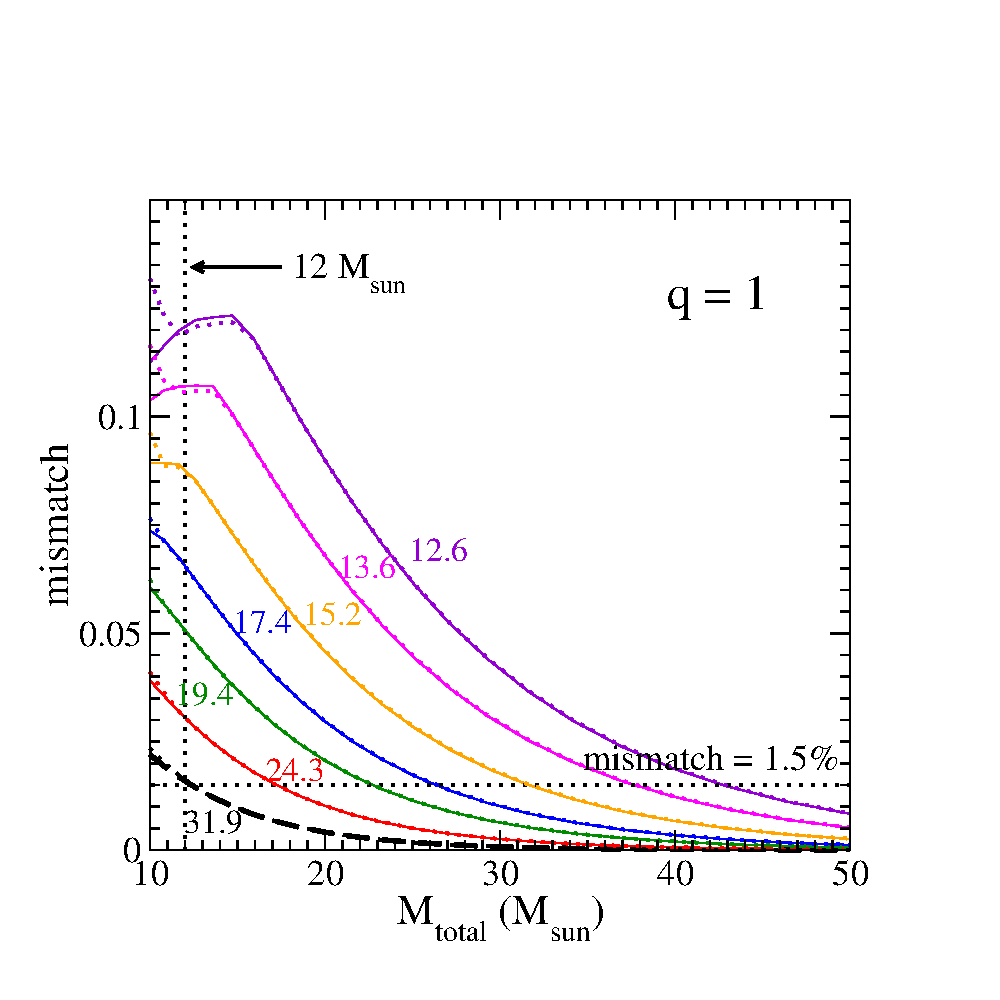
\includegraphics[width=0.55\columnwidth]{figures/nrhybbank/maxmismatchVSmass_q1.pdf}
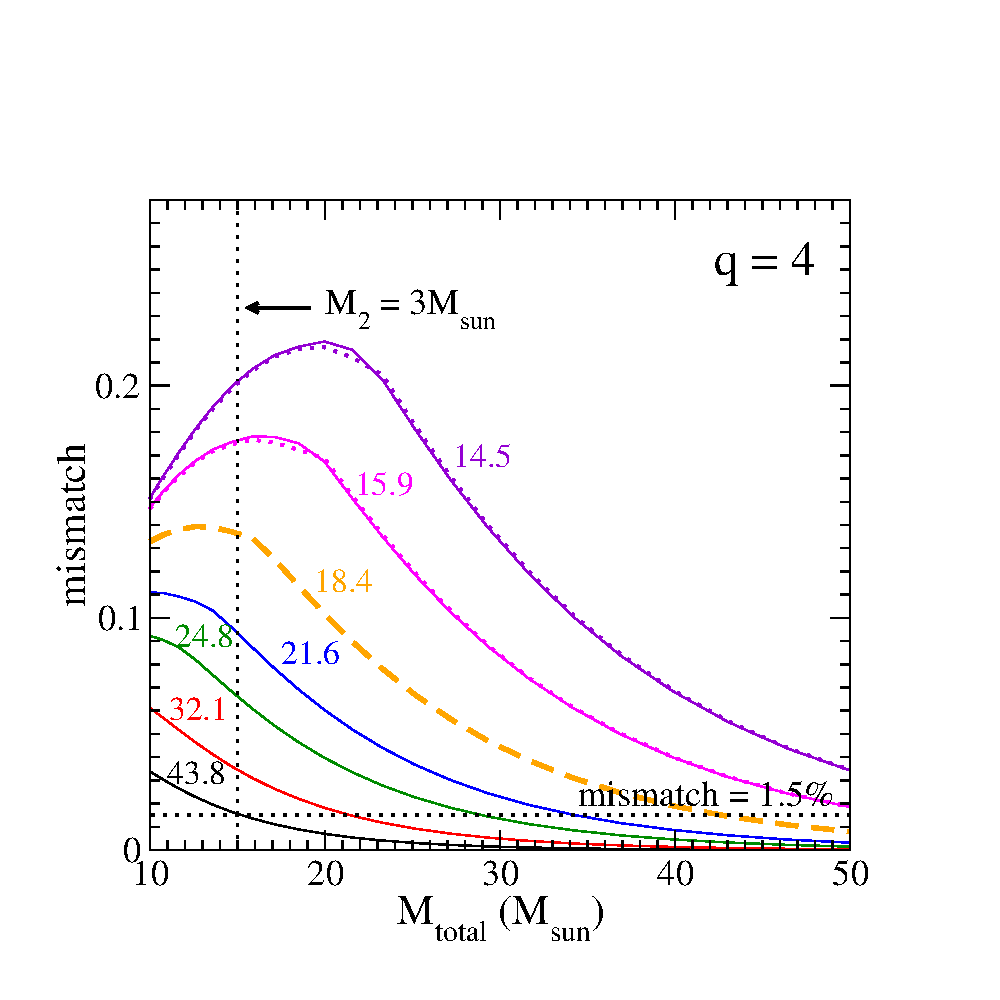
\includegraphics[width=0.55\columnwidth]{figures/nrhybbank/maxmismatchVSmass_q4.pdf}
% \end{center}
\begin{center}
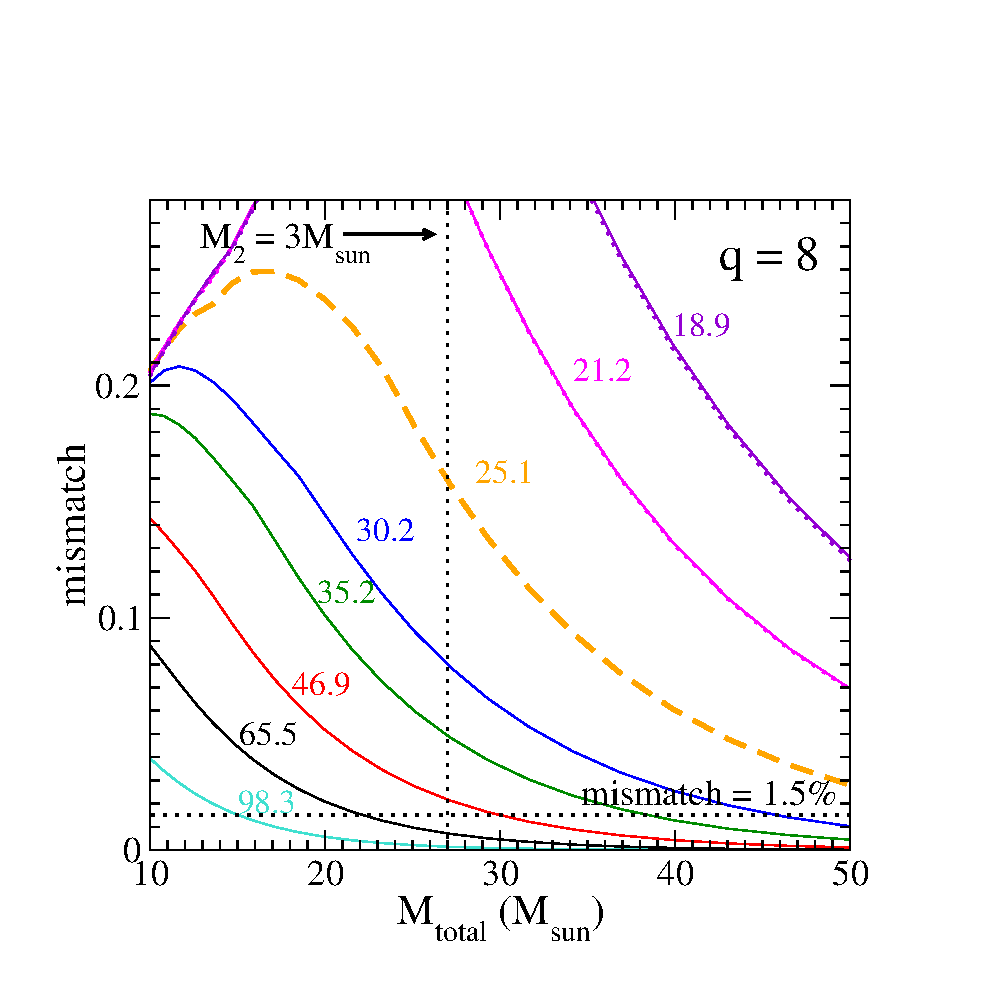
\includegraphics[width=0.6\columnwidth]{figures/nrhybbank/maxmismatchVSmass_q8.pdf}
\end{center}
\caption{\label{fig:maxmismatchVSmass} The maximum mismatch between
  different PN approximants for hybrid waveforms plotted against the
  total mass for at different matching frequencies ($M\omega_m$). The
  dotted lines indicate a mismatch of 1.5\% and a lower total mass
  limit, 12$M_\odot$ for $q=1$, and $M_2 = 3M_\odot$ for $q =
  4,8$. The thick dashed lines indicate the currently possible  
  matching frequency for hybrids based on the length of NR
  waveforms. The numbers next to each line indicate the number of
  orbits before merger where the PN and NR (or EOB) waveforms were 
  stitched together.} 
% \end{center}
\end{figure*}

\begin{figure*}
\begin{center}
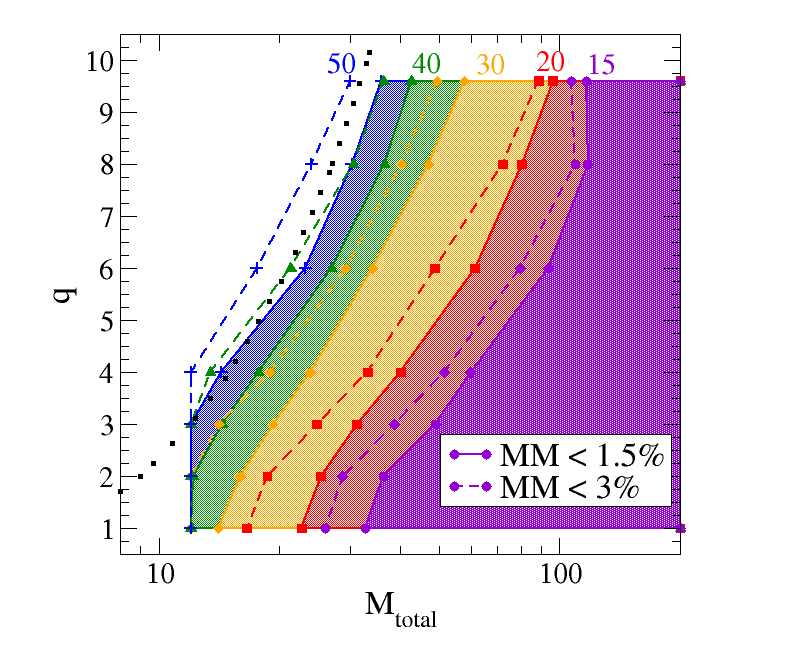
\includegraphics[width=0.7\columnwidth]{figures/nrhybbank/NRorbits2merger_cropped.png}
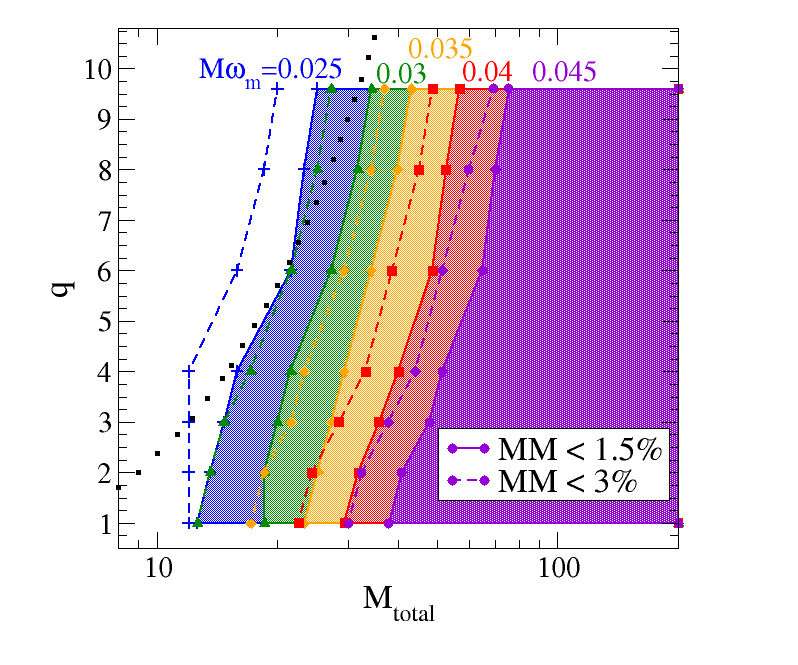
\includegraphics[width=0.7\columnwidth]{figures/nrhybbank/NRomega_cropped.png}
\caption{\label{fig:NRorbits2merger} This plot shows the lower mass limit
  of a template bank constructed with hybrid waveforms in terms of the
number of NR orbits (left panel) and initial gravitational wave
frequency (right panel) needed to have a PN error below $1.5\%$ (solid
curves) or $3\%$ (dashed curves). The dotted line indicates the
lower total mass limit when one component mass is $3M_\odot$.}
\end{center}
\end{figure*}

Having the set of required mass-ratios ${\cal S}_q$ determined, 
we need to decide on the length requirements for the NR simulations,
in order to control the PN hybridization error.  
For a series of matching frequencies, we construct
NR-PN hybrids with Taylor\{T1,T2,T3,T4\} inspirals, and compute their
pairwise mismatch as a function of total mass. The maximum of
these mismatches serves a conservative bound on the PN-hybridization 
error for that hybrid (c.f. Eq.~(\ref{eq:GammaHybfinal})).
Fig.~\ref{fig:maxmismatchVSmass} shows the results of this calculation.
Each panel of
Fig.~\ref{fig:maxmismatchVSmass} focuses on one mass-ratio. Within
each panel, each line represents one matching-frequency, with lines
moving down toward earlier hybridization with smaller mismatches.
Because the hybridization frequency is not particularly intuitive, the
lines are labeled by the number of orbits of the NR portion of the
hybrid-waveform. For a short number of orbits this calculation is
indeed done with NR waveforms, whereas for large number of orbits, we
substitute EOBNRv2 waveforms. The dashed lines represent the earliest
one can match a NR+PN hybrid given the currently available NR
waveforms, and are the same as the $q = 1,4, \text{ and } 8$ lines in
Fig~\ref{fig:Current-NR-PN-Errors}. The solid curves show the results
using EOB hybrids, while the dotted curves (just barely visible) show
the results with NR hybrids. They are virtually identical, which is a
confirmation that EOB hybrids can act as a good proxy for NR
hybrids in this case. The horizontal dotted line
indicates a mismatch of 1.5\%, while the vertical dotted line shows a
lower mass limit for each mass ratio: $12M_\odot$ for $q=1$, which is
the point at which one can construct a template bank with only PN
inspirals, $15M_\odot$ for $q = 4$, and $27M_\odot$ for $q =8$, which
are the lower mass limits if both component masses are $\geq 3M_\odot$. 

Fig.~\ref{fig:NRorbits2merger} presents the information obtained in
the previous paragraph in a different way.  Given NR-PN hybrids with
$N$ orbits of NR, the shaded areas in the left panel of Fig.~\ref{fig:NRorbits2merger}
indicate the region of parameter space for which such hybrids have
hybridization errors smaller than $1.5\%$.  As before, we see that for
high masses, comparatively few NR orbits are sufficient (e.g. the
purple $N=15$ region), whereas lower total masses require increasingly
more NR orbits. The dashed lines indicate the region of parameter
space with hybrid error below $3\%$. The black dotted line designates
the point where one component mass is greater than $3M_\odot$, which
is a reasonable lower mass limit for a physical black hole. The right
panel shows this same analysis instead with initial GW frequency
indicated by the solid and dashed lines. Thus, for the region of
parameter space we're interested in, no more than $\sim 
50$ NR orbits, or an initial GW frequency of $M\omega = 0.025$ would
be necessary to construct a detection bank with  hybrid mismatches
below $1.5\%$.  




%\FloatBarrier
\section{Conclusions}\label{s1:conclusions}

The upgrades currently being installed to increase the sensitivity of the
ground based interferometric gravitational-wave detectors LIGO and
Virgo~\cite{Harry:2010zz,aVIRGO} are scheduled to complete within the next
two years. The second generation detectors will have a factor of $10$ better 
sensitivity across the sensitive frequency band, with the lower frequency
limit being pushed from $40$Hz down to $\sim 10$Hz. 
They will be able to detect GWs from stellar-mass BBHs up to distances of a few
Gpc, with the expected frequency of detection between 
$0.4 - 1000\, yr^{-1}$~\cite{LSCCBCRates2010}.

Gravitational-wave detection searches for BBHs operate by matched-filtering
the detector data against a bank of modeled waveform 
templates~\cite{Babak:2012zx,Sathyaprakash:1991mt, SathyaMetric2PN,
OwenTemplateSpacing,BabaketalBankPlacement,SathyaBankPlacementTauN,
Cokelaer:2007kx}.
Early LIGO-Virgo searches employed PN waveform template banks
that spanned only the inspiral phase of the
coalescence~\cite{Colaboration:2011nz,Abadie:2010yb,Abbott:2009qj,
Abbott:2009tt,Messaritaki:2005wv}.
Recent work has shown that a similar bank of PN templates would be
effectual for the advanced detectors, to detect non-spinning BBHs with 
$m_1 + m_2 \lesssim 12M_\odot$~\cite{Brown:2012nn,CompTemplates2009}.
Searches from the observation period between $2005-07$ and $2009-10$ 
employed templates that also included the late-inspiral, merger and 
ringdown phases of binary coalescence~\cite{Abadie:2011kd,Aasi:2012rja}. 

Recent advancements in Numerical Relativity have led to high-accuracy 
simulations of the late-inspiral and mergers of BBHs. The multi-domain SpEC
code~\cite{spec} has been used to perform simulations for non-spinning 
binaries with mass-ratios
$q=1,2,3,4,6,8$~\cite{Buchman:2012dw,Mroue:2012kv,Mroue:2013xna}. 
Owing to their high computational complexity, the length of these
simulations varies between $15-33$ orbits. Accurate modeling of the
late-inspiral and merger phases is important for stellar mass BBHs,
as they merge at frequencies that the advanced detectors would be 
sensitive to~\cite{Brown:2012nn}. Analytic models, like those within the 
Effective-One-Body formalism, have been calibrated to the NR simulations 
to increase their accuracy during these 
phases~\cite{EOBOriginalBuonannoDamour,EOBNRdevel01,BuonannoEOBv2Main,
Taracchini:2012ig}. Other independent models have also been developed 
using information from NR simulations and their hybrids~\cite{NRAR:home,
Ajith:2007qp,Santamaria:2010yb,Huerta:2012zy}. An alternate derived 
prescription is that of NR+PN hybrid waveforms, that
are constructed by joining long PN early-inspirals and late-inspiral-merger
simulations from NR~\cite{Boyle:2011dy,MacDonald:2011ne,MacDonald:2012mp,
Ohme:2011zm,Hannam:2010ky}. 


NR has long sought to contribute template banks for gravitational-wave
searches. Due to the restrictions on the length and number of NR waveforms,
this has been conventionally pursued by calibrating intermediary
waveform models, and
using those for search templates. In this chapter, we explore the alternative
of using NR waveforms and their hybrids directly in template banks.
We demonstrate the feasibility of this idea for non-spinning binaries,
and extending it to spinning binaries would be the subject of a future
work. We find that with only six non-spinning NR simulations, we can 
cover down to $m_{1,2}\gtrsim 12M_\odot$. We show that with
$26$ additional NR simulations, we can complete the non-spinning template
banks down to $M\simeq 12M_\odot$, below which existing PN waveforms 
have been shown to suffice for aLIGO. From template bank accuracy 
requirements, we are able to put a bound on the required length and 
initial GW frequencies for the new simulations. This method can therefore
be used to lay down the parameters for future simulations. 
%The ability to use hybrid waveforms
%within the software infracture of the LIGO-Virgo collaboration has been 
%demonstrated in the NINJA-2 collaboration~\cite{NINJA2:2013inPrep}. The
%template banks we present here can be directly used in aLIGO searches. 

% We propose the use of the NR waveforms themselves, or hybrids constructed
% out of them, in template banks for aLIGO GW searches. We demonstrate this 
% for the case of non-spinning BBHs, and aim to extend to spinning binaries 
% in future work. There are two benefits of using hybrid waveforms in 
% template banks. First, the intrinsic model errors in hybrid waveforms 
% arise out of the yet-unknown higher-order PN terms. These errors can be
% (conservatively) put a bound on~\cite{MacDonald:2011ne,MacDonald:2012mp}, 
% and we show that they can and should be taken into account when 
% constructing banks for stellar mass BBHs. Complete IMR waveform models
% are based on resummed or phenomenological extensions of PN calculations.
% Their free parameters are fitted to ensure the model agrees with NR 
% simulations that span a few tens of orbits before merger.
% However, their intrinsic errors in the late-inspiral regime, where the 
% PN theory begins to be inaccurate, are difficult to precisely quantify;
% especially for binary masses and spins to which the models are 
% interpolated or extrapolated to. Bounding of model errors in hybrids is
% useful for developing conservatively effectual banks. We expect this
% to be an even bigger advantage for template banks for spinning BBHs.
% Second, we are able to predict the simulations that would be required
% to complete the hybrid bank at lower masses, down to $M\sim 12M_\odot$.
% This is useful in choosing parameters for future NR simulations, which
% can be directly applied to GW searches.

First, we construct a bank for using pure-NR waveforms as templates, 
using a stochastic algorithm similar to Ref.~\cite{Harry:2009ea,
Ajith:2012mn,Manca:2009xw}. The filter templates are constrained to 
mass-ratios for which we have NR simulations available, i.e. 
$q=1,2,3,4,6,8$. 
We assume that the simulations available to us are $\geq 20$ orbits in
length. To test the bank, we simulate a population of $100,000$ BBH 
signals and filter them through the bank. The signals and templates 
are both modeled with the EOBNRv2 model~\cite{BuonannoEOBv2Main}. We 
demonstrate that this bank is indeed effectual and recovers 
$\geq 97\%$ of the optimal SNR for GWs from BBHs with mass-ratios 
$1\leq q\leq 10$ and chirp-mass 
$\mathcal{M}_c\equiv (m_1+m_2)^{-1/5}(m_1 m_2)^{3/5}$ above $27M_\odot$. 
Fig.~\ref{fig:bank001_01_match} shows this fraction at different 
simulated points over the binary mass space. With an additional 
simulation for $q=9.2$, we are able to extend the coverage to higher
mass-ratios. We show that a bank viable for NR waveform templates for
$q=1,2,3,4,6,9.2$, would recover $\geq 97\%$ of the optimal SNR
for BBHs with $10\leq q\leq 11$. The SNR recovery fraction from
such a bank is shown in Fig.~\ref{fig:bank006_01_match}.


Second, we construct effectual banks for currently available
NR-PN hybrid waveform templates. We derive a bound on waveform model
errors, which is independent of analytical models and can be used
to independently assess the errors of such models (see
Sec.~\ref{s1:quantifyingerrors} for details). This allows us to estimate
the hybrid waveform mismatches due to PN error, which are negligible
at high masses, and become significant at lower binary masses. We
take their contribution to the SNR loss into account while 
characterizing template banks. For hybrid banks, we demonstrate and 
compare two independent algorithms of template bank construction. 
First, we stochastically
place a bank grid, as for the purely-NR template bank. Second, we lay down
independent sub-banks for each mass-ratio, with a fixed overlap between
neighboring templates, and take their union as the final bank. 
To test these banks, we simulate a population of $100,000$ BBH signals
and filter them through each. We simulate the GW signals and the 
templates using the recently developed EOBNRv2 model~\cite{BuonannoEOBv2Main}. 
The fraction of the optimal SNR recovered by the two banks, before and after
accounting for the hybrid errors, are shown in the left and right panels 
of Fig.~\ref{fig:Current-hybrids-stochastic-FF} and 
Fig.~\ref{fig:Current-hybrids-FF} (respectively).
We observe that for BBHs with $m_{1,2}\geq 12M_\odot$ hybrid template 
banks will recover $\geq 96.5\%$ of the optimal SNR.  For testing the
robustness of our conclusions, we also test the banks using TaylorT4+NR
hybrid templates. The SNR recovery from a bank of these is shown in
Fig.~\ref{fig:Current-real-hybrids-FF}. We conclude that, 
the currently available NR+PN hybrid waveforms can be used as templates in 
a matched-filtering search for GWs from BBHs with $m_{1,2}\geq 12M_\odot$
and $1\leq q\leq 10$. The number of templates required to provide coverage
over this region was found to be comparable to a bank constructed using 
the second-order post-Newtonian TaylorF2 hexagonal template placement 
method~\cite{SathyaBankPlacementTauN,BabaketalBankPlacement,
SathyaMetric2PN,Cokelaer:2007kx}.
The two algorithms we demonstrate yield grids of $667$ and $627$ templates,
respectively; while the metric based placement method yields a grid of $522$ 
and $736$ templates, for $97\%$ and $98\%$ minimal match, respectively.


At lower mass, the length of the waveform in the sensitive frequency
band of the detectors increases, increasing the resolution of 
the matched-filter. We therefore see regions of undercoverage 
between mass ratios for which we have NR/hybrid templates 
(see, e.g. Fig.~\ref{fig:Current-hybrids-FF} at the left edge).
For $M\lesssim 12M_\odot$, existing PN waveforms were shown to 
be sufficient for aLIGO searches. 
We find the additional simulations that would be needed to extend
the hybrid tempalte bank down to $12M_\odot$. We show that a bank
of hybrids restricted to the $26$ mass-ratios listed in 
Table~\ref{table:fullqlist} would be sufficiently dense at $12M_\odot$.
This demonstrates that the method proposed here can be used 
to decide which NR simulations should be prioritized for the purpose
of the GW detection problem.
By filtering a population of $100,000$ BBH signals
through this bank, we show that the SNR loss due to its discreteness
stays below $2\%$ over the entire relevant range of masses.
The fraction of optimal SNR recovered is shown in 
Fig.~\ref{fig:templatebank_halfMassRatios}. Constraining the 
detection rate loss below $10\%$ requires that detection template 
banks recover more than $96.5\%$ of the optimal SNR. Therefore
our bank would need hybrids with hybridization mismatches below 
$1.5\%$. From this accuracy requirement, we obtain the length
requirement for all the $26$ simulations. This is depicted in the 
left panel of Fig.~\ref{fig:NRorbits2merger}, where we show the region
of the mass space that can be covered with hybrids, as the length of 
their NR portion varies. We find that for $1\leq q\leq 10$  the 
new simulations should be about $50$ orbits in length. In the right 
panel of Fig.~\ref{fig:NRorbits2merger} we show the corresponding
initial GW frequencies. The requirement of $\sim 50$ orbit long NR
simulations is ambitious, but certainly feasible with the current BBH 
simulation technology~\cite{BelaLongSimulation}.

In summary, we refer to the right panel of
Fig.~\ref{fig:templatebank_halfMassRatios}.
The region above the dashed (red) line and above the solid (blue) line can
be covered with a bank of purely-NR waveforms currently available. The region
above the dashed (red) and the dash-dotted (black) line can be covered with
the same simulations hybridized to long PN inspirals. With an additional set
of NR simulations summarized in Table~\ref{table:fullqlist}, the coverage
of the bank can be extended down to the magenta (solid) line in the lower
left corner of the figure. Thus between hybrids and PN waveforms, 
we can cover the entire non-spinning BBH space. The ability to use hybrid
waveforms within the software infrastructure of the LIGO-Virgo collaboration 
has been demonstrated in the NINJA-2 collaboration~\cite{NINJA2:2013inPrep}.
The template banks we present here can be directly used in aLIGO searches. 
This work will be most useful when extended to aligned spin and 
precessing binaries~\cite{Boyle:2013nka,Schmidt:2012rh}, which is the
subject of a future work.

The detector noise power is modeled using the zero-detuning high-power 
noise curve for Advanced LIGO~\cite{aLIGONoiseCurve}.
The construction of our template banks is sensitive to the breadth
of the frequency range that the detector would be 
sensitive to. The noise curve we use is the broad-band final design 
sensitivity estimate. For lower sensitivities
at the low/high frequencies, our results would become more conservative, 
i.e. the template banks would over-cover (and not under-cover).

We finally note that in this chapter we have only considered the
dominant $(2,2)$ mode of the spherical decomposition of the 
gravitational waveform. For high mass-ratios and high binary masses,
other modes would also become important, both for spinning as well
as non-spinning black hole binaries~\cite{Pekowsky:2012sr,
Brown:2012nn,Capano:2013inPrep}.
Thus, in future work, it would be relevant to examine the
sub-dominant modes of the gravitational waves. Lastly, though we have
looked at the feasibility of using this template bank for Advanced
LIGO as a single detector, this instrument will be part of a network
of detectors, which comes with increased sensitivity and sky
localization. For this reason, in subsequent studies it would be
useful to consider a network of detectors.


\Chapter{NINJA-2: Detecting gravitational waveforms modelled
using numerical binary black hole simulations}
\label{ch:ninja2}
The NINJA-1 project was a huge success in bringing the numerical
relativity and gravitational-wave astronomy communities together.  The
project also resulted in several intriguing qualitative results.
However, it only began the process of testing detection and parameter
estimation pipelines against realistic signals.  The follow-up
project, NINJA-2, is ongoing as of the time of writing.  NINJA-2 aims
to remove some of the shortcomings of NINJA-1 and allow quantitative
studies of the behaviors of pipelines in varying regions of signal
parameter space.  Specifically, NINJA-2 addresses issues with both the
waveform submissions and the noise used to construct the data sets.

This chapter describes the contributed waveforms, the studies that
have been done to verify them, and the construction of the first round
of data sets.  The next chapter will present preliminary results from
running the CBC pipelines on the longest and most carefully
constructed of these data sets.

\section{Contributed waveforms}

NINJA-1 had an open policy towards waveforms submission in order to
encourage wide participation.  This meant there were no requirements
on either waveform quality or length.  The lack of quality
requirements allowed for the possibility of unphysical features in the
waveforms.  There were also no requirements to perform the kind of
convergence testing reported in section~\ref{sec:PNNRHybridWaveform},
although such validation is typically done by numerical
relativistists.  The loose requirements limited the conclusions that
could be drawn, for example it makes it difficult to say whether an
injection was missed due to the parameters of the signal or an
unintended feature of the waveform.

The lack of length requirement limited the available mass range to $M
< 36 \msun$ for reasons that can be seen in
figure~\ref{fig:StildesAndInitialPSD}.   Had the waveform in that plot
not had a post-Newtonian component, the NR component to the right of
the triangles would have had to be placed below 40 Hz in order to
prevent turning on in-band.  This mass range limited the tests that
could be done, for example it entirely excludes the standard CBC
low-mass pipeline.

To address these issues NINJA-2 specifies the following minimal
requirements~\cite{ninja2-wiki}.  The raw numerical simulation should
include at least five orbits of usable data before merger (i.e., not
counting bursts of junk radiation or other significant noise).  Given
the computation cost of extending the NR waveforms, we instead require
stitching to a post-Newtonian inspiral approximant, which should be
performed at a GW frequency of $M\omega ≤ 0.075$, where $M\omega$ is
the frequency of the $(l = 2, m = \pm 2)$ harmonic. The full waveform
should be long enough to be entirely within the sensitivity bands of
LIGO and Virgo down to $10 \msun$ with a lower cutoff frequency of 10
Hz, which corresponds to a starting GW frequency of $M\omega = 0.003$.
The numerical-waveform (before any hybridization) amplitude should be
accurate to within 5\%, and the phase (as a function of GW frequency)
should have an accumulated uncertainty over the entire inspiral,
merger and ringdown, of no more than 0.5 radian. The PN approximants
used for hybridization should ideally use the highest PN orders
available, both in phase and amplitude.  

These minimal accuracy requirements are motivated by the results of
the Samurai project~\cite{Hannam:2009hh}, and studies performed in
preparation for the NR-AR collaboration project~\cite{ninja-wiki}.
The question of how many NR cycles are needed in order to produce a
robust waveform is an area of current research. \Note{cite Ilana}.

The NINJA-2 project encourages although does not require the addition
of higher-order modes.  We chose to restrict attention to non-spinning
waveforms and waveforms with spins aligned or anti-aligned with the
orbital angular momentum.  There are sufficient open questions
regarding these restricted cases to make this analysis interesting,
without adding the additional complications on both the NR and data
analysis sides associated with precession. 

A total of 60 waveforms from 8 groups were contributed, these are
summarized in tables ~\ref{tab:ninja2_bam}, \ref{tab:ninja2_fau},
\ref{tab:ninja2_gatech}, \ref{tab:ninja2_lean},
\ref{tab:ninja2_llama}, \ref{tab:ninja2_rit}, \ref{tab:ninja2_spec},
\ref{tab:ninja2_uiuc} and a map of the parameter values is shown in
figure~\ref{f:ninja2_param_map}.

\begin{table}
\begin{center}
\begin{tabular}{|l|r|r|r|l|c|}
\hline
Run & $q$ & Spin1${}_z$ & Spin2${}_z$ & pN Approx. & Refs \\
\hline
BAM\_D10spp85\_80.T4.hyb.n2 & 1 & 0.85 & 0.85 & TaylorT4 & \cite{Hannam:2007wf,Brugmann:2008zz} \\
BAM\_D10spp85\_80.T1.hyb.n2 & 1 & 0.85 & 0.85 & TaylorT1 & \cite{Hannam:2007wf,Brugmann:2008zz} \\
BAM\_D125smm50Nep\_80.T1.hyb.n2 & 1 & -0.50 & -0.50 & TaylorT1 & \cite{Hannam:2007wf,Brugmann:2008zz} \\
BAM\_D125smm50Nep\_80.T4.hyb.n2 & 1 & -0.50 & -0.50 & TaylorT4 & \cite{Hannam:2007wf,Brugmann:2008zz} \\
BAM\_D13smm75Nep\_96.T4.hyb.n2 & 1 & -0.75 & -0.75 & TaylorT4 & \cite{Hannam:2007wf,Brugmann:2008zz} \\
BAM\_D13smm75Nep\_96.T1.hyb.n2 & 1 & -0.75 & -0.75 & TaylorT1 & \cite{Hannam:2007wf,Brugmann:2008zz} \\
BAM\_D13smm85Nep\_88.T4.hyb.n2 & 1 & -0.85 & -0.85 & TaylorT4 & \cite{Hannam:2007wf,Brugmann:2008zz} \\
BAM\_D13smm85Nep\_88.T1.hyb.n2 & 1 & -0.85 & -0.85 & TaylorT1 & \cite{Hannam:2007wf,Brugmann:2008zz} \\
BAM\_D11spp50\_96.T4.hyb.n2 & 1 & 0.50 & 0.50 & TaylorT4 & \cite{Hannam:2007wf,Brugmann:2008zz} \\
BAM\_D11spp50\_96.T1.hyb.n2 & 1 & 0.50 & 0.50 & TaylorT1 & \cite{Hannam:2007wf,Brugmann:2008zz} \\
BAM\_D10spp75\_80.T1.hyb.n2 & 1 & 0.75 & 0.75 & TaylorT1 & \cite{Hannam:2007wf,Brugmann:2008zz} \\
BAM\_D10spp75\_80.T4.hyb.n2 & 1 & 0.75 & 0.75 & TaylorT4 & \cite{Hannam:2007wf,Brugmann:2008zz} \\
BAM\_D12smm25Nep\_80.T4.hyb.n2 & 1 & -0.25 & -0.25 & TaylorT4 & \cite{Hannam:2007wf,Brugmann:2008zz} \\
BAM\_D12smm25Nep\_80.T1.hyb.n2 & 1 & -0.25 & -0.25 & TaylorT1 & \cite{Hannam:2007wf,Brugmann:2008zz} \\
BAM\_EP\_um4\_D10-n96.T4.hyb.n2 & 4 & 0.00 & 0.00 & TaylorT4 & \cite{Hannam:2007wf,Brugmann:2008zz} \\
BAM\_EP\_um4\_D10-n96.T1.hyb.n2 & 4 & 0.00 & 0.00 & TaylorT1 & \cite{Hannam:2007wf,Brugmann:2008zz} \\
BAM\_um3\_88.T4.hyb.n2 & 3 & 0.00 & 0.00 & TaylorT4 & \cite{Hannam:2007wf,Brugmann:2008zz} \\
BAM\_um3\_88.T1.hyb.n2 & 3 & 0.00 & 0.00 & TaylorT1 & \cite{Hannam:2007wf,Brugmann:2008zz} \\
BAM\_um2\_88.T1.hyb.n2 & 2 & 0.00 & 0.00 & TaylorT1 & \cite{Hannam:2007wf,Brugmann:2008zz} \\
BAM\_um2\_88.T4.hyb.n2 & 2 & 0.00 & 0.00 & TaylorT4 & \cite{Hannam:2007wf,Brugmann:2008zz} \\
BAM\_R6\_PN\_80.T1.hyb.n2 & 1 & 0.00 & 0.00 & TaylorT1 & \cite{Hannam:2007wf,Brugmann:2008zz} \\
BAM\_R6\_PN\_80.T4.hyb.n2 & 1 & 0.00 & 0.00 & TaylorT4 & \cite{Hannam:2007wf,Brugmann:2008zz} \\
BAM\_D12spp25\_96.T4.hyb.n2 & 1 & 0.25 & 0.25 & TaylorT4 & \cite{Hannam:2007wf,Brugmann:2008zz} \\
BAM\_D12spp25\_96.T1.hyb.n2 & 1 & 0.25 & 0.25 & TaylorT1 & \cite{Hannam:2007wf,Brugmann:2008zz} \\
BAM\_q2a0a025\_T\_96\_344.T1.hyb.n2.bbh & 2 & 0.25 & 0.00 & {} & \cite{,Brugmann:2008zz} \\
BAM\_q2a0a025\_T\_96\_344.T4.hyb.n2.bbh & 2 & 0.25 & 0.00 & {} & \cite{,Brugmann:2008zz} \\
\hline
\end{tabular}
\end{center}
\caption[BAM submissions to NINJA-2]{
\label{tab:ninja2_bam}
BAM submissions to NINJA-2}
\end{table}

\begin{table}
\begin{center}
\begin{tabular}{|l|r|r|r|l|c|}
\hline
Run & $q$ & Spin1${}_z$ & Spin2${}_z$ & pN Approx. & Refs \\
\hline
BAM\_hybrid\_om0.025etmq3S0.4- & 3 & 0.40 & 0.60 & TaylorT4 & \cite{none,???} \\
0\_0\_S0.6\_0\_0\_72 &  &  &  &  &  \\
\hline
\end{tabular}
\end{center}
\caption[FAU submissions to NINJA-2]{
\label{tab:ninja2_fau}
FAU submissions to NINJA-2}
\end{table}

\begin{table}
\begin{center}
\begin{tabular}{|l|r|r|r|l|c|}
\hline
Run & $q$ & Spin1${}_z$ & Spin2${}_z$ & pN Approx. & Refs \\
\hline
MayaKranc\_D12\_a0.00\_m129\_nj & 1 & 0.00 & 0.00 & TaylorT4 & \cite{,} \\
MayaKranc\_D10\_a0.90\_m129\_nj & 1 & 0.90 & 0.90 & TaylorT4 & \cite{,} \\
MayaKranc\_D10\_a0.20\_m77\_nj & 1 & 0.20 & 0.20 & TaylorT4 & \cite{,} \\
MayaKranc\_D10\_a0.60\_m77\_nj & 1 & 0.60 & 0.60 & TaylorT4 & \cite{,} \\
MayaKranc\_D12\_a0.60\_m103\_nj & 1 & 0.60 & 0.60 & TaylorT4 & \cite{,} \\
MayaKranc\_Sp02py0935th90\_gr & 1 & 0.80 & 0.00 & TaylorT4 & \cite{,} \\
MayaKranc\_D12\_a0.80\_m103\_nj & 1 & 0.80 & 0.80 & TaylorT4 & \cite{,} \\
MayaKranc\_D12\_a0.00\_q2\_m90\_nj & 2 & 0.00 & 0.00 & TaylorT4 & \cite{,} \\
MayaKranc\_D11\_a0.20\_q2\_m90\_nj & 2 & 0.02 & 0.09 & TaylorT4 & \cite{,} \\
MayaKranc\_D10\_a0.40\_m90\_nj & 1 & 0.40 & 0.40 & TaylorT4 & \cite{,} \\
MayaKranc\_D10\_a0.80\_m90\_nj & 1 & 0.80 & 0.80 & TaylorT4 & \cite{,} \\
MayaKranc\_D12\_a0.40\_m103\_nj & 1 & 0.40 & 0.40 & TaylorT4 & \cite{,} \\
MayaKranc\_D12\_a0.20\_m103\_nj & 1 & 0.20 & 0.20 & TaylorT4 & \cite{,} \\
\hline
\end{tabular}
\end{center}
\caption[GATech submissions to NINJA-2]{
\label{tab:ninja2_gatech}
GATech submissions to NINJA-2}
\end{table}

\begin{table}
\begin{center}
\begin{tabular}{|l|r|r|r|l|c|}
\hline
Run & $q$ & Spin1${}_z$ & Spin2${}_z$ & pN Approx. & Refs \\
\hline
dq4 & 4 & 0.00 & 0.00 & TaylorT1 & \cite{,Sperhake:2006cy} \\
\hline
\end{tabular}
\end{center}
\caption[LEAN submissions to NINJA-2]{
\label{tab:ninja2_lean}
LEAN submissions to NINJA-2}
\end{table}

\begin{table}
\begin{center}
\begin{tabular}{|l|r|r|r|l|c|}
\hline
Run & $q$ & Spin1${}_z$ & Spin2${}_z$ & pN Approx. & Refs \\
\hline
Llama\_d550-h64-Hybrid & 1 & 0.00 & 0.00 & 3.5pNTaylorF2 & \cite{Reisswig:2009rx,Reisswig:2009rx} \\
Llama\_d4d4-q1--D10-h64-r250.T4.hybrid & 1 & -0.40 & -0.40 & TaylorT4 & \cite{Pollney:2010hs,Pollney:2009yz,} \\
Llama\_d4d4-q1--D10-h64-r250.T1.hybrid & 1 & -0.40 & -0.40 & TaylorT1 & \cite{Pollney:2010hs,Pollney:2009yz,} \\
Llama\_u4u4-q1--D8-h64-r250.T1.hybrid & 1 & 0.40 & 0.40 & TaylorT1 & \cite{Pollney:2010hs,Pollney:2009yz,} \\
Llama\_u4u4-q1--D8-h64-r250.T4.hybrid & 1 & 0.40 & 0.40 & TaylorT4 & \cite{Pollney:2010hs,Pollney:2009yz,} \\
Llama\_d5q2-h016-Hybrid & 2 & 0.00 & 0.00 & 3.5pNTaylorF2 & \cite{,Reisswig:2009rx} \\
Llama\_u2u2-q1--D8-h64-r250.T1.hybrid & 1 & 0.20 & 0.20 & TaylorT1 & \cite{Pollney:2010hs,Pollney:2009yz,} \\
Llama\_u2u2-q1--D8-h64-r250.T4.hybrid & 1 & 0.20 & 0.20 & TaylorT4 & \cite{Pollney:2010hs,Pollney:2009yz,} \\
Llama\_d2d2-q1--D10-h64-r250.T1.hybrid & 1 & -0.20 & -0.20 & TaylorT1 & \cite{Pollney:2010hs,Pollney:2009yz,} \\
Llama\_d2d2-q1--D10-h64-r250.T4.hybrid & 1 & -0.20 & -0.20 & TaylorT4 & \cite{Pollney:2010hs,Pollney:2009yz,} \\
\hline
\end{tabular}
\end{center}
\caption[Llama submissions to NINJA-2]{
\label{tab:ninja2_llama}
Llama submissions to NINJA-2}
\end{table}

\begin{table}
\begin{center}
\begin{tabular}{|l|r|r|r|l|c|}
\hline
Run & $q$ & Spin1${}_z$ & Spin2${}_z$ & pN Approx. & Refs \\
\hline
LazEV\_D8.4\_10to1\_nj\_hybrid & 10 & 0.00 & 0.00 & TaylorT4 & \cite{Campanelli:2005dd} \\
\hline
\end{tabular}
\end{center}
\caption[RIT submissions to NINJA-2]{
\label{tab:ninja2_rit}
RIT submissions to NINJA-2}
\end{table}

\begin{table}
\begin{center}
\begin{tabular}{|l|r|r|r|l|c|}
\hline
Run & $q$ & Spin1${}_z$ & Spin2${}_z$ & pN Approx. & Refs \\
\hline
SpEC\_q6s0 & 6 & 0.00 & 0.00 & TaylorT1 & \cite{SpECWebsite} \\
SpEC\_q4s0 & 4 & 0.00 & 0.00 & TaylorT2 & \cite{SpECWebsite} \\
SpEC\_EqualMassAntiAlignedSpins & 1 & -0.44 & -0.44 & NA & \cite{chu-2009,SpECWebsite} \\
SpEC\_q1s-0.95 & 1 & -0.95 & -0.95 & TaylorT1 & \cite{SpECWebsite} \\
SpEC\_q2s0 & 2 & 0.00 & 0.00 & TaylorT2 & \cite{SpECWebsite} \\
SpEC\_EqualMassAlignedSpins & 1 & 0.44 & 0.44 & NA & \cite{chu-2009,SpECWebsite} \\
SpEC\_q3s0 & 3 & 0.00 & 0.00 & TaylorT2 & \cite{SpECWebsite} \\
SpEC\_EqualMassNonspinning & 1 & 0.00 & 0.00 & TaylorT4 & \cite{Scheel:2008rj,SpECWebsite} \\
\hline
\end{tabular}
\end{center}
\caption[SpEC submissions to NINJA-2]{
\label{tab:ninja2_spec}
SpEC submissions to NINJA-2}
\end{table}

\begin{table}
\begin{center}
\begin{tabular}{|l|r|r|r|l|c|}
\hline
Run & $q$ & Spin1${}_z$ & Spin2${}_z$ & pN Approx. & Refs \\
\hline
UIUC\_spin\_-0.25\_om0.0528\_22-HYBRID & 1 & -0.25 & -0.25 & NA & \cite{none} \\
UIUC\_spin\_0.85\_om0.0536\_22-HYBRID & 1 & 0.85 & 0.85 & NA & \cite{none} \\
\hline
\end{tabular}
\end{center}
\caption[UIUC submissions to NINJA-2]{
\label{tab:ninja2_uiuc}
UIUC submissions to NINJA-2}
\end{table}


\begin{figure}
  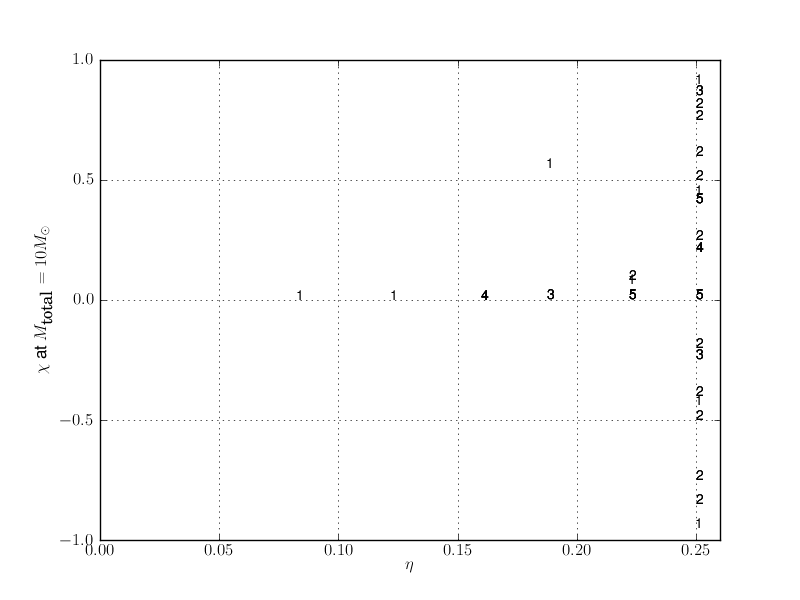
\includegraphics[width=\linewidth]{figures/ninja2/ninja2_cat.png}
  \caption[Parameters of the NINJA-2 submissions]{
  \label{f:ninja2_param_map}
Parameters of the NINJA-2 hybrid waveform submissions showing the
symmetric mass ratio $\eta=m_1 m_2 /(m_1+m_2)^2$ and dimensionless
spin parameter $\chi=(S_1/m_1 + S_2/m_2)/(m_1+m_2)$ after scaling the
waveforms to a total mass of 10 $\msun$.  The numbers indicate how
many distinct waveforms with the specified parameters were submitted.}
\end{figure}%

\section{Verifying the hybrid waveforms}

Each NR group verified that their waveforms met the minimum NINJA-2
requirements before submission.  Once submitted, a series of checks
were performed in order to validate the waveforms against each other.

In the first stage the post-Newtonian expressions and codes were
compared against each other and the literature.  This required several
iterations, but resulted in a set of codes in various languages that
produce waveforms that all agree in both phase and amplitude. 

\subsection{Time-domain and frequency-domain checks}

In the second stage the complete hybrid waveforms were examined.
We first plotted the last 40 cycles of each waveform -- enough to
include the full NR portion, the hybridization region, and some of the
pN portion -- and looked for any anomalies such as those present in
some of the NINJA-1 waveforms in figure~\ref{fig:NR-Reh22}.  A few such
features were indeed visible, spotting them in this way allowed them
to be corrected.  One example is shown in figure (\Note{show the dq4
waveform before and after, note this was due to a problem integrating
psi4, and discuss this stage a little in the NR section of chapter
3}).

The amplitude of the Fourier transform of the complete waveforms were
also plotted.  This analysis also revealed unphysical features, 
primarily due to hybridization.  An example is shown in
figure~\ref{f:ninja2_freq_hybrids}, which shows a visible ``kink'' in
the waveform at the hybridization frequency, which vanishes after the
waveform was reconstructed.

\begin{figure}
  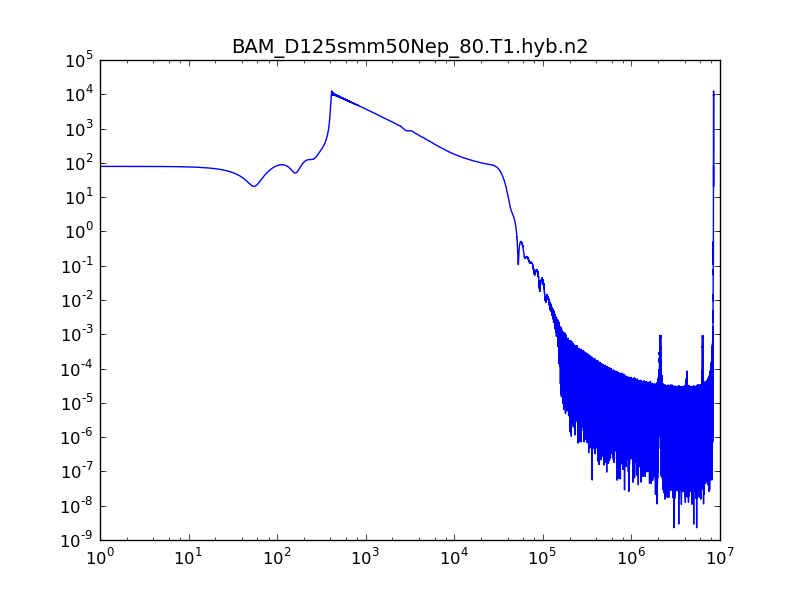
\includegraphics[width=0.5\linewidth]{figures/ninja2/bam_d125smm50nep_80_t1_hyb_n2_amp.png}
  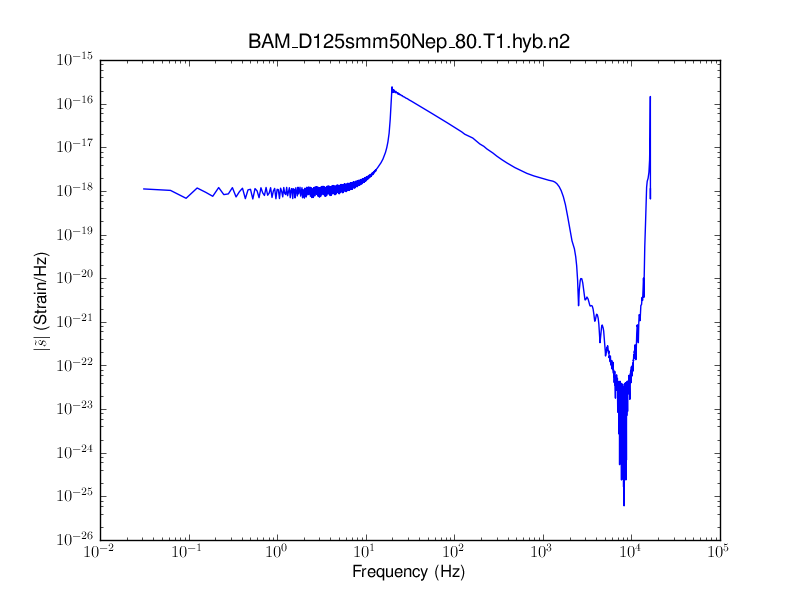
\includegraphics[width=0.5\linewidth]{figures/ninja2/bam_d125smm50nep_80_t1_hyb_n2_amp_v2.png}
  \caption[Frequency-domain hybrid NINJA-2 waveforms]{
  \label{f:ninja2_freq_hybrids}
Fourier amplitude of the (2,2) mode of a sample NINJA-2 hybrid
waveform from the BAM/AEI group.  The waveform has been scaled to 10
$\msun$ and placed 1 Mpc from the detector to give it physical units.
\Note{I need to dig up the old version of the waveform and remake it
with the new code} The waveform on the left is the version
initially submitted, note there is a visible ``kink'' in the waveform
at the hybridization frequency.  The waveform on the right has been
re-hybridized and there is no longer a visible kink.  This feature did
not show up in the time domain view of the waveform.}
\end{figure}%


\subsection{Overlap comparisons}

In tis check the waveforms were compared against each other using
standard data-analysis techniques, in particular the overlap defined
in section~\ref{sec:search_matchfilter}. 

\begin{figure}
  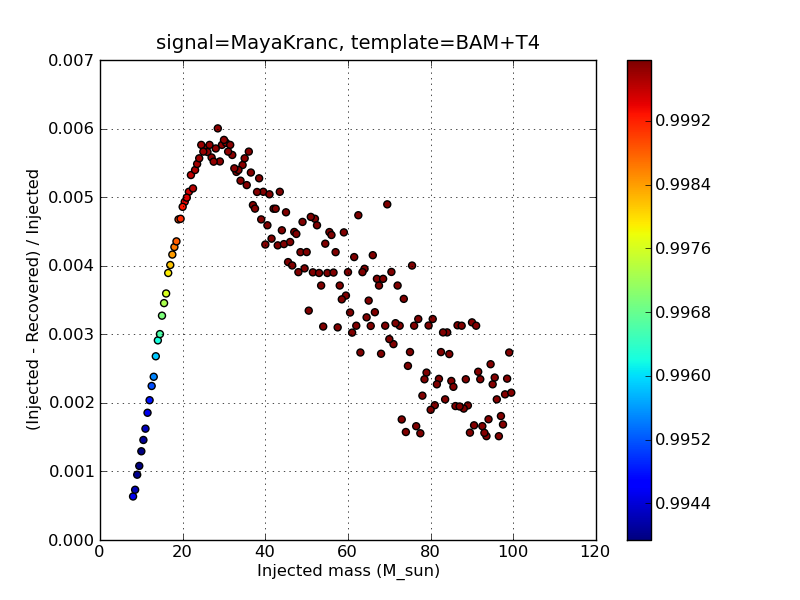
\includegraphics[width=0.5\linewidth]{figures/ninja2/maya_bamt4_max_over_m}
  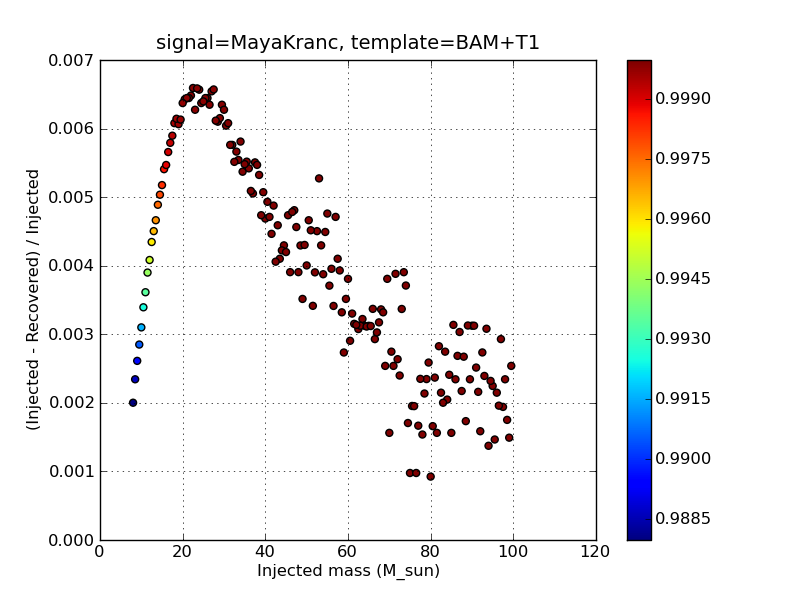
\includegraphics[width=0.5\linewidth]{figures/ninja2/maya_bamt1_max_over_m}
  \caption[Overlaps between NINJA-2 submissions maximized over mass]{
  \label{f:ninja2_max_over_mass_bam}
Overlaps between the equal-mass, non-spinning MayaKranc waveform taken
as the signal, and the equal-mass, non-spinning BAM waveform
hybridized with TaylorT4 (left) and TaylorT1 (right) taken as
templates.  Maximization is done over mass, as well as time and phase.
Note the lower overall overlaps and mass bias at the low-mass end,
where the two pN waveforms dominate the overlap.}
\end{figure}%


\section{Construction of the NINJA-2 data set}

\begin{figure}
  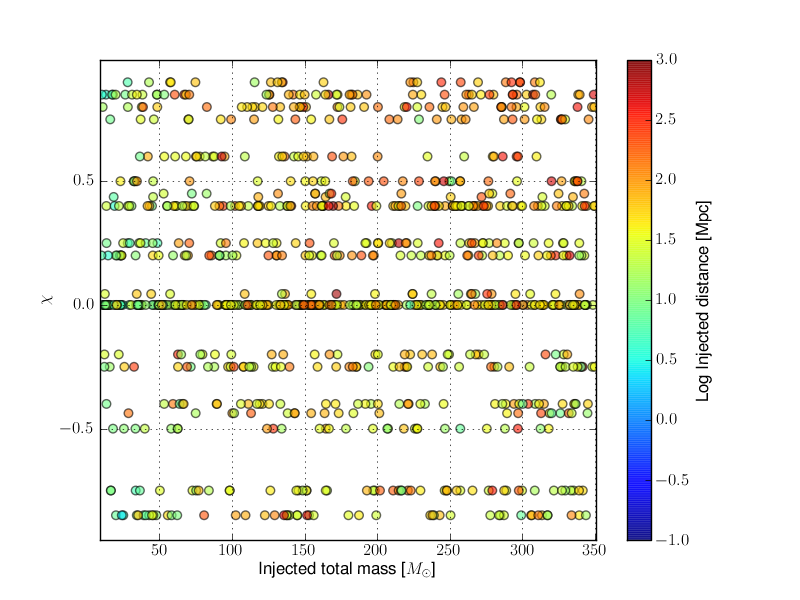
\includegraphics[width=\linewidth]{figures/ninja2/ninja2_dataset.png}
  \caption[Parameters of the NINJA-2 two-month data set]{
  \label{f:ninja2_dataset}
Distribution of mass, spin and distance parameters in the two-month,
Gaussian-noise data set.
}
\end{figure}%



% TODO:
% make tables of submissions
% plot of paramater space in eta, chi scaled to 10 M
% plot of injection set (use chi instead of sum of magnitudes)
% text
% results
% explain move to 16384 (plot showing aliasing)



\Chapter{Modeling of intermediate mass-ratio inspirals: 
Exploring the form of the self-force in the intermediate mass-ratio regime}
\label{ch:insSFIMRI}
%%%%%%%%%%%%%%%%%%%%%%%%%%%%%%%%%%%%%%%%%%%%%%%%%%%%%%%%%%%%%%%%%%%%%%%%%%%%%%%
%%% Describe the inspiral model for IMRIs.
%%%%%%%%%%%%%%%%%%%%%%%%%%%%%%%%%%%%%%%%%%%%%%%%%%%%%%%%%%%%%%%%%%%%%%%%%%%%%%%

\newcommand {\MBH}{{\cal{M}_{\bullet}}}
\newcommand {\Msun}{\ensuremath{M_{\odot}}}
\newcommand {\Mstar}{\ensuremath{M_{\ast}}}
\newcommand {\Nstar}{\ensuremath{{\cal{N}_{\star}}}}
\newcommand {\Rsun}{\ensuremath{R_{\odot}}}
\newcommand {\Mpthree}{\ensuremath{M_{\odot}\,\mathrm{pc}^{-3}}}
\newcommand {\RS}{\ensuremath{R_{\mathrm{S}}}}
\newcommand {\kms}{\ensuremath{\mathrm{km\,s}^{-1}}}
\newcommand {\peryr}{\ensuremath{\mathrm{yr}^{-1}}}
\newcommand {\nb}{{\sc Nbody }}
% \newcommand{\Note}[2]{{\bf [Note from #1] #2}}
\newcommand{\eeq}{\end{equation}}
\newcommand{\bea}{\begin{eqnarray}}
\newcommand{\rmd}{{\rm d}}
\def\ltsima{$\; \buildrel < \over \sim \;$}
\def\simlt{\lower.5ex\hbox{\ltsima}}
\def\gtsima{$\; \buildrel > \over \sim \;$}
\def\simgt{\lower.5ex\hbox{\gtsima}}

\newcommand{\hGR}{\mathbf{h}_\mathrm{GR}}
\newcommand{\hAP}{\mathbf{h}_\mathrm{AP}}
\newcommand{\tbf}{\theta}
\newcommand{\ttr}{\hat \theta}
\newcommand{\amp}{2\frac{m}{d}}
\newcommand{\rtthr}{\sqrt{3}}
\newcommand{\sint}{\sin\left(2\pi \frac{t}{T}\right)}
\newcommand{\cost}{\sin\left(2\pi \frac{t}{T}\right)}
\newcommand{\csthsky}{\cos \theta_S}
\newcommand{\sinthsky}{\sin \theta_S}
\newcommand{\sphis}{\sin\phi_S}
\newcommand{\cphis}{\cos \phi_S}
\newcommand{\csthk}{\cos \theta_K}
\newcommand{\sinthk}{\sin \theta_K}
\newcommand{\sphik}{\sin \phi_K}
\newcommand{\cphik}{\cos \phi_K}
\newcommand{\csth}{x_{1}(t)}
\newcommand{\ctphi}{x_{2}(t)}
\newcommand{\stphi}{x_{3}(t)}
\newcommand{\ctpsi}{x_{4}(t)}
\newcommand{\stpsi}{x_{5}(t)}
\newcommand{\tphi}{x_{6}(t)}
\newcommand{\tdphi}{x_{7}(t)}


\newcommand{\PsiFourPhase}{\phi}
\newcommand{\hDotPhase}{\varphi}
\newcommand{\OrbitalPhase}{\Phi}
\newcommand{\PsiFourFreq}{\omega}
\newcommand{\hDotFreq}{\varpi}
\newcommand{\OrbitalFreq}{\Omega}
\newcommand{\pPhi}{\ensuremath{p_{\OrbitalPhase}}}
\newcommand{\vPhi}{\ensuremath{v_{\OrbitalPhase}}}
\newcommand{\vOmega}{\ensuremath{v_{\OrbitalFreq}}}
\newcommand{\prstar}{\ensuremath{p_{r_{\ast}}}}
\newcommand{\Hhatreal}{\ensuremath{\hat{H}^{\text{real}}}}
\newcommand{\abs}[1]{\left\lvert #1 \right\rvert}
% \newcommand{\define}{\equiv}
\newcommand{\NQC}{\ensuremath{N}}
% \newcommand{\MM}{\ensuremath{\text{MM}}}

\newcommand{\Real}{\mbox{Re}}
\newcommand{\Imag}{\mbox{Im}}
\newcommand{\Pade}{Pad\'{e}\xspace}
\newcommand{\pade}{\Pade}
% \newcommand{\etal}{et al.}



%
% \def\etal{{\it et al.}} 
\def\ie{{\it i.e.}}  \def\eg{{\it e.g.}}
\def\lap{\hbox{${_{\displaystyle<}\atop^{\displaystyle\sim}}$}}
\def\gap{\hbox{${_{\displaystyle>}\atop^{\displaystyle\sim}}$}}
\def\lesssim{\mathrel{\hbox{\rlap{\hbox{\lower4pt\hbox{$\sim$}}}\hbox{$<$}}}}
\def\gtrsim{\mathrel{\hbox{\rlap{\hbox{\lower4pt\hbox{$\sim$}}}\hbox{$>$}}}}
\def\alt{\mathrel{\hbox{\rlap{\hbox{\lower4pt\hbox{$\sim$}}}\hbox{$<$}}}}
\def\agt{\mathrel{\hbox{\rlap{\hbox{\lower4pt\hbox{$\sim$}}}\hbox{$>$}}}}
\def\PRD{{\it Phys. Rev.} D~}
\def\PRL{{\it Phys.Rev.} Lett~}
\def\apjl{{\it Astrophys. J.} Lett~}
\def\Msun{M_\odot}
\def\PR{{\it Phys. Rev.}}
\def\CQG{{\it Class. Quantum Grav.}}
\def\aaps{{\it A\&AS~ }}
\def\pasj{{\it PASJ }}
\def\mnras{{\it MNRAS}} 
\def\gta{\ifmmode {\mathbin{\lower 3pt\hbox   %> or of order
    {$\,\rlap{\raise 5pt\hbox{$\char'076$}}\mathchar"7218\,$}}}
    \else {${\mathbin{\lower 3pt\hbox
    {$\rlap{\raise 5pt\hbox{$\char'076$}}\mathchar"7218\,$}}}
    $}\fi}
\def\lta{\ifmmode {\,\mathbin{\lower 3pt\hbox   %< or of order
    {$\,\rlap{\raise 5pt\hbox{$\char'074$}}\mathchar"7218\,$}}}
    \else {${\mathbin{\lower 3pt\hbox
    {$\rlap{\raise 5pt\hbox{$\char'074$}}\mathchar"7218\,$}}}
    $}\fi}

    


% \section{Introduction}    

Testing Einstein's theory of general relativity in the strong-field regime by directly detecting the gravitational waves (GWs) emitted by black hole (BH) binaries of extreme mass-ratio has revived interest in a fundamental problem in general relativity: that of the gravitational self-force acting on a mass particle that moves in the background of a more massive BH. The gravitational self-force arises as  a result of the back reaction between the  small compact object and its own gravitational field, which, at linear order in mass-ratio, corresponds to a linear perturbation of the central BH geometry. Theoretical work in this field has been making steady progress since the seminal contributions of Dirac on the electromagnetic self-force in flat spacetime \cite{dirac}, and the extension of this analysis to curved spacetime by DeWitt an Brehme \cite{dewitt}.   The generalization of these early studies to the case of the gravitational self-force was accomplished independently by Quinn and Wald \cite{qwald} and 
Mino, Sasaki and Tanaka \cite{mino}. More recent developments have introduced mathematical rigor in the theoretical derivation of the gravitational self-force, and have relaxed previous assumptions with regard to the internal structure of the small compact object, i.e, it can now be a small Kerr BH or a small compact object made up of ordinary matter \cite{grallaI,grallaII}. 


Likewise, the actual computation of the gravitational self-force has evolved from  simplified scalar-field models~\cite{scasf}, to more sophisticated solutions that involve electromagnetic and gravitational problems in the context  of Schwarzschild circular orbits. At present, the self-force program has succeeded in developing numerical codes to compute the gravitational self-force along generic orbits around a Schwarzschild BH, and actually implementing these computations to develop an accurate waveform model that describes the inspiral evolution of non-spinning stellar mass BHs onto supermassive non-spinning BHs \cite{wargar}. The development of numerical algorithms to compute the self-force on a scalar charge moving along an eccentric-equatorial orbit of a Kerr BH has also been accomplished \cite{war}. The extension of this algorithm to compute the gravitational self-force for Kerr inspirals is under development  \cite{war,warleor}. 

The fact that the self-force program has focused on the computation of the self-force for spinless particles that inspiral into more massive BHs has a physical rationale. It is not just that such a problem would be more difficult to solve. It has also been shown that in the context of extreme-mass ratio inspirals (EMRIs), with typical mass-ratios 1:\(10^{6}\), the inclusion of small-body spin corrections in search templates will not allow us to measure the small body spin parameter with good accuracy  \cite{smallbody}. Hence, from a data analysis perspective, the inclusion of small body spin effects is not necessary.  Additionally, before attempting to compute the self-force for spinning particles, one may need to address a more pressing modeling issue for spinless particles: it has been shown that including conservative self-force corrections in the orbital phase of EMRIs may not be necessary for source detection, but they may still be necessary for accurate parameter reconstruction. Additionally, second 
order radiative corrections may contribute to the phase evolution at the same level as first-order conservative corrections. % \cite{cons,conspro}.
This then suggests that a waveform model that aims to provide an accurate description of the inspiral evolution of EMRIs may have to include both first-order conservative corrections, and second-order radiative corrections, as pointed out in \cite{wargar}. 


In sharp contrast, modeling BH binaries with intermediate mass ratio, i.e., 1:10-1:1000, (IMRIs) presents new challenges that can be neglected in the EMRI limit.  In the absence of fully general relativistic gravitational self-force corrections in this mass-ratio regime, some studies have assessed the importance of including post-Newtonian self-force corrections in search templates for spinning BHs of intermediate-mass that inspiral into supermassive Kerr BHs. These studies have shown that the implementation of first-order post-Newtonian self-force corrections for spin-spin and spin-orbit couplings is essential to ensure the reliability of parameter estimation \cite{higherspin}.  They suggest that the computation and implementation of gravitational self-force corrections for spinning binaries is a pressing, important problem both from a theoretical and data analysis perspective. 

 
In this chapter we shed light on the importance of including gravitational self-force corrections in search templates for non-spinning stellar mass BHs that inspiral into Schwarzschild BHs of intermediate-mass. As, at present, we have no access to accurate self-force calculations in this mass-ratio regime, we explore the range of applicability of the information we have at hand to develop accurate waveform templates, and shed light on the regime in which current self-force corrections do not render an accurate dynamical evolution of GW sources. 
% This study is particularly important in view of the ongoing upgrade of the LIGO detector~\cite{aLIGO}. 
Once advanced LIGO (aLIGO) begins observations, it will be possible to target the inspirals of neutron stars (NSs) and stellar-mass BHs into intermediate-mass BHs with masses  \(\sim 50M_{\odot} - 350M_{\odot}\)~\cite{brown} ---events which may take place in core-collapsed globular clusters~\cite{evidence}.  To 
perform this study we will make use of the recently developed effective-one-body (EOB) model that has been calibrated using numerical relativity (NR)  simulations for non-spinning BH binaries of mass-ratio    \(q=m_1/m_2\) \(=1,2,3,4\) and 6 \cite{BuonannoEOBv2Main}. It is worth pointing out that the calibrated EOBNRv2 (EOBNR version two) model reproduces with great accuracy the features of true inspirals, and hence we will use it as a benchmark to explore the form of the self-force in the intermediate-mass ratio regime. For details of the model, we refer the reader to 
Sec.~\ref{ssec:EOB}.
By construction, the EOBNRv2 model reproduces orbital dynamics in the test-mass particle limit, and also encodes self-force corrections that have been derived for small mass-ratios.
% We will explicitly show these important modeling ingredients when we compare the predictions made by the EOBNRv2 and those obtained through black hole perturbation theory (BHPT).  

Finally, we will make use of the EOBNRv2 model and pertubative results to present a new prescription for the orbital frequency shift at the innermost stable circular orbit (ISCO), originally derived in \cite{inner} in the context of EMRIs. Our prescription reproduces exactly the self-force prediction for extreme-mass ratios and provides an accurate prediction in the intermediate and comparable-mass ratio regimes.   

The remainder of the chapter is organized as follows. 
% In Section~\ref{s1} we present a succinct description of the EOBNRv2 model. 
In Section~\ref{s2} we derive an IMRI waveform model that accurately captures the features of true inspirals, as compared with the EOBNRv2 model. The derivation of this model will enable us to explore what the form of the self-force should be in the intermediate-mass-ratio regime so as to accurately reproduce the orbital dynamics obtained through NR simulations. In Section~\ref{s3} we derive a new prescription for the gravitational self-force correction to the orbital frequency at the ISCO that encodes results from the extreme, intermediate and comparable-mass ratio regimes. Finally, we summarize our results in Section~\ref{s4}.


% \section{Effective One Body model}
% \label{s1}
% 
% The Effective One Body (EOB) model was recently calibrated for non-spinning BH binaries of mass ratios   \(q=m_1/m_2\) \(=1,2,3,4\) and 6 by comparison to NR simulations \cite{BuonannoEOBv2Main}. In this Section we briefly describe this model.
% 
% \subsection{EOB dynamics}
% 
% The EOB is a scheme that maps the dynamics of the two body problem in general relativity to that of one object moving in the background of an effective metric. In the non-spinning limit this metric takes the form 
% 
% \begin{equation}
%   ds_\mathrm{eff}^2 = -A(r)\,dt^2 + \frac{D(r)}{A(r)}\,dr^2 +
%   r^2\,\Big(d\Theta^2+\sin^2\Theta\,d\OrbitalPhase^2\Big) \,,
%   \label{eq:EOBmetric}
% \end{equation}
% 
% \noindent where  $(r,\OrbitalPhase)$ stand for the dimensionless radial and polar coordinates, respectively. The conjugate momenta of these quantities is given by $(p_r,p_\OrbitalPhase)$. Since \(p_r\) diverges near the horizon, it is convenient to replace it  by the momentum conjugate to the EOB \textit{tortoise} radial coordinate $r_*$, i.e., 
% 
% %
% \begin{equation}
%   \frac{dr_*}{dr}=\frac{\sqrt{D(r)}}{A(r)}\,.
% \end{equation}
% %
% 
% \noindent Using this coordinate transformation, the effective EOB Hamiltonian can be written as  \cite{BuonannoEOBv2Main}
% 
% \begin{equation}
%   \label{eq:genexp}
%   H^\mathrm{eff}(r,p_{r_*},p_\OrbitalPhase) \equiv \mu\,\widehat{H}^\mathrm{eff}(r,p_{r_*},p_\Phi)  \\
%   = \mu\,\sqrt{p^2_{r_*}+A (r) \left[ 1 +
%       \frac{p_\OrbitalPhase^2}{r^2} +
%       2(4-3\eta)\,\eta\,\frac{p_{r_*}^4}{r^2} \right]} \,,
% \end{equation}
% 
% \noindent where \(\mu = m_1 m_2/(m_1+m_2)\), \(M=m_1+m_2\) and \(\eta=\mu/M\) stand for the reduced and total mass of the system, and the symmetric-mass ratio, respectively.  Additionally, the real EOB Hamiltonian is given by \cite{BuonannoEOBv2Main}
% 
% \begin{equation}
%   \label{himpr}
%   H^\mathrm{real}(r,p_{r_*},p_\OrbitalPhase) \equiv \mu\hat{H}^\mathrm{real}(r,p_{r_*},p_\Phi)  \\
%   = M\,\sqrt{1 + 2\eta\,\left ( \frac{H^\mathrm{eff} - \mu}{\mu}\right )}
%   -M\,.
% \end{equation}
% 
% \noindent Furthermore, to ensure the existence and \(\eta\)-continuity of a last stable orbit (ISCO) as well as the existence and \(\eta\)-continuity of an \(\eta\)-deformed analog of the light-ring (the last stable orbit of a massless particle), these metric coefficients must be Pad\'e resummed. At present these coefficients are available at (pseudo) 5PN and 3PN order for  \(A(r)\) and \(D(r)\), respectively,
% 
% \begin{equation}
%   D(r)=\frac{r^{3}} {(52\,\eta - 6\,\eta^{2}) + 6\, \eta\, r +
%     r^{3}}\,,
% \end{equation}
% 
% \noindent and 
% 
% \begin{equation}
%   A(r) = \frac{\mathrm{Num}(A)}{\mathrm{Den}(A)}\,,
% \end{equation}
% %
% with
% %
% \begin{eqnarray} \mathrm{Num}(A) &=& r^4\,\left[-64 +
%     12\,a_4+4\,a_5+a_6+64 \eta-4 \eta ^2 \right]
%   \nonumber\\
%   &+& r^5\,\left[32-4\,a_4-a_5-24 \eta \right]\,,
% \end{eqnarray}
% %
% and
% %
% \begin{eqnarray}
%   && \mathrm{Den}(A) = 4\,a_4^2+4\,a_4\,a_5+a_5^2-a_4\,a_6+16\,a_6+ (32\,a_4 \nonumber \\
%   &&\qquad + 16\,a_5-8\,a_6)\,\eta + 4\,a_4\,\eta^2+32\,\eta^3 + r\,\left[4\,a_4^2+a_4\,a_5 \right. 
%   \nonumber\\
%   &&\qquad \left. +16\,a_5+8\,a_6+(32\,a_4 -2\,a_6)\,\eta + 32\,\eta^2+8\,\eta^3\right] 
%   \nonumber\\
%   &&\qquad + r^2\,\left[16\,a_4+8\,a_5+4\,a_6+(8\,a_4+2\,a_5)\,\eta +32\,\eta^2\right] \nonumber \\
%   &&\qquad + r^3\,\left[8\,a_4+4\,a_5+2\,a_6+32\,\eta-8\,\eta^2\right] 
%   \nonumber\\
%   &&\qquad + r^4\,\left[4\,a_4+2\,a_5+a_6+16\,\eta-4\,\eta^2\right] \nonumber \\
%   &&\qquad + r^5\,\left[32-4\,a_4-a_5-24\,\eta\right]\,,
% \end{eqnarray}
% %
% \noindent where $a_4=[94/3-(41/32)\,\pi^2]\,\eta$, and \(a_5\), \(a_6\) are adjustable parameters which were determined by minimizing the inspiral phase difference between the NR and EOB (2,2) modes in \cite{BuonannoEOBv2Main}. 
% 
% The EOB equations of motion that describe the orbital dynamics of the BH binary are given by \cite{bur}
% 
% \begin{subequations} \label{eq-eob}
%   \begin{align}
%     \frac{dr}{d \widehat{t}} &=
%     \frac{A(r)}{\sqrt{D(r)}}\frac{\partial
%       \widehat{H}^\mathrm{real}} {\partial
%       p_{r_*}}(r,p_{r_*},p_\OrbitalPhase)\,,
%     \label{eq:eobhamone} \\
%     \frac{d \OrbitalPhase}{d \widehat{t}} &= \frac{\partial
%       \widehat{H}^\mathrm{real}} {\partial
%       p_\OrbitalPhase}(r,p_{r_*},p_\OrbitalPhase)\,,
%     \label{eq:eobhamtwo}\\
%     \frac{d p_{r_*}}{d \widehat{t}} &=
%     -\frac{A(r)}{\sqrt{D(r)}}\,\frac{\partial \widehat{H}^\mathrm{
%         real}} {\partial r}(r,p_{r_*},p_\OrbitalPhase) +{}^\mathrm{
%       nK}\widehat{\cal F}_\OrbitalPhase \,
%     \frac{p_{r_*}}{p_\OrbitalPhase}\,, \label{eq:eobhamthree}\\
%     \frac{d p_\OrbitalPhase}{d \widehat{t}} &= {}^\mathrm{
%       nK}\widehat{\cal F}_\OrbitalPhase\,,
%     \label{eq:eobhamfour}
%   \end{align}
% \end{subequations}
% 
% \noindent where $\hat{t}\equiv t/M$, $\widehat{\OrbitalFreq}\equiv d \OrbitalPhase/d \widehat{t} \equiv M\Omega$ and the radiation-reaction force \({}^\mathrm{nK}\widehat{\cal F}_\OrbitalPhase \) is given by \cite{BuonannoEOBv2Main}
%  
% \begin{equation}\label{RadReacForce} {}^\mathrm{nK}\widehat{\cal
%     F}_\OrbitalPhase = -\frac{1}{\eta\,v_\Omega^3}\,\frac{dE}{dt}\,,
% \end{equation}
% 
% \noindent with $v_\Omega \equiv \widehat{\OrbitalFreq}^{1/3}$. An important improvement in the EOB formalism over models that used Pad\'e resummation of Taylor approximants to the energy flux is the implementation of a resummed energy flux of the form
% 
%  \begin{equation}\label{resflux}
%   \frac{dE}{dt}=\frac{v_\Omega^6}{8\pi}\,
%   \sum_{\ell=2}^{8}\,\sum_{m=1}^{\ell}\, m^2\, \abs{
%     \frac{\mathcal{R}}{M}\, h_{\ell m}}^2~,
% \end{equation}
% 
% \noindent where \( \mathcal{R}\) is the distance to the source and $h_{lm}$'s represent the multipoles of the waveform, defined through the following relation 
% 
% \begin{equation}
% \label{mulwav}
% h_{+} - i h_{\times} = \frac{M}{\mathcal{R}} \sum^{\infty}_{l=2} \sum^{m=l}_{m = -l} Y^{lm}_{-2}\, h_{lm},
% \end{equation}
% 
% \noindent where $Y^{lm}_{-2}$ represent the spin weighted -2 spherical harmonics and  $h_+$ and $h_{\times}$ stand for the two gravitational wave polarizations. Since the numerical relativity simulations used to calibrate the EOB model were found to satisfy the condition $h_{\ell  m}=(-1)^{\ell}\,h_{\ell\,-m}^*$ with great accuracy, where $^*$ denotes complex conjugate, one can also assume that the analytical modes that enter the sum in Eq.~\ref{resflux} also satisfy this property. Furthermore, because $\abs{h_{\ell, m}}=\abs{h_{\ell,-m}}$, the sum in  Eq.~\ref{resflux} extends only over positive \(m\) modes. 
%   
%   
% \clearpage 
% 
% \subsection{Modelling of the inspiral and plunge evolution}  
% 
% In the EOB scheme, the inspiral and plunge phases are described by the product of several factors, namely, 
% 
% \begin{equation}\label{hip}
%   h^\mathrm{insp-plunge}_{\ell m} = h^\mathrm{F}_{\ell m}\,N_{\ell m}\,,
% \end{equation}
% 
%  \noindent where the function \(N_{\ell m}\) is introduced to ensure that the EOB model reproduces: a) the shape of the NR amplitudes \(|h_{\ell m}|\) near their maxima; and b) the timelag between the maxima of the \(|h_{\ell m}|\) and the maxima of \(|h_{22}|\), obtained from NR data. On the other hand, the factorized resummed modes \(h^\mathrm{F}_{\ell m}\) are given by
%  
%  \begin{equation}\label{hlm}
%   h^\mathrm{F}_{\ell m}=h_{\ell m}^{(N,\epsilon)}\,\hat{S}_\mathrm{eff}^{(\epsilon)}\, T_{\ell m}\, e^{i\delta_{\ell m}}\,\left(\rho_{\ell m}\right)^\ell\,,
% \end{equation}
% 
% \noindent where \(\epsilon\) stands for the parity of \(h_{\ell m}\), i.e., \(\epsilon\,=\,1\) if \( \ell+m\) is even, and \(\epsilon\,=\,0\) for odd \( \ell+m\). 
% 
% 
% The factor  \(h_{\ell m}^{(N,\epsilon)}\) stands for the Newtonian contribution, defined in Eqs.(15)-(18) of \cite{BuonannoEOBv2Main}. The remaining terms \(\hat{h}_{\ell m}^{(\epsilon)}= \hat{S}_\mathrm{eff}^{(\epsilon)}\, T_{\ell m}\, e^{i\delta_{\ell m}}\left(\rho_{\ell m}\right)^\ell\) represent a resummed version of all PN corrections, which have the structure \(\hat{h}_{\ell m}^{(\epsilon)}= 1+ {\mathcal{O}}(x)\), where \(x\) is the gauge-invariant object \(x=\hat{\Omega}^{2/3}\). 
% 
% 
% Regarding the structure of the \(\hat{S}_\mathrm{eff}^{(\epsilon)}\) factor, we note that in the even parity case, which corresponds to mass moments, the leading order source of GW radiation is given by the energy density. Therefore, the source factor can be defined as  \(\hat{S}_\mathrm{eff}^{(\epsilon=0)} =  \hat{H}^\mathrm{eff}(r, p_{r_*}, p_\Phi)\)  \cite{resu}. On the other hand,  in the odd-parity case, which is associated to current modes, the angular momentum \(\hat{L}_\mathrm{eff}\) turns out to be a factor in the Regee-Wheeler-Zerilli odd-parity multipoles in the limit of small mass-ratio \(\eta\) \cite{resu}. Hence, one can define \(\hat{S}_\mathrm{eff}^{(\epsilon=1)} =  \hat{L}_\mathrm{eff}= p_\Phi\, v_\Omega\)  \cite{BuonannoEOBv2Main}.
% 
% Furthermore, considering a Schwarzschild background of mass \(M_{\rm ADM} = H^\mathrm{real}\), the tail term \(T_{\ell m}\) is a resummed version of an infinite number of logarithmic terms that enter the transfer function between the nearÐ-zone and far-Ðzone waveforms. Since this complex object only resums the leading logarithms of tail effects, one needs to introduce an additional dephasing factor \(\delta_{\ell m}\), which is related to subleading logarithms.  The final building block is given by \(\left(\rho_{\ell m}\right)^\ell\), which was introduced to enhance the agreement of the EOB model with NR in the strong-field regime.  The explicit expressions for these various quantities can be found in Eqs. (19)-(21) and Appendix B of \cite{BuonannoEOBv2Main}.
%  
%  
%  Having described the building blocks of the EOB model, we will now describe how to go about in the actual construction of the EOB model using NR simulations.  The first step in the calibration of the EOBNR model consists of aligning the waveforms at low frequency, following the procedure outlined in \cite{BuonannoEOBv2Main}. This approach is used to minimize the phase difference between the NR and EOB \((\ell,m)\) modes using the prescription 
%  
%   
%  \begin{equation}
%  \varUpsilon (\Delta t, \Delta \phi)= \int^{t_2}_{t1} \left(\phi^{\rm EOB}(t+\Delta t) + \Delta \phi - \phi^{\rm NR}(t)\right)^2 \, dt,
%  \label{alignment}
%  \end{equation}
%  
%  \noindent where \(\Delta t/\Delta \phi\) are time/phase shifts, respectively, over which the minimization is performed. The time window \((t_1,t_2\)) is chosen so as to maximize the length of the NR waveform, but making sure that junk radiation does not contaminate the numerical data.  
%  
% The  numerical \(h_{22}\) is usually called the leading multipolar waveform because, compared to all the other multipoles, it provides the leading contribution to the amplitude of the full waveform \(h(t)\). Additionally, once the NR and EOB \((\ell,m)=(2,2)\) modes are aligned using the prescription given by Eq.~\eqref{alignment}, the peak of the numerical  \(h_{22}\) takes place at the same time the orbital frequency  \(\hat{\Omega}\) reaches its peak. Put in different words, the time at which the numerical \(h_{22}\) reaches its maximum and the EOB light-ring time (innermost circular orbit for a massless particle) are coincident. 
% 
% To calibrate the EOB dynamics, determined by Eqs.~\eqref{eq:eobhamone}-\eqref{eq:eobhamfour}, one minimizes the phase difference between the leading NR and EOB \((\ell,m)=(2,2)\) modes during the inspiral phase. This phase minimization procedure enables us to constrain the value of the doublet (\(a_5,\,a_6\)). As pointed out in \cite{BuonannoEOBv2Main}, the calibration of the adjustable parameters   (\(a_5,\,a_6\)) is not unique. For instance, \cite{BuonannoEOBv2Main} and \cite{rev} provide different values for the doublet \((a_5,a_6)\) which reproduce with great accuracy NR simulations for equal and comparable-mass non-spinning BH binaries. Even if the calibration of these parameters is degenerate, one can instill some physics in the way   (\(a_5,\,a_6\)) are determined.  In \cite{BuonannoEOBv2Main}, these parameters are modeled  as smooth functions of \(\eta\), such that they reproduce the self-force prediction of the orbital frequency shift at the ISCO in the test-mass particle limit \(\eta \rightarrow 0\)
% , i.e., for  \(a_6(\eta\rightarrow 0)/\
% eta\) and  \(a_5(\eta\rightarrow 0)/\eta\) the EOB model reproduces the result \cite{inner}
% 
% \begin{equation}
% M \Omega_{\rm ISCO} = \frac{1}{6\sqrt{6}}\left(1+1.2512\eta + {\cal{O}}(\eta^2)\right).
% \label{ishi}
% \end{equation}
% 
% It is worth pointing out that in contrast with the model developed in~\cite{tara}, the development of the EOBNRv2 model did not require the computation of higher-order PN corrections in the adjustable parameters \(\rho_{22}\) and \(\delta_{22}\). The actual expression for these two parameters had already been determined analytically in previous studies \cite{rev}. 
% 
% Having determined the EOB dynamics, the \(N_{22}\) coefficients are computed and implemented in the energy flux resummed prescription given by Eq.~\eqref{resflux}, one can determine the rest of the EOB adjustable parameters, namely, higher-order PN corrections in \(\rho_{\ell m}\)/\(\delta_{\ell m}\) for \((\ell,m) \neq (2,2)\), by minimizing the amplitude/phase difference between the remaining numerical and EOB multipolar waveforms used in the calibration. These higher-order corrections for \((\ell,m) \neq (2,2)\) are included in the inspiral waveform prescription, Eq.~\eqref{hip}, but not in the energy flux, Eq.~\eqref{resflux}. 
%   
%  
% \subsection{Merger and ring-down calibration of the EOB model}
% 
% The merger of two non spinning BHs generates a distorted Kerr BH whose gravitational radiation can be modeled using a superposition of quasi normal modes (QNMs), which are described by the indices (\(\ell,\, m,\,n\)), where \((\ell,\,m\)) denote the mode and \(n\) specifies the tone.  Each of these modes has a complex frequency \(\sigma_{\ell m n}\) given by
% 
% \begin{equation}
% \sigma_{\ell mn} = \omega_{\ell m n} -i/\tau_{\ell m n},
% \label{qnms}
% \end{equation}
% 
% \noindent where the real/imaginary part \( \omega_{\ell m n}/\tau_{\ell m n}^{-1}\) corresponds to the frequency/inverse damping time of each QNM. These two observables are uniquely determined by the mass and spin of the Kerr BH formed after merger \cite{BHRDQNMs}. The prescription used to compute these quantities is given by  \cite{BuonannoEOBv2Main}
% 
% \begin{subequations}
% \label{finalMS}
% \begin{eqnarray}
%     \!\!\!\!\!\!\frac{M_f}{M} &=& 1+\left (\sqrt{\frac{8}{9}}-1\right )\eta-0.4333 \eta^2-0.4392 \eta^3, \\
%     \!\!\!\!\!\!\!\!\frac{a_f}{M_f} &=& \sqrt{12}\eta-3.871 \eta^2+4.028 \eta^3.
% \end{eqnarray}
% \end{subequations}
% 
% It is worth pointing out that a mode \((\ell,m\)) always consists of a superposition of two different frequencies/damping times. These `twin modes' are given by \( \omega'_{\ell m n} = -  \omega_{\ell -m n}\) and \(\tau'_{\ell m n} = \tau_{\ell -m n}\).  However, when considering two initially non-spinning BHs, the mirror solutions are degenerate in the modulus of the frequency and damping time, and hence one has that \( \omega_{\ell m n}>0\) and \( \tau_{\ell m n} >0\). 
% 
% Following \cite{BuonannoEOBv2Main}, the merger-ringdown waveform may be written as follows 
% 
% \begin{equation}
%   \label{RD}
%   h_{\ell m}^\mathrm{merger-RD}(t) = \sum_{n=0}^{N-1} A_{\ell mn}\,e^{-i\sigma_{\ell mn} (t-t_\mathrm{match}^{\ell m})},
% \end{equation}
%  
%  \noindent where \(N\) is the number of overtones included in the model, i.e., \(N=8\), and \(A_{\ell mn}\) are complex amplitudes which will be determined by smoothly matching the inspiral-plunge waveform (Eq.~\eqref{hip}) with its merger ring-down counterpart (Eq.~\eqref{RD}).  
%  
%  To determine the complex amplitudes \(A_{\ell mn}\), one defines $t_\mathrm{match}^{\ell m}$ as the time at the amplitude maximum of the $h^{\rm EOB}_{\ell m}$ mode, namely, $t_\mathrm{match}^{\ell m}=t_\mathrm{max}^{\Omega}+\Delta t_\mathrm{max}^{\ell m}$, and demand continuity of the waveform at \(N-2\) points sampled in the time range \([ t_\mathrm{match}^{\ell m} - \Delta t_\mathrm{match}^{\ell m},\, t_\mathrm{match}^{\ell m}]\), and ensure the continuity and differentiability of the waveforms at \(t_\mathrm{match}^{\ell m} - \Delta t_\mathrm{match}^{\ell m}\) and \(t_\mathrm{match}^{\ell m}\)  (see Eqs. (36a)-(36c) in \cite{BuonannoEOBv2Main}).
%  
% Finally,  the full waveform can be written as
% 
%  \begin{equation}
%   \label{eobfullwave}
%   h_{\ell m} = h_{\ell m}^\mathrm{insp-plunge}\, {\mathcal H}(t_\mathrm{match}^{\ell m} - t) + h_{\ell m}^\mathrm{merger-RD}\,{\mathcal H} (t-t_\mathrm{match}^{\ell m})\,.
% \end{equation}
%  
%  \noindent where \( {\mathcal H}(t)\) is the Heaviside step function. 
%  
%  This is the model we shall use in the following Section to develop an IMRI waveform model to explore the form of the self-force in the intermediate-mass ratio regime. We will consider three different systems with mass ratios 17:100, 10:100 and 1:100. We have chosen these systems because: a) the EOBNRv2 model was calibrated by comparison to NR simulations for events with mass-ratio 1:1-1:6, and hence systems with component masses 17:100 should be accurately modeled using EOBNRv2; b) the actual construction of the EOB model is such that it reproduces the expected dynamics of systems with small mass-ratio, e.g., \(\sim\) 1:100. This modeling statement will not be taken for granted in our subsequent analysis. We will show in the following Section that this is indeed the case by comparing results between EOBNRv2 and those obtained using Teukolsky data; c) we will explore an additional case, 1:10, for which the EOBNRv2 is the best model currently available to shed light on the form that self-force corrections 
% should have so as to reproduce the dynamical evolution of these type of GW sources. Studying these type of sources is also important to try to bridge the gap in the parameter space covered by current waveform models.  
 
  
 \section{Self-force corrections in the intermediate-mass-ratio regime}
 \label{s2}
 
 In Sec.~\ref{ssec:EOB}, we described the EOB model we will now use to build a waveform model for intermediate-mass-ratio inspirals (IMRIs). Using this IMRI model we will explore whether the inclusion of available self-force corrections, which have been computed in the extreme-mass-ratio regime~\cite{baracknewphi,sago,inner}, are able to reproduce the inspiral evolution of intermediate-mass-ratio binary black holes. 
 
 
 \subsection{IMRI self-force model}
 
 In this Section we introduce the key elements we need to build our IMRI model 
 which is simple and flexible enough to explore the form of the self-force in the
 intermediate-mass-ratio regime, and that, at the same time is able to reproduce 
 with great accuracy the binary's dynamical evolution as predicted by EOBNRv2. In 
 the following we assume that EOBNRv2 dynamics provides a good description of the 
 actual binary black hole dynamical evolution. This is a reasonable assumption 
 because, at present, EOBNRv2 has been calibrated to NR simulations with mass-ratios 
 up to 1:6, and is the best interface to translate NR simulations into a waveform 
 model that uses coordinates which can be related to physical units~\cite{damsh}. 
%  This desirable modeling approach is obtained by comparing EOB gravitational waveforms to NR waveforms as seen by an observer at infinity~\cite{NRPNComparisonBoyleetal}.  
The approach we use to build our IMRI model is as follows:
 
 \begin{enumerate}
 \item We start with an ansatz for the orbital frequency evolution of our IMRI model which is inspired by recent studies on the inclusion of linear order self-force corrections in the EOB approach~\cite{barus}. We develop this prescription so as to faithfully reproduce the EOBNRv2 orbital frequency evolution (See Figure~\ref{omegafit}).  An accurate modeling of the orbital frequency is necessary to build the gauge-invariant object \(x=M\Omega^{2/3}\), which is a crucial element in our model. 
%  
 \item We propose an ansatz to model the IMRI gravitational wave angular momentum flux which we calibrate so as to faithfully reproduce its EOBNRv2 counterpart (see Figures~\ref{fluxfitlight} and \ref{fluxfitheavy}). Note that the EOBNRv2 angular momentum flux used for this calibration  is obtained by summing over  35 leading and subleading waveform multipoles \(h_{\ell m}\), with  \(2\leq \ell \leq 8\), \(1\leq m\leq \ell\).  We include all these modes so as to model the radiative part of the self-force in our IMRI model as accurately as possible.
%  
 \item Having derived an accurate prescription for the orbital frequency and the angular momentum flux, we make use of a prescription for the angular momentum \(\hat{L}_z (x)\) that goes beyond the test-mass particle limit and includes conservative self-force corrections. The encoded conservative self-force corrections in the redshift observable \(z_{\rm SF}\) (see Eq.~\eqref{zedsf}). 
%  
 \item Because the prescriptions for the orbital frequency and the flux of angular momentum of our IMRI model reproduce their EOBNRv2 counterparts with great accuracy (see Figures~\ref{omegafit} and \ref{fluxfitlight}), we can now use these objects to constrain the form of the gauge-invariant expression of the angular momentum \(\hat{L}_z (x)\) in Eq.~\eqref{drdt} below by demanding internal consistency in our model, i.e., by reproducing faithfully the dynamical evolution of the binary black hole as predicted by EOBNRv2. This is equivalent to exploring the form of the red-shift observable \(z_{\rm SF}\) which encodes the binary's dynamical evolution. The calibration of $z_\mathrm{SF}$ enable us to reproduce the expected inspiral evolution point to point to better than one part in a thousand, as shown in Figures \ref{dv15100} and \ref{randphiaccuracy}.
 \item Having calibrated \(z_{\rm SF}\) to reproduce the dynamical evolution of the systems considered in this analysis, we compare the gauge-invariant expression of \(\hat{L}_z (x)\)  using our results and self-force corrections obtained in the context of EMRIs. We show that available self-force corrections do not reproduce the late inspiral evolution for systems with mass-ratio 1:6 and 1:10, but that they provide a fair description for systems with mass-ratio 1:100. This result is to be expected because these available self-force corrections were derived in the small mass-ratio limit.
 \end{enumerate}
 
 To model the orbital frequency, we follow \cite{rev} and \cite{bernu}, and use the prescription
\begin{equation}
\Omega=\frac{A}{\hat{H}}\frac{p_{\phi}}{r^2},
\label{sOM}
\end{equation}
where $A$ is the EOB metric defined implicitly in Eq.~\ref{eq:dsEOB}.
Assuming circular orbits, we can simplify Eq.~\eqref{sOM} using the following relations for the conservative Hamiltonian $\hat{H}$

\begin{equation}
\hat{H}=\sqrt{A(u)\left(1+j_0^2 u^2\right)}, \quad {\rm with} \quad p_\phi=j_0\,, \quad {\rm and} \quad j_0^2=-\frac{A'(u)}{\left(u^2A(u)\right)'}\,,
\label{assum}
\end{equation}
 
\noindent where \(u=1/r\) and \('\) denotes \(d/du\). Using a prescription similar to that introduced in \cite{barus}, we shall use the following ansatz for the potential \(A(u)\)

\begin{equation}
\begin{split}
A_{\rm ansatz}(u) &= 1-2u+\eta\left( \sqrt{1-3u}\,k_{\rm fit} -u \left(1+\frac{1-4u}{\sqrt{1-3u}}\right)\right), \quad \\
{\rm with} \quad k_{\rm fit} &= 2u\frac{1+a_1u+a_2 u^2}{1+a_3 u +a_4 u^2 + a_5 u^3}\,.
\end{split}
\label{ansatz}
\end{equation}

\noindent The prescription for the orbital frequency then simplifies to

\begin{equation}
\Omega(u)_{\rm ansatz}= u^{3/2}\sqrt{-\frac{A'_{\rm ansatz}(u)}{2}}\,.
\label{ompres}
\end{equation}

\noindent The calibrated values of the \(a_i\) parameters in the function \(k_{\rm fit}\) are given in Table~\ref{coef}. It is worth pointing out that this prescription captures accurately the orbital phase evolution of the sources described above all the way down to ISCO and slightly beyond with much less computational complexity than EOBNRv2.  The comparison between this scheme and the EONBRv2 model is shown in Figure~\ref{omegafit}. Notice that our IMRI model does pretty well from large \(r\) to the fast-motion strong-field regime in all three cases shown.
Notice that we are modeling the potential  \(A_{\rm ansatz}(u)\) using the coordinate \(u\) and not \(M/x\) as done in \cite{barus}.
The rationale for using such a prescription, instead of a PN series,%~\cite{cons}
a Pad\'e resummed expression, etc, is to simplify the prescription for the orbital 
frequency without sacrificing its accuracy.
% that captures faithfully the EOBNRv2 orbital frequency evolution. We could have also used a different prescription for this object, i.e., a PN series,%~\cite{cons}
% a Pad\'e resummed expression, etc. The purpose this object 
% serves at this stage in the analysis is to reproduce accurately the orbital evolution predicted by EOBNRv2 with less computational complexity.
 


\begin{table}%[ht!]
 \begin{center}
  \begin{tabular}{ c c c c c c}
  \hline\hline
  $\eta$& $a_1$ & $a_2$ & $a_3$ & $a_4$ & $ a_5 $  \\  
    $\frac{1700}{13689}$& -7.458 & 15.0179 & -7.208 & 12.152 & 6.103 \\ [1ex]
   $\frac{10}{121}$& -8.037 & 17.059 & -7.826 & 14.589 & 5.393\\ [1ex]
    $\frac{100}{10201}$&-9.535 & 22.984 & -9.456 & 21.862 & 3.085 \\ [1ex]
   \hline
   \end{tabular}
%    \captionsetup{justification=centering}
   \caption{\label{coef}\(\Omega_{\rm ansatz}\) fit coefficients used in Eq.~\ref{ansatz}.}
  \end{center}
\end{table}




\begin{figure*}%[ht]
% \centerline{
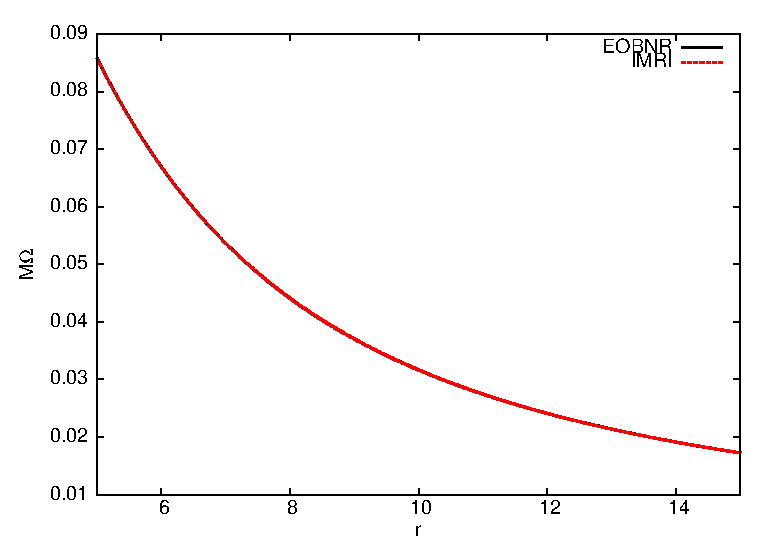
\includegraphics[height=0.35\textwidth,  clip]{figures/insimri/rom17100bold}
\includegraphics[height=0.35\textwidth,  clip]{figures/insimri/rom10100bold}
% }
% \centerline{
\includegraphics[height=0.35\textwidth,  clip]{figures/insimri/rom1100bold}
\includegraphics[height=0.35\textwidth,  clip]{figures/insimri/omac}
% }
\caption{The panels show the orbital frequency, as a function of the radial coordinate \(r\),  obtained using the fit described in the text (solid red line), and the orbital frequency predicted by the EOB model (solid black line). The systems shown in the panels correspond to binaries of component masses \(17 M_{\odot}+100M_{\odot}\) (top-left panel), \(10 M_{\odot}+100M_{\odot}\) (top-right) and  \(1 M_{\odot}+100M_{\odot}\) (bottom-left panel). The bottom-right panel demonstrates the accuracy with which our IMRI model reproduces the orbital frequency predicted by the EOBNRv2 for the systems 17:100 (dashed blue), 10:100 (dashed-dot red) and 1:100 (solid black). Note that the spikes are due to artifacts in the interpolation function used to plot the EOBNRv2 orbital frequency and the numerical fit used to reproduce it. Also notice that the discrepancy between the data and the fit is always smaller than one part in a thousand. }
\label{omegafit}
\end{figure*}

We next require a prescription to generate the inspiralling trajectory of the stellar mass compact object. The first step to achieve this consists of deriving a consistent model for the flux of angular momentum, which is discussed in the following section.
% The model for the flux of angular momentum that we introduce in the following Section sums up the effect of including all the dominant and subdominant modes currently available in the literature, i.e., \(2\leq \ell \leq 8, \, 1\leq m \leq \ell\), with the advantage of reduced computational cost.


\subsection{Radial evolution prescription}

An important component of the IMRI waveform model is the prescription used for the fluxes of energy and angular momentum. Deriving an accurate expression for these quantities is essential to capture the main features of true inspirals, as shown in \cite{improved} in the context of EMRIs. 


As discussed in Section~\ref{ssec:EOB}, in the EOBNRv2 model the flux of energy is constructed using the prescription given by Eq.~\eqref{eq:EOBdEdt}, which is obtained by summing over the modes  \(( h_{\ell m}\)) with \(2\leq \ell \leq 8\), \(1\leq m\leq \ell\). Using this prescription as input data and the fact that in the EOB formalism the following relation is fulfilled~\cite{barus}

\begin{equation}
\dot E= \Omega\dot L_z,
\label{circr}
\end{equation}

\noindent we derive a prescription for the gravitational-wave angular momentum flux which is valid from early inspiral all the way to the ISCO and slightly beyond.  This prescription, which encapsulates the contribution from 35 dominant and subdominant modes, is inspired by the modeling of accurate EMRI waveform models introduced in~\cite{improved}, i.e., 

\begin{equation}
\left(\dot L_z\right)_{\rm fit} = -\frac{32}{5}\frac{\mu^2}{M}\frac{1}{r^{7/2}}\Bigg[1-\frac{1247}{336}\frac{1}{r}+4\pi\frac{1}{r^{3/2}}- \frac{44711}{9072}\frac{1}{r^2} + \frac{1}{r^{5/2}}\left(c^1_{2.5} +  c^2_{3}\frac{1}{r^{1/2}}+c^3_{3.5}\frac{1}{r}\right)\Bigg],
\label{lzfluxfit}
\end{equation}

\noindent and the coefficients in Eq.~\eqref{lzfluxfit} are given in Table~\ref{Lzdotcoef}.

\begin{table}[ht]
\centering
\begin{tabular}{c c c c}
\hline\hline
  $\eta$& $c^1_{2.5}$ & $c^2_{3}$ & $c^3_{3.5}$   \\  
    $\frac{1700}{13689}$& -121.903 & 551.141 &-694.699  \\ [1ex]
   $\frac{10}{121}$& -110.657 & 360.261 &-156.016 \\ [1ex]
    $\frac{100}{10201}$&-75.255 & 333.449 & -363.505  \\ [1ex]
\hline
\end{tabular}
\caption{\(\dot{L}_z\) fit coefficients}
\label{Lzdotcoef}
\end{table}


Figure~\ref{fluxfitlight} provides a comparison between the EOBNRv2 flux and the calibrated angular momentum flux \(\left(\dot L_z\right)\). Notice that our modeling scheme does pretty well from large \(r\) all the way to the ISCO and slightly beyond. Hence, this approach will enable us to capture the main features of the inspiral evolution of the systems under consideration in the regime of interest with good accuracy. Modelling the prescription of the flux of angular momentum in our IMRI waveform using all the dominant and subdominant modes in the EOBNRv2 model is equivalent to modeling the radiative part of the self-force with the best information currently available in the literature. 



\begin{figure*}%[ht]
% \centerline{
\includegraphics[height=0.35\textwidth,  clip]{figures/insimri/lzdotp17100}
\includegraphics[height=0.35\textwidth,  clip]{figures/insimri/lzdotp10100}
% }
% \centerline{
\includegraphics[height=0.35\textwidth,  clip]{figures/insimri/lzdotp1100}
\includegraphics[height=0.35\textwidth,  clip]{figures/insimri/facc}
% }
\caption{We compare the calibrated flux of angular momentum described in Eq.~\eqref{lzfluxfit} against the prediction of the EOBNRv2 model for binaries of component masses \(17M_{\odot} + 100M_{\odot}\) (top left panel),  \(10M_{\odot} + 100M_{\odot}\) (top right panel), and \(1M_{\odot} + 100M_{\odot}\) (bottom-left panel). The bottom-right panel shows the accuracy with which the IMRI model reproduces the EOBNRv2 angular momentum flux, \(\dot{L}=dL_z/dt\), for the systems: 17:100 (dashed blue), 10:100 (dashed-dot red) and 1:100 (solid black). The spikes in the bottom-right panel are due to numerical artifacts of the interpolating function used to plot the EOBNRv2 angular momentum flux and the numerical fit to reproduce it. The fit is such that its discrepancy to the EOBNRv2  is always smaller than one part in a thousand.}
\label{fluxfitlight}
\end{figure*}


In Figure~\ref{fluxfitheavy} we present a comparison between the flux of angular momentum predicted by the EOBNRv2 model and the fit to Teukolsky data proposed in \cite{improved} for extreme-mass-ratio inspirals. Note the remarkable agreement between both formalisms all the way down to the ISCO. This comparison also confirms that the construction of the EOBNRv2 captures the main features of inspirals with small mass-ratios which are modeled using black hole perturbation theory. This comparison also shows that the EOBNRv2 model encodes fairly well the radiative part of the self-force for systems with small mass-ratio. 


\begin{figure*}%[ht]
% \centerline{
\includegraphics[height=0.6\textwidth,  clip]{figures/insimri/TEOBLzdot}
\includegraphics[height=0.5\textwidth,  clip]{figures/insimri/teuvseobflux}
% }
\caption{The top panel shows the angular momentum flux for binaries of mass ratio 1:100 computed using the EOBNRv2 model and the fit to Teukolsky data introduced in \cite{improved}. Both formalisms present a remarkable agreement all the way down to the ISCO. Note that the angular momentum flux fit to Teukolsky data is valid only from early inspiral until the ISCO. The bottom panel shows the relative difference between the two prescriptions for the angular momentum flux \(\dot{L}=dL_z/dt\).}
\label{fluxfitheavy}
\end{figure*}


Having found a prescription for the angular momentum that captures the dynamics of IMRIs, we can now use it to generate the inspiral trajectory of the stellar mass compact object that inspirals into an IMBH using the relation 

\begin{equation}
\frac{d r}{d t}= \frac{d L_z}{d t}\frac{d r}{d L_z}.
\label{drdt}
\end{equation}

\noindent  The first term on the right hand side of Eq.~\eqref{drdt} can be obtained from Eq.~\eqref{lzfluxfit}. With regard to the derivative of the angular momentum with respect to the radial coordinate, we need to use a prescription for the angular momentum that goes beyond the test-mass particle limit, as conservative self-force corrections play a more significant role in this regime. Hence, we use the relation derived by Barausse et al in \cite{barus} which includes conservative self-force corrections, i.e.,

\begin{equation}
\hat{L}_z (x)= \frac{L_z}{\mu M}= \frac{1}{\sqrt{x(1-3x)}} + \eta\left(-\frac{1}{3 \sqrt{x}} z'_{\rm SF}(x) + \frac{1}{6\sqrt{x}}\frac{4-15x}{\left(1-3x\right)^{3/2}}\right) + {\cal O} (\eta^2),
\label{angmom}
\end{equation}

\noindent where \(x=(M\Omega)^{2/3}\) and \('\) stands for \(d/dx\). Furthermore,

\begin{equation}
z_{\rm SF} (x)= 2x \frac{1+b_1 x+b_2 x^2}{1+b_3x +b_4 x^2 + b_5 x^3},
\label{zedsf}
\end{equation}

\noindent and the various coefficients \(b_i\) were derived in \cite{barus} using available self-force data. In this section we derive the coefficients in Eq.~\eqref{zedsf} that reproduce the actual inspiral evolution all the way down to the ISCO. Note that in Eq.~\eqref{drdt} we have in place a prescription for the angular momentum flux which faithfully reproduces the expected loss of angular momentum even beyond the ISCO,  as compared to the EOBNRv2 model. Hence, the only ingredient that needs to be tuned to reproduce the expected inspiral evolution is contained in Eq.~\eqref{angmom}. We have followed this approach to explore the form that \(\hat{L}_z (x)\) should have. Put in different words, the form that the self-force redshift observable \(z_{\rm SF} (x)\) should have to reproduce an inspiral trajectory consistent with EOBNRv2 all the way down to the ISCO.  The various coefficients of Eq.~\eqref{zedsf} that generate such an inspiral orbit are given in Table~\ref{zedfunccoef}.

\begin{table}[ht]
\centering
\begin{tabular}{c c c c c c}
\hline\hline
  $\eta$& $b_1$ & $b_2$ & $b_3$ & $b_4$ & $ b_5 $  \\  
    $\frac{1700}{13689}$& -3.062 & 0.760 & -3.261 & 0.550 & -6.000 \\ [1ex]
   $\frac{10}{121}$& -3.260 & 0.892 & -3.475 & 0.600 & -6.829\\ [1ex]
    $\frac{100}{10201}$&-3.370 & 1.570 & -3.730 & 0.970 & -7.280 \\ [1ex]
\hline
\end{tabular}
\caption{\(z_{\rm SF} (x)\) fit coefficients}
\label{zedfunccoef}
\end{table}

In Figure~\ref{dv15100} we show that this prescription captures with great accuracy the features of EOBNRv2  inspirals. To recap,  the IMRI model incorporates both first-order conservative corrections --through  the construction of the gauge invariant expression of the angular momentum in  Eq.~\eqref{angmom}--- and first-order radiative-corrections through the construction of the flux of angular momentum in Eq.~\eqref{lzfluxfit}. 
% Using this IMRI model, we have been able to constrain the form of the angular momentum \(L_z(x)\) that reproduces the inspiral evolution predicted by the EOBNRv2 model.

\begin{figure*}%[ht]
\centerline{
\includegraphics[height=0.38\textwidth,  clip]{figures/insimri/tphiim17100k}
\includegraphics[height=0.38\textwidth,  clip]{figures/insimri/rtim17100k}
}
\centerline{
\includegraphics[height=0.38\textwidth,  clip]{figures/insimri/tphiim10100k}
\includegraphics[height=0.38\textwidth,  clip]{figures/insimri/rtim10100k}
}
\centerline{
\includegraphics[height=0.38\textwidth,  clip]{figures/insimri/tphiim1100k}
\includegraphics[height=0.38\textwidth,  clip]{figures/insimri/trim1100k}
}
\caption{The panels show the radial and azimuthal evolution for a \(17M_{\odot} + 100M_{\odot}\) system (top panels), \(10M_{\odot} + 100M_{\odot}\) system (middle panels), and \(1M_{\odot} + 100M_{\odot}\) system (bottom panels), obtained using the IMRI model compared against the EOBNRv2 model.}
\label{dv15100}
\end{figure*}

\begin{figure*}%[ht]
% \centerline{
\includegraphics[height=0.6\textwidth,  clip]{figures/insimri/radacc}
\includegraphics[height=0.6\textwidth,  clip]{figures/insimri/phaacc}
% }
\caption{The panels show the accuracy with which the IMRI model proposed in the chapter reproduces the radial (top panel) and azimuthal (bottom-panel) time evolution predicted by the EOBNRv2 model for the systems  \(17M_{\odot} + 100M_{\odot}\) (dashed blue), \(10M_{\odot} + 100M_{\odot}\) (dashed-dot red), and \(1M_{\odot} + 100M_{\odot}\) (solid black). Notice that our model reproduces the EOBNRv2 orbital and azimuthal evolution point to point with an accuracy better than  one part in a thousand. }
\label{randphiaccuracy}
\end{figure*}



In order to show the importance of increasing our knowledge of the self-force in the intermediate-mass-ratio regime, we present in Figure~\ref{emimcomp}  three different curves which describe the time evolution of three binary systems during late inspiral. These plots show that if we use a waveform model (unfitted) that includes: a) an accurate prescription for the orbital frequency \(\hat\Omega\); b) a prescription for the flux of angular momentum that incorporates the contribution from all dominant and subdominant \((\ell,m)\) modes; c) an invariant expression for the angular momentum using the object \(x=\hat\Omega^{2/3}\) (see  Eq.~\eqref{angmom}), and; d) available self-force corrections to constrain the coefficients \(b_i\)~\cite{barus}, then such a model would generate an inspiral trajectory that deviates from the expected orbital evolution, in particular near the ISCO. 


Figure~\ref{emimcomp} also shows that our model actually predicts the expected orbital evolution all the way down to the ISCO, in agreement with the EOBNRv2 model, and requires a different set of coefficients  \(b_i\) in the redshift observable \(z_{\rm SF} (x)\), as compared with results in the extreme-mass-ratio limit quoted in~\cite{barus}. Notice that this is not only a modeling issue. It is an indication that implementing available self-force data into IMRI waveform models will not render the correct inspiral evolution, at the very  least for the cases we have considered. This is an important result of this chapter. In order to substantiate this statement, in the following Section we will compute the value of the gauge invariant angular momentum \(L_z(x)\) at the ISCO within both the self-force formalism and our IMRI model. We will also show that the evolution of \(L_z(x)\) is consistent between both formalisms during early inspiral, but that the form of this object differs as we near the ISCO.  

One may also expect that for binaries with small mass-ratios, available self-force corrections may provide a fairly good description of the inspiral evolution. This is what we actually see in the bottom panel of Figure~\ref{emimcomp}. We will also show in the following Section that the evolution of \(L_z(x)\) for binaries with mass-ratio 1:100 is consistent from early inspiral to the ISCO with EOBNRv2. This may not be surprising, since current self-force data have been obtained in the context of EMRIs and the EOBNRv2 has been calibrated so as to reproduce the dynamical evolution of binary black holes of small mass-ratio~\cite{resu,raci,nic,nic1}. This exercise then suggests that it may be necessary to go beyond first-order conservative corrections to reproduce accurately the expected dynamical evolution of intermediate-mass ratio systems with \(\eta \sim 10^{-2}-10^{-1}\).



\begin{figure*}%[ht]
% \centerline{
\includegraphics[height=0.35\textwidth,  clip]{figures/insimri/imem17100comp}
\includegraphics[height=0.35\textwidth,  clip]{figures/insimri/imem10100comptwo}
% }
% \centerline{
\includegraphics[height=0.35\textwidth,  clip]{figures/insimri/imem1100comp}
\includegraphics[height=0.35\textwidth,  clip]{figures/insimri/radaccemri}
% }
\caption{The panels show the radial evolution using the EOBNRv2 model, the IMRI model described in the text, and a model (Unfitted) which is the same as the IMRI model described in text except for the fact that the coefficients used in Eq.~\eqref{zedsf} for the function  \(z_{\rm SF} (x)\) were derived using available self-force data from extreme-mass ratio calculations~\cite{barus}. The plots correspond to binaries of component masses \(17M_{\odot} + 100M_{\odot}\) (top-left panel), \(10M_{\odot} + 100M_{\odot}\) (top-right panel) and \(1M_{\odot} + 100M_{\odot}\) (bottom-left panel). The bottom-right panel shows that the orbital evolution predicted by a model that incorporates self-force corrections from extreme-mass-ratio inspirals (EMRIs) deviates from the orbital evolution predicted by the EOBNRv2 model at late inspiral. This discrepancy is more noticeable for systems with mass-ratios 17:100 (dashed blue) and 10:100 (dashed-dot red). Furthermore, for smaller mass-ratios, 1:100 (solid black), the 
discrepancy becomes comparatively smaller, as expected. }
\label{emimcomp}
\end{figure*}



To carry out the analysis described above in the following Section, we will start by using the EOBNRv2 model to compute the orbital frequency ISCO shift for binaries of mass ratio 1:1, 1:2, 1:3, 1:4, 1:5, 1:6, 1:10 and 1:100, along with perturbative results in the context of extreme-mass-ratio inspirals. We will use this expression for the orbital frequency ISCO shift  to evaluate the gauge-invariant object \(x\)  and then compute the value of the angular momentum at the ISCO using Eq.~\eqref{angmom}.  We should also acknowledge the fact that EOB has not yet been calibrated using NR simulations of systems with mass-ratio 1:100. It is expected that EOBNRv2 provides a fair description of the dynamical evolution of such sources,  and we show in the following section that both EOBNRv2 and perturbative calculations provide a consistent modeling of the gauge-invariant angular momentum \(\hat{L}_{z}\) from early inspiral to the ISCO for binaries with mass-ratio 1:100. However, this study should be 
compared to accurate NR simulations of mass-ratio 1:100~\cite{carlos} when available in sufficient length.


% \clearpage


\section{ISCO shift: connecting the extreme, intermediate and comparable-mass ratio regimes}
\label{s3}

In the previous Sections we have mentioned that during the inspiral of a stellar mass compact object of mass \(m_2\) into a supermassive BH of mass \(m_1\), the radiative part of the self-force drives the inspiral evolution of the small object, whereas its conservative part has a cumulative effect on the orbital phase evolution \cite{SFB}. These two effects have been considered in the development of EMRI waveform templates  \cite{amos, cutler, gairles, kludge, improved, lisacapt, seoane}. 

We shall now consider a novel effect that was explored by Barack \& Sago~\cite{inner}. They have shown that the self-force also introduces shifts in the innermost stable circular orbit radius and frequency. For a test-mass particle, these two quantities are given by

\begin{equation}
r_{\rm ISCO} = 6m_1,  \qquad m_1\Omega_{\rm ISCO} = \frac{1}{6\sqrt{6}},
\label{tmpt}
\end{equation}

\noindent whereas, for finite \(\eta\), in the Lorenz gauge, these two quantities take the form~\cite{inner} 

\begin{equation}
\Delta r_{\rm ISCO} = -3.269(\pm3\times10^{-3}) m_2,  \qquad \frac{\Delta\Omega_{\rm ISCO}}{\Omega_{\rm ISCO}} = 0.4870(\pm6\times10^{-4})\frac{m_2}{m_1}.
\label{shift}
\end{equation}

Since Barack \& Sago carried out these calculations in Lorenz gauge, it was necessary to translate these results into coordinates that are commonly used for GW observations, i.e., asymptotically flat coordinates.  This exercise has been done for the orbital frequency, which is a gauge invariant object, and hence can be compared to results obtained in alternative formalisms, such as PN theory or the EOB approach.  In \cite{baracknewphi} and \cite{damsh}, the authors derive the `renormalization' factor that translates results of Lorenz-gauge calculations into  physical units. Applying this renormalization technique, one finds that the ISCO frequency is given by  

\begin{equation}
M\Omega_{\rm ISCO} = \frac{1}{6\sqrt{6}}\left(1+1.2512\eta + {\cal{O}}(\eta^2)\right),
\label{bsshift}
\end{equation}

\noindent with \(M=m_1+m_2\). This prediction can be compared with PN--based ISCO calculations at different orders of accuracy \cite{favata}

\begin{eqnarray}
M\Omega^{2{\rm PN}}_{\rm ISCO} &=&\frac{1}{6\sqrt{6}}\left(1+\frac{7}{12}\eta + {\cal{O}}(\eta^2)\right), \\\nonumber
M\Omega^{3{\rm PN}}_{\rm ISCO} &=&\frac{1}{6\sqrt{6}}\left(1+ \left(\frac{565}{288} - \frac{41}{768}\pi^2\right)\eta + {\cal{O}}(\eta^2)\right). \\\nonumber
\label{pnshift}
\end{eqnarray}

\noindent The EOB approach has also been used to describe the orbital frequency shift at ISCO. Damour suggested in \cite{damsh} that a fit for the ISCO orbital frequency shift that incorporates results from the gravitational self-force and NR simulations may be a quadratic polynomial in \(\eta\) of the form \cite{damsh} 

\begin{equation}
M\Omega^{\rm Damour}_{\rm ISCO} = \frac{1}{6\sqrt{6}}\left(1+1.25\eta + 1.87\eta^2\right).
\label{damshift}
\end{equation}


\noindent In this chapter we build up on this analysis and update this estimate using results from the self-force program, and making use of the EOBNRv2 model, which has been calibrated to NR simulations~\cite{BuonannoEOBv2Main}. The prescription for the orbital frequency ISCO shift that we propose below reproduces accurately the results predicted by the self-force program for EMRIs, and also reproduces the best data currently available for intermediate and comparable-mass systems.  To compute the ISCO orbital frequency shift, we use the equation derived in \cite{damsh}, namely,


\begin{equation}
2A(u)A'(u) + 4u\left(A'(u)\right)^2 - 2uA(u)A''(u)=0,
\label{damisco}
\end{equation}

\noindent where \(u=1/r\) and \('\) stands for \(d/du\), as before. 
This ISCO condition can be rewritten in terms of the radial coordinate as \cite{favata}

\begin{equation}
rA(r)A''(r) -2r\left(A'(r)\right)^2 +3A(r)A'(r)=0,
\label{iscoeq}
\end{equation}

\noindent where \('=d/dr\). We shall use the metric coefficient \(A(r)\) quoted in \cite{BuonannoEOBv2Main}, which includes the Pad\'e expression for \(A(r)\) at 5PN order.  Having obtained the value for \(r_{\rm  isco}\) using Eq.~\eqref{iscoeq}, we evaluate the angular orbital frequency  \(M\Omega_{\rm ISCO}\) at  this fiducial value using Eq. (10b) of \cite{BuonannoEOBv2Main} with \(p_r =0\). 

Using a variety of events, including extreme, \(\eta\sim 10^{-5}\), and intermediate, \(\eta\sim 10^{-2}-10^{-1}\), mass ratio inspirals, we derive a quadratic polynomial fit  in \(\eta\) for the ISCO orbital frequency shift for these types of events, namely

\begin{equation}
M\Omega^{\rm fit}_{\rm ISCO} = \frac{1}{6\sqrt{6}}\left(1+1.05786\eta + 2.12991\eta ^2\right).
\label{newshift}
\end{equation}

\noindent We found that at second order in \(\eta\), this numerical fit does not reproduce accurately the orbital frequency ISCO shift for small-mass ratios~\cite{inner}. We can fix these problems using a prescription of the form

\begin{equation}
M\Omega^{\rm fit}_{\rm ISCO} = \frac{1}{6\sqrt{6}}\left(1 + 1.2512\eta - 0.0553751\eta^2 + 5.78557\eta^3\right).
\label{comisco}
\end{equation}

\noindent At this level of accuracy we exactly reproduce the prediction for EMRIs for small \(\eta\), as well as the most-up-to-date results for binaries modeled using the EOBNRv2 scheme. We compare the range of applicability of this numerical expression, along the other various approximations mentioned above,  in Figure~\ref{iscoshift}.

 
\begin{figure*}%[ht]
\centerline{
\includegraphics[height=0.8\textwidth,  clip]{figures/insimri/mwiscotwo}
}
\caption{ISCO shift using various approximations as described in the text. The `Numerical Data' has been obtained using calculations in the extreme-mass ratio regime~\cite{inner} and the EOBNRv2. The prescription that encapsulates results from the extreme, intermediate and comparable mass-ratio regime is labeled as `Numerical Fit' and is given by Eq.~\eqref{comisco} in the main text.  }
\label{iscoshift}
\end{figure*}


With our prescription for \(M\Omega_{\rm ISCO}\), we can evaluate the value of the gauge-invariant angular momentum at the ISCO. To do so, we first use Eq.~\eqref{bsshift} to compute the shift in the orbital frequency at the ISCO, and then use Eq.~\eqref{angmom} in conjunction with the values for the \(b_i\) coefficients of Eq.~\eqref{zedsf} calculated in the EMRI limit~\cite{barus}. We also present results for an `incomplete model', in which we use Eq.~\eqref{comisco} to evaluate the value of the orbital frequency at the ISCO, and then use Eq.~\eqref{angmom} with the set of \(b_i\) coefficients quoted in~\cite{barus}. Finally, we use the prescription for the shift of the orbital frequency at the ISCO in Eq.~\eqref{comisco}, and the prescription for the angular momentum (Eq.~\eqref{angmom}) using the corrections quoted in Table~\ref{zedfunccoef}. 
Table~\ref{lzcomp} shows that, in accord with Figure~\ref{emimcomp}, for binaries with symmetric mass-ratio \(\eta \sim 0.01\), the value of the angular momentum evaluated at ISCO is fairly consistent between the two models. However,  the predicted value of the angular momentum at ISCO becomes more discrepant for binaries with   \(\eta \sim 0.1\). This further affirms that the evolution of intermediate-mass ratio inspirals cannot be fully captured by using self-force calculations from extreme-mass ratio inspirals. This can be better visualized in Figure~\ref{lzfull} where we show the angular momentum during inspiral all the way down to the ISCO using two formalism, namely, our IMRI prescription and a model that includes only available self-force corrections (labeled as `Self Force'). 


\begin{table}%[thb]
\begin{center}
\begin{tabular}{|c|c|c|c|}
\hline\multicolumn{1}{|c|}{}&\multicolumn{3}{c|}{\(L_z(x_{\rm ISCO} )\)}\\\cline{2-4}
\multicolumn{1}{|c|}{\(\eta\)}&SF Fit&Incomplete&IMRI \\\cline{1-4}
$\frac{1700}{13689}$&3.3389 &3.3522&3.2918 \\[1ex]\cline{1-4}
$\frac{10}{121}$& 3.3876&3.3878&3.3254\\ [1ex]\cline{1-4}
$\frac{100}{10201}$& 3.4561&3.4561&3.4429\\[1ex]\hline
\end{tabular}
\caption{ The Table shows the value of the angular momentum \(L_z\) as a function of the gauge invariant object \(x=\left(M\Omega \right)^{2/3}\)  evaluated at the ISCO radius (see Eq.~\eqref{angmom}). The SF (self-force) values are computed using the prescription given in Eq.~\eqref{bsshift} to compute the orbital frequency shift, and Eq.~\eqref{angmom} with the coefficients \(b_i\) quoted in \cite{barus}, i.e., evaluated in the context of extreme-mass-ratio inspirals. Incomplete stands for a prescription in which we use the prescription for the orbital frequency given by Eq.~\eqref{comisco}, and the angular momentum prescription given by  Eq.~\eqref{angmom} with the coefficients \(b_i\) quoted in \cite{barus}. The   \(b_i\) values of the IMRI model are obtained using a model that reproduces the dynamical evolution of intermediate-mass-ratio inspirals, as compared with the EOBNRv2 model, and for which we have derived a new prescription for the red-shift observable \(z_{\rm SF} (x)\) which actually 
reproduces the features of true inspirals.}
\label{lzcomp}
\end{center}
\end{table}


\begin{figure*}[ht]
% \centerline{
\includegraphics[height=0.35\textwidth,  clip]{figures/insimri/lz17100invbold}
\includegraphics[height=0.35\textwidth,  clip]{figures/insimri/lz10100invbold}
% }
% \centerline{
\includegraphics[height=0.35\textwidth,  clip]{figures/insimri/lz1100invbold}
\includegraphics[height=0.35\textwidth,  clip]{figures/insimri/angmomacc}
% }
\caption{The panels show the invariant angular momentum \(L_{z}(x)\), with \(x=\left(M\Omega\right)^{2/3}\), from early inspiral to the ISCO using two different prescriptions. The `IMRI' prescription reproduces accurately the expected inspiral evolution, as compared with results from the EOBNRv2 model ---which has been calibrated to NR simulations. The `Self-Force' prescription encapsulates self-force corrections derived in the context of EMRIs~\cite{sago,barus}. Note that for the three binary systems studied,  \(17M_{\odot} + 100M_{\odot}\) (top-left panel),  \(10M_{\odot} + 100M_{\odot}\) (top-right panel), and  \(1M_{\odot} + 100M_{\odot}\) (bottom-left panel), the `Self Force' prescription for the angular momentum presents a deviation from its expected value that becomes more noticeable near the ISCO. The bottom-right panel shows the fractional accuracy between the two different prescriptions for the angular momentum for the systems 17:100 (dashed blue), 10:100 (dashed-dot red) and 1:100 (solid black). 
Notice also that, as expected, for binaries with small mass-ratio the `Self Force' and `IMRI' prescriptions are fairly consistent all the way down to the ISCO.  As in the previous plots, the spikes in the bottom-right panel are due to numerical artifacts.}
\label{lzfull}
\end{figure*}

Table~\ref{lzcomp} and Figures~\ref{emimcomp}, \ref{lzfull} show that as the mass-ratio increases, the discrepancy between a model that incorporates available self-force corrections~\cite{sago} and one that has been calibrated to NR simulations becomes more pronounced. For events with mass-ratio 1:10 this difference looks slightly larger than for those of mass-ratio 17:100. Part of the reason for this behavior may be the fact that the model we have used to perform this analysis, EOBNRv2, provides the best prescription currently available for the inspiral evolution of sources with mass-ratios 1:1-1:6. It is expected that the model provides a good description of the inspiral evolution of sources with mass-ratio 1:10, and hence we have extended its realm of applicability to shed light on the form that the self-force is expected to have so as to reproduce the inspiral evolution of these type of sources. Thus, a conservative conclusion we can draw at this stage is that, using the best waveform model currently 
available in the literature, we have shown that  one may not be able to accurately model the dynamics of sources with mass-ratio 1:10 using available self-force calculations.  This trend is also present   in the case of events with mass-ratio 17:100 and the results in this case are more conclusive. We have shown that a waveform model that includes available self-force corrections will not be able to capture faithfully the inspiral evolution of these GW sources. These results suggest that one may need to include higher-order corrections in the self-force to capture the behavior of true inspirals in the intermediate-mass-ratio regime. 
% Finally, our work is also a consistency check on the internal structure of the EOB model, since we have shown that the EOBNRv2 renders a good prescription for the inspiral evolution via the flux of angular momentum and that the angular momentum prescription is consistent with results obtained from perturbative calculations. 
% % \clearpage

 
  
\section{Extension to equal-mass binaries}

In this Section we show that the approach outlined in the main body of the chapter can still be used to model equal-mass (EM) binaries with great accuracy at an inexpensive computational cost. To do so we consider a system with total mass \(20 M_{\odot}\). Following the method described in Section~\ref{s2}, we start by deriving accurate prescriptions for the orbital frequency \(\Omega_{\rm ansatz}\) and angular momentum flux \(\dot{L}_z\). Thereafter we derive the corrections that should be implemented in the gauge-invariant expression for the angular momentum (see Eq.~\eqref{angmom}) to accurately reproduce the inspiral evolution predicted by the EOBNRv2 model. 

\begin{figure*}[ht]
% \centerline{
\includegraphics[height=0.32\textwidth]{figures/insimri/anfreemc}
\includegraphics[height=0.32\textwidth]{figures/insimri/amfemc}
% }
% \centerline{
\includegraphics[height=0.32\textwidth,  clip]{figures/insimri/rteobvsemc}
\includegraphics[height=0.32\textwidth,  clip]{figures/insimri/phiteobvsem}
% }
% \centerline{
\includegraphics[height=0.32\textwidth,  clip]{figures/insimri/lzinveobvcem}
% }
\caption{The panels show the accuracy with which our model can reproduce the dynamics of an equal mass (EM) binary system with masses  ( \(10M_{\odot} + 10M_{\odot}\)), as compared with the EOBNRv2 model. The top panels show that our model can reproduce the orbital angular evolution and the flux of angular momentum predicted by the EOBNRv2 model point to point with an accuracy better than one part in a thousand. The middle panels show that our model can reproduce with a similar accuracy the radial and azimuthal evolution of a   \(10M_{\odot} + 10M_{\odot}\) binary system. The bottom panel shows that the expression for the gauge-invariant angular momentum \(L_{z}(x)\) for an EM mass deviates clearly from the EMRI prescription even before nearing the ISCO. }
\label{emcase}
\end{figure*}

The prescriptions for the orbital frequency, angular momentum flux and angular momentum which reproduce the inspiral evolution for the \(10M_{\odot} + 10M_{\odot}\) binary system shown in Figure~\ref{emcase} require the following set of coefficients (compare Tables~\ref{coef}, \ref{Lzdotcoef}, \ref{zedfunccoef})


\begin{equation}
\begin{split}
\Omega(u)_{\rm ansatz} &: a_1= -5.644, \quad a_2 = 11.003, \quad a_3 = -5.390,\quad a_4 = 8.794, \quad a_5 = 0.458\\
\dot{L}_z &: c^{1}_{2.5} = -90.566, \quad c^2_3  =304.941, \quad c^3_{3.5}= -339.500\\
z_{\rm SF} &:  b_1 = -5.803,\quad  b_2= 14.171, \quad b_3 = -7.074, \quad b_4 = 22.810, \quad b_5 =-25.580
\label{ecmcoe}
\end{split}
\end{equation}

Having shown that the approach outlined in the chapter is still effective to model EM binaries, we consider worthwhile developing a model that encapsulates the physics of binaries of comparable and intermediate-mass-ratio. In order to extend our IMRI model into the comparable mass-ratio regime, we will require some changes in the model.  First and foremost, we require expressions for the orbital frequency evolution (see Eq.~\eqref{ompres}) and angular momentum (see Eq.~\eqref{angmom}) which incorporate conservative corrections at second-order in mass ratio \(\eta\). We can draw this conclusion by comparing the bottom-right panel of Figure~\ref{lzfull} with the bottom panel of Figure~\ref{emcase}. The former plot shows that for IMRIs the prescription for the angular momentum  deviates from the self-force prediction near the ISCO. However, the latter plot shows that in the EM case the prescription for the angular momentum deviates considerably from the self-force prediction even during the inspiral 
evolution, far away from the ISCO. Because the prescription we have used for the angular momentum in both cases includes corrections at liner order in mass-ratio, this suggest that to derive a model that unifies both regimes we require  an expression for the angular momentum which includes second-order conservative corrections. We can follow a similar strategy to encapsulate in a single prescription the radiative piece of the self-force for comparable and intermediate mass-ratio systems by deriving second-order radiative corrections in the prescription for the angular momentum flux. 

Once suitable expressions for \(\Omega_{\rm ansatz}\), \(\dot{L}_z\) and \(L_{z}(x)\) have been derived, we will be able to tune the coefficients of these objects and derive numerical fits for the coefficients in terms of the mass-ratio \(\eta\) of the system. This approach will provide a unified description for the inspiral evolution of IMRIs and comparable-mass systems. This will be the subject of future study.


 \section{Conclusions}
 \label{s4}
 
 In this chapter we have developed a code to reproduce the analysis presented in \cite{BuonannoEOBv2Main}. Using this code we generated the inspiral evolution of three different systems to perform an exploratory study of the importance of including accurate self-force corrections in search templates that aim to detect non-spinning intermediate-mass ratio inspirals. The choice of the systems to perform this study reflects the knowledge we have at present on the dynamical evolution of non-spinning BH binaries (\(17M_{\odot} + 100M_{\odot}\)), what we want to know (\(10 M_{\odot} + 100M_{\odot}\)), and a special system that  provides reassurance that the dynamics of intermediate-mass-ratio inspirals with typical mass-ratios \(\eta\sim 0.01\) can be captured using perturbative theory, as shown in \cite{carlos,ulr}. 
 
 The EOBNRv2 model we have used as a benchmark to carry out this study has the advantage of encoding the best information currently available of non-spinning BH binaries, is capable of reproducing the expected dynamics in the test-mass particle limit, and also includes corrections taken from self-force corrections in the extreme-mass-ratio limit. We have confirmed these statements for systems with  \(\eta\sim 0.01\) by showing  that the EOBNRv2 does predict the expected form of the angular momentum flux, as compared to Teukolsky data, as well as the evolution  of the gauge-invariant angular momentum, as compared to self-force data. 
 
In order to explore the form of the self-force in the intermediate-mass-ratio regime, we developed an IMRI model that reproduces the inspiral evolution predicted by the EOBNRv2 model, and which enable us to explore the form that the self-force should have in this mass-ratio regime so as to reproduce the binary's dynamical evolution as predicted by the best available interface to NR simulations. We have found that for systems with component masses  \(17M_{\odot} + 100M_{\odot}\), available self-force corrections do not accurately reproduce the inspiral evolution. We have shown that there is a clear deviation from the true inspiral trajectory near the ISCO. We have also explored this issue in greater detail by showing that the gauge-invariant angular momentum does deviate from the current self-force prediction near the ISCO. When we extend the realm of applicability of the EOBNRv2 to binaries of mass-ratio 1:10, we observe a similar behaviour.  This exploratory study then suggests that it may be necessary to 
extend conservative corrections beyond the linear order to accurately capture the true inspiral evolution for sources with intermediate-mass-ratio. Furthermore, once NR simulations of systems with mass-ratios 1:10, 1:15 and 1:100 have reached enough resolution near merger, we will be in a good position to calibrate the EOB model so as to reproduce the true dynamical evolution for these type of sources \cite{carlos, carlosI,carlosII}. Such a model will enable us to further probe the parameter space to develop IMRI models, as the one proposed in this chapter, that capture the features of true inspirals at a very inexpensive computational cost. 

We have also used our EOBNRv2 code to derive a prescription for the orbital frequency ISCO shift that encapsulates results from the extreme, intermediate and comparable-mass ratio regimes. Our prescription is the first in the literature that reproduces the self-force result in the appropriate limit.   We have made use of this new prescription to estimate the value of the angular momentum at the ISCO using our IMRI prescription and available self-force data. We have found a clear discrepancy for systems with mass-ratios \(\eta \sim 0.1\), but have confirmed that for systems with small mass ratios \(\eta\sim 0.01\) both predictions are fairly consistent. 

This study has also shed light on  a pressing issue that needs to be addressed before aLIGO begins observations, namely, at present we use templates  in searches for GW sources  whose actual dynamics are currently unknown. For instance, searches for BH binaries with total mass  \(25M_{\odot} - 200M_{\odot}\), and individual masses from \(3M_{\odot}\) to \(99M_{\odot}\) have been carried out, but not a single model has been calibrated using high-resolution NR simulations for mass-ratios smaller than 1:6. Hence, it is important that numerical relativists and search template developers interact more closely so as to run NR simulations which cover regions in parameter space where future GW detectors may detect GW sources. This meaningful interaction will be important from a theoretical perspective, as we will be able to further our knowledge of the self-force, and from a data analysis perspective, as we will be in a stronger position to develop accurate search templates for use in data analysis. 

The approach we have outlined in this chapter is the initial step to construct inspiral-merger-ringdown IMRI waveforms. Having derived a consistent prescription for the inspiral evolution, we can use a similar approach to that described in~\cite{ori} to include merger and ring-down in a physically consistent way. Developing complete IMRI waveforms may be useful for aLIGO data analysis, as they will provide the accuracy of more complex waveform models at an inexpensive computational cost.  


\Chapter{Self-forced evolutions of an implicit rotating source: 
a natural framework to model comparable and intermediate mass-ratio systems 
from inspiral through ringdown}
\label{ch:imrSFIMRI}
%%%%%%%%%%%%%%%%%%%%%%%%%%%%%%%%%%%%%%%%%%%%%%%%%%%%%%%%%%%%%%%%%%%%%%%%%%%%%%%
%%% Describe the IMR model for IMRIs.
%%%%%%%%%%%%%%%%%%%%%%%%%%%%%%%%%%%%%%%%%%%%%%%%%%%%%%%%%%%%%%%%%%%%%%%%%%%%%%%

%
\def\etal{{\it et al.}}  \def\ie{{\it i.e.}}  \def\eg{{\it e.g.}}
\def\lap{\hbox{${_{\displaystyle<}\atop^{\displaystyle\sim}}$}}
\def\gap{\hbox{${_{\displaystyle>}\atop^{\displaystyle\sim}}$}}
\def\lesssim{\mathrel{\hbox{\rlap{\hbox{\lower4pt\hbox{$\sim$}}}\hbox{$<$}}}}
\def\gtrsim{\mathrel{\hbox{\rlap{\hbox{\lower4pt\hbox{$\sim$}}}\hbox{$>$}}}}
\def\alt{\mathrel{\hbox{\rlap{\hbox{\lower4pt\hbox{$\sim$}}}\hbox{$<$}}}}
\def\agt{\mathrel{\hbox{\rlap{\hbox{\lower4pt\hbox{$\sim$}}}\hbox{$>$}}}}
\def\prd{{\it Phys. Rev.} D~}
\def\PRL{{\it Phys.Rev.} Lett~}
\def\apjl{{\it Astrophys. J.} Lett~}
\def\apj{{\it Astrophys. J.}}
\def\Msun{M_\odot}
\def\PRD{{\it Phys. Rev.} D~}
\def\CQG{{\it Class. Quantum Grav.}}
\def\aaps{{\it A\&AS~ }}
\def\pasj{{\it PASJ }}
\def\mnras{{\it MNRAS}} 
\def\aapr{{\it A\&ARv}}

\def\gta{\ifmmode {\mathbin{\lower 3pt\hbox   %> or of order
    {$\,\rlap{\raise 5pt\hbox{$\char'076$}}\mathchar"7218\,$}}}
    \else {${\mathbin{\lower 3pt\hbox
    {$\rlap{\raise 5pt\hbox{$\char'076$}}\mathchar"7218\,$}}}
    $}\fi}
\def\lta{\ifmmode {\,\mathbin{\lower 3pt\hbox   %< or of order
    {$\,\rlap{\raise 5pt\hbox{$\char'074$}}\mathchar"7218\,$}}}
    \else {${\mathbin{\lower 3pt\hbox
    {$\rlap{\raise 5pt\hbox{$\char'074$}}\mathchar"7218\,$}}}
    $}\fi}

%%%%%%%%%%%%%%%%%%%%%%%%%%%%%%%%%%%%%%%%%%%%%%%%%%%%%%%%%%%%%%%%%%%%%%%%%%%%%%%

\section{Introduction}   
The black hole (BH) mass function in the local Universe is a strongly bi-modal distribution that identifies two main families: stellar-mass BHs with typical masses \(\sim 10M_{\odot}\) observed in Galactic X-ray binaries~\cite{McClintock:2006} and, more recently, in globular clusters~\cite{Morscher:2013}, and supermassive BHs with masses \(\gtrsim 10^{5} M_{\odot}\) observed to be present in most galactic nuclei~\cite{Merloni:2008, Fukugita:2004}.  However, a population of X-ray sources with luminosities in excess of \(10^{39}\, \rm{ erg}\, \rm{s}^{-1} \) has recently been observed, and {\it{Chandra}} and {\it{XMM-Newton}} spectral observations of these ultra-luminous X-ray sources (ULXs) revealed cool disc signatures that were consistent with the presence of intermediate mass BHs (IMBHs) with masses \(10^{2-4} M_{\odot}\)~\cite{Miller:2004,Miller:2004b,Miller:2006_BOOK}. Subsequent observations have shown that these ULXs have spectral and temporal signatures that are not consistent with the sub-Eddington 
accretion regime that is expected for IMBHs at typical ULX luminosities. Rather, these later studies suggest that many ULXs are powered by super-Eddington accretion onto \(\lesssim 100 M_{\odot}\) BH remnants.  Nevertheless, recent work by Swartz et al.~\cite{Swartz:2011} has demonstrated that as well as the high mass X-ray binaries that characterise most ULXs, there is a subpopulation of ULXs that seem to be powered by a separate physical mechanism. These objects have typical luminosities \(L\gtrsim 10^{41}\, \rm{ erg}\, \rm{s}^{-1} \), which cannot be explained by close to maximal radiation from super-Eddington accretion onto massive BHs formed in low metallicity regions~\cite{Zampieri:2009, Belczynski:2010, Ohsuga:2011}. Several hyper-luminous X-ray sources, including M82 X-1, ESO 243-49 HLX-1, Cartwheel N10 and CXO J122518.6+144545, present the best indirect evidence for the existence of IMBHs~\cite{Matsumoto:2001,Farrel:2009,Wolter:2010,Jonker:2010}.  In particular, the colocation of M82 X-1 with a 
massive, young stellar cluster, the features if its power spectrum, and some reported transitions between a hard state and a thermal dominant state, make this object a strong IMBH candidate~\cite{Portegies:2004,Strohmayer:2003,Kaaret:2007,Feng:2010}.  Recent searches of archival {\it{Chandra}} and {\it{XMM-Newton}} data sets have also uncovered two new hyper-luminous X-ray sources with luminosities in excess of \(10^{39}\, \rm{ erg}\, \rm{s}^{-1} \). These sources are the most promising IMBH candidates currently known, although the highest possible super-Eddington accretion rate onto the largest permitted BH remnant cannot yet be ruled out~\cite{Sutton:2012}.  This increasing body of observational evidence~\cite{Trenti:2006,Coleman:2004}, and the fact that the existence of IMBHs provides a compelling explanation for the initial seeding of supermassive BHs present in most galactic nuclei~\cite{Volonteri:2010,Schneider:2002,Yu:2002} has revived the quest for these elusive objects.  

Since hyper-luminous X-ray sources are rare, and our knowledge about their astrophysical properties is still limited, we may have to use a different means to search for IMBHs in order to improve our knowledge about the channels that lead to the formation of these objects, and to shed light on their astrophysical properties, such as mass and spin distributions~\cite{mandel}. In this chapter we explore the use of observations in the gravitational wave (GW) spectrum to gain insight into the properties of IMBHs. 

The current upgrade of the Laser Interferometer Gravitational Wave Observatory (LIGO) and its international partners Virgo and Kagra~\cite{aLIGO, virgo,kagra}, will enable the detection of GWs from coalescences involving IMBHs with masses \(50 M_{\odot} \lesssim M \lesssim 500 M_{\odot}\), if these instruments achieve their target sensitivity down to the low-frequency cutoff at 10Hz (See Figure~\ref{ZDHP_promise})~\cite{ZDHP:2010}.  Advanced LIGO (aLIGO) and Advanced Virgo are expected to have greatest sensitivity in the 60Hz - 500Hz range, with a peak at \(\sim60\) Hz (see Figure~\ref{ZDHP_promise}). Proposed third generation detectors, such as the Einstein Telescope~\cite{Freise:2009}, which aim to extend the frequency range of ground-based detectors down to 1Hz, while also maintaining high frequency sensitivity up to 10kHz, will enhance our ability to search for GWs emitted by sources that involve BHs with masses between \(10^{2-4}M_{\odot}\)~\cite{etgair,Huerta:2011a,Huerta:2011b}. 


A promising channel for detection of IMBHs is through the emission of gravitational radiation during the coalescence of stellar-mass compact remnants --- neutron stars (NSs) or BHs --- with IMBHs in core-collapsed globular clusters. This expectation is backed up by numerical simulations of globular clusters~\cite{Taniguchi:2000,Miller:2002,Mouri:2002a,Mouri:2002b,Gultekin:2004,Gultekin:2006,Oleary:2006,Oleary:2007}  which suggest that IMBHs could undergo several collisions with stellar-mass compact remnants during the lifetime of the cluster through a variety of mechanisms, including gravitational radiation, Kozai resonances and binary exchange processes.  As discussed in~\cite{man}, the most likely mechanism for the formation of binaries involving a stellar-mass compact remnant and an IMBH is hardening via three body interactions, with an expected detection rate of \(\sim 1-10\, {\rm{yr}}^{-1}\) with ground-based observatories~\cite{man,Abadie:2010}. 

\begin{figure*}[ht]
\centerline{
\includegraphics[height=0.35\textwidth,  clip]{figures/imrimri/nc_normalized.eps}
}
\caption{The panel shows the expected sensitivity for two configurations of the Einstein Telescope (ET), namely, ETD (black), ETB (blue) and LIGO's Zero Detuned High Power (ZDHP) configuration (red). The vertical axis measures \(F_{\rm{normalized}} =  \left(f/f_{\rm{max}}\right)^{-7/6}\sqrt{S_n(f_{\rm{max}})/S_n(f)}\), where \(f_{\rm{max}}\) is the maximum of the corresponding power spectral density, \(S_n(f)\).
}
\label{ZDHP_promise}
\end{figure*}


The frequency of the dominant quadrupolar harmonic in the GWs emitted at the innermost stable circular orbit (ISCO) for a binary of non-spinning objects is 
\begin{equation}
f_{\rm{ISCO}}= 4.4 {\rm{kHz}} \left(\frac{M_{\odot}}{M}\right),
\label{fIMRIisco}
\end{equation}
\noindent so for a typical intermediate mass--ratio coalescence (IMRC) with total mass \(M\gtrsim 100 M_{\odot}\), advanced detectors will observe the late inspiral, merger and ringdown. However, the heaviest IMRCs, with masses $\gtrsim500M_\odot$, will coalesce out of band or at the low frequency limit of the bandwidth. Hence, merger and ringdown --- which intrinsically generate a signal-to-noise ratio (SNR) suppressed by a  factor of symmetric mass-ratio --- see Table~\ref{length} below ---  relative to the SNR generated during the inspiral phase--- will significantly contribute to the SNR of IMRCs over a considerable portion of the detectable mass-range~\cite{Smith:2013}. In order to get the most information from GW observations of IMRCs, it is therefore necessary to develop waveform models that incorporate the inspiral, merger and ringdown in a physically consistent way. In order to make progress in this direction, we previously developed a waveform model that combined results from Black Hole 
Perturbation Theory (BHPT) and post-Newtonian (PN) theory to  explore the information that could be obtained from observations of IMRCs with the EinsteinTelescope~\cite{Huerta:2011a,Huerta:2011b}. Although this model provided an important step in exploring the science that could be done with IMRC observations, the model was limited.


In~\cite{Huerta:2009,Huerta:2010,Huerta:EHE,Huerta:2012} we explored using the self-force formalism~\cite{SFB,LRP} to develop a waveform model with a robust description of the dynamical evolution of IMRCs during the inspiral phase. These were found to be effective when used to carry out matched-filter based searches for inspiral-only IMRCs~\cite{Smith:2013}, but searches for IMRCs in the advanced detector era will require waveform models that include not only the inspiral but also the merger and ringdown~\cite{Smith:2013}. The model described in~\cite{Huerta:2011a} included merger and ring down but without the self-force driven inspiral. It would be ideal to develop a consistent inspiral, merger, ringdown waveform model by comparison to numerical relativity simulations, as described in~\cite{buho,Damour:2013}. However, numerical relativity simulations for systems with mass-ratios \(q=m_1/m_2 \lesssim 1/10\) are very computationally expensive at present~\cite{Mroue:2013}. We can circumvent this problem by 
making use of recent breakthroughs in the self-force program that have shown that the conservative part of the self-force can reproduce, with good accuracy, results from numerical relativity simulations of comparable-mass binary systems~\cite{LeTiec:2012}.   Furthermore, the recent computation of the self-force inside the ISCO equips us to now develop models that better reproduce the true dynamics of black hole binaries in the strong field regime~\cite{Akcay:2012}.  

In addition to IMRCs, which may be detected by second generation detectors, and with more likelihood by third generation detectors, we have explored the suitability of using self-forced evolutions to model the mergers of systems involving NSs and stellar mass BHs~\cite{LVCT}. Since NSBH mergers are promising GW sources for second generation detectors, we need to develop accurate and computationally inexpensive templates appropriate for these events. Current efforts to model NSBH systems have generally used PN approximants, evaluated to the highest post-Newtonian order available, but these approximates are not sufficiently reliable to model these events~\cite{pnbuo,Nitz:2013mxa}. In Figure~\ref{pn_approx}, we show the phase difference between the PN approximant TaylorT4~\cite{TaylorT4Origin} and the EOB model introduced in~\cite{buho, Damour:2013}. This exhibits a substantial discrepancy near the ISCO. These considerations have impelled us to develop a different approach to model events with the typical mass-
ratios expected for NSBH binaries. 


\begin{figure*}[ht]
\centerline{
\includegraphics[height=0.35\textwidth,  clip]{figures/imrimri/m1m006_phasedifftM_T4EOB_r030tM.eps}
\includegraphics[height=0.35\textwidth,  clip]{figures/imrimri/m1m008_phasedifftM_T4EOB_r030_tM.eps}
}
\centerline{
\includegraphics[height=0.35\textwidth,  clip]{figures/imrimri/m1m010_phasedifftM_T4EOB_r030tM.eps}
\includegraphics[height=0.35\textwidth,  clip]{figures/imrimri/m1m015_phasedifftM_T4EOB_r030_tM.eps}
}
\caption{The phase discrepancy in radians between the PN approximant TaylorT4, and the Effective One Body model, shown as a function of time from \(r=30M\) to the point when the TaylorT4 model reaches the ISCO. The systems have mass-ratio, $q$, total mass, \(M_{{\rm{tot}}}\), and final phase discrepancy, $\Delta\Phi$: $(q, M_{\rm tot}, \Delta\Phi) = (1/6, 7M_{\odot},21.5\,{\rm rads})$ (top-left), $(1/8, 9M_{\odot},30.2\,{\rm rads})$ (top-right), $(1/10, 11M_{\odot},70.1\,{\rm rads})$ (bottom-left) and $(1/15, 16M_{\odot},83.2\,{\rm rads})$ (bottom-right) respectively.}
\label{pn_approx}
\end{figure*}


In this chapter we combine recent developments in the self-force program, in PN theory and in numerical relativity to develop a model that describes the inspiral, merger and ringdown of IMRCs and comparable mass-ratio systems that could be detected by second and third generation ground-based GW detectors. In Section~\ref{one} we discuss the modelling of the conservative part of the self-force. We show that using the linear in mass-ratio self force results for binaries with mass-ratios \(q\gtrsim1/6\) gives a system without an ISCO. We then discuss the implications of this result for the modelling of comparable and intermediate mass--ratio binaries.  Thereafter, we describe the approach we use to model the radiative part of the self-force for the inspiral evolution. Having constructed the inspiral part of the self-forced waveform model, we extend the transition scheme of  Ori and Thorne~\cite{ori} by including finite mass-ratio corrections, and modelling the orbital phase evolution using the implicit rotating 
source (IRS) model. We adopt this description for the late-time radiation in order to provide a smooth progression from late inspiral to rindgown.  We show that this approach provides the correct orbital frequency evolution in the vicinity of the light-ring. Finally, we construct the ringdown waveform using both a sum of quasinormal modes and the late-time radiation waveform evolution predicted by the IRS model, and show their equivalence. Section~\ref{conclu} presents a summary of our findings and future directions of work. 


\section{Modeling}
\label{one}


\subsection{Nomenclature}
Throughout this chapter we will use units with \(G=c=1\), unless otherwise stated. We will consider BH  binaries on circular orbits with component masses \(m_1, m_2\), such that \(m_1 < m_2\). We assume that the binary components are non spinning. We will use several combinations of the masses \(m_{1\, ,2}\) in the following Sections, which are summarized in Table~\ref{length}.

\begin{table}[thb]
\centering
\begin{tabular}{|c| c| }
\hline
\multicolumn{2}{|c|}{Binary masses}  \\\cline{1-2} 
\(m_1\) & mass of inspiralling compact object  \\ [0.7ex] 
\(m_2 \) & mass of central compact object  \\ [0.7ex]  
\(M=m_1+m_2 \) & total mass of binary system \\ [0.7ex]  
\(q=\frac{m_1}{m_2} \) & mass--ratio \\ [0.9ex]  
\(\mu=\frac{m_1 m_2}{m_1 + m_2} \) & reduced mass \\ [0.9ex]  
\(\eta= \frac{\mu}{M}\) & symmetric mass--ratio \\ [0.9ex]  
\hline
\end{tabular}
\caption{The table summarizes the nomenclature we will use throughout our analysis.}
\label{length}
\end{table}

Having defined the variables to be used in the subsequent sections, we shall now describe the construction of the self-forced waveform model. The model consists of four building blocks --- the inspiral, the transition, the plunge and the ringdown phases. The next section describes the inspiral evolution. 

\subsection{Inspiral evolution}

We model the inspiral phase evolution in the context of the Effective One Body  (EOB) formalism~\cite{EOB:Damour}, i.e., we consider the scenario in which the dynamics of a binary system is mapped onto the motion of a test particle in a time-independent and spherically symmetric Schwarzschild space-time with total mass \(M\):
\begin{equation} 
\mathrm{d}s^{2}_{\rm{EOB}} = -A(r)\mathrm{d}t^2 + B(r)\mathrm{d}t^2 + r^2\mathrm{d}\Omega^2\,,
\label{metricEOB}
\end{equation} 
\noindent where the potentials \(A, \, B\) are known to 3PN order~\cite{Buonanno:1999,Damour:2000}. In the test-mass particle limit \(\eta\rightarrow 0\), these potentials recover the Schwarzschild results, namely:
\begin{equation}
A(u, \eta\rightarrow 0) = B^{-1}(u,  \eta\rightarrow 0)= 1-2\,u,\quad {\rm{with}} \quad u=\frac{M}{r}.
\label{limitEOB}
\end{equation}
\noindent In the EOB formalism, the orbital frequency evolution can be derived from a Hamiltonian, \(H_{\rm{EOB}}\)~\cite{EOB:Damour}, given by:
\begin{equation} 
H_{\rm{EOB}} = M\sqrt{1+2\,\eta\left(H_{\rm{eff}} -1\right)},
\label{EOBH}
\end{equation}
\noindent using the general Hamiltonian equation:
\begin{equation}
\frac{d \phi}{d \mathrm{t} } =  M\Omega = \frac{\partial H_{\rm{EOB}}}{\partial L} = \frac{u^2\,L(x)\,A(u)}{H(u)\,H_{\rm{eff}}(u)},
\label{new_phase}
\end{equation}
\noindent where 
\begin{eqnarray}
H_{\rm{eff}}(u) &=& \frac{A(u)}{\sqrt{\tilde{A}(u)}}\,, \qquad  \tilde{A}(u)= A(u) + \frac{1}{2}\,u\,A'(u),  \\\nonumber  &&{\rm{and}}  \,\, \quad H(u)=\sqrt{1+2\,\eta\left(H_{\rm{eff}} -1\right)}.\\\nonumber
\label{params_for_new_phase}
\end{eqnarray}
\noindent Recent work in the self-force formalism has enabled the derivation of gravitational self-force corrections to the EOB potential \(A(u)\rightarrow  1-2u+\eta\, a(u) + {\cal{O}}(\eta^2)\)~\cite{barus}. Deriving this gravitational self-force contribution,  \(a(u)\), is equivalent to including all PN corrections to the EOB potential \(A(u)\) at linear order in \(\eta\). We shall now briefly describe the construction of the 
 gravitational self-force contribution \(a(u)\), emphasizing the fact that this contribution encodes information about the strong-field regime of the gravitational field. 

As shown by Detweiler and Whiting~\cite{Detweiler:2003}, the gravitational self-force corrected worldline can be interpreted as a  geodesic in a smooth perturbed spacetime with metric
 \begin{equation}
 g_{\alpha \beta} =  g^{0}_{\alpha \beta}(m_2) + h^{R}_{\alpha \beta},
 \label{detint}
 \end{equation}
 \noindent where the regularized \(R\) field is a smooth perturbation associated with \(m_1\). Detweiler proposed a gauge invariant relation to handle the conservative effect of the gravitational self-force in circular motion~\cite{Detweiler:2008,Detweiler:2009}:
 \begin{equation}
z_1(\Omega)= \sqrt{1-3x}\left(1- \frac{1}{2} h^{R,\,F}_{uu} + q \frac{x}{1-3x}\right),
\label{detinv}
\end{equation}
\noindent where  \(x\) is the gauge-invariant dimensionless frequency parameter given by \(x=\left(M \Omega\right)^{2/3}\), \(h^{R,\,G}_{uu}\) is a double contraction of the regularised metric perturbation with the four-velocity, \(u^{\mu}\), \( h^{R,\, G}_{uu} = h^{R,\,G}_{\mu\nu}u^{\mu} u^{\nu} \), the label \(G\) indicates the gauge used to evaluate the metric perturbation and the label \(F\) indicates that this expression is valid within the class of asymptotically flat gauges. In~\cite{Akcay:2012}, \(z_1(\Omega)\) was calculated in Lorenz gauge and the following gauge transformation can be used to link the asymptotically flat \(h^{R,\,F}_{uu} \) metric perturbation to its Lorenz-gauge counterpart \(h^{R,\,L}_{uu} \):
\begin{equation}
h^{R,\,F}_{uu} = h^{R,\,L}_{uu} + 2q\frac{x(1-2x)}{\left(1-3x)\right)^{3/2}}.
\label{flgauge}
\end{equation}
\noindent  Hence, inserting Eq.~\eqref{flgauge} into Eq.~\eqref{detinv} leads to
 \begin{equation}
z_1(\Omega)= \sqrt{1-3x}\left(1- \frac{1}{2} h^{R,\,L}_{uu}  - 2q\frac{x(1-2x)}{\left(1-3x)\right)^{3/2}} + q \frac{x}{1-3x}\right).
\label{detinvLOR}
\end{equation}
\noindent The numerical data obtained in~\cite{Akcay:2012} for \(h^{R,\,L}_{uu} \) from \(x>1/5\) was new and the numerical accuracy for \(x<1/5\) was also much improved compared to previous results~\cite{Detweiler:2008,baracknewphi}. The EoB potential \(a(x)\) can be constructed from $h_{uu}^{R,L}$ via
\begin{equation}
 a(x) = -\frac{1}{2}\left(1-3x\right)\tilde{h}^{R,\,L}_{uu} - 2x \sqrt{1-3x},
 \label{formal_a}
 \end{equation}
 \noindent with \(\tilde{h}^{R,\,L}_{uu}= q^{-1}h^{R,\,L}_{uu}\). In~\cite{Akcay:2012}, a global fit formula for \(a(x)\) was given a dense sample of numerical values over the entire range \(0 < x < \frac{1}{3}\). The  numerical fit for \(a(x)\) that we use in this study is taken from Eq.(54) of~\cite{Akcay:2012}. 
 This global analytic fit for \(a(x)\) can be recast using the relation
 \begin{equation}
 a(x)= 2x^3\, \frac{(1-2x)}{\sqrt{1 - 3 x}}\,a_{E}(x).
 \label{pot}
 \end{equation}
Using the above dictionary, the model for \(a(x)\) in this chapter reproduces the numerical data points for the function \(a_{E}(x)\) to within a maximal absolute difference of \(1.2\times10^{-5}\) over the domain \(0<x<\frac{1}{3}\). The corresponding self-force corrected energy and angular momentum are given by~\cite{Akcay:2012, barus}
\begin{eqnarray}
\label{enofxeq}
E(u(x))&=&E_0(x) +  \eta\left(-\frac{1}{3}\frac{x}{\sqrt{1-3x}}a'(x) + \frac{1}{2}\frac{1-4x}{\left(1-3x\right)^{3/2}} a(x) -E_0(x)\left( \frac{1}{2}E_0(x) + \frac{x}{3}\frac{1-6x}{\left(1-3x\right)^{3/2}} \right)\right),\\
\label{lzofxeq}
L_z (u(x))&=& L_0(x) +  \eta\left( -\frac{1}{3}\frac{x}{\sqrt{x(1-3x)}}a'(x) -\frac{1}{2}\frac{1}{\sqrt{x}\left(1-3x\right)^{3/2}} a(x)    -\frac{1}{3 }\frac{1-6x}{ \sqrt{x} \left(1-3x\right)^{3/2}}\left(E_0(x)-1\right)  \right)\,,\\
\label{rofx}
&&{\rm{with}}\qquad  \qquad u(x)= x\left( 1+ \eta\Bigg[\frac{1}{6}a'(x) + \frac{2}{3}\left(\frac{1-2x}{\sqrt{1-3x}} -1 \right) \Bigg] \right)\,,
\end{eqnarray}
\noindent where \(E_0(x)\) and \(L_0(x)\) are given by
\begin{eqnarray}
E_0(x) &=&  \frac{1-2x}{\sqrt{1 - 3 x}} -1,\\
\label{enofx_0}
L_0(x)&=&   \frac{1}{\sqrt{x (1 - 3 x)}}.
\label{lzofx_0}
\end{eqnarray}
   
\begin{figure*}[ht]
\centerline{
\includegraphics[height=0.33\textwidth,  clip]{figures/imrimri/eofx.eps}
\includegraphics[height=0.33\textwidth,  clip]{figures/imrimri/lofx.eps}
}
\caption{The panels show the energy and angular momentum given by Eqs.~\eqref{enofxeq}-\eqref{lzofxeq}, respectively. We show the functional form of these parameters for binary systems with mass-ratio values, from top to bottom, \(q \in [0,\, 1/100, \,1/20, \,1/10, \,1/6, \,1/5, \,1 ]\).  }
\label{orbitalparams}
\end{figure*}

\noindent In Figure~\ref{orbitalparams}, we  show the effect of these conservative corrections on the orbital parameters.


As discussed in~\cite{barus}, if one makes use of the self-force expression for the energy given by Eq.~\eqref{enofxeq}, and minimize it with respect to the orbital frequency, then one finds that binary systems with mass-ratios \(q\in [1, \,1/2, \,1/3]\) do not have an ISCO in this model. It was argued in~\cite{barus} that deriving self-force results in the strong field regime may alleviate this problem. We have explored this issue, and have found that using linear self-force corrections that are valid all the way to the light ring (last unstable circular orbit for massless particles) does not fix this problem for comparable mass-ratio systems. In Figure~\ref{dedx}, we show that the existence of an ISCO is guaranteed for BH binaries with symmetric mass-ratio \(\eta\lesssim 6/49\, ({\rm{or}}\, q \lesssim 1/6)\), and its location may be approximated by
\begin{equation}
x_{\mathrm{ISCO}}=\frac{1}{6}\left(1+ 0.83401\eta+4.59483\eta^2\right).
\label{xisco_eq}
\end{equation}
\noindent It remains to be seen whether the inclusion of second-order conservative corrections gives an ISCO for binaries with mass-ratios \(q\gtrsim 1/6\). 

 
\begin{figure*}[ht]
\centerline{
\includegraphics[height=0.33\textwidth,  clip]{figures/imrimri/dedx_for_isco.eps}
}
\caption{The location of the innermost stable circular orbit is determined by the condition \({\rm{d}}E/\rm{d}x = 0\). The panel shows \({\rm{d}}E/\rm{d}x\) as a function of the gauge invariant quantity \(x=\left(M\,\Omega\right)^{2/3}\). The various curves represent binary systems with mass-ratios, from top to bottom, \(q \in [0,\, 1/100, \,1/20, \,1/10, \,1/6, \,1/5, \,1 ]\). Note that binaries with mass-ratios \(q\gtrsim 1/6\) do not have an ISCO in this model. }
\label{dedx}
\end{figure*}

In summary, the building blocks we use to construct the conservative dynamics are

\begin{itemize}
\item The orbital frequency evolution is computed using Eq.~\eqref{new_phase} with the gravitational self-force contribution included in the potential \(A(u)= 1-2u + \eta\, a(u)\).
\item Eq.~\eqref{new_phase} is evaluated using the self-force-corrected expression for the angular momentum, \(L(x)\), given by Eq.~\eqref{lzofxeq}. The self-force-corrected expression for the energy, given in Eq.~\eqref{enofxeq} is only used to determine the point at which the inspiral ends and the transition region begins.
\end{itemize}

Eq.~\eqref{new_phase} provides a very accurate modeling of the orbital frequency from early inspiral through the ISCO. However, the post-ISCO time evolution of this prescription does not render an accurate representation of the orbital frequency as compared to numerical relativity simulations. This is a problem that has been addressed in the EOB formalism by introducing a phenomenological approach ---the so-called non-quasi-circular coefficients--- that enabled them to reproduce the orbital evolution extracted from numerical simulations~\cite{buho}. The approach we will follow to circumvent this problem is described in detail in Section~\ref{trans}, and consists of embedding the self-force formalism in the context of the implicit rotating source model~\cite{Baker:2008} after the ISCO.

This completes the description of the conservative part of the self-force. We now describe how to couple this with the radiative part of the self-force to model the inspiral evolution. 
 
 \subsection{Dissipative dynamics}

A consistent self-force evolution model that incorporates first-order in mass-ratio conservative  corrections should also include second-order radiative corrections. The model we described in the previous section was constructed including first order conservative corrections. However, second-order self-force radiative corrections are not known at present. Several studies have demonstrated the importance of including the missing second order corrections to the radiative part of the self-force, both for source detection and for parameter estimation~\cite{Isoyama:2013, Burko:2012, Huerta:2012, Huerta:2010, Huerta:2009}. 

We use a new prescription for the energy flux that uses the first-order in mass ratio terms derived in~\cite{Fujita:2012}, including PN corrections up to \(22^\mathrm{nd}\) PN order
\begin{eqnarray}
\label{enfluxpn}
\left(\dot E\right)_{\rm PN} &=& -\frac{32}{5}\frac{\mu^2}{M}x^{7/2}\Bigg[1-\frac{1247}{336}x + 4\pi x^{3/2}  - \frac{44711}{9072}x^2-\frac{8191}{672}\pi x^{5/2}  \\\nonumber &+&x^3 \bigg\{\frac{6\,643\,739\,519}{69\,854\,400} +\frac{16}{3}\pi^2 -\frac{1712}{105}\gamma_{\rm E} -\frac{856}{105}\ln(16x) \Big\} -\frac{16285}{504} \pi x^{7/2} \\\nonumber&+&  x^4 \Big\{-\frac{323105549467}{3178375200}  + \frac{232597}{4410}\gamma_{\rm E} -\frac{1369}{126}\pi + \frac{39931}{294}\ln(2)  -\frac{47385}{1568}\ln(3)  +\frac{232597}{4410}\ln(x) \Big\}  \\\nonumber &+&  x^{9/2}\Big\{ \frac{265978667519}{745113600}\pi -\frac{6848}{105}\gamma_{\rm E}\pi -\frac{13696}{105}\pi\ln(2)  -\frac{6848}{105}\pi\ln(x)\Big\} \\\nonumber&+& {\rm{ higher \, order \, corrections \, up\, to \, 22PN \, order}} \Bigg].
\end{eqnarray}

We include higher-order in mass-ratio terms using the exponential resummation approach described in~\cite{Isoyama:2013}. In this approach, the energy flux is
\begin{eqnarray}
\left(\frac{{\mathrm{d}}E}{{\mathrm{d}}t}\right)_{\rm hybrid} &=& {\cal{L}}_{\rm 0} \exp\left( {\cal{L}}_{\eta} \right)\, ,
\label{pnfluxfit}
\end{eqnarray}
\noindent where \( {\cal{L}}_{\rm 0} \) denotes the leading-order in mass-ratio PN energy flux given in Eq.~\eqref{enfluxpn}, and \( {\cal{L}}_{\eta} \) incorporates mass-ratio corrections to the highest PN order available~\cite{Joguet:2002,Buonanno:2011_tail,Isoyama:2013}, and additional corrections characterised by a set of unknown coefficients,  \(b_i\) 
\begin{eqnarray}
\label{etacorrect}
{\cal{L}}_{\eta} &=& \Bigg[x\bigg[-\frac{35}{12}\eta + b_1\,\eta^2\bigg] + 4\pi x^{3/2}\bigg[ b_2\, \eta + b_3 \eta^2 \bigg]  + x^2 \bigg[\frac{9271}{504}\eta + \frac{65}{18}\eta^2\bigg]  + \pi x^{5/2}\bigg[ -\frac{583}{24} \eta + b_4\, \eta^2\bigg] \\\nonumber &+& x^3 \bigg[\eta\left(-\frac{134\,543}{7\,776} + \frac{41}{48}\pi^2\right) -\frac{94403}{3024}\eta^2 - \frac{775}{324}\eta^3\bigg] +  \pi x^{7/2} \bigg[\frac{214745}{1728} \eta +  \frac{193385}{3024}\eta^2\bigg]   \Bigg].
\end{eqnarray}
\noindent  The coefficients \(b_i\) were taken to be constant in~\cite{Isoyama:2013}, but we found that a better match to the EOB phase evolution could be obtained by allowing an additional dependence on mass-ratio in these terms (see Eqs.~\eqref{B1}-\eqref{B3} below).  We constrain the \(b_i\) coefficients by ensuring that the phase evolution of this model reproduces the phase evolution predicted by the EOB model introduced in~\cite{buho, Damour:2013}, which was calibrated to the phase evolution of compact binaries observed in numerical relativity simulations. To do so, we implemented the EOB model~\cite{buho} and performed a Monte Carlo simulation to optimize the values of the \(b_i\) coefficients (see Figure~\ref{bimaps}). The optimization was done in two stages. We started by considering the three coefficients \(b_1,\, b_2\) and \(b_4\),  sampling a wide range of parameter space, namely \(b_i\in[-200,200]\). We constrained the duration of the waveform from early inspiral to the light-ring to be similar 
to its EOB counterpart. Waveforms that differed from their EOB counterparts by more than \(10^{-4}\) seconds were discarded.  Once the region under consideration had been sparsely sampled, we focused on regions of parameter space where the orbital phase evolution was closest to the EOB evolution, and finely sampled these to obtain the optimal values for the coefficients. We found that this approach enabled us to reproduce the EOB phase evolution with a phase discrepancy of the order \(\sim 1\) rad. After constraining \(b_1,\, b_2\) and \(b_4\), we explored whether including additional corrections could further improve the phase evolution, by adding \(\eta\) corrections beyond 3PN order. Such corrections were found to have a negligible impact on the actual phase evolution. This is not difficult to understand, since such corrections are of order \(({\cal{O}}(\eta^4),\, {\cal{O}}(\eta^3))\), at (3PN, 3.5PN) respectively.  We found a similar behavior when we added leading order mass-ratios corrections beyond 4PN 
order. Thus, we took a different approach: having derived the optimal value for \(b_1,\, b_2\) and \(b_4\), we took these results as initial seeds for an additional MC simulation in which \(b_3\) was also included in Eq.~\eqref{etacorrect}, and repeated the optimization procedure. The results of these simulations are shown in Figure~\ref{bimaps}.

We carried out several different Monte Carlo runs to find the `optimal' optimization interval, meaning the range of radial separations over which we tried to best match the phase evolution relative to the EOB model. We found that starting the optimization at \(r=30M\) gave results that performed moderately well at early inspiral, but that underperformed at late inspiral, leading to phase discrepancies of order \(\sim 3\) rads. Starting the optimization at \(r=20M\) instead decreased the phase discrepancy with respect to the former case by a factor of 10 during early inspiral, and enabled us to reproduce the phase evolution in the EOB model for all the mass-ratios considered to within the accuracy of the numerical waveforms used to calibrate the EOB model in~\cite{buho, Damour:2013}. Implementing these numerically optimized higher-order \(\eta\) corrections in Eq.~\eqref{etacorrect} leads to:

\begin{eqnarray}
\label{etacorrect_new}
{\cal{L}}_{\eta} &=& \Bigg[x\bigg[-\frac{35}{12}\eta + B_1\bigg] + 4\pi x^{3/2}B_2  + x^2 \bigg[\frac{9271}{504}\eta + \frac{65}{18}\eta^2\bigg]  + \pi x^{5/2}\bigg[ -\frac{583}{24} \eta + B_3\bigg] \\\nonumber &+& x^3 \bigg[\eta\left(-\frac{134\,543}{7\,776} + \frac{41}{48}\pi^2\right) -\frac{94403}{3024}\eta^2 - \frac{775}{324}\eta^3\bigg] +  \pi x^{7/2} \bigg[\frac{214745}{1728} \eta +  \frac{193385}{3024}\eta^2\bigg]   \Bigg].
\end{eqnarray}
\noindent where:

\begin{eqnarray}
\label{B1}
B_1&=& \frac{1583.650 - 11760.507\, \eta}{1 + 142.389\, \eta - 981.723\, \eta^2}\,\eta^2\,,\\
\label{B2}
B_2 &=& \frac{-12.081 + 35.482\, \eta}{1 - 4.678 \eta + 13.280\, \eta^2}\,\eta +  \frac{19.045 - 240.031\, \eta}{1 - 18.461\, \eta + 74.142\, \eta^2}\,\eta^2\,,\\
\label{B3}
 B_3 &=& \frac{51.814 - 980.100\, \eta}{1 - 13.912\, \eta + 88.797\, \eta^2}\,\eta^2\,.
 \label{new_coef}
 \end{eqnarray}



This improved prescription for the energy flux, which incorporates second-order mass-ratio corrections to the PN expansion up to 3.5PN order, is sufficient to generate a model whose phase evolution reproduces with excellent accuracy the phase evolution predicted by EOB throughout inspiral and merger (see Figure~\ref{PNoptimized}).

Given the energy flux defined by Eqs~\eqref{enfluxpn}--\eqref{etacorrect}, we generate the inspiral trajectory using the simple prescription 
\begin{equation}
\frac{{\mathrm{d}}x}{{\mathrm{d}}t}= \frac{{\mathrm{d}} E}{{\mathrm{d}} t}\frac{{\mathrm{d}} x}{{\mathrm{d}}E}\,,
\label{radev}
\end{equation}

\noindent where we have used the mass-ratio corrected energy ---Eq.~\eqref{enofxeq}--- to compute \({\mathrm{d}}E/{\mathrm{d}}x\). Figure~\ref{PNoptimized} shows that for binaries with mass-ratio \(q=1/6\), the phase discrepancy between our self-force model and EOB is \(\lesssim 0.5\) rads at the light-ring, which is within the numerical accuracy of the simulations used to calibrate EOB. It has been shown recently that EOB remains accurate for mass-ratios up to \(q=1/8\)~\cite{Pan:2013}. In that regime the phase discrepancy between this model and EOB at the light-ring is less than 1 rad, as shown in Figure~\ref{PNoptimized}. For binaries with \(q=1/10\), the phase discrepancy at the light-ring is \(\lesssim 1.2\) rads, which is still within the numerical accuracy of available simulations~\cite{carlosI, carlosII}. 

\begin{figure*}[ht]
\centerline{
\includegraphics[height=0.35\textwidth,  clip]{figures/imrimri/b1b2_mapb1b2m1m6no.eps}
\includegraphics[height=0.35\textwidth,  clip]{figures/imrimri/b3b4_mapb3b4m1m6no.eps}
}
\centerline{
\includegraphics[height=0.35\textwidth,  clip]{figures/imrimri/b1b2_mapb1b2m1m8no.eps}
\includegraphics[height=0.35\textwidth,  clip]{figures/imrimri/b3b4_mapb3b4m1m8no.eps}
}
\caption{The (top, \, bottom) panels show the results of the optimization runs that were used to constrain the values of the \(b_i\) coefficients given in Eq.~\eqref{etacorrect}. The panels show the results for binaries of mass--ratio \(q\in [1/6,\, 1/8]\), and total mass \(M_{{\rm{tot}}}= [7M_{\odot},\,   9M_{\odot}]\). The `optimal' value for the coefficients has been chosen by ensuring that the flux prescription minimizes the phase discrepancy between the EOB model and our self-force model. The color bar shows the phase difference squared between both models, which is integrated from \(r=20M\) all the way to the light-ring.} 
\label{bimaps}
\end{figure*}

It must be emphasized that even if we only use the inspiral evolution to model binaries with mass-ratios that typically describe NSBH binaries, our self-force evolution model performs better than TaylorT4, since we can reduce the phase discrepancy between TaylorT4 and EOB at the last stable circular orbit by a factor of \((\sim40, \, \sim70)\)  for binaries with \(q=(1/6,\,1/10)\)  and total mass \(M_{{\rm{tot}}}\in (7M_{\odot} ,\, 11M_{\odot} )\) (see Figure~\ref{pn_approx}).


 \begin{figure*}[ht]
\centerline{
\includegraphics[height=0.35\textwidth,  clip]{figures/imrimri/phsiffeobsfm1m6.eps}
\includegraphics[height=0.35\textwidth,  clip]{figures/imrimri/phsiffeobsfm1m8.eps}
}
\centerline{
\includegraphics[height=0.35\textwidth,  clip]{figures/imrimri/phsiffeobsfm1m10.eps}
\includegraphics[height=0.35\textwidth,  clip]{figures/imrimri/phsiffeobsfm1m15.eps}
}
\caption{The panels show the orbital phase evolution of a self-force model making use of optimized PN energy flux given by Eq.~\eqref{pnfluxfit} and the phase evolution as predicted by the EOB model. The [top/bottom] panels exhibit this evolution for a compact binary with mass--ratio \(q=[(1/6,\,1/8), \,( 1/10,\,1/15)]\), and total mass \(M_{{\rm{tot}}}=[ (7M_{\odot} ,\, 9M_{\odot} ), \, ( 11M_{\odot},\, 16M_{\odot})  ]\), respectively. }
\label{PNoptimized}
\end{figure*}

Figure~\ref{PNoptimized} conveys an important message --- deriving the second order corrections to the radiative part of the self-force may well provide a robust framework to describe in a single model not only events that are naturally described by BHPT, such as the mergers of stellar mass compact objects with supermassive BHs in galactic nuclei~\cite{Huerta:2012, Huerta:2010, wargar, cutler, gairles, SFB, GairL:2013}, but also events that are more naturally described by PN or numerical methods, in particular the coalescences of compact object binaries with comparable or intermediate mass-ratios~\cite{Huerta:2012, higherspin, Huerta:2011a, Huerta:2011b, smallbody}.

To finish this Section, we describe the approach followed to construct the gravitational waveform from the inspiral trajectory. At leading post-Newtonian order, a general inspiral waveform can be written as
\begin{equation}
h(t) = -(h_{+} - i h_{\times}) = \sum_{\ell=2}^{\infty} \sum_{m=-\ell}^{l} h^{\ell m} {}_{-\!2}Y_{\ell m}(\iota,\Phi).
\label{inspwav}
\end{equation}

\noindent If only the leading-order modes \((\ell,m)=(2, \pm 2)\) and included, the inspiral waveform components  are given by 
\begin{eqnarray}
h_{+}(t)&=& \frac{4\, \mu\,  r^2\, \dot{\phi}^2 }{D}\left(\frac{1+\cos^2 \iota}{2}\right)\cos\left[2(\phi(t) + \Phi)\right],\label{inspp}\\
h_{\times}(t)&=& \frac{4\, \mu\, r^2\, \dot{\phi}^2}{D} \cos\iota \sin\left[2(\phi(t) + \Phi)\right],
\label{inspc}
\end{eqnarray}
\noindent where \(D\) is the distance to the source. Since the orbital evolution will deviate from a circular trajectory during late inspiral (\(\dot{r}\neq0\)), we must consider more general orbits in which both \(\dot{r}\) and \(\dot{r}\dot{\phi}\) are non-negligible. For such orbits, the Newtonian GW polarizations are given by~\cite{Gopakumar:2002}:
\begin{eqnarray}
\label{insppcor}
h_{+}(t)&=& \frac{2 \mu }{D}\Bigg\{ \left(1+\cos^2 \iota\right) \Bigg[ \cos\left[2(\phi(t) + \Phi)\right]\left(-\dot{r}^2 + r^2 \dot{\phi}^2 + \frac{1}{r}\right) \nonumber \\ &+& 2r\,\dot{r}\,\dot{\phi}\,\sin\left[2(\phi(t) + \Phi)\right]\Bigg] + \left(-\dot{r}^2 - r^2\dot{\phi}^2 + \frac{1}{r}\right)\sin^2 \iota\Bigg\}\,,\\
\label{inspccorrected}
h_{\times}(t)&=&\frac{4 \mu }{D}\cos\iota\Bigg\{  \sin\left[2(\phi(t) + \Phi)\right]\left(-\dot{r}^2 + r^2 \dot{\phi}^2 + \frac{1}{r}\right) \nonumber \\ &-& 2r\,\dot{r}\,\dot{\phi}\,\cos\left[2(\phi(t) + \Phi)\right]\Bigg\},
\end{eqnarray}
\noindent where \(\dot{r}\) can be computed using
\begin{displaymath}
\frac{{\mathrm{d}}r}{{\mathrm{d}}t} = -\frac{1}{u^2}\frac{{\mathrm{d}u}}{{\mathrm{d}}x}\frac{{\mathrm{d}x}}{{\mathrm{d}}t}\, .
\end{displaymath}
Having described the construction of the inspiral evolution, we shall now describe the approach followed to smoothly connect the late inspiral evolution onto the plunge phase. The adiabatic prescription given by Eq.~\eqref{radev} breaks down when \(dE/dx\rightarrow 0\). Hence, we need a scheme that enables us to match the late inspiral phase onto the plunge phase. We will do this by modifying the ``transition'' phase developed by Ori and Thorne~\cite{amos} by including finite mass--ratio corrections. 

\subsection{Transition and plunge phases}
\label{trans}
In this Section we describe an extension of the transition phase model introduced by Ori and Thorne~\cite{amos}. The basic idea behind this approach can be understood by studying the motion of an inspiralling object in terms of the effective potential, \(V(r, L)\), which takes the following simple form for  a Schwarzschild BH~\cite{mtw}:
\begin{equation}
V(r, L) = \left(1-\frac{2}{r} \right)\left(1+ \frac{L^2}{r^2}\right).
\label{effpot_fmrc}
\end{equation} 
\noindent Throughout the inspiral, the body moves along a nearly circular orbit, and hence the radio of the energy flux to the angular momentum flux is given by:
\begin{equation}
 \frac{{\mathrm{d}}E}{{\mathrm{d}}\tau} = \Omega  \frac{{\mathrm{d}}L}{{\mathrm{d}}\tau}.
 \label{radII}
 \end{equation}
\noindent Hence, near the ISCO, the energy and angular momentum of the body satisfy the following relations:
\begin{eqnarray}
\label{ener_emri}
E & \rightarrow & E_{\rm{ISCO}} + \Omega_{\rm{ISCO}}\, \xi,\\
\label{ang_emri}
L  & \rightarrow & L_{\rm{ISCO}}+  \xi.
\end{eqnarray}
\noindent Re-writing the effective potential, Eq.~\eqref{effpot_fmrc}, in terms of \(\xi = L-L_{\rm{ISCO}}\), one notices that during early inspiral, \(\xi \gg0\), the motion of the object is adiabatic, and the object sits at the minimum of the potential ---as shown in the left panel of Figure~\ref{effpotper}. However, as the object nears the ISCO, the minimum of the potential moves inward due to radiation reaction. At some point, the body's inertia prevents the body from staying at the minimum of the potential, and adiabatic inspiral breaks down~\cite{amos} --- illustrated in the right-hand panel of Figure~\ref{effpotper}.


\begin{figure*}[ht]
\centerline{
\includegraphics[height=0.32\textwidth,  clip]{figures/imrimri/effective_potential_nonpert.eps}
\includegraphics[height=0.32\textwidth,  clip]{figures/imrimri/effective_potential_pert.eps}
}
\caption{Left panel: The object sits at the minimum of the effective potential, Eq.~\eqref{effpot_fmrc}, which corresponds to the case  \(\xi = L-L_{\rm{ISCO}} \gg 0\). Right panel. Blue (top) curve: radial geodesic motion, which corresponds to \(\xi = L-L_{\rm{ISCO}} \gg 0\);  Red (middle) curve: the object nears the ISCO and the orbit shrinks due to radiation reaction. Note that the minimum of the potential has moved inwards (\(\xi = 0.35\)). Yellow (bottom) curve:  body's inertia prevents it from staying at the minimum of the potential, and adiabatic inspiral breaks down  (\(\xi = 0\)). At this point the transition regime takes over the late inspiral evolution~\cite{amos}. Note: this plot is based on Figure 1 of~\cite{amos}.}
\label{effpotper}
\end{figure*}

\noindent The equation that governs the radial motion during the transition regime is found by linearising the equation 
\begin{equation}
\left(\frac{{\mathrm{d}}r}{{\mathrm{d}}\tau}\right)^2 = E(r)^2 - V(r,\,L),
\label{geoeom}
\end{equation}
\noindent using Eqs.~\eqref{ener_emri}, \eqref{ang_emri}, and
\begin{equation}
\label{xi_eq}
\frac{{\mathrm{d}}\xi}{{\mathrm{d}}\tau}= \kappa\, \eta, \quad {\rm{with}} \quad \kappa =\bigg[\frac{32}{5}\Omega^{7/3} \frac{\dot{{\cal{E}}}}{\sqrt{1-3u}}\bigg]_{\rm{ISCO}} \,,
\end{equation}
\noindent where \(\dot{{\cal{E}}}\) is the general relativistic correction to the Newtonian, quadrupole-moment formula~\cite{ori}. We now extend these Eqs. by including finite mass-ratio corrections. Eq.~\eqref{geoeom} can be replaced by 
\begin{equation}
\frac{{\mathrm{d}}x}{{\mathrm{d}}t}= \frac{u^2(1-2u)}{E(x) }\left(\frac{{\mathrm{d}}u}{{\mathrm{d}}x}\right)^{-1} \bigg[E(x)^2 - V\left(u(x),L(x)\right)\bigg]^{1/2},
\label{eomfmrc}
\end{equation}
 \noindent where we have used
 \begin{equation}
 \frac{{\mathrm{d}}\tau}{{\mathrm{d}}t}= \frac{1-2\,u(x)}{E(x)}\,,
 \label{tfact}
 \end{equation}
\noindent and the expressions for the energy and angular momentum are given by Eqs.~\eqref{enofxeq}, \eqref{lzofxeq}. In order to linearize Eq.~\eqref{eomfmrc} we replace $E(x)$ and $L(x)$ by Eqs~\eqref{ener_emri} and \eqref{ang_emri} respectively.

\begin{figure*}[ht]
\centerline{
\includegraphics[height=0.33\textwidth,  clip]{figures/imrimri/pot_eta_limit.eps}
\includegraphics[height=0.33\textwidth,  clip]{figures/imrimri/mod_eff_pot.eps}
}
\caption{The left panel shows the effective potential for a Schwarzschild BH without including finite mass--ratio corrections. Note that the minimum of the potential takes place at the ISCO, which can be determined using Eq.~\eqref{xisco_eq}.  The right panel exhibits the influence of finite mass-ratio corrections on the effective potential used to modify Ori and Thorne transition regime~\cite{amos}. The curves represent  binaries, from top to bottom, with mass-ratios  \(q \in [0,\, 1/100, \,1/20, \,1/10, \,1/6, \,1/5, \,1 ]\).}
\label{eff_pot_fig}
\end{figure*}

As discussed in~\cite{amos}, since these equations use the \(\eta\)-corrected values for \(E(x_{\rm{ISCO}} )\), \(L(x_{\rm{ISCO}}) \) and \( \Omega_{\rm{ISCO}}\), then they remain valid even for finite mass-ratio \(\eta\)~\cite{amos}. In Figure~\ref{eff_pot_fig} we show the effect that these finite mass-ratio \(\eta\) corrections have on the effective potential \(V(x, L(x))\). We determine the point at which the transition regime starts by carrying out a stability analysis near the ISCO using \({\mathrm{d}} E/ {\mathrm{d}} x\). As shown in Figure~\ref{dedx}, the ISCO is determined by the relation \({\mathrm{d}} E/{\mathrm{d}} x =0\). We have found that the relation 
\begin{equation}
\left(\frac{{\mathrm{d}}E}{{\mathrm{d}}x}\right)\Bigg |_{\rm{transition}} = -0.054 + \frac{1.757\times10^{-4}}{\eta}\,,
\label{transition_point}
\end{equation}
\noindent provides a robust criterion to mark the start of the transition regime for binaries with mass-ratios \(1/100<q<1/6\).  


In~\cite{ori}, the authors only kept terms linear in \(\xi\), but we have explored which higher order terms had a noticeable impact on the evolution by examining their impact on the length  and phasing of the waveform. We found that terms  \(\propto \xi\) and \( \propto (u- u_{\rm{ISCO}})\xi\) were important, but corrections at order \({\cal{O}}(\xi^2)\) could be ignored even for comparable mass-ratio systems.

We model the evolution of the orbital frequency during the transition regime and thereafter in a  different manner to that proposed by Ori and Thorne~\cite{amos}. In order to ensure that the late-time evolution of the orbital frequency of our self-force model is as close as possible to the orbital evolution extracted from numerical relativity simulations, we incorporate the late-time frequency evolution that was derived by Baker et al~\cite{Baker:2008} in their implicit rotating source (IRS) model, namely:
\begin{equation}
\frac{d \phi}{d \mathrm{t} }  = \Omega_{\rm{i}}+ \left(\Omega_{\rm{f}}\  -\Omega_{\rm{i}}\right)\left(\frac{1 + \tanh( \ln\sqrt\varkappa + (t-t_0)/b)}{2}\right)^{\varkappa}\, ,
\label{late_frequency}
\end{equation}
\noindent where \( \Omega_{\rm{i}}\) is the value of the orbital frequency when the transition regime begins, and  \( \Omega_{\rm{f}}\) is the value of the frequency at the light ring, which corresponds to \(\omega_{\rm{\ell m n}}/m\), where \(\omega_{\rm{\ell m n}}\) is the fundamental quasi-normal ringing frequency \((n=0)\) for the fundamental mode \((\ell, m) = (2,2)\) of the post-merger black hole (see Eq.~\eqref{finspin} below).  The constant mass-dependent coefficient \(t_0\) is computed by ensuring that \(d\Omega/dt\) peaks at a time \(t=t_0\). The parameter \(\varkappa\) is computed by enforcing continuity between the first order time derivative of the orbital frequency as predicted by the self-force evolution ---Eq.~\eqref{new_phase}--- and that given by the first order time derivative of Eq.~\eqref{late_frequency}.

At the end of the plunge phase, we match the plunge waveforms, which are generated using Eqs.~\eqref{insppcor}, \eqref{inspccorrected}, onto the \(l=m=2\), \(n=0\) ringdown mode since this dominates the ringdown radiation. In the following Section we will describe in detail the procedure followed to attach the ringdowm waveform. 

After the transition regime, the equations of motion we use to model the plunge phase are:  the second order time derivative of Eq.~\eqref{eomfmrc} which gives the radial evolution, and Eq.~\eqref{late_frequency} which describes the orbital frequency evolution. We determine the point at which to attach the plunge phase by integrating  Eq.~\eqref{eomfmrc} backwards in time, and finding the point at which the transition and plunge equations of motion smoothly match. 


\begin{figure*}[ht]
\centerline{
\includegraphics[height=0.36\textwidth,  clip]{figures/imrimri/rvstm1m6.eps}
\includegraphics[height=0.36\textwidth,  clip]{figures/imrimri/xvsMOmegam1m6.eps}
}
\centerline{
\includegraphics[height=0.36\textwidth,  clip]{figures/imrimri/rvstm1m8.eps}
\includegraphics[height=0.36\textwidth,  clip]{figures/imrimri/xvsMOmegam1m8.eps}
}
\caption{(Top, bottom) panels: the left panel shows the inspiral, transition and plunge radial evolution for a BH binary of mass-ratio \(q=(1/6,\,1/8)\) --- and total mass \(M_{{\rm{tot}}}\in (7M_{\odot} ,\, 9M_{\odot} )\) --- using the coordinate transformation given by Eq.~\eqref{rofx}. The right panel shows the orbital frequency \(M\Omega\) from late inspiral all the way to the light ring. The evolution starts from an initial radial value \(r=30M\).}
\label{IP}
\end{figure*}

\begin{figure*}[ht]
\centerline{
\includegraphics[height=0.36\textwidth,  clip]{figures/imrimri/rvstm1m10.eps}
\includegraphics[height=0.36\textwidth,  clip]{figures/imrimri/xvsMOmegam1m10.eps}
}
\centerline{
\includegraphics[height=0.36\textwidth,  clip]{figures/imrimri/rvstm1m15.eps}
\includegraphics[height=0.36\textwidth,  clip]{figures/imrimri/xvsMOmegam1m15.eps}
}
\caption{As in Figure~\ref{IP}, but with the (top, bottom) panels showing the radial and orbital frequency evolution for binaries with mass--ratios \(q=(1/10,\,1/15)\), and total mass \(M_{{\rm{tot}}}\in( 11M_{\odot},\, 16M_{\odot})  \), respectively.  As before, the evolution starts from an initial radial value \(r=30M\).}
\label{IPI}
\end{figure*}


In Figures~\ref{IP} and \ref{IPI} we show the evolution obtained by combining Ori and Thorne's~\cite{amos} transition approach for the radial motion with the frequency evolution proposed by Baker et al~\cite{Baker:2008}.   In all the cases shown in Figures~\ref{IP} and \ref{IPI}, the orbital frequency peaks and saturates at a value given by \(\omega_{\ell m n}/m\). This can be understood if we analyze the asymptotic behavior of Eq.~\eqref{late_frequency} near the light-ring, i.e.,
\begin{equation}
\frac{d \phi}{d \mathrm{t} }  \approx \Omega_{\rm{f}} -  \left(\Omega_{\rm{f}}\  -\Omega_{\rm{i}}\right)e^{ -2(t - t_0)/b}.
\label{frequency_LR}
\end{equation}
\noindent Recasting Eq.~\eqref{late_frequency} in this form, enables us to identify the constant coefficient \(b\) with the e-folding rate for the decay of the fundamental quasinormal mode (QNM).  As discussed previously,  Eq.~\eqref{late_frequency} predicts the expected orbital evolution during late inspiral and onward. To provide a unified description from late inspiral through to ringdown, we have decided to adopt the IRS approach, since this framework allows us to smoothly transition from late inspiral  onto the plunge phase, and finally describe the ringdown waveform as a natural consequence of the IRS strain-rate amplitude decay relation \(A^2(t) \propto \Omega \dot{\Omega}\)~\cite{Baker:2008}. In other words, since Eq.~\eqref{frequency_LR} has the correct behavior near the light-ring as predicted by BHPT, the IRS model provides a natural framework to attach the ringdowm waveform at the end of the plunge phase. We will discuss this feature in further detail in the following Section.

\subsection{Ringdown Waveform}
\label{RDwav}

 Numerical relativity simulations have shown that coalescing binary BHs in general relativity lead to the formation of a distorted rotating remnant, which radiates GWs while it settles down into a stationary Kerr BH~\cite{Berti:2006, Berti:2006b}. The GWs emitted during this intermediate phase resemble a ringing bell. Hence, this type of radiation is commonly known in the literature as ringdown radiation, and consists of a superposition of QNMs --- first discovered in numerical studies of the scattering of GWs in the Schwarzschild spacetime by Vishveshwara~\cite{Vish:1970}.   QNMs are damped oscillations whose frequencies and damping times are uniquely determined by the mass and spin of the post-merger Kerr BH.  The frequency \(\hat \omega\) of each QNM has two components: the real part represents the oscillation frequency, and the imaginary part corresponds to the inverse of the damping time:
 \begin{equation}
 \hat \omega = \omega_{\ell m n} - i/\tau_{\ell m n}.
 \label{omega_QNM}
 \end{equation}
\noindent As discussed above, the observables \(\omega_{\ell m n}, \, \tau_{\ell m n}\) are uniquely determined by the final mass, \(M_{\rm{f}}\), and final spin, \(q_{\rm{f}}\), of the post-merger Kerr BH. To determine  \(M_{\rm{f}}\), we use the analytic phenomenological expression for the final mass of the BH remnant that results from the merger of generic binary BHs on circular quasi-orbits introduced in~\cite{Barausse:2012}, namely,
\begin{equation}
\frac{M_{\rm{f}}}{M} = 1- \left(1-\frac{2\sqrt{2}}{3}\right)\eta - 0.543763\, \eta^2.
\label{finalmass}
\end{equation}
\noindent This expression reproduces the expected result in the test mass particle limit, and also reproduces results from currently available numerical relativity simulations~\cite{Barausse:2012,spif}. We determine the final spin of the BH remnant  \(q_{\rm{f}}\) using the fit proposed in~\cite{Bounanno:2007}:
\begin{equation}
q_{\rm{f}} =    \sqrt{12}\, \eta + s_1\,\eta^2 + s_2\,\eta^3,
\label{finspin}
\end{equation}
\noindent with:
\begin{gather}
s_1=-3.454\pm0.132, \qquad  s_1=2.353\pm0.548.
\label{spin_coeff}
\end{gather}
\noindent This prescription is consistent with the numerical relativity simulations described in~\cite{Bounanno:2007,spif}, and reproduces test mass limit predictions. This compact formula is also consistent with the  prescriptions introduced in~\cite{Barus:2009,Rezzolla:2008}. The largest discrepancy between Eq.~\eqref{finspin} and those derived in~\cite{Barus:2009,Rezzolla:2008}  is \(\lesssim2.5\%\) for binaries with \(q\lesssim1/6\). The ringdown waveform is given by~\cite{Berti:2006b, Baker:2008}
\begin{eqnarray}
h(t)&=& -\left(h_{+} - i h_{\times}\right) = \frac{ M_{\rm{f}} }{D} \sum_{\ell m n} {\cal{A}}_{\ell m n}\,e^{-i \left(  \omega_{\ell m n}\, t  + \phi_{\ell m n} \right)} \, e^{-t/\tau_{\ell m n} }\,, 
\label{waverd}
\end{eqnarray}
\noindent where \(  {\cal{A}}_{\ell m n} \) and \( \phi_{\ell m n}\) are constants to be determined by smoothly matching the plunge waveform onto the subsequent ringdown. The ringdown portion of the self-force waveform model constructed in this chapter includes the mode \(\ell=m=2\) and the tones \(n=0,\, 1, \, 2\). The approach we follow to attach the leading mode and overtones is the following: 

\begin{itemize}
\item In order to ensure continuity between the plunge and ringdown waveforms, we use the end of the plunge waveform --- Eqs.~\eqref{insppcor}, \eqref{inspccorrected} --- to construct an interpolation function \(F(t)\). The interpolation method used to construct \(F(t)\) is a cubic spline.
\item We match the plunge waveform onto the leading mode  \(\ell=m=2\), \(n=0\)  of the ringdown waveform, Eq.~\eqref{waverd}, at the point where the amplitude of the plunge waveform peaks, \(t_{\rm{max}}\). Attaching the mode requires \(F(t=t_{\rm{max}})\) and \(F'(t=t_{\rm{max}})\) which are computed from the interpolation function. These conditions fix two constants per polarisation.
\item To attach the first overtone,  \(\ell=m=2,\, n=1\),   we insert into Eq.~\eqref{waverd} the constants determined by attaching the leading mode as seeds to compute the amplitude and phase coefficients for the first overtone by enforcing continuity at  \(t_{\rm{max}} + dt\).
\item Finally, we insert into  Eq.~\eqref{waverd} the value of the amplitude and phase coefficients previously determined for the leading mode and first overtone, and determine the four remaining constants by enforcing continuity at \(t_{\rm{max}} + 2\,dt\).
\end{itemize} 


Having described the methodology followed to construct complete waveforms for comparable and intermediate mass-ratio systems, we finish this Section by putting together all these various pieces to construct sample waveforms for a few systems with mass-ratio \(q\in[1/6,\,1/8,\, 1/10,\, 1/15]\), and total mass  \(M_{{\rm{tot}}}\in( 7M_{\odot},\, 9M_{\odot},\, 11M_{\odot},\, 16M_{\odot}) \) in Figure~\ref{Completewavs}. 

\begin{figure*}[ht]
\centerline{
\includegraphics[height=0.35\textwidth,  clip]{figures/imrimri/wavem1m6complete.eps}
\includegraphics[height=0.35\textwidth,  clip]{figures/imrimri/wavem1m8complete.eps}
}
\centerline{
\includegraphics[height=0.35\textwidth,  clip]{figures/imrimri/wavem1m10complete.eps}
\includegraphics[height=0.35\textwidth,  clip]{figures/imrimri/wavem1m15complete.eps}
}
\caption{The panels show sample waveforms from inspiral to ringdown for systems with mass-ratios \(q\in[1/6,\,1/8]\) ---and total mass  \(M_{{\rm{tot}}}\in( 7M_{\odot},\, 9M_{\odot}) \)--- (top panels---from left to right) and \(q\in[1/10,\, 1/15]\)  ---and total mass  \(M_{{\rm{tot}}}\in( 11M_{\odot},\, 16M_{\odot}) \)--- (bottom panels ---from left to right). The inspiral evolution for the [top,\, bottom] panels starts from  \(r=[30M,\, 25M]\). }
\label{Completewavs}
\end{figure*}

\subsection{ Ringdown waveform construction in the context of an Implicit Rotating Source}

Having described the ringdown waveform construction as a sum of quasinormal modes, we finish this Section  by exhibiting the power of the IRS model to describe the ringdown evolution. In the IRS model, the strain-rate amplitude decay is given by~\cite{Baker:2008}:
\begin{equation}
A^2(t) = 16\,\pi\, \dot{E} \approx 16\,\pi\,\xi\,\Omega\,\dot{\Omega}\,.
\label{amp_rate}
\end{equation}
\noindent Using~Eq.~\eqref{frequency_LR}, in the limit \(\Omega \rightarrow \Omega_{\rm{f}}\), the amplitude decay is given by
\begin{equation}
A_0^2\,e^{-2t/\tau} \approx \frac{32\, \pi\,\xi\, \Omega_{\rm{f}}}{b}\left(\Omega_{\rm{f}} - \Omega_{\rm{i}}\right) e^{-2(t-t_0)/\tau}\,.
\label{rateamp}
\end{equation}
\noindent Hence, the late-time amplitude in the IRS model is given by
\begin{equation}
A^2_{\ell m}  \approx 16\,\pi\,\xi_{\ell m}\,\omega_{\ell m}\,\dot{\omega}_{\ell m}\,,
\label{amp_rate_IRS}
\end{equation}
\noindent where the value of \(\xi_{\ell m}\) is set by ensuring amplitude continuity at the light-ring. In Figure~\ref{QNMvsIRS} we explicitly show the equivalence of the ringdown waveform construction  both in the IRS approach and using the sum of QNMs utilized in the previous Section. This detailed analysis shows that the IRS is a powerful tool  to model the late time portions of the waveforms in a unified way. 


\begin{figure*}[ht]
\centerline{
\includegraphics[height=0.35\textwidth,  clip]{figures/imrimri/QNMvsIRSm1m6.eps}
\includegraphics[height=0.35\textwidth,  clip]{figures/imrimri/QNMvsIRSm1m8.eps}
}
\centerline{
\includegraphics[height=0.35\textwidth,  clip]{figures/imrimri/QNMvsIRSm1m10.eps}
\includegraphics[height=0.35\textwidth,  clip]{figures/imrimri/QNMvsIRSm1m15.eps}
}
\caption{The panels show sample the late-time evolution of waveforms whose ringdown phase is modeled using the implicit rotating source (IRS) model and a sum of quasinormal modes (QNMs). The systems shown correspond to binaries with mass-ratios \(q\in[1/6,\,1/8]\) ---and total mass  \(M_{{\rm{tot}}}\in( 7M_{\odot},\, 9M_{\odot}) \)--- (top panels---from left to right) and \(q\in[1/10,\, 1/15]\)  ---and total mass  \(M_{{\rm{tot}}}\in( 11M_{\odot},\, 16M_{\odot}) \)--- (bottom panels ---from left to right). The inspiral evolution for the [top,\, bottom] panels starts from  \(r=[30M,\, 25M]\). }
\label{QNMvsIRS}
\end{figure*}

\subsection{Summary}
In this Section we briefly summarize the key ingredients that were used to develop the waveform model described in this chapter:
\begin{itemize}
\item{Inspiral evolution}
\begin{itemize}
\item The building blocks of the inspiral evolution are the expressions for the energy, \(E\), and angular momentum, \(L\), --- Eqs.~\eqref{enofxeq} and~\eqref{lzofxeq} --- that include gravitational self-force corrections and are valid over the domain \(0<x<\frac{1}{3}\)~\cite{Akcay:2012}.
\item The orbital frequency is modeled using Eq.~\eqref{new_phase}. This prescription encapsulates gravitational self-force corrections that render a better phase evolution when calibrated against EOB.
\item The inspiral trajectory is modeled using the simple prescription~\eqref{radev}. This scheme is no longer valid near ISCO, where \(dE/dx =0\) for binaries with \(q\leq 6\).
\item We construct the inspiral waveform using Eqs.~\eqref{insppcor}, \eqref{inspccorrected}.
\end{itemize}
\end{itemize}

When the inspiralling object nears the ISCO, we need to invoke the `transition scheme' introduced by Ori and Thorne~\cite{amos}, which enables us to smoothly attach the late inspiral evolution onto the plunge phase. 

\begin{itemize}
\item{Transition phase}
\begin{itemize}
\item The transition regime starts at a point when \( \mathrm{d} E/ \mathrm{d}  x\) satisfies Eq.~\eqref{transition_point}.
\item The equations of motion that govern the transition phase are~\eqref{ener_emri}, ~\eqref{ang_emri}. These relations are valid, since the motion near the ISCO is nearly-circular. 
\item Using Eqs.~\eqref{ener_emri}, ~\eqref{ang_emri}, we linearize the second order time derivative of Eq.~\eqref{eomfmrc}.
\item In order to reproduce the orbital phase evolution predicted by numerical simulations from the ISCO to the light-ring, we modify the original transition phase by smoothly matching the inspiral orbital phase evolution, Eq.~\eqref{new_phase}, onto the IRS model, Eq.~\eqref{late_frequency} at the start of the transition phase. 
\end{itemize}
\end{itemize}

\begin{itemize}
\item{Plunge phase}
\begin{itemize}
\item The equations of motion that govern the plunge phase are given by the second order time derivative of Eq.~\eqref{eomfmrc}, and Eq.~\eqref{late_frequency}.
\item We integrate these relations backwards in time to find the point at which both the transition and plunge equations of motion smoothly match. The transition phase ends at this point.
\item Near the light-ring Eq.~\eqref{late_frequency} has the behavior predicted by BHPT, which enables us to smoothly match the plunge phase onto the ringdown. %Put in different words, we don't need to interpolate the orbital frequency evolution to attain the expected value of the orbital frequency at the light-ring. 
\item Both the transition and plunge waveforms are constructed using Eqs.~\eqref{insppcor} and \eqref{inspccorrected}.
\end{itemize}
\end{itemize}

Having constructed the waveform from inspiral to ringdown, we derived second-order radiative corrections to improve the radiative evolution of the waveform model. This was necessary in order to construct a waveform model that is internally consistent, i..e, since the orbital elements include first-order conservative corrections, then radiative corrections should enter the fluxes at second order. We have derived these corrections by enforcing a close agreement between our self-force model and EOB, and have shown that our model can reproduce the orbital phase evolution predicted by EOB within the numerical error of the simulations used to calibrate this model for a variety of mass-ratios. 

\begin{itemize}
\item{Ringdown phase}
\begin{itemize}
\item The ringdown waveform is constructed using Eq.~\eqref{waverd}.
\item We use the plunge waveform to construct an interpolation function \(F(t)\), and then use this function to attach the leading mode \(\ell=m=2,\, n=0\) at the point where the amplitude of the plunge waveform peaks, \(t_{\rm{max}}\). We enforce continuity by ensuring that \(F( t_{\rm{max}}) = h^{n=0}_{\rm{RD}}\) and  \(F'( t_{\rm{max}}) = h'^{n=0}_{\rm{RD}}\).
\item We include the first and second overtone \(n=1,\, n=2\) in the ringdown waveform.
\item  Using the IRS model, we have shown that having knowledge of the time evolution of the orbital frequency provides sufficient information to construct the amplitude decay during ringdowm. Hence, we can construct an alternative ringdowm waveform using only Eq.~\eqref{amp_rate_IRS}, and ensuring smooth continuity with the plunge waveform. 
\item Finally, we have explicitly shown that the implicit rotating source approach provides a natural transition from late-time radiation to ringdown that is equivalent to ringdown waveform modeling based on a sum of QNMs.
\end{itemize}
\end{itemize}

Throughout the chapter we have emphasized the fact that our model provides a more reliable framework to model binaries whose components are non-spinning, and with mass-ratios \(q\leq 1/6\), as compared to available PN approximants. It is worth emphasizing that our model is also computationally inexpensive. All the waveforms we generated to constrain the higher-order \(\eta\) corrections in the energy flux ---Eq.~\eqref{etacorrect_new}--- can be generated in fractions of a second. A direct comparison between our code and EOB shows that, averaged over 500 realizations, our code is \(\sim20\%\) faster than the optimized version of the EOB code currently available in the LIGO Scientific Collaboration LAL library. It should be emphasized, though, that our code at present has not been optimized, and hence, compared to EOB our model is expected to significantly reduce the cost of waveform generation, making it relatively more viable for parameter estimation efforts. This is a key feature in our model that enabled us 
to sample a wide region of parameter space to constrain the \(B_i\) coefficients in Eq.~\eqref{etacorrect_new}. Furthermore, these self-forced waveforms do not need to be highly sampled near the light-ring, hence decreasing the speed with which they can be generated, because the prescription we have used to model the late-time orbital frequency evolution provides the correct evolution near the light-ring. This particular feature also enables us to match the plunge waveform onto its ringdown counterpart without having to interpolate the orbital frequency evolution using a phenomenological approach. The model is internally consistent and the only phenomenology invoked during its construction is related to currently unknown physics, i.e., higher order radiative corrections to the energy flux. Once these corrections are formally derived in the near future, the flexibility of our model will enable us to replace the radiative corrections that we have currently computed by numerical optimization.  At that stage, we 
will be able to describe in a single unified model the dynamical evolution of binaries whose mass-ratios range from the extreme to the comparable regime. 
%\clearpage 

\section{Conclusions}
\label{conclu}

In this chapter we have developed a self-force waveform model that is capable of reproducing with good accuracy the inspiral, merger and ringdown of binaries with mass-ratios \(q\leq 1/6\). This work suggests that a model that incorporates first order conservative self-force corrections in the orbital elements, and second-order radiative corrections in the dissipative piece of the self-force may suffice to describe in a unified manner the coalescence of binaries with mass-ratios that range from the comparable to the extreme. Our model includes conservative self-force corrections that have been derived in the strong--field regime~\cite{Akcay:2012}. Using these results, we find that binaries with mass-ratios \(q\gtrsim1/6\) do not have an ISCO. For systems with \(q\leq1/6\), we have derived a simple relation that provides the location of the ISCO in terms of the symmetric mass-ratio (see Eq.~\eqref{xisco_eq}). To describe the inspiral evolution, we have derived second-order corrections to the energy flux by 
minimizing the phase discrepancy between our self-force model and the EOB model~\cite{buho, Damour:2013} for a variety of mass-ratios. We have shown that our model reproduces the phase evolution of the EOB model within the accuracy of available numerical simulations for a variety of mass-ratios. 

This chapter also presents an extension of the ``transition regime'' developed by Ori and Thorne~\cite{amos} to smoothly match the late inspiral evolution onto the plunge phase. We have found that using the inspiral phase expression for the orbital frequency during the plunge phase does not render an accurate description of the actual orbital evolution as predicted by numerical simulations. Hence, we have embedded the self-force framework in the IRS model proposed by Baker et al~\cite{Baker:2008} to ensure that our model is as close as possible to the orbital evolution predicted by numerical relativity simulations. The implementation of this  prescription ensures that the orbital frequency saturates near the light-ring, which facilitates matching onto the ringdown phase. We have shown that the IRS model provides a natural transition onto the ringdown phase that is equivalent to a ringdown waveform construction based on a sum of QNMs. 

The motivation for constructing this model is two-fold: to exhibit the versatility of the self-force formalism to accurately describe the evolution of binaries beyond the extreme mass-ratio limit; and to provide a tool that can be used to explore the information that could be extracted by GW detectors that target binaries with comparable and intermediate mass-ratios. Current studies have only explored the use of PN approximants to model the merger of NSBH  binaries, despite their inadequacy to capture the evolution of these systems~\cite{Prayush:2013a,  pnbuo, Nitz:2013mxa} (see Figure~\ref{pn_approx}). Comparing  Figures~\ref{pn_approx} and~\ref{PNoptimized}, we conclude that even if second generation GW detectors were only capable of capturing the inspiral evolution of NSBH mergers, our self-force model would be better equipped to describe these events. The construction of this IRS self-force model constitutes an important step towards the construction of more reliable waveforms to describe  IMRCs. In~\
cite{Smith:2013}, it was shown that Huerta--Gair (HG) waveforms --- which are closely related to the model developed in this chapter, and which were also based on a consistent combination of BHPT and self-force corrections --- work in the relevant mass range for advanced detectors. The new model introduced in this article, improves upon these waveforms and should therefore not only work in the regime of interest to advanced detectors but over a wider parameter space that could be applicable to third generation detectors  or later observations.


Having developed a strong foundation to model binaries on circular orbits whose components are not rotating, it is necessary to incorporate more ingredients to the waveform model to capture GW signals from binaries whose components have significant spin~\cite{Foucart:2012, buho, maeda, burko, smallbody, buoerr1, buoII, TaylorT4Origin}, or systems that form in core-collapsed globular clusters, and hence are expected to have non-negligible eccentricity at merger~\cite{Leary:2009, Huerta:2013a}. In order to do so, we require input both from the self-force program --- which is making substantial progress towards the computation of the self-force in a Kerr background~\cite{Fan:2013b, Sam:2011,Pound:2013}--- and from numerical simulations~\cite{Mroue:2013}, in particular from binaries with typical mass-ratios \(1/20<q<1/10\) to explore the performance of our self-force model in this currently unconstrained regime. Undoubtedly, the development and implementation of improved numerical algorithms~\cite{Fan:2013a}  to 
carry out these simulations will facilitate the realization of these studies in the near future.

Recent observational discoveries~\cite{Morscher:2013} suggest that NSBH mergers may also occur in globular clusters. Hence, in these dense stellar environments we may expect that multiple \(n\)-body interactions and binary exchange processes may lead to the formation of binaries on eccentric orbits. Detectors such as the Einstein Telescope, operating at low frequencies \(\sim 1\)Hz, may be capable of detecting the signature of eccentricity during the early inspiral. In order to assess these effects, we aim to extend the model introduced in this chapter by including eccentricity, making use of self-force corrections for generic orbits in a Schwarzschild background~\cite{wargar}. 



\Chapter{Conclusions}
\label{ch:conclusions}
%%%%%%%%%%%%%%%%%%%%%%%%%%%%%%%%%%%%%%%%%%%%%%%%%%%%%%%%%%%%%%%%%%%%%%%%%%%%%%%
%%% Describe the wondrous conclusions of the thesis.
%%%%%%%%%%%%%%%%%%%%%%%%%%%%%%%%%%%%%%%%%%%%%%%%%%%%%%%%%%%%%%%%%%%%%%%%%%%%%%%

With the advent of Advanced LIGO and Advanced Virgo detectors, 
gravitational wave searches are expected to be able to see up to $10$
times further out in the universe, leading to a thousandfold increase in 
the volume of the accessible universe. Assuming a uniformly 
distributed population of compact object binaries in co-moving volume, 
we expect to see up to a three orders of magnitude increase in the detection 
rate. Gravitational wave searches make use of theoretical knowledge of
binary dynamics and employ modeled waveforms as filter templates.
With the increase in sensitivity, the resolution of the detectors 
for small errors in modeled waveforms also increases. In this dissertation,
we primarily focus on selecting and developing optimal waveform filters
for Advanced LIGO searches, as well as validating modeled search algorithms
using accurate simulated signals embedded in emulated detector noise.

For binaries with masses $m_1,m_2\leq 25M_\odot$, we compare the 
conventionally used post-Newtonian waveforms with the more recently 
developed Effective-One-Body (EOB) ones. As the EOB model is calibrated
against high-accuracy numerical simulations of non-spinning binary 
black holes, it is demonstrably an accurate model for {\it comparable}
mass-ratio binaries. However, it is computationally more expensive
than the post-Newtonian approximants. 
We investigate the region of the parameter
space of non-spinnning binaries where the accuracy of post-Newtonian
approximants is sufficient and we can win with computational cost, as
well as the region where EOB waveforms would be required. We also
study the impact of ignoring sub-dominant waveform multipoles in 
searches, and find that doing so decreases our ability to detect binaries
which have their orbital angular momentum highly inclined to the 
line of sight connecting them to terrestrial detectors.

More recently, very high accuracy fully numerical simulations of 
binary black holes have been performed, solving Einstein field equations
in full generality. While the methodology for performing such simulations
is being advanced at an accelerated pace, they are still expensive to 
perform for long durations of the coalescence process. However, hybrid
waveforms can be constructed where post-Newtonian approximants model the 
weak-field slow-motion portion and numerical relativity simulations 
model the strong-field fast-motion portion. We demonstrate that, within the 
limits of current numerical relativity technology, 
it is possible to use hybrid waveforms
in gravitational wave searches. Moreover, we show that this is possible in 
the entire region of the non-spinning binary parameter space where
post-Newtonian approximants are insufficient for Advanced LIGO searches.

Apart from having applications in enhancing the accuracy of theoretical 
and phenomenological waveform models, numerical simulations can also be used
to validate the gravitational wave search methods. We do precisely this within
the purview of the NINJA-2 project. Several numerical relativity groups contributed
post-Newtonian-hybridized simulations to the project. These were subsequently
injected in emulated advanced detector noise. We demonstrate the ability of
existing search algorithms to successfully {\it detect} these simulations
embedded within emulated noise. This is different from the NINJA-1 project
on a few counts, one of them being the nature of the emulated noise. In the 
NINJA-2 project, initial LIGO data with its non-Gaussian transient noise was
recolored to the expected sensitivity of the Advanced LIGO-Virgo detectors, as
opposed to colored Gaussian noise that was used in NINJA-1. 
Therefore this project provided a more robust test of our search methods, and 
provided a benchmark against which future search developments could be compared.


While the above concerns primarily comparable mass-ratio binaries, we 
also develop waveform models for intermediate mass-ratio ones with 
$m_1/m_2 \in [10, 100]$. First-order conservative self-force corrections 
have been derived for a test-particle moving in the background of a 
supermassive Schwarzschild black hole. Using the form of these calculations,
we develop a model to capture the inspiral dynamics of binaries with 
intermediate to extreme mass-ratios. Using this model, we are also able to 
estimate the orbital frequency at the inner-most stable circular orbit, 
for mass-ratios ranging from the comparable case to the test-particle limit.

Intermediate mass-ratio systems, containing intermediate mass and stellar
mass black holes will also be relatively more massive than stellar mass binaries.
This would shift the frequency of the emitted gravitational radiation to 
lower values, and their late-inspiral and merger would occur in the most
sensitive frequency band of Advanced detectors. This makes the modeling 
of the later portion of their waveforms crucial to their detection. 
We first reformulate the prescription to model the early and late inspiral
of such binaries. Then, using the implicit rotation source picture,
due to Baker et al~\cite{}, we develop a model for the plunge and merger
where the smaller object is no longer moving in quasi-circular orbits
and is very close to its partner. We then complete the description 
by stitching the quasi-normal ringdown waveform emitted by the black hole formed from 
the merger of the two initial holes. Therefore, we complete a model that
captures the entire coalescence process for intermediate mass-ratios.

To summarize, for {\it comparable} mass ratio binaries, we show that a combination
of post-Newtonian and post-Newtonian--Numerical-Relativity hybrid waveforms
would be sufficient for gravitational wave searches. This is true for the 
entire non-spinning binary black hole parameter space, up to arbitrarily high
masses. We also successfully validate gravitational wave search algorithms 
that have been used in the most recent LIGO-Virgo searches, using accurate 
numerical simulations injected in emulated detector noise. 
For {\it intermediate} mass ratios, we develop an accurate waveform 
model that captures the binary dynamics from the weak-field slow-motion
regime to the strong-field regime up to the merger of both compact objects. 
Therefore the work presented in this dissertation is an effort towards
arriving at optimal search filters for non-spinning binary black holes 
which are prospective sources detectable by the second-generation terrestrial
gravitational wave detectors; as well as towards validating existing search 
algorithms using an improved testing methodology.














\appendix
 \Chapter{Post-Newtonian Waveforms}
\label{ch:pn_waveforms}
\newcommand{\xhat}{\vec{e}_x}
\newcommand{\yhat}{\vec{e}_y}
\newcommand{\zhat}{\vec{e}_z}
\newcommand{\ihat}{\vec{e}_i}
\newcommand{\jhat}{\vec{e}_j}
\newcommand{\rhat}{\vec{e}_{r}}
\newcommand{\iotahat}{\vec{e}_{\iota}}
\newcommand{\phihat}{\vec{e}_{\phi}}
\newcommand{\eplus}{\tens{e}_+}
\newcommand{\ecross}{\tens{e}_\times}
\newcommand{\Sl}{S_\ell}
\newcommand{\Sigmal}{\Sigma_\ell}
\newcommand{\Flux}{\mathcal{F}}

\section{Post-Newtonian waveforms in the adiabatic approximation}
\renewcommand{\theequation}{A.\arabic{equation}}

There are two basic elements to obtaining a post-Newtonian waveform:
(1) finding the orbital phase of the binary, and (2) using that phase
to find the so-called ``amplitude'' of the waveform.  Previous
references have been incomplete, or predate recent errata involving
spin terms \cite{Blanchet:2006gy,Arun:2009}.  Here, we gather together the most complete and current
formulas for phase and amplitude when spins are \emph{non-precessing}
 (i.e. spins aligned or anti-aligned with the
  orbital angular momentum), using consistent
notation.

\subsection{Phasing}
The orbital phase evolution $\Phi(t)$ of the binary can be computed by
considering energy conservation.  The energy of the full system is
accounted for in three parts, each computed as a function of the
post-Newtonian expansion parameter
\begin{equation}
  \label{eq:DefinevParameter}
  v \defeq \left( M \frac{d\Phi}{dt} \right)^{1/3}~.
\end{equation}
The first part is the kinetic and gravitational binding energy of the
binary---the orbital energy $E(v)$.  As the system evolves, it gives
off energy to infinity in the form of gravitational waves accounted
for as the flux $\Flux(v)$ leaving the system.  Finally, we must also
account for the tide raised on each black hole by the other, and the
flow of energy into the black holes due to the motion of these tides,
given as a rate of change in the mass of the black holes $\dot{M}(v)$.
Using this threefold accounting for the energy, we can express the
conservation of energy as
\begin{equation}
  \label{eq:EnergyConservation}
  \frac{dE}{dt} + \Flux + \dot{M} = 0~.
\end{equation}
Now, because the expression for the orbital energy is written in terms
of $v$, we can straightforwardly differentiate to find $E'(v)$.  With
the chain rule, $dE/dt = E'(v)\, dv/dt$, we can rearrange this into a
differential equation for $v$:
\begin{equation}
  \label{eq:BalanceEquation}
  \frac{dv}{dt} = - \frac{\Flux(v) + \dot{M}(v)} {E'(v)}~.
\end{equation}
Given the expressions for $\Flux(v)$, $\dot{M}(v)$, and $E'(v)$, this
equation can be integrated to find $v(t)$.  Then, using the definition
of $v$, we see that
\begin{equation}
  \label{eq:PhaseFormula}
  \frac{d\Phi}{dt} = \frac{v^{3}}{M}~,
\end{equation}
which can be integrated in turn to find $\Phi(t)$.  We now exhibit the
formulas for $\Flux(v)$, $\dot{M}(v)$, and $E'(v)$, and discuss
various methods for integrating the balance
Eqn.~\eqref{eq:BalanceEquation}.

Given the masses $M_1$ and $M_2$ and spin vectors $\mathbf{S}_1$ and
$\mathbf{S}_2$, we define the following parameters:
\begin{align}
  \label{eq:SSigma}
  M &\defeq M_1 + M_2~, \\
  \eta  &\defeq M_1 \, M_2 / M^2~, \\
  \delta  &\defeq (M_1 - M_2) / M~,\\
  % \mathbf{S} &\defeq \mathbf{S}_1 + \mathbf{S}_2~,\\
  % \bm{\Sigma} &\defeq M \left[\frac{\mathbf{S}_2}{M_2} -
  %   \frac{\mathbf{S}_1}{M_1}\right]~,\\
  \bm{\chi}_i &\defeq \mathbf{S}_i/M_i^2~, \\
  \bm{\chi}_s &\defeq (\bm{\chi}_1 + \bm{\chi}_2)/2~, \\
  \bm{\chi}_a &\defeq (\bm{\chi}_1 - \bm{\chi}_2)/2~.
\end{align}
We also define the quantities $\chi_s$ and $\chi_a$ to be the
components of the spin vectors perpendicular to the orbital plane,
namely $\chi_s\defeq \bm{\chi}_s \cdot \bm{\ell}$ and $\chi_a \defeq
\bm{\chi}_a \cdot \bm{\ell}$, where $\bm{\ell}$ is the unit vector
along the Newtonian angular momentum.

The orbital energy function can be written in terms of the PN
expansion parameter $v$ defined above as~\cite{Blanchet:2002,
  Blanchet:2005a, Blanchet:2005b, Arun:2009, Blanchet:2006gy,
  Blanchet:2007, Blanchet:2010}\footnote{The 1.5PN and 2.5PN spin
  terms were taken from Eq.~(7.9) of \cite{Blanchet:2006gy}. The 2PN
  spin term and all nonspinning terms were taken from Eq.~(C4) of
  \cite{Arun:2009}.  Note that Eq.~(C5) in the original published
  version of \cite{Arun:2009} is erroneous.}
\begin{equation}\label{eq:Energy}
  \begin{split}
    E(v) & = -\frac{M \eta v^2}{2}\, \left\{1 + v^2\left( -
\frac{3}{4}
        - \frac{\eta}{12} \right) + v^{3} \left[\frac{8 \, \delta
          \chi_a}{3}+\left(\frac{8}{3}
          -\frac{4 \eta }{3}\right) \chi_s \right] \right. \\
    &\qquad\qquad\quad + v^{4} \left[-2 \delta \chi_a
      \chi_s-\frac{\eta ^2}{24}
      +(4 \eta -1) \chi_a^2+\frac{19 \eta }{8}-\chi_s^2-\frac{27}{8}\right] \\
    &\qquad\qquad\quad + v^{5} \left[\chi_a \left(8 \, \delta
        -\frac{31 \delta \eta }{9}\right)
      +\left(\frac{2 \eta^2}{9}-\frac{121 \eta }{9}+8\right) \chi_s \right] \\
    &\qquad\qquad\quad \left. + v^{6} \left[-\frac{35 \eta
          ^3}{5184}-\frac{155 \eta ^2}{96}
        +\left(\frac{34445}{576}-\frac{205 \pi^2}{96}\right) \eta
        -\frac{675}{64} \right] \right\}.
  \end{split}
\end{equation}
We simply take the derivative of this formula with respect to $v$ to
find the energy function appearing in the phasing formula:
\begin{equation}\label{eq:dEnergy}
  \begin{split}
    E'(v) & = -M \eta v\, \left\{ 1 + v^2\left( - \frac{3}{2} -
        \frac{\eta}{6} \right) + v^{3} \left[ \frac{20 \delta
          \chi_a}{3}+\left(\frac{20}{3}
          -\frac{10 \eta }{3}\right) \chi_s \right] \right. \\
    & \hphantom{\quad -\eta v\, \Bigg\{} + v^{4} \left[ -6 \, \delta
      \chi_a \chi_s-\frac{\eta ^2}{8}
      +(12 \eta -3) \chi_a^2+\frac{57 \eta }{8}-3 \chi_s^2-\frac{81}{8} \right]\\
    & \hphantom{\quad -\eta v\, \Bigg\{} + v^{5} \left[ \chi_a
      \left(28 \delta -\frac{217 \delta \eta }{18}\right)
      +\left(\frac{7 \eta^2}{9}-\frac{847 \eta }{18}+28\right) \chi_s \right] \\
    & \hphantom{\quad -\eta v\, \Bigg\{} \left. + v^{6} \left[
        -\frac{35 \eta ^3}{1296}-\frac{155 \eta ^2}{24}
        +\left(\frac{34445}{144}-\frac{205 \pi^2}{24}\right) \eta
        -\frac{675}{16} \right] \right\}~.
  \end{split}
\end{equation}
Similarly, the flux function can be written as~\cite{Blanchet:2002,
  Blanchet:2005a, Blanchet:2005b, Arun:2009, Blanchet:2006gy,
  Blanchet:2007, Blanchet:2010}\footnote{The 1.5PN and 2.5PN spin
  terms were taken from Eq.~(7.11) of \cite{Blanchet:2006gy}. The 2PN
  spin term and all nonspinning terms were taken from Eq.~(C10) of
  \cite{Arun:2009}, except that the term $\eta
  \left\{-\frac{103}{48}(\bm{\chi}_s^2 - \bm{\chi}_a^2) +
    \frac{289}{48} [(\bm{\chi}_{s} \cdot \bm{\ell})^{2} -
    (\bm{\chi}_{a} \cdot \bm{\ell})^{2}] \right\}$ is omitted.  (The
  authors of \cite{Arun:2009} have confirmed that this term should not
  be present.)  Also note that Eq.~(C11) in the original published
  version of \cite{Arun:2009} is erroneous.}
{\footnotesize
\begin{equation}\label{fluxx}
  \begin{split}
    \Flux(v) & = \frac{32}{5}\, v^{10}\, \eta^2 \left\{ 1 + v^2 \left(
        - \frac{1247}{336} - \frac{35}{12} \eta \right) + v^3
      \left[-\frac{11 \delta \chi_a}{4}+\left(3 \eta
          -\frac{11}{4}\right)
        \chi_s+4 \pi \right] \right.\\
    %
    &\qquad\qquad\qquad + v^4 \left[\frac{33 \delta \chi_a
        \chi_s}{8}+\frac{65 \eta^2}{18} +\left(\frac{33}{16}-8 \eta
      \right) \chi_a^2+\left(\frac{33}{16} -\frac{\eta }{4}\right)
      \chi_s^2
      +\frac{9271 \eta}{504}-\frac{44711}{9072} \right] \\
    %
    &\qquad\qquad\qquad + v^5 \left[\left(\frac{701 \delta \eta }{36}
        -\frac{59 \delta }{16}\right) \chi_a +\left(-\frac{157 \eta
          ^2}{9} +\frac{227 \eta }{9}-\frac{59}{16}\right) \chi_s
      -\frac{583 \pi  \eta }{24}-\frac{8191 \pi }{672} \right] \\
    %
    &\qquad\qquad\qquad + v^6 \left[-\frac{1712}{105} \ln (4
      v)-\frac{1712 \gamma }{105} -\frac{775 \eta ^3}{324}-\frac{94403
        \eta ^2}{3024}+\left(\frac{41 \pi
          ^2}{48}-\frac{134543}{7776}\right) \eta +\frac{16 \pi^2}{3}
      +\frac{6643739519}{69854400} \right] \\
    %
    &\qquad\qquad\qquad \left.  + v^7 \left[\frac{193385 \pi \eta
          ^2}{3024} +\frac{214745 \pi \eta }{1728}-\frac{16285 \pi
        }{504} \right] \right\}~,
  \end{split}
\end{equation}
}
where $\gamma$ is the Euler Gamma.

Alvi~\cite{Alvi:2001} derived an expression for the transfer of energy
from the orbit to each black hole by means of tidal heating.  The
calculation involves computing the deformation of each hole's horizon
due to the Newtonian field of the other, then using that expression in
formulas for energy absorption due to tidal deformation.  In
particular, his expression is applicable in the comparable-mass case.
By combining the rates of mass change for both black holes, we obtain
the total rate of change:
\begin{equation}
  \label{eq:MassRateOfChange}
  \begin{split}
    % \dot{M}(v) &= \frac{32}{5} v^{10} \eta^{2} \left\{
    %   -\frac{v^{5}}{4}\, \left[ \left( \frac{M_{1}}{M} \right)^{3}
    %     (1+3\chi_1^2) \frac{\mathbf{S}_{1} \cdot \bm{\ell}}{M^{2}} +
    %     \left( \frac{M_{2}}{M} \right)^{3} (1+3\chi_2^2)
    %     \frac{\mathbf{S}_{2} \cdot \bm{\ell}}{M^{2}} \right]
    % \right\}
    % \\
    % &= \frac{32}{5} v^{10} \eta^{2} \left\{ -\frac{v^{5}}{4}\,
    %   \left[ \frac{(1 - 2\eta) \Sl - \eta \delta \Sigmal}{M^{2}} +
    %     \frac{3(2 \Sl + \delta \Sigmal) \big( \Sl^{2} + \delta \Sl
    %       \Sigmal + (1-\eta)\Sigmal^{2} \big)}{M^{6}} \right]
    % \right\}
    % \\
    \dot{M}(v) &= \frac{32}{5} v^{10} \eta^{2} \left\{
      -\frac{v^{5}}{4}\, \Big[ (1 - 3\eta) \chi_{s} (1 + 3\chi_{s}^{2}
      + 9\chi_{a}^{2}) + (1 - \eta) \delta \chi_{a} (1 + 3\chi_{a}^{2}
      + 9\chi_{s}^{2}) \Big] \right\}~.
  \end{split}
\end{equation}
The coefficient above is the leading-order term in the flux, meaning
that this term is comparable to a relative 2.5PN spin effect in the
flux.  A similar calculation has been carried out in the
extreme-mass-ratio limit~\cite{Tagoshi:1997}, and agrees with this
formula in that limit.  Note that higher-order spin terms were
calculated in~\cite{Alvi:2001}, but are not included here, as they are
at relative 3.5PN order, which is higher than the relative 2.5PN order
to which other spin terms are known.  Except for its explicit presence
in the balance equation~\eqref{eq:BalanceEquation}, we always treat
the mass as a constant.  This leads to additional errors at the 3.5PN
spin level, which we ignore.


Below we will define some of the standard variants of computing
the post-Newtonian phase from the energy and flux functions,
using the naming convention of \cite{Damour:2000zb}.

\subsubsection{TaylorT1 phasing}
The TaylorT1 approximant is computed by numerically integrating the
ordinary differential equation for $v(t)$ in
Eq.~\eqref{eq:BalanceEquation}, using the expressions for orbital
energy, flux, and mass change given in Eqs.~\eqref{eq:dEnergy},
\eqref{fluxx}, and~\eqref{eq:MassRateOfChange}.  The phase is then
computed using this result for $v(t)$ in Eq.~\eqref{eq:PhaseFormula}.

\subsubsection{TaylorT4 phasing}
The TaylorT4 approximant is similar to the TaylorT1 approximant,
except that the ratio of the polynomials on the right-hand side of
Eq.~\eqref{eq:BalanceEquation} is first expanded as a Taylor series,
and truncated at consistent PN order.  Explicitly, the formula to be
integrated is
{\footnotesize
\begin{equation}\label{eq:dvByDt}
  \begin{split}
    \frac{dv}{dt} & = \frac{32}{5M} v^9 \eta \left\{1 + v^2
      \left[-\frac{11 \eta }{4}-\frac{743}{336} \right] + v^3
      \left[-\frac{113 \delta \chi_a}{12}+\left(\frac{19 \eta }{3}
          -\frac{113}{12}\right) \chi_s+4 \pi \right] \right. \\
    %
    & \qquad\qquad\quad + v^4 \left[\frac{81 \delta \chi_a
        \chi_s}{8}+\frac{59 \eta ^2}{18} +\left(\frac{81}{16}-20 \eta
      \right) \chi_a^2+\left(\frac{81}{16}-\frac{\eta }{4}\right)
      \chi_s^2+\frac{13661 \eta
      }{2016}+\frac{34103}{18144} \right] \\
    %
    & \qquad\qquad\quad + v^5 \left[-\frac{189 \pi \eta
      }{8}-\frac{4159 \pi }{672} + \left(\frac{3 \eta
        }{4}-\frac{3}{4}\right) \delta \chi_a^3 + \left(\frac{9 \eta
        }{4}-\frac{9}{4}\right) \delta \chi_a \chi_s^2
      + \left(\frac{1165 \eta }{24}-\frac{31571}{1008}\right) \delta \chi_a \right. \\
    & \qquad\qquad\qquad \qquad \left. + \left(-\frac{79 \eta ^2}{3}+
        \frac{27 \eta \chi_a^2}{4} -\frac{9 \chi_a^2}{4}+\frac{5791
          \eta }{63}-\frac{31571}{1008}\right) \chi_s
      +\left(\frac{9 \eta }{4}-\frac{3}{4}\right) \chi_s^3 \right] \\
    %
    & \qquad\qquad\quad + v^6 \left[-\frac{1712 \gamma }{105}
      -\frac{5605 \eta ^3}{2592}+\frac{541 \eta
        ^2}{896}+\left(\frac{451 \pi ^2}{48}
        -\frac{56198689}{217728}\right) \eta +\frac{16 \pi ^2}{3}
      +\frac{16447322263}{139708800} \right. \\
    & \qquad\qquad\qquad \qquad -\frac{1712 \ln (4v)}{105} +
    \left(\frac{1517 \eta ^2}{72}-\frac{23441 \eta }{288}
      +\frac{128495}{2016} \right) \chi_s^2 + \left(\frac{565 \delta
        ^2}{9}+\frac{89 \eta ^2}{3}-\frac{2435 \eta }{224}
      +\frac{215}{224} \right) \chi_a^2 \\
    & \qquad\qquad\qquad \qquad \left. + \left(\left(\frac{128495
            \delta }{1008} -\frac{12733 \delta \eta }{144}\right)
        \chi_a +\frac{40 \pi \eta }{3}
        -\frac{80 \pi }{3}\right) \chi_s -\frac{80 \pi  \delta \chi_a}{3} \right] \\
    %
    & \qquad\qquad\quad + v^7 \left[\frac{91495 \pi \eta ^2}{1512}
      +\frac{358675 \pi  \eta }{6048}-\frac{4415 \pi }{4032} \right. \\
    & \qquad\qquad\qquad \qquad \left.  + \left(-\frac{11 \eta ^2}{24}
        +\frac{979 \eta }{24}-\frac{505}{8} \right) \chi_s^3 +
      \left(\frac{\delta \eta ^2}{8}+\frac{742 \delta \eta }{3}
        -\frac{505 \delta }{8} \right) \chi_a^3 \right.\\
    & \qquad\qquad\qquad \qquad \left. + \left(\left(\frac{3 \eta
            ^2}{8}+\frac{917 \eta }{12}
          -\frac{1515}{8}\right) \delta \chi_a + 12 \pi \right) \chi_s^2 \right. \\
    & \qquad\qquad\qquad \qquad \left.  + \left( \left(-124 \delta ^2
          -\frac{3397 \eta ^2}{24}+\frac{7007 \eta}{24}
          -\frac{523}{8}\right) \chi_s -48 \pi  \eta +12 \pi \right) \chi_a^2 \right. \\
    & \qquad\qquad\qquad \qquad \left. + \left(\frac{2045 \eta
          ^3}{216} -\frac{398017 \eta ^2}{2016} +\frac{10772921
          \eta}{54432} -\frac{2529407}{27216}\right) \chi_s
      + 24 \pi  \delta  \chi_a \chi_s \right. \\
    & \qquad\qquad\qquad \qquad \left. \left. + \left(-\frac{41551
            \delta \eta ^2}{864} +\frac{845827 \delta
            \eta}{6048}-\frac{2529407 \delta }{27216}\right) \chi_a
      \right] \right\}~.
  \end{split}
\end{equation}
}%
Note that this expression does not include \emph{all} of the
spin-dependent terms at 3PN and 3.5PN, since the spin terms in the
energy and flux functions are known only up to 2PN and 2.5PN,
respectively.  However, the 3PN and 3.5PN terms shown here will still
be present in this formula when the higher-order terms are included in
the energy and flux formulas.


\subsubsection{TaylorT2 phasing}

Expanding the inverse of Eq.~\eqref{eq:BalanceEquation} allows for
the analytical integration of $t(v)$. The result reads
{\footnotesize
\begin{align} \label{eq:T2time}
\begin{split}
 t(v) &=  t_0 -  \frac{5M}{256 \eta \, v^8} \Bigg \{ 1 + v^2 \left[
\frac{11 \eta }{3}+\frac{743}{252} \right] + 
v^3 \left[ -\frac{32 \pi}{5} + \frac{226 \delta  \chi_a}{15} + \left(
 \frac{226}{15} -\frac{152 \eta}{15} \right) \chi_s
\right] \\
& \quad + v^4 \left[ 
\frac{3058673}{508032} + \frac{5429 \eta }{504} + \frac{617 \eta
^2}{72} -\frac{81}{4} \delta  \chi _a \chi _s
- \left(\frac{81}{8} - \frac{\eta}{2} \right) \chi_s^2 -
\left(\frac{81}{8} - 40 \eta \right)\chi _a^2 \right] \\
& \quad + v^5 \left[
-\frac{7729\pi }{252} - \frac{13 \pi  \eta }{3} + 
\left( \frac{147101}{756} -\frac{4906 \eta }{27}-\frac{68 \eta
^2}{3}\right) \chi_s
+ \left( \frac{147101
}{756} + \frac{26 \eta }{3} \right) \delta \chi_a \right. \\
& \qquad +  (6- 6\eta) \delta \chi_s^2 \chi_a + (6 - 18 \eta)
\chi_s \chi_a^2 + (2- 6 \eta) \chi_s^3 + (2 - 2\eta) \delta \chi_a^3 
\Bigg] \\
& \quad + v^6 \left[  \frac{6848\gamma}{105} -
\frac{10052469856691}{23471078400} +\frac{128 \pi ^2}{3}
+\left(\frac{3147553127 }{3048192} -\frac{451 \pi ^2}{12}
\right) \eta -\frac{15211 \eta ^2}{1728} + \frac{25565 \eta ^3}{1296} 
\right. \\
& \qquad  + \frac{6848 \ln (4v)}{105} - \left( \frac{584 \pi }{3} -
\frac{448 \pi  \eta }{3} \right) \chi_s -\frac{584 \pi  \delta \,
\chi_a }{3} + \left( \frac{6845}{672} -\frac{43427 \eta }{168} +
\frac{245 \eta ^2}{3} \right) \chi_s^2 \\
& \qquad + \left. \left(  \frac{6845}{672} -\frac{1541 \eta }{12} +
\frac{964 \eta ^2}{3} \right) \chi_a^2 
+ \left( \frac{6845}{336}-\frac{2077 \eta }{6} \right) \delta \,
\chi_s \chi_a
\right] \\
& \quad + v^7 \left[  -\frac{15419335 \pi }{127008} -\frac{75703 \pi 
\eta }{756} + \frac{14809 \pi  \eta ^2}{378} 
+ \left(\frac{4074790483}{1524096} +\frac{30187 \eta }{112}
-\frac{115739 \eta ^2}{216} \right) \delta \, \chi_a
\right. \\
& \qquad + \left( 
\frac{4074790483}{1524096} -\frac{869712071 \eta }{381024}
-\frac{2237903 \eta ^2}{1512} + \frac{14341 \eta ^3}{54}
\right) \chi_s + \left( 228 \pi -16 \pi  \eta \right) \chi_s^2 \\
& \qquad + \left( 228 \pi -896 \pi  \eta \right) \chi_a^2 + 456 \pi 
\delta \, \chi_s \chi_a - \left( \frac{3237}{14} - \frac{14929 \eta
}{84} +  \frac{362 \eta ^2}{3}\right) \chi_s^3 \\
& \qquad - \left( \frac{3237}{14} - \frac{87455 \eta }{84} + 34 \eta
^2 \right) \delta \chi_a^3 - \left( \frac{9711}{14} - \frac{39625 \eta
}{84} +  102 \eta ^2\right) \delta \, \chi_s^2 \chi_a \\
& \qquad \left . - \left(
\frac{9711}{14} -\frac{267527 \eta }{84} + \frac{3574 \eta
^2}{3} \right) \chi_s \chi_a^2 \right] \Bigg\}~.
\end{split}
\end{align}
}
The comment made below Eq.~\eqref{eq:dvByDt} about spin
contributions at 3PN and 3.5PN order is valid for Eq.~\eqref{eq:T2time}
and the following expansions as well.

The orbital phase $\Phi$ can be integrated similarly to the time $t$. 
Eq.~\eqref{eq:PhaseFormula} and Eq.~\eqref{eq:BalanceEquation} yield
\begin{equation}
 \frac{d\Phi}{dv} = \frac{v^{3}}{M} \, \frac{dt}{dv} = -
\frac{v^{3}}{M} \, \frac{E'(v)}{\Flux(v) + \dot{M}(v)} ~,
\end{equation}
which, after re-expanding in a Taylor series, can be integrated
analytically. The final result reads
{\footnotesize
{ \allowdisplaybreaks
\begin{align} \label{eq:T2phase}
 \Phi (v) &= \Phi_0 - \frac{1}{32 \eta \, v^5} \Bigg\{
1+ v^2 \left[ \frac{3715}{1008} + \frac{55 \eta }{12} \right] 
+ v^3 \left[ -10 \pi  + \frac{565 \delta  \chi _a}{24} + \left(
 \frac{565}{24} -\frac{95 \eta }{6} \right) \chi_s
\right] \nonumber \\
& \quad + v^4 \left[ \frac{15293365}{1016064} +\frac{27145 \eta
}{1008} + \frac{3085 \eta ^2}{144} -\frac{405 }{8} \delta \,
\chi_a \chi_s - \left( \frac{405}{16} - \frac{5 \eta }{4} \right)
\chi_s^2 - \left( \frac{405}{16} - 100 \eta \right) \chi_a^2 \right]
\nonumber \\
& \quad + v^5 \ln v \left[  \frac{38645 \pi }{672}-\frac{65 \pi  \eta
}{8} - \left( \frac{735505}{2016} - \frac{12265 \eta }{36} - \frac{85
\eta ^2}{2} \right) \chi_s - \left( \frac{735505}{2016}+\frac{65 \eta
}{4} \right) \delta \chi_a  \right. \nonumber \\
& \qquad \left. - \left( \frac{45}{4}-\frac{45 \eta }{4} \right)
\delta \chi_s^2 \chi_a - \left( \frac{45}{4}-\frac{135 \eta }{4}
\right) \chi_s \chi_a^2 - \left( \frac{15}{4}-\frac{45 \eta }{4}
\right) \chi_s^3 - \left( \frac{15}{4}-\frac{15 \eta }{4} \right)
\delta \chi_a^3 \right]  \\
& \quad + v^6 \left[ \frac{12348611926451}{18776862720}-\frac{1712
\gamma}{21}-\frac{160 \pi ^2}{3}-\left( \frac{15737765635 
}{12192768} - \frac{2255 \pi ^2}{48} \right) \eta +\frac{76055 \eta
^2}{6912}-\frac{127825 \eta ^3}{5184} \right. \nonumber \\
& \qquad -\frac{1712 \ln{(4v)}}{21} + \left(\frac{730 \pi
}{3}-\frac{560 \pi  \eta }{3} \right) \chi_s + \frac{730 \pi \delta
\chi_a }{3} -
\left( \frac{34225}{2688}-\frac{217135 \eta }{672}+\frac{1225 \eta
^2}{12} \right) \chi_s^2  \nonumber \\
& \qquad - \left. \left( \frac{34225}{2688}-\frac{7705 \eta
}{48}+\frac{1205 \eta ^2}{3} \right) \chi_a^2 - \left(
\frac{34225}{1344}-\frac{10385 \eta }{24} \right) \delta \, \chi_s
\chi_a \right] \nonumber \\
& \quad + v^7 \left[ \frac{77096675 \pi }{2032128}+\frac{378515 \pi 
\eta }{12096}-\frac{74045 \pi  \eta ^2}{6048} - \left( 
\frac{20373952415}{24385536}+\frac{150935 \eta }{1792}-\frac{578695
\eta ^2}{3456}\right) \delta \chi_a
\right. \nonumber \\
& \qquad - \left( \frac{20373952415}{24385536}-\frac{4348560355 \eta
}{6096384}-\frac{11189515 \eta ^2}{24192}+\frac{71705 \eta ^3}{864}
\right) \chi_s - \left( \frac{285 \pi }{4}-5 \pi  \eta \right)
\chi_s^2 \nonumber \\
& \qquad - \left( \frac{285 \pi }{4}-280 \pi  \eta \right) \chi_a^2 -
\frac{285 \pi }{2} \delta \, \chi_s \chi_a + \left(
\frac{16185}{224}-\frac{74645 \eta }{1344}+\frac{905 \eta ^2}{24}
\right) \chi_s^3 \nonumber \\
& \qquad + \left( \frac{16185}{224}-\frac{437275 \eta }{1344}+\frac{85
\eta ^2}{8} \right) \delta \chi_a^3 + \left(
\frac{48555}{224}-\frac{198125 \eta }{1344}+\frac{255 \eta ^2}{8}
\right) \delta \, \chi_s^2 \chi_a \nonumber \\
& \qquad + \left. \left(  \frac{48555}{224}-\frac{1337635 \eta
}{1344}+\frac{8935 \eta ^2}{24} \right) \chi_s \chi_a^2 \right]
\Bigg\}. \nonumber
\end{align}}}
Eq.~\eqref{eq:T2time} and Eq.~\eqref{eq:T2phase} together define
$\Phi(t)$ implicitly.


\subsubsection{TaylorF2 phasing}

Starting from the explicit expressions for time and orbital phase in
the TaylorT2 approximant, it is possible to analytically construct the
Fourier transform of the GW strain in the
framework of the stationary phase approximation (SPA)
\cite{Damour:2000zb,Damour:2002kr,Arun:2004hn}. Denoting the Fourier
transform of the strain by $\tilde A_{\ell m} e^{i
\psi_{\ell m}}$, the phase in the frequency domain can be approximated
by
\begin{equation}
 \psi_{\ell m}(f) = 2 \pi f \, t_f - m \Phi(t_f) - \frac{\pi}{4}. 
\end{equation}
Here, $f$ is the Fourier variable and $t_f$ corresponds to the time
when the instantaneous GW frequency coincides with $f$, i.e.,
\begin{equation}
 \frac{d (m \Phi)}{dt} (t_f) = 2 \pi f \qquad \Rightarrow \quad
v(t_f) = \left( \frac{2 \pi M f}{m} \right)^{1/3}. \label{eq:vfreq}
\end{equation}
%
The form of the Taylor series of $\psi_{\ell m}$ obviously depends on
the spherical harmonic mode's $m$. For the sake of brevity, only the
expansion
for $m=2$ is given below.
{\footnotesize
{\allowdisplaybreaks
\begin{align}
 \psi_{\ell 2} (v) &= 2 t_0 v^3 - 2\Phi_0 - \frac{\pi}{4} +
\frac{3}{128 \eta \, v^5} \Bigg\{ 1 + v^2
\left[\frac{3715}{756}+\frac{55 \eta }{9}  \right] + v^3 \left[ 
 -16 \pi +\left( \frac{113}{3}-\frac{76 \eta }{3} \right) \chi_s
+\frac{113 \delta  \chi _a}{3} \nonumber \right] \\
& \quad + v^4 \left[ \frac{15293365}{508032}+\frac{27145 \eta
}{504}+\frac{3085 \eta ^2}{72} - \left( \frac{405}{8}-\frac{5 \eta
}{2} \right) \chi_s^2 - \left( \frac{405}{8}-200 \eta \right) \chi_a^2
-\frac{405  }{4} \delta \, \chi_s \chi_a \right] \nonumber \\
& \quad + v^5 \left( 1+ 3  \ln v \right) \left[ \frac{38645
\pi }{756}-\frac{65 \pi  \eta }{9} - \left(
\frac{735505}{2268}-\frac{24530 \eta }{81}-\frac{340 \eta ^2}{9}
\right) \chi_s - \left( \frac{735505}{2268}+\frac{130 \eta }{9}
\right) \delta \chi_a \nonumber \right. \\
& \qquad - \left. (10-10 \eta) \delta \, \chi_s^2 \chi_a - (10-30
\eta) \chi_s \chi_a^2 - \left( \frac{10}{3}-10 \eta \right) \chi_s^3 -
\left( \frac{10}{3}-\frac{10 \eta }{3} \right) \delta \chi_a^3
\right] \nonumber \\
& \quad + v^6 \left[  \frac{11583231236531}{4694215680}-\frac{6848
\gamma}{21}-\frac{640 \pi ^2}{3}-\left(
\frac{15737765635}{3048192}-\frac{2255 \pi ^2}{12} \right) \eta
+ \frac{76055 \eta ^2}{1728} - \frac{127825 \eta ^3}{1296} 
\right. \nonumber \\
& \qquad -\frac{6848  \ln(4v)}{21} + \left( \frac{2920 \pi
}{3}-\frac{2240 \pi  \eta }{3} \right) \chi_s + \frac{2920 \pi 
}{3}\delta \chi_a - \left( \frac{34225}{672}-\frac{217135 \eta
}{168}+\frac{1225 \eta ^2}{3} \right) \chi_s^2 \nonumber \\
& \qquad - \left. \left( \frac{34225}{672}-\frac{7705 \eta
}{12}+\frac{4820 \eta ^2}{3} \right) \chi_a^2 
- \left( \frac{34225}{336}-\frac{10385 \eta }{6} \right) \delta \,
\chi_s \chi_a
\right] \nonumber \\
& \quad + v^7 \left[  \frac{77096675 \pi }{254016}+\frac{378515 \pi 
\eta }{1512}-\frac{74045 \pi  \eta ^2}{756} -
\left( \frac{20373952415}{3048192}+\frac{150935 \eta
}{224}-\frac{578695 \eta ^2}{432} \right) \delta \chi_a
\right. \nonumber \\
& \qquad - \left( \frac{20373952415}{3048192}-\frac{4348560355 \eta
}{762048}-\frac{11189515 \eta ^2}{3024}+\frac{71705 \eta ^3}{108} 
\right) \chi_s - (570 \pi -40 \pi  \eta) \chi_s^2 \nonumber \\
& \qquad - (570 \pi -2240 \pi  \eta) \chi_a^2 -1140 \pi  \delta \,
\chi_s \chi_a + \left( \frac{16185}{28}-\frac{74645 \eta
}{168}+\frac{905 \eta ^2}{3} \right) \chi_s^3 \nonumber \\
& \qquad + \left( \frac{16185}{28}-\frac{437275 \eta }{168}+85 \eta ^2
\right) \delta \chi_a^3 + \left( \frac{48555}{28}-\frac{198125 \eta
}{168}+255 \eta ^2 \right) \delta \, \chi_s^2 \chi_a \nonumber \\
& \qquad \left. + \left( \frac{48555}{28}-\frac{1337635 \eta
}{168}+\frac{8935 \eta ^2}{3} \right) \chi_s \chi_a^2  \right] \Bigg
\}.
\end{align}
}}%
%
According to Eq.~(\ref{eq:vfreq}), $v$ should be understood as $v =
(M \pi f)^{1/3}$ in the equation above.

\subsection{Waveform amplitudes}
\label{sec:WaveformAmplitudes}
Now, given the orbital phase $\Phi$ and the related post-Newtonian
expansion parameter $v$ defined in Eq.~\eqref{eq:DefinevParameter}, we
can obtain the waveform observed at infinity.  Currently, the most complete
expressions for the nonspinning parts of the waveform are
found in~\cite{Blanchet:2008}.  In particular, Eqs.~(9.3) and~(9.4) of
that reference give the decomposition of $h_+ - ih_\times$ into
harmonics.  Due to space
considerations and the danger of transcription errors, we do not
reproduce those equations here, but simply refer the reader to that
paper.  To these, we must add\footnote{Note that
  Refs.~\cite{Blanchet:2008} and~\cite{WillWiseman:1996} share the
  notation set forth in~\cite{Blanchet:1996}, so that we can simply
  add the relevant terms.  Also note that each of those references
  uses a different normalization for the variable $H$ compared to the
  one used here.}  the spin terms given most completely
in~\cite{WillWiseman:1996}.  There, the spin terms were not explicitly
decomposed into harmonics, however, using Eq.~(9.2)
of~\cite{Blanchet:2008}, it is a simple matter to deduce them.  Using
Eqs.~(F24) and (F25) of~\cite{WillWiseman:1996}, and noting the
overall sign error in Eq.~(F25c), we obtain the only nonzero spin
contributions to the harmonics:
\begin{align}
  \label{eq:SpinAmplitudeTerms}
  H_{2,2} &= -\frac{16}{3} \sqrt{\frac{\pi}{5}} v^5 \eta \left[2 \delta
    \chi_{a} + 2(1-\eta) \chi_{s} + 3 v \eta \left(\chi_{a}^2 -
      \chi_{s}^2 \right) \right] e^{-2 i \Phi}~, \\
  H_{2,1} &= 4 i \sqrt{\frac{\pi}{5}} v^4 \eta (\delta \chi_{s} +
  \chi_{a}) e^{-i \Phi}~, \\
  H_{3,2} &= \frac{32}{3} \sqrt{\frac{\pi}{7}} v^5 \eta^2 \chi_{s}
  e^{-2 i \Phi}~.
\end{align}
In all cases, modes with negative values of $m$ can be obtained from
\begin{equation}
  \label{eq:NegativeMModes}
  H_{\ell, -m} = (-1)^{\ell}\, \bar{H}_{\ell,m}~.
\end{equation}

The appropriate SPA amplitude in Fourier space can easily be deduced
from its time-domain description $A_{\ell m}$ by
\begin{equation}
 \tilde A_{\ell m} = A_{\ell m} \sqrt{\frac{2\pi}{m \ddot \Phi}} =
A_{\ell m} \sqrt{\frac{2 \pi M}{3m v^2 \, \dot v}}~,
\end{equation}
where $\dot v$ can be taken for instance from Eq.~(\ref{eq:dvByDt})
and all arguments should be replaced according to
Eq.~(\ref{eq:vfreq}).


%%% Local Variables: 
%%% mode: latex
%%% TeX-master: "NRDataFormat"
%%% End: 


\clearpage
\bibliographystyle{unsrt}
\bibliography{references}
\addcontentsline{toc}{chapter}{\numberline {Bibliography}}

\end{document}

